\documentclass[twoside]{book}

% Packages required by doxygen
\usepackage{fixltx2e}
\usepackage{calc}
\usepackage{doxygen}
\usepackage[export]{adjustbox} % also loads graphicx
\usepackage{graphicx}
\usepackage[utf8]{inputenc}
\usepackage{makeidx}
\usepackage{multicol}
\usepackage{multirow}
\PassOptionsToPackage{warn}{textcomp}
\usepackage{textcomp}
\usepackage[nointegrals]{wasysym}
\usepackage[table]{xcolor}

% Font selection
\usepackage[T1]{fontenc}
\usepackage[scaled=.90]{helvet}
\usepackage{courier}
\usepackage{amssymb}
\usepackage{sectsty}
\renewcommand{\familydefault}{\sfdefault}
\allsectionsfont{%
  \fontseries{bc}\selectfont%
  \color{darkgray}%
}
\renewcommand{\DoxyLabelFont}{%
  \fontseries{bc}\selectfont%
  \color{darkgray}%
}
\newcommand{\+}{\discretionary{\mbox{\scriptsize$\hookleftarrow$}}{}{}}

% Page & text layout
\usepackage{geometry}
\geometry{%
  a4paper,%
  top=2.5cm,%
  bottom=2.5cm,%
  left=2.5cm,%
  right=2.5cm%
}
\tolerance=750
\hfuzz=15pt
\hbadness=750
\setlength{\emergencystretch}{15pt}
\setlength{\parindent}{0cm}
\setlength{\parskip}{3ex plus 2ex minus 2ex}
\makeatletter
\renewcommand{\paragraph}{%
  \@startsection{paragraph}{4}{0ex}{-1.0ex}{1.0ex}{%
    \normalfont\normalsize\bfseries\SS@parafont%
  }%
}
\renewcommand{\subparagraph}{%
  \@startsection{subparagraph}{5}{0ex}{-1.0ex}{1.0ex}{%
    \normalfont\normalsize\bfseries\SS@subparafont%
  }%
}
\makeatother

% Headers & footers
\usepackage{fancyhdr}
\pagestyle{fancyplain}
\fancyhead[LE]{\fancyplain{}{\bfseries\thepage}}
\fancyhead[CE]{\fancyplain{}{}}
\fancyhead[RE]{\fancyplain{}{\bfseries\leftmark}}
\fancyhead[LO]{\fancyplain{}{\bfseries\rightmark}}
\fancyhead[CO]{\fancyplain{}{}}
\fancyhead[RO]{\fancyplain{}{\bfseries\thepage}}
\fancyfoot[LE]{\fancyplain{}{}}
\fancyfoot[CE]{\fancyplain{}{}}
\fancyfoot[RE]{\fancyplain{}{\bfseries\scriptsize Generated by Doxygen }}
\fancyfoot[LO]{\fancyplain{}{\bfseries\scriptsize Generated by Doxygen }}
\fancyfoot[CO]{\fancyplain{}{}}
\fancyfoot[RO]{\fancyplain{}{}}
\renewcommand{\footrulewidth}{0.4pt}
\renewcommand{\chaptermark}[1]{%
  \markboth{#1}{}%
}
\renewcommand{\sectionmark}[1]{%
  \markright{\thesection\ #1}%
}

% Indices & bibliography
\usepackage{natbib}
\usepackage[titles]{tocloft}
\setcounter{tocdepth}{3}
\setcounter{secnumdepth}{5}
\makeindex

% Hyperlinks (required, but should be loaded last)
\usepackage{ifpdf}
\ifpdf
  \usepackage[pdftex,pagebackref=true]{hyperref}
\else
  \usepackage[ps2pdf,pagebackref=true]{hyperref}
\fi
\hypersetup{%
  colorlinks=true,%
  linkcolor=blue,%
  citecolor=blue,%
  unicode%
}

% Custom commands
\newcommand{\clearemptydoublepage}{%
  \newpage{\pagestyle{empty}\cleardoublepage}%
}

\usepackage{caption}
\captionsetup{labelsep=space,justification=centering,font={bf},singlelinecheck=off,skip=4pt,position=top}

%===== C O N T E N T S =====

\begin{document}

% Titlepage & ToC
\hypersetup{pageanchor=false,
             bookmarksnumbered=true,
             pdfencoding=unicode
            }
\pagenumbering{roman}
\begin{titlepage}
\vspace*{7cm}
\begin{center}%
{\Large Mangrove }\\
\vspace*{1cm}
{\large Generated by Doxygen 1.8.11}\\
\end{center}
\end{titlepage}
\clearemptydoublepage
\tableofcontents
\clearemptydoublepage
\pagenumbering{arabic}
\hypersetup{pageanchor=true}

%--- Begin generated contents ---
\chapter{Mangrove}
\label{index}\hypertarget{index}{}Welcome to the generated A\+PI reference for Mangrove, the official Mongo\+DB C++ O\+D\+M! 
\chapter{Contributing Guidelines}
\label{md_CONTRIBUTING}
\hypertarget{md_CONTRIBUTING}{}
\subsubsection*{Lifecycle Methods}


\begin{DoxyItemize}
\item default-\/or-\/argument-\/bearing \textquotesingle{}user\textquotesingle{} constructors
\item declaration-\/or-\/deletion-\/of-\/copy-\/contructor
\item declaration-\/or-\/deletetion-\/of-\/move-\/constructor
\item declaration-\/or-\/deletion-\/of-\/copy-\/assignment-\/operator
\item declaration-\/or-\/deletion-\/of-\/move-\/assignment-\/operator
\item declaration-\/of-\/dtor
\end{DoxyItemize}

\subsubsection*{Headers}


\begin{DoxyItemize}
\item License
\item Include Guard ({\ttfamily \#pragma once})
\item Header Prelude
\item System Headers {\ttfamily $<$vector$>$} (alphabetical order)
\item Driver Headers {\ttfamily $<$path/to/header.\+hpp$>$} (alphabetical order)
\item Open Namespace mongocxx
\item {\ttfamily M\+O\+N\+G\+O\+C\+X\+X\+\_\+\+I\+N\+L\+I\+N\+E\+\_\+\+N\+A\+M\+E\+S\+P\+A\+C\+E\+\_\+\+B\+E\+G\+IN}
\item Code
\item {\ttfamily M\+O\+N\+G\+O\+C\+X\+X\+\_\+\+I\+N\+L\+I\+N\+E\+\_\+\+N\+A\+M\+E\+S\+P\+A\+C\+E\+\_\+\+E\+ND}
\item Close Namespace mongocxx
\item Header Postlude
\end{DoxyItemize}

Example\+:


\begin{DoxyCode}
\textcolor{comment}{// Copyright 2016 MongoDB Inc.}
\textcolor{comment}{//}
\textcolor{comment}{// Licensed under the Apache License, Version 2.0 (the "License");}
\textcolor{comment}{// you may not use this file except in compliance with the License.}
\textcolor{comment}{// You may obtain a copy of the License at}
\textcolor{comment}{//}
\textcolor{comment}{// http://www.apache.org/licenses/LICENSE-2.0}
\textcolor{comment}{//}
\textcolor{comment}{// Unless required by applicable law or agreed to in writing, software}
\textcolor{comment}{// distributed under the License is distributed on an "AS IS" BASIS,}
\textcolor{comment}{// WITHOUT WARRANTIES OR CONDITIONS OF ANY KIND, either express or implied.}
\textcolor{comment}{// See the License for the specific language governing permissions and}
\textcolor{comment}{// limitations under the License.}

\textcolor{preprocessor}{#pragma once}

\textcolor{preprocessor}{#include <driver/config/prelude.hpp>}

\textcolor{preprocessor}{#include <vector>}

\textcolor{preprocessor}{#include <driver/blah.hpp>}

\textcolor{keyword}{namespace }mongocxx \{
MONGOCXX\_INLINE\_NAMESPACE\_BEGIN

\textcolor{comment}{// Declarations}

\textcolor{comment}{// Inline Implementations}

MONGOCXX\_INLINE\_NAMESPACE\_END
\}  \textcolor{comment}{// namespace mongocxx}

\textcolor{preprocessor}{#include <driver/config/postlude.hpp>}
\end{DoxyCode}


\subsubsection*{Class Declarations}

Guidelines\+:


\begin{DoxyItemize}
\item Blank line at beginning and end of class declaration
\item Public section up top / private at bottom
\item Lifecycle methods first (see rules above)
\item Private Member Ordering
\begin{DoxyItemize}
\item Friendships
\item Private Constructors
\item Private Methods
\item Private Variables
\end{DoxyItemize}
\end{DoxyItemize}

Example\+:


\begin{DoxyCode}
\textcolor{keyword}{class }foo \{

    \textcolor{keyword}{public}:
      foo();

      foo(foo&& other) noexcept;
      foo& operator=(foo&& other) noexcept;

      ~foo();

    private:
      friend baz;

      class MONGOCXX\_PRIVATE impl;
      std::unique\_ptr<impl> \_impl;

\};
\end{DoxyCode}


\subsubsection*{Inlines}


\begin{DoxyItemize}
\item Define outside of class declaration
\item Specify inline keyword in declaration and definition (for clarity)
\end{DoxyItemize}

\subsubsection*{Relational Operators}


\begin{DoxyItemize}
\item Prefer to use free functions 
\end{DoxyItemize}
\chapter{Hierarchical Index}
\section{Class Hierarchy}
This inheritance list is sorted roughly, but not completely, alphabetically\+:\begin{DoxyCompactList}
\item \contentsline{section}{mangrove\+:\+:add\+\_\+to\+\_\+set\+\_\+update\+\_\+expr$<$ NvpT, U $>$}{\pageref{classmangrove_1_1add__to__set__update__expr}}{}
\item \contentsline{section}{mangrove\+:\+:bit\+\_\+update\+\_\+expr$<$ NvpT, Integer $>$}{\pageref{classmangrove_1_1bit__update__expr}}{}
\item \contentsline{section}{mangrove\+:\+:bool\+\_\+pack$<$... $>$}{\pageref{structmangrove_1_1bool__pack}}{}
\item \contentsline{section}{mangrove\+:\+:boolean\+\_\+expr$<$ Expr1, Expr2 $>$}{\pageref{classmangrove_1_1boolean__expr}}{}
\item \contentsline{section}{mangrove\+:\+:boolean\+\_\+list\+\_\+expr$<$ List $>$}{\pageref{classmangrove_1_1boolean__list__expr}}{}
\item \contentsline{section}{mangrove\+:\+:collection\+\_\+wrapper$<$ T $>$}{\pageref{classmangrove_1_1collection__wrapper}}{}
\item \contentsline{section}{mangrove\+:\+:comparison\+\_\+expr$<$ NvpT, U $>$}{\pageref{classmangrove_1_1comparison__expr}}{}
\begin{DoxyCompactList}
\item \contentsline{section}{mangrove\+:\+:comparison\+\_\+value\+\_\+expr$<$ NvpT, U $>$}{\pageref{classmangrove_1_1comparison__value__expr}}{}
\end{DoxyCompactList}
\item \contentsline{section}{mangrove\+:\+:current\+\_\+date\+\_\+expr$<$ NvpT $>$}{\pageref{classmangrove_1_1current__date__expr}}{}
\item \contentsline{section}{mangrove\+:\+:current\+\_\+date\+\_\+t}{\pageref{structmangrove_1_1current__date__t}}{}
\item \contentsline{section}{mangrove\+:\+:deserializing\+\_\+cursor$<$ T $>$}{\pageref{classmangrove_1_1deserializing__cursor}}{}
\item \contentsline{section}{mangrove\+:\+:expression\+\_\+category\+\_\+t$<$ expr\+\_\+type $>$}{\pageref{structmangrove_1_1expression__category__t}}{}
\begin{DoxyCompactList}
\item \contentsline{section}{mangrove\+:\+:details\+:\+:expression\+\_\+type$<$ typename $>$}{\pageref{structmangrove_1_1details_1_1expression__type}}{}
\item \contentsline{section}{mangrove\+:\+:details\+:\+:expression\+\_\+type$<$ add\+\_\+to\+\_\+set\+\_\+update\+\_\+expr$<$ NvpT, U $>$ $>$}{\pageref{structmangrove_1_1details_1_1expression__type_3_01add__to__set__update__expr_3_01NvpT_00_01U_01_4_01_4}}{}
\item \contentsline{section}{mangrove\+:\+:details\+:\+:expression\+\_\+type$<$ bit\+\_\+update\+\_\+expr$<$ NvpT, Integer $>$ $>$}{\pageref{structmangrove_1_1details_1_1expression__type_3_01bit__update__expr_3_01NvpT_00_01Integer_01_4_01_4}}{}
\item \contentsline{section}{mangrove\+:\+:details\+:\+:expression\+\_\+type$<$ boolean\+\_\+expr$<$ Expr1, Expr2 $>$ $>$}{\pageref{structmangrove_1_1details_1_1expression__type_3_01boolean__expr_3_01Expr1_00_01Expr2_01_4_01_4}}{}
\item \contentsline{section}{mangrove\+:\+:details\+:\+:expression\+\_\+type$<$ boolean\+\_\+list\+\_\+expr$<$ List $>$ $>$}{\pageref{structmangrove_1_1details_1_1expression__type_3_01boolean__list__expr_3_01List_01_4_01_4}}{}
\item \contentsline{section}{mangrove\+:\+:details\+:\+:expression\+\_\+type$<$ comparison\+\_\+expr$<$ NvpT, U $>$ $>$}{\pageref{structmangrove_1_1details_1_1expression__type_3_01comparison__expr_3_01NvpT_00_01U_01_4_01_4}}{}
\item \contentsline{section}{mangrove\+:\+:details\+:\+:expression\+\_\+type$<$ comparison\+\_\+value\+\_\+expr$<$ NvpT, U $>$ $>$}{\pageref{structmangrove_1_1details_1_1expression__type_3_01comparison__value__expr_3_01NvpT_00_01U_01_4_01_4}}{}
\item \contentsline{section}{mangrove\+:\+:details\+:\+:expression\+\_\+type$<$ current\+\_\+date\+\_\+expr$<$ NvpT $>$ $>$}{\pageref{structmangrove_1_1details_1_1expression__type_3_01current__date__expr_3_01NvpT_01_4_01_4}}{}
\item \contentsline{section}{mangrove\+:\+:details\+:\+:expression\+\_\+type$<$ mod\+\_\+expr$<$ NvpT $>$ $>$}{\pageref{structmangrove_1_1details_1_1expression__type_3_01mod__expr_3_01NvpT_01_4_01_4}}{}
\item \contentsline{section}{mangrove\+:\+:details\+:\+:expression\+\_\+type$<$ not\+\_\+expr$<$ Expr $>$ $>$}{\pageref{structmangrove_1_1details_1_1expression__type_3_01not__expr_3_01Expr_01_4_01_4}}{}
\item \contentsline{section}{mangrove\+:\+:details\+:\+:expression\+\_\+type$<$ push\+\_\+update\+\_\+expr$<$ NvpT, U, Sort $>$ $>$}{\pageref{structmangrove_1_1details_1_1expression__type_3_01push__update__expr_3_01NvpT_00_01U_00_01Sort_01_4_01_4}}{}
\item \contentsline{section}{mangrove\+:\+:details\+:\+:expression\+\_\+type$<$ sort\+\_\+expr$<$ NvpT $>$ $>$}{\pageref{structmangrove_1_1details_1_1expression__type_3_01sort__expr_3_01NvpT_01_4_01_4}}{}
\item \contentsline{section}{mangrove\+:\+:details\+:\+:expression\+\_\+type$<$ text\+\_\+search\+\_\+expr $>$}{\pageref{structmangrove_1_1details_1_1expression__type_3_01text__search__expr_01_4}}{}
\item \contentsline{section}{mangrove\+:\+:details\+:\+:expression\+\_\+type$<$ unset\+\_\+expr$<$ NvpT $>$ $>$}{\pageref{structmangrove_1_1details_1_1expression__type_3_01unset__expr_3_01NvpT_01_4_01_4}}{}
\item \contentsline{section}{mangrove\+:\+:details\+:\+:expression\+\_\+type$<$ update\+\_\+expr$<$ NvpT, U $>$ $>$}{\pageref{structmangrove_1_1details_1_1expression__type_3_01update__expr_3_01NvpT_00_01U_01_4_01_4}}{}
\item \contentsline{section}{mangrove\+:\+:details\+:\+:expression\+\_\+type$<$ update\+\_\+value\+\_\+expr$<$ NvpT, U $>$ $>$}{\pageref{structmangrove_1_1details_1_1expression__type_3_01update__value__expr_3_01NvpT_00_01U_01_4_01_4}}{}
\end{DoxyCompactList}
\item \contentsline{section}{mangrove\+:\+:expression\+\_\+category\+\_\+t$<$ list\+\_\+type $>$}{\pageref{structmangrove_1_1expression__category__t}}{}
\begin{DoxyCompactList}
\item \contentsline{section}{mangrove\+:\+:details\+:\+:expression\+\_\+type$<$ expression\+\_\+list$<$ list\+\_\+type, Args... $>$ $>$}{\pageref{structmangrove_1_1details_1_1expression__type_3_01expression__list_3_01list__type_00_01Args_8_8_8_01_4_01_4}}{}
\end{DoxyCompactList}
\item \contentsline{section}{mangrove\+:\+:expression\+\_\+list$<$ list\+\_\+type, Args $>$}{\pageref{classmangrove_1_1expression__list}}{}
\item false\+\_\+type\begin{DoxyCompactList}
\item \contentsline{section}{mangrove\+:\+:first\+\_\+two\+\_\+types\+\_\+are\+\_\+same$<$ Ts $>$}{\pageref{structmangrove_1_1first__two__types__are__same}}{}
\item \contentsline{section}{mangrove\+:\+:has\+Field$<$ Base, T, N, M, bool $>$}{\pageref{structmangrove_1_1hasField}}{}
\item \contentsline{section}{mangrove\+:\+:is\+\_\+date$<$ T $>$}{\pageref{structmangrove_1_1is__date}}{}
\item \contentsline{section}{mangrove\+:\+:is\+\_\+free\+\_\+nvp$<$ NvpT $>$}{\pageref{structmangrove_1_1is__free__nvp}}{}
\item \contentsline{section}{mangrove\+:\+:is\+\_\+nvp$<$ typename $>$}{\pageref{structmangrove_1_1is__nvp}}{}
\item \contentsline{section}{mangrove\+:\+:is\+\_\+optional$<$ T $>$}{\pageref{structmangrove_1_1is__optional}}{}
\end{DoxyCompactList}
\item Input\+Archive\begin{DoxyCompactList}
\item \contentsline{section}{boson\+:\+:B\+S\+O\+N\+Input\+Archive}{\pageref{classboson_1_1BSONInputArchive}}{}
\end{DoxyCompactList}
\item integral\+\_\+constant\begin{DoxyCompactList}
\item \contentsline{section}{mangrove\+:\+:details\+:\+:is\+\_\+expression\+\_\+type$<$ expression\+\_\+category\+:\+:none, T $>$}{\pageref{structmangrove_1_1details_1_1is__expression__type}}{}
\begin{DoxyCompactList}
\item \contentsline{section}{mangrove\+:\+:details\+:\+:isnt\+\_\+expression$<$ T $>$}{\pageref{structmangrove_1_1details_1_1isnt__expression}}{}
\end{DoxyCompactList}
\item \contentsline{section}{mangrove\+:\+:details\+:\+:is\+\_\+expression\+\_\+type$<$ expression\+\_\+category\+:\+:query, T $>$}{\pageref{structmangrove_1_1details_1_1is__expression__type}}{}
\begin{DoxyCompactList}
\item \contentsline{section}{mangrove\+:\+:details\+:\+:is\+\_\+query\+\_\+expression$<$ T $>$}{\pageref{structmangrove_1_1details_1_1is__query__expression}}{}
\end{DoxyCompactList}
\item \contentsline{section}{mangrove\+:\+:details\+:\+:is\+\_\+expression\+\_\+type$<$ expression\+\_\+category\+:\+:sort, T $>$}{\pageref{structmangrove_1_1details_1_1is__expression__type}}{}
\begin{DoxyCompactList}
\item \contentsline{section}{mangrove\+:\+:details\+:\+:is\+\_\+sort\+\_\+expression$<$ T $>$}{\pageref{structmangrove_1_1details_1_1is__sort__expression}}{}
\end{DoxyCompactList}
\item \contentsline{section}{mangrove\+:\+:details\+:\+:is\+\_\+expression\+\_\+type$<$ expression\+\_\+category\+:\+:update, T $>$}{\pageref{structmangrove_1_1details_1_1is__expression__type}}{}
\begin{DoxyCompactList}
\item \contentsline{section}{mangrove\+:\+:details\+:\+:is\+\_\+update\+\_\+expression$<$ T $>$}{\pageref{structmangrove_1_1details_1_1is__update__expression}}{}
\end{DoxyCompactList}
\item \contentsline{section}{mangrove\+:\+:details\+:\+:is\+\_\+expression\+\_\+type$<$ type, T $>$}{\pageref{structmangrove_1_1details_1_1is__expression__type}}{}
\item \contentsline{section}{mangrove\+:\+:is\+\_\+string$<$ S $>$}{\pageref{structmangrove_1_1is__string}}{}
\end{DoxyCompactList}
\item \contentsline{section}{boson\+:\+:is\+\_\+bson$<$ BsonT $>$}{\pageref{structboson_1_1is__bson}}{}
\item \contentsline{section}{boson\+:\+:is\+\_\+bson\+\_\+view$<$ BsonT $>$}{\pageref{structboson_1_1is__bson__view}}{}
\item \contentsline{section}{mangrove\+:\+:is\+\_\+expression\+\_\+type$<$ expression\+\_\+category, typename $>$}{\pageref{structmangrove_1_1is__expression__type}}{}
\item is\+\_\+same\begin{DoxyCompactList}
\item \contentsline{section}{mangrove\+:\+:all\+\_\+true$<$ bs $>$}{\pageref{structmangrove_1_1all__true}}{}
\item \contentsline{section}{mangrove\+:\+:container\+\_\+of$<$ container\+\_\+type, T $>$}{\pageref{structmangrove_1_1container__of}}{}
\item \contentsline{section}{mangrove\+:\+:first\+\_\+two\+\_\+types\+\_\+are\+\_\+same$<$ T, T2, Ts... $>$}{\pageref{structmangrove_1_1first__two__types__are__same_3_01T_00_01T2_00_01Ts_8_8_8_01_4}}{}
\item \contentsline{section}{mangrove\+:\+:has\+Field$<$ Base, T, N, M, true $>$}{\pageref{structmangrove_1_1hasField_3_01Base_00_01T_00_01N_00_01M_00_01true_01_4}}{}
\item \contentsline{section}{mangrove\+:\+:iterator\+\_\+of$<$ iterator\+\_\+type, T $>$}{\pageref{structmangrove_1_1iterator__of}}{}
\end{DoxyCompactList}
\item \contentsline{section}{mangrove\+:\+:isolated\+\_\+expr$<$ Expr $>$}{\pageref{classmangrove_1_1isolated__expr}}{}
\item istream\begin{DoxyCompactList}
\item \contentsline{section}{boson\+:\+:bson\+\_\+istream}{\pageref{classboson_1_1bson__istream}}{}
\end{DoxyCompactList}
\item iterator\begin{DoxyCompactList}
\item \contentsline{section}{boson\+:\+:serializing\+\_\+iterator$<$ Iter $>$}{\pageref{classboson_1_1serializing__iterator}}{}
\item \contentsline{section}{mangrove\+:\+:deserializing\+\_\+cursor$<$ T $>$\+:\+:iterator}{\pageref{classmangrove_1_1deserializing__cursor_1_1iterator}}{}
\end{DoxyCompactList}
\item \contentsline{section}{mangrove\+:\+:mod\+\_\+expr$<$ NvpT $>$}{\pageref{classmangrove_1_1mod__expr}}{}
\item \contentsline{section}{mangrove\+:\+:model$<$ T, Id\+Type $>$}{\pageref{classmangrove_1_1model}}{}
\item \contentsline{section}{mangrove\+:\+:not\+\_\+expr$<$ Expr $>$}{\pageref{classmangrove_1_1not__expr}}{}
\item \contentsline{section}{mangrove\+:\+:nvp\+\_\+base$<$ NvpT, T $>$}{\pageref{classmangrove_1_1nvp__base}}{}
\item \contentsline{section}{mangrove\+:\+:nvp\+\_\+base$<$ array\+\_\+element\+\_\+nvp$<$ NvpT $>$, iterable\+\_\+value\+\_\+t$<$ NvpT\+:\+:no\+\_\+opt\+\_\+type $>$ $>$}{\pageref{classmangrove_1_1nvp__base}}{}
\begin{DoxyCompactList}
\item \contentsline{section}{mangrove\+:\+:array\+\_\+element\+\_\+nvp$<$ NvpT $>$}{\pageref{classmangrove_1_1array__element__nvp}}{}
\end{DoxyCompactList}
\item \contentsline{section}{mangrove\+:\+:nvp\+\_\+base$<$ dollar\+\_\+operator\+\_\+nvp$<$ NvpT $>$, NvpT\+:\+:type $>$}{\pageref{classmangrove_1_1nvp__base}}{}
\begin{DoxyCompactList}
\item \contentsline{section}{mangrove\+:\+:dollar\+\_\+operator\+\_\+nvp$<$ NvpT $>$}{\pageref{classmangrove_1_1dollar__operator__nvp}}{}
\end{DoxyCompactList}
\item \contentsline{section}{mangrove\+:\+:nvp\+\_\+base$<$ free\+\_\+nvp$<$ T $>$, T $>$}{\pageref{classmangrove_1_1nvp__base}}{}
\begin{DoxyCompactList}
\item \contentsline{section}{mangrove\+:\+:free\+\_\+nvp$<$ T $>$}{\pageref{classmangrove_1_1free__nvp}}{}
\end{DoxyCompactList}
\item \contentsline{section}{mangrove\+:\+:nvp\+\_\+base$<$ nvp$<$ Base, T $>$, T $>$}{\pageref{classmangrove_1_1nvp__base}}{}
\begin{DoxyCompactList}
\item \contentsline{section}{mangrove\+:\+:nvp$<$ Base, T $>$}{\pageref{classmangrove_1_1nvp}}{}
\end{DoxyCompactList}
\item \contentsline{section}{mangrove\+:\+:nvp\+\_\+base$<$ nvp\+\_\+child$<$ Base, T, Parent $>$, T $>$}{\pageref{classmangrove_1_1nvp__base}}{}
\begin{DoxyCompactList}
\item \contentsline{section}{mangrove\+:\+:nvp\+\_\+child$<$ Base, T, Parent $>$}{\pageref{classmangrove_1_1nvp__child}}{}
\end{DoxyCompactList}
\item ostream\begin{DoxyCompactList}
\item \contentsline{section}{boson\+:\+:bson\+\_\+ostream}{\pageref{classboson_1_1bson__ostream}}{}
\end{DoxyCompactList}
\item Output\+Archive\begin{DoxyCompactList}
\item \contentsline{section}{boson\+:\+:B\+S\+O\+N\+Output\+Archive}{\pageref{classboson_1_1BSONOutputArchive}}{}
\end{DoxyCompactList}
\item \contentsline{section}{mangrove\+:\+:push\+\_\+update\+\_\+expr$<$ NvpT, U, Sort $>$}{\pageref{classmangrove_1_1push__update__expr}}{}
\item \contentsline{section}{mangrove\+:\+:remove\+\_\+optional$<$ T $>$}{\pageref{structmangrove_1_1remove__optional}}{}
\item \contentsline{section}{mangrove\+:\+:remove\+\_\+optional$<$ bsoncxx\+:\+:stdx\+:\+:optional$<$ T $>$ $>$}{\pageref{structmangrove_1_1remove__optional_3_01bsoncxx_1_1stdx_1_1optional_3_01T_01_4_01_4}}{}
\item runtime\+\_\+error\begin{DoxyCompactList}
\item \contentsline{section}{boson\+:\+:Exception}{\pageref{structboson_1_1Exception}}{}
\end{DoxyCompactList}
\item \contentsline{section}{mangrove\+:\+:sort\+\_\+expr$<$ NvpT $>$}{\pageref{classmangrove_1_1sort__expr}}{}
\item streambuf\begin{DoxyCompactList}
\item \contentsline{section}{boson\+:\+:bson\+\_\+output\+\_\+streambuf}{\pageref{classboson_1_1bson__output__streambuf}}{}
\item \contentsline{section}{boson\+:\+:char\+\_\+array\+\_\+streambuf}{\pageref{classboson_1_1char__array__streambuf}}{}
\begin{DoxyCompactList}
\item \contentsline{section}{boson\+:\+:bson\+\_\+input\+\_\+streambuf}{\pageref{classboson_1_1bson__input__streambuf}}{}
\end{DoxyCompactList}
\end{DoxyCompactList}
\item \contentsline{section}{mangrove\+:\+:text\+\_\+search\+\_\+expr}{\pageref{classmangrove_1_1text__search__expr}}{}
\item true\+\_\+type\begin{DoxyCompactList}
\item \contentsline{section}{mangrove\+:\+:is\+\_\+date$<$ bsoncxx\+:\+:types\+:\+:b\+\_\+date $>$}{\pageref{structmangrove_1_1is__date_3_01bsoncxx_1_1types_1_1b__date_01_4}}{}
\item \contentsline{section}{mangrove\+:\+:is\+\_\+date$<$ std\+:\+:chrono\+:\+:duration$<$ Rep, Period $>$ $>$}{\pageref{structmangrove_1_1is__date_3_01std_1_1chrono_1_1duration_3_01Rep_00_01Period_01_4_01_4}}{}
\item \contentsline{section}{mangrove\+:\+:is\+\_\+date$<$ std\+:\+:chrono\+:\+:time\+\_\+point$<$ Clock, Duration $>$ $>$}{\pageref{structmangrove_1_1is__date_3_01std_1_1chrono_1_1time__point_3_01Clock_00_01Duration_01_4_01_4}}{}
\item \contentsline{section}{mangrove\+:\+:is\+\_\+free\+\_\+nvp$<$ free\+\_\+nvp$<$ T $>$ $>$}{\pageref{structmangrove_1_1is__free__nvp_3_01free__nvp_3_01T_01_4_01_4}}{}
\item \contentsline{section}{mangrove\+:\+:is\+\_\+nvp$<$ array\+\_\+element\+\_\+nvp$<$ NvpT $>$ $>$}{\pageref{structmangrove_1_1is__nvp_3_01array__element__nvp_3_01NvpT_01_4_01_4}}{}
\item \contentsline{section}{mangrove\+:\+:is\+\_\+nvp$<$ free\+\_\+nvp$<$ T $>$ $>$}{\pageref{structmangrove_1_1is__nvp_3_01free__nvp_3_01T_01_4_01_4}}{}
\item \contentsline{section}{mangrove\+:\+:is\+\_\+nvp$<$ nvp$<$ Base, T $>$ $>$}{\pageref{structmangrove_1_1is__nvp_3_01nvp_3_01Base_00_01T_01_4_01_4}}{}
\item \contentsline{section}{mangrove\+:\+:is\+\_\+nvp$<$ nvp\+\_\+child$<$ Base, T, Parent $>$ $>$}{\pageref{structmangrove_1_1is__nvp_3_01nvp__child_3_01Base_00_01T_00_01Parent_01_4_01_4}}{}
\item \contentsline{section}{mangrove\+:\+:is\+\_\+optional$<$ bsoncxx\+:\+:stdx\+:\+:optional$<$ T $>$ $>$}{\pageref{structmangrove_1_1is__optional_3_01bsoncxx_1_1stdx_1_1optional_3_01T_01_4_01_4}}{}
\item \contentsline{section}{mangrove\+:\+:is\+\_\+string$<$ std\+:\+:basic\+\_\+string$<$ Char, Traits, Allocator $>$ $>$}{\pageref{structmangrove_1_1is__string_3_01std_1_1basic__string_3_01Char_00_01Traits_00_01Allocator_01_4_01_4}}{}
\end{DoxyCompactList}
\item \contentsline{section}{boson\+:\+:Underlying\+B\+S\+O\+N\+Data\+Base}{\pageref{classboson_1_1UnderlyingBSONDataBase}}{}
\item \contentsline{section}{mangrove\+:\+:unset\+\_\+expr$<$ NvpT $>$}{\pageref{classmangrove_1_1unset__expr}}{}
\item \contentsline{section}{mangrove\+:\+:update\+\_\+expr$<$ NvpT, U $>$}{\pageref{classmangrove_1_1update__expr}}{}
\begin{DoxyCompactList}
\item \contentsline{section}{mangrove\+:\+:update\+\_\+value\+\_\+expr$<$ NvpT, U $>$}{\pageref{classmangrove_1_1update__value__expr}}{}
\end{DoxyCompactList}
\end{DoxyCompactList}

\chapter{Class Index}
\section{Class List}
Here are the classes, structs, unions and interfaces with brief descriptions\+:\begin{DoxyCompactList}
\item\contentsline{section}{\hyperlink{classmongo__odm_1_1add__to__set__update__expr}{mongo\+\_\+odm\+::add\+\_\+to\+\_\+set\+\_\+update\+\_\+expr$<$ Nvp\+T, U $>$} \\*An expression that uses the \$add\+To\+Set operator to add unique elements to an array }{\pageref{classmongo__odm_1_1add__to__set__update__expr}}{}
\item\contentsline{section}{\hyperlink{structmongo__odm_1_1all__true}{mongo\+\_\+odm\+::all\+\_\+true$<$ bs $>$} \\*A templated struct for determining whether a variadic list of boolean conditions is all true }{\pageref{structmongo__odm_1_1all__true}}{}
\item\contentsline{section}{\hyperlink{classmongo__odm_1_1array__element__nvp}{mongo\+\_\+odm\+::array\+\_\+element\+\_\+nvp$<$ Nvp\+T $>$} }{\pageref{classmongo__odm_1_1array__element__nvp}}{}
\item\contentsline{section}{\hyperlink{classmongo__odm_1_1bit__update__expr}{mongo\+\_\+odm\+::bit\+\_\+update\+\_\+expr$<$ Nvp\+T, Integer $>$} \\*Expression that updates field using the \$bit operator, which does bitwise operations using a mask }{\pageref{classmongo__odm_1_1bit__update__expr}}{}
\item\contentsline{section}{\hyperlink{structmongo__odm_1_1bool__pack}{mongo\+\_\+odm\+::bool\+\_\+pack$<$... $>$} }{\pageref{structmongo__odm_1_1bool__pack}}{}
\item\contentsline{section}{\hyperlink{classmongo__odm_1_1boolean__expr}{mongo\+\_\+odm\+::boolean\+\_\+expr$<$ Expr1, Expr2 $>$} \\*This represents a boolean expression with two arguments }{\pageref{classmongo__odm_1_1boolean__expr}}{}
\item\contentsline{section}{\hyperlink{classmongo__odm_1_1boolean__list__expr}{mongo\+\_\+odm\+::boolean\+\_\+list\+\_\+expr$<$ List $>$} \\*This class represents a boolean expression over an array of arguments }{\pageref{classmongo__odm_1_1boolean__list__expr}}{}
\item\contentsline{section}{\hyperlink{classbson__mapper_1_1bson__input__streambuf}{bson\+\_\+mapper\+::bson\+\_\+input\+\_\+streambuf} \\*A wrapper from \hyperlink{classbson__mapper_1_1char__array__streambuf}{char\+\_\+array\+\_\+streambuf}, that uses the data from a B\+S\+ON document view as a buffer }{\pageref{classbson__mapper_1_1bson__input__streambuf}}{}
\item\contentsline{section}{\hyperlink{classbson__mapper_1_1bson__istream}{bson\+\_\+mapper\+::bson\+\_\+istream} \\*An istream that uses a B\+S\+ON document as a buffer }{\pageref{classbson__mapper_1_1bson__istream}}{}
\item\contentsline{section}{\hyperlink{classbson__mapper_1_1bson__ostream}{bson\+\_\+mapper\+::bson\+\_\+ostream} \\*An ostream that writes bytes of B\+S\+ON documents into a collection }{\pageref{classbson__mapper_1_1bson__ostream}}{}
\item\contentsline{section}{\hyperlink{classbson__mapper_1_1bson__output__streambuf}{bson\+\_\+mapper\+::bson\+\_\+output\+\_\+streambuf} \\*A streambuffer that accepts one or more B\+S\+ON documents as bytes of B\+S\+ON data }{\pageref{classbson__mapper_1_1bson__output__streambuf}}{}
\item\contentsline{section}{\hyperlink{classbson__mapper_1_1BSONInputArchive}{bson\+\_\+mapper\+::\+B\+S\+O\+N\+Input\+Archive} }{\pageref{classbson__mapper_1_1BSONInputArchive}}{}
\item\contentsline{section}{\hyperlink{classbson__mapper_1_1BSONOutputArchive}{bson\+\_\+mapper\+::\+B\+S\+O\+N\+Output\+Archive} }{\pageref{classbson__mapper_1_1BSONOutputArchive}}{}
\item\contentsline{section}{\hyperlink{classbson__mapper_1_1char__array__streambuf}{bson\+\_\+mapper\+::char\+\_\+array\+\_\+streambuf} \\*An input streambuf that uses an existing byte array as a buffer }{\pageref{classbson__mapper_1_1char__array__streambuf}}{}
\item\contentsline{section}{\hyperlink{classmongo__odm_1_1comparison__expr}{mongo\+\_\+odm\+::comparison\+\_\+expr$<$ Nvp\+T, U $>$} \\*Represents a query expression with the syntax \char`\"{}key\+: \{\$op\+: value\}\char`\"{} }{\pageref{classmongo__odm_1_1comparison__expr}}{}
\item\contentsline{section}{\hyperlink{classmongo__odm_1_1comparison__value__expr}{mongo\+\_\+odm\+::comparison\+\_\+value\+\_\+expr$<$ Nvp\+T, U $>$} \\*Represents a comparison expression as above, but stores a value instead of a reference }{\pageref{classmongo__odm_1_1comparison__value__expr}}{}
\item\contentsline{section}{\hyperlink{classmongo__odm_1_1current__date__expr}{mongo\+\_\+odm\+::current\+\_\+date\+\_\+expr$<$ Nvp\+T $>$} \\*Creates an expression that uses the \$current\+Date operator }{\pageref{classmongo__odm_1_1current__date__expr}}{}
\item\contentsline{section}{\hyperlink{structmongo__odm_1_1current__date__t}{mongo\+\_\+odm\+::current\+\_\+date\+\_\+t} }{\pageref{structmongo__odm_1_1current__date__t}}{}
\item\contentsline{section}{\hyperlink{classmongo__odm_1_1deserializing__cursor}{mongo\+\_\+odm\+::deserializing\+\_\+cursor$<$ T $>$} \\*A class that wraps a mongocxx\+::cursor }{\pageref{classmongo__odm_1_1deserializing__cursor}}{}
\item\contentsline{section}{\hyperlink{classmongo__odm_1_1dollar__operator__nvp}{mongo\+\_\+odm\+::dollar\+\_\+operator\+\_\+nvp$<$ Nvp\+T $>$} \\*Represents the \$ operator applied to a field }{\pageref{classmongo__odm_1_1dollar__operator__nvp}}{}
\item\contentsline{section}{\hyperlink{structbson__mapper_1_1Exception}{bson\+\_\+mapper\+::\+Exception} \\*An exception class thrown when things go wrong at runtime }{\pageref{structbson__mapper_1_1Exception}}{}
\item\contentsline{section}{\hyperlink{structmongo__odm_1_1expression__category__t}{mongo\+\_\+odm\+::expression\+\_\+category\+\_\+t$<$ expr\+\_\+type $>$} }{\pageref{structmongo__odm_1_1expression__category__t}}{}
\item\contentsline{section}{\hyperlink{classmongo__odm_1_1expression__list}{mongo\+\_\+odm\+::expression\+\_\+list$<$ list\+\_\+type, Args $>$} \\*This represents a list of expressions }{\pageref{classmongo__odm_1_1expression__list}}{}
\item\contentsline{section}{\hyperlink{structmongo__odm_1_1details_1_1expression__type}{mongo\+\_\+odm\+::details\+::expression\+\_\+type$<$ typename $>$} }{\pageref{structmongo__odm_1_1details_1_1expression__type}}{}
\item\contentsline{section}{\hyperlink{structmongo__odm_1_1details_1_1expression__type_3_01add__to__set__update__expr_3_01NvpT_00_01U_01_4_01_4}{mongo\+\_\+odm\+::details\+::expression\+\_\+type$<$ add\+\_\+to\+\_\+set\+\_\+update\+\_\+expr$<$ Nvp\+T, U $>$ $>$} }{\pageref{structmongo__odm_1_1details_1_1expression__type_3_01add__to__set__update__expr_3_01NvpT_00_01U_01_4_01_4}}{}
\item\contentsline{section}{\hyperlink{structmongo__odm_1_1details_1_1expression__type_3_01bit__update__expr_3_01NvpT_00_01Integer_01_4_01_4}{mongo\+\_\+odm\+::details\+::expression\+\_\+type$<$ bit\+\_\+update\+\_\+expr$<$ Nvp\+T, Integer $>$ $>$} }{\pageref{structmongo__odm_1_1details_1_1expression__type_3_01bit__update__expr_3_01NvpT_00_01Integer_01_4_01_4}}{}
\item\contentsline{section}{\hyperlink{structmongo__odm_1_1details_1_1expression__type_3_01boolean__expr_3_01Expr1_00_01Expr2_01_4_01_4}{mongo\+\_\+odm\+::details\+::expression\+\_\+type$<$ boolean\+\_\+expr$<$ Expr1, Expr2 $>$ $>$} }{\pageref{structmongo__odm_1_1details_1_1expression__type_3_01boolean__expr_3_01Expr1_00_01Expr2_01_4_01_4}}{}
\item\contentsline{section}{\hyperlink{structmongo__odm_1_1details_1_1expression__type_3_01boolean__list__expr_3_01List_01_4_01_4}{mongo\+\_\+odm\+::details\+::expression\+\_\+type$<$ boolean\+\_\+list\+\_\+expr$<$ List $>$ $>$} }{\pageref{structmongo__odm_1_1details_1_1expression__type_3_01boolean__list__expr_3_01List_01_4_01_4}}{}
\item\contentsline{section}{\hyperlink{structmongo__odm_1_1details_1_1expression__type_3_01comparison__expr_3_01NvpT_00_01U_01_4_01_4}{mongo\+\_\+odm\+::details\+::expression\+\_\+type$<$ comparison\+\_\+expr$<$ Nvp\+T, U $>$ $>$} }{\pageref{structmongo__odm_1_1details_1_1expression__type_3_01comparison__expr_3_01NvpT_00_01U_01_4_01_4}}{}
\item\contentsline{section}{\hyperlink{structmongo__odm_1_1details_1_1expression__type_3_01comparison__value__expr_3_01NvpT_00_01U_01_4_01_4}{mongo\+\_\+odm\+::details\+::expression\+\_\+type$<$ comparison\+\_\+value\+\_\+expr$<$ Nvp\+T, U $>$ $>$} }{\pageref{structmongo__odm_1_1details_1_1expression__type_3_01comparison__value__expr_3_01NvpT_00_01U_01_4_01_4}}{}
\item\contentsline{section}{\hyperlink{structmongo__odm_1_1details_1_1expression__type_3_01current__date__expr_3_01NvpT_01_4_01_4}{mongo\+\_\+odm\+::details\+::expression\+\_\+type$<$ current\+\_\+date\+\_\+expr$<$ Nvp\+T $>$ $>$} }{\pageref{structmongo__odm_1_1details_1_1expression__type_3_01current__date__expr_3_01NvpT_01_4_01_4}}{}
\item\contentsline{section}{\hyperlink{structmongo__odm_1_1details_1_1expression__type_3_01expression__list_3_01list__type_00_01Args_8_8_8_01_4_01_4}{mongo\+\_\+odm\+::details\+::expression\+\_\+type$<$ expression\+\_\+list$<$ list\+\_\+type, Args... $>$ $>$} }{\pageref{structmongo__odm_1_1details_1_1expression__type_3_01expression__list_3_01list__type_00_01Args_8_8_8_01_4_01_4}}{}
\item\contentsline{section}{\hyperlink{structmongo__odm_1_1details_1_1expression__type_3_01mod__expr_3_01NvpT_01_4_01_4}{mongo\+\_\+odm\+::details\+::expression\+\_\+type$<$ mod\+\_\+expr$<$ Nvp\+T $>$ $>$} }{\pageref{structmongo__odm_1_1details_1_1expression__type_3_01mod__expr_3_01NvpT_01_4_01_4}}{}
\item\contentsline{section}{\hyperlink{structmongo__odm_1_1details_1_1expression__type_3_01not__expr_3_01Expr_01_4_01_4}{mongo\+\_\+odm\+::details\+::expression\+\_\+type$<$ not\+\_\+expr$<$ Expr $>$ $>$} }{\pageref{structmongo__odm_1_1details_1_1expression__type_3_01not__expr_3_01Expr_01_4_01_4}}{}
\item\contentsline{section}{\hyperlink{structmongo__odm_1_1details_1_1expression__type_3_01push__update__expr_3_01NvpT_00_01U_00_01Sort_01_4_01_4}{mongo\+\_\+odm\+::details\+::expression\+\_\+type$<$ push\+\_\+update\+\_\+expr$<$ Nvp\+T, U, Sort $>$ $>$} }{\pageref{structmongo__odm_1_1details_1_1expression__type_3_01push__update__expr_3_01NvpT_00_01U_00_01Sort_01_4_01_4}}{}
\item\contentsline{section}{\hyperlink{structmongo__odm_1_1details_1_1expression__type_3_01sort__expr_3_01NvpT_01_4_01_4}{mongo\+\_\+odm\+::details\+::expression\+\_\+type$<$ sort\+\_\+expr$<$ Nvp\+T $>$ $>$} }{\pageref{structmongo__odm_1_1details_1_1expression__type_3_01sort__expr_3_01NvpT_01_4_01_4}}{}
\item\contentsline{section}{\hyperlink{structmongo__odm_1_1details_1_1expression__type_3_01text__search__expr_01_4}{mongo\+\_\+odm\+::details\+::expression\+\_\+type$<$ text\+\_\+search\+\_\+expr $>$} }{\pageref{structmongo__odm_1_1details_1_1expression__type_3_01text__search__expr_01_4}}{}
\item\contentsline{section}{\hyperlink{structmongo__odm_1_1details_1_1expression__type_3_01unset__expr_3_01NvpT_01_4_01_4}{mongo\+\_\+odm\+::details\+::expression\+\_\+type$<$ unset\+\_\+expr$<$ Nvp\+T $>$ $>$} }{\pageref{structmongo__odm_1_1details_1_1expression__type_3_01unset__expr_3_01NvpT_01_4_01_4}}{}
\item\contentsline{section}{\hyperlink{structmongo__odm_1_1details_1_1expression__type_3_01update__expr_3_01NvpT_00_01U_01_4_01_4}{mongo\+\_\+odm\+::details\+::expression\+\_\+type$<$ update\+\_\+expr$<$ Nvp\+T, U $>$ $>$} }{\pageref{structmongo__odm_1_1details_1_1expression__type_3_01update__expr_3_01NvpT_00_01U_01_4_01_4}}{}
\item\contentsline{section}{\hyperlink{structmongo__odm_1_1details_1_1expression__type_3_01update__value__expr_3_01NvpT_00_01U_01_4_01_4}{mongo\+\_\+odm\+::details\+::expression\+\_\+type$<$ update\+\_\+value\+\_\+expr$<$ Nvp\+T, U $>$ $>$} }{\pageref{structmongo__odm_1_1details_1_1expression__type_3_01update__value__expr_3_01NvpT_00_01U_01_4_01_4}}{}
\item\contentsline{section}{\hyperlink{structmongo__odm_1_1FirstTypeIsTheSame}{mongo\+\_\+odm\+::\+First\+Type\+Is\+The\+Same$<$ Ts $>$} \\*Helper type trait widget that helps properly forward arguments to \+\_\+id constructor }{\pageref{structmongo__odm_1_1FirstTypeIsTheSame}}{}
\item\contentsline{section}{\hyperlink{structmongo__odm_1_1FirstTypeIsTheSame_3_01T_00_01T2_00_01Ts_8_8_8_01_4}{mongo\+\_\+odm\+::\+First\+Type\+Is\+The\+Same$<$ T, T2, Ts... $>$} }{\pageref{structmongo__odm_1_1FirstTypeIsTheSame_3_01T_00_01T2_00_01Ts_8_8_8_01_4}}{}
\item\contentsline{section}{\hyperlink{classmongo__odm_1_1free__nvp}{mongo\+\_\+odm\+::free\+\_\+nvp$<$ T $>$} \\*Represents a field that does not have a name, i.\+e }{\pageref{classmongo__odm_1_1free__nvp}}{}
\item\contentsline{section}{\hyperlink{structmongo__odm_1_1hasField}{mongo\+\_\+odm\+::has\+Field$<$ Base, T, N, M, bool $>$} \\*Has\+Field determines whether a type Base has a member of the given type T as the Nth member out of M total members which have name value pairs }{\pageref{structmongo__odm_1_1hasField}}{}
\item\contentsline{section}{\hyperlink{structmongo__odm_1_1hasField_3_01Base_00_01T_00_01N_00_01M_00_01true_01_4}{mongo\+\_\+odm\+::has\+Field$<$ Base, T, N, M, true $>$} }{\pageref{structmongo__odm_1_1hasField_3_01Base_00_01T_00_01N_00_01M_00_01true_01_4}}{}
\item\contentsline{section}{\hyperlink{structbson__mapper_1_1is__bson}{bson\+\_\+mapper\+::is\+\_\+bson$<$ Bson\+T $>$} \\*A templated struct containing a bool value that specifies whether the provided template parameter is a B\+S\+ON type }{\pageref{structbson__mapper_1_1is__bson}}{}
\item\contentsline{section}{\hyperlink{structbson__mapper_1_1is__bson__view}{bson\+\_\+mapper\+::is\+\_\+bson\+\_\+view$<$ Bson\+T $>$} \\*A templated struct containing a bool value that specifies whether the provided template parameter is a B\+S\+ON type that contains a view }{\pageref{structbson__mapper_1_1is__bson__view}}{}
\item\contentsline{section}{\hyperlink{structmongo__odm_1_1is__date}{mongo\+\_\+odm\+::is\+\_\+date$<$ T $>$} \\*A type traits struct that determines whether a certain type stores a date }{\pageref{structmongo__odm_1_1is__date}}{}
\item\contentsline{section}{\hyperlink{structmongo__odm_1_1is__date_3_01bsoncxx_1_1types_1_1b__date_01_4}{mongo\+\_\+odm\+::is\+\_\+date$<$ bsoncxx\+::types\+::b\+\_\+date $>$} }{\pageref{structmongo__odm_1_1is__date_3_01bsoncxx_1_1types_1_1b__date_01_4}}{}
\item\contentsline{section}{\hyperlink{structmongo__odm_1_1is__date_3_01std_1_1chrono_1_1duration_3_01Rep_00_01Period_01_4_01_4}{mongo\+\_\+odm\+::is\+\_\+date$<$ std\+::chrono\+::duration$<$ Rep, Period $>$ $>$} }{\pageref{structmongo__odm_1_1is__date_3_01std_1_1chrono_1_1duration_3_01Rep_00_01Period_01_4_01_4}}{}
\item\contentsline{section}{\hyperlink{structmongo__odm_1_1is__date_3_01std_1_1chrono_1_1time__point_3_01Clock_00_01Duration_01_4_01_4}{mongo\+\_\+odm\+::is\+\_\+date$<$ std\+::chrono\+::time\+\_\+point$<$ Clock, Duration $>$ $>$} }{\pageref{structmongo__odm_1_1is__date_3_01std_1_1chrono_1_1time__point_3_01Clock_00_01Duration_01_4_01_4}}{}
\item\contentsline{section}{\hyperlink{structmongo__odm_1_1details_1_1is__expression__type}{mongo\+\_\+odm\+::details\+::is\+\_\+expression\+\_\+type$<$ type, T $>$} }{\pageref{structmongo__odm_1_1details_1_1is__expression__type}}{}
\item\contentsline{section}{\hyperlink{structmongo__odm_1_1is__expression__type}{mongo\+\_\+odm\+::is\+\_\+expression\+\_\+type$<$ expression\+\_\+category, typename $>$} }{\pageref{structmongo__odm_1_1is__expression__type}}{}
\item\contentsline{section}{\hyperlink{structmongo__odm_1_1is__free__nvp}{mongo\+\_\+odm\+::is\+\_\+free\+\_\+nvp$<$ Nvp\+T $>$} }{\pageref{structmongo__odm_1_1is__free__nvp}}{}
\item\contentsline{section}{\hyperlink{structmongo__odm_1_1is__free__nvp_3_01free__nvp_3_01T_01_4_01_4}{mongo\+\_\+odm\+::is\+\_\+free\+\_\+nvp$<$ free\+\_\+nvp$<$ T $>$ $>$} }{\pageref{structmongo__odm_1_1is__free__nvp_3_01free__nvp_3_01T_01_4_01_4}}{}
\item\contentsline{section}{\hyperlink{structmongo__odm_1_1is__nvp}{mongo\+\_\+odm\+::is\+\_\+nvp$<$ typename $>$} \\*A type trait struct that inherits from std\+::true\+\_\+type if the given type parameter is a name-\/value pair, and from std\+::false\+\_\+type otherwise }{\pageref{structmongo__odm_1_1is__nvp}}{}
\item\contentsline{section}{\hyperlink{structmongo__odm_1_1is__nvp_3_01array__element__nvp_3_01NvpT_01_4_01_4}{mongo\+\_\+odm\+::is\+\_\+nvp$<$ array\+\_\+element\+\_\+nvp$<$ Nvp\+T $>$ $>$} }{\pageref{structmongo__odm_1_1is__nvp_3_01array__element__nvp_3_01NvpT_01_4_01_4}}{}
\item\contentsline{section}{\hyperlink{structmongo__odm_1_1is__nvp_3_01free__nvp_3_01T_01_4_01_4}{mongo\+\_\+odm\+::is\+\_\+nvp$<$ free\+\_\+nvp$<$ T $>$ $>$} }{\pageref{structmongo__odm_1_1is__nvp_3_01free__nvp_3_01T_01_4_01_4}}{}
\item\contentsline{section}{\hyperlink{structmongo__odm_1_1is__nvp_3_01nvp_3_01Base_00_01T_01_4_01_4}{mongo\+\_\+odm\+::is\+\_\+nvp$<$ nvp$<$ Base, T $>$ $>$} }{\pageref{structmongo__odm_1_1is__nvp_3_01nvp_3_01Base_00_01T_01_4_01_4}}{}
\item\contentsline{section}{\hyperlink{structmongo__odm_1_1is__nvp_3_01nvp__child_3_01Base_00_01T_00_01Parent_01_4_01_4}{mongo\+\_\+odm\+::is\+\_\+nvp$<$ nvp\+\_\+child$<$ Base, T, Parent $>$ $>$} }{\pageref{structmongo__odm_1_1is__nvp_3_01nvp__child_3_01Base_00_01T_00_01Parent_01_4_01_4}}{}
\item\contentsline{section}{\hyperlink{structmongo__odm_1_1is__optional}{mongo\+\_\+odm\+::is\+\_\+optional$<$ T $>$} \\*A type trait struct for determining whether a type is an optional }{\pageref{structmongo__odm_1_1is__optional}}{}
\item\contentsline{section}{\hyperlink{structmongo__odm_1_1is__optional_3_01bsoncxx_1_1stdx_1_1optional_3_01T_01_4_01_4}{mongo\+\_\+odm\+::is\+\_\+optional$<$ bsoncxx\+::stdx\+::optional$<$ T $>$ $>$} }{\pageref{structmongo__odm_1_1is__optional_3_01bsoncxx_1_1stdx_1_1optional_3_01T_01_4_01_4}}{}
\item\contentsline{section}{\hyperlink{structmongo__odm_1_1details_1_1is__query__expression}{mongo\+\_\+odm\+::details\+::is\+\_\+query\+\_\+expression$<$ T $>$} }{\pageref{structmongo__odm_1_1details_1_1is__query__expression}}{}
\item\contentsline{section}{\hyperlink{structmongo__odm_1_1details_1_1is__sort__expression}{mongo\+\_\+odm\+::details\+::is\+\_\+sort\+\_\+expression$<$ T $>$} }{\pageref{structmongo__odm_1_1details_1_1is__sort__expression}}{}
\item\contentsline{section}{\hyperlink{structmongo__odm_1_1is__string}{mongo\+\_\+odm\+::is\+\_\+string$<$ S $>$} \\*A type trait struct for determining whether a type is a string or C string }{\pageref{structmongo__odm_1_1is__string}}{}
\item\contentsline{section}{\hyperlink{structmongo__odm_1_1is__string_3_01std_1_1basic__string_3_01Char_00_01Traits_00_01Allocator_01_4_01_4}{mongo\+\_\+odm\+::is\+\_\+string$<$ std\+::basic\+\_\+string$<$ Char, Traits, Allocator $>$ $>$} }{\pageref{structmongo__odm_1_1is__string_3_01std_1_1basic__string_3_01Char_00_01Traits_00_01Allocator_01_4_01_4}}{}
\item\contentsline{section}{\hyperlink{structmongo__odm_1_1details_1_1is__update__expression}{mongo\+\_\+odm\+::details\+::is\+\_\+update\+\_\+expression$<$ T $>$} }{\pageref{structmongo__odm_1_1details_1_1is__update__expression}}{}
\item\contentsline{section}{\hyperlink{structmongo__odm_1_1details_1_1isnt__expression}{mongo\+\_\+odm\+::details\+::isnt\+\_\+expression$<$ T $>$} }{\pageref{structmongo__odm_1_1details_1_1isnt__expression}}{}
\item\contentsline{section}{\hyperlink{classmongo__odm_1_1isolated__expr}{mongo\+\_\+odm\+::isolated\+\_\+expr$<$ Expr $>$} \\*An expression that wraps another expression and adds an \$isolated operator }{\pageref{classmongo__odm_1_1isolated__expr}}{}
\item\contentsline{section}{\hyperlink{classmongo__odm_1_1deserializing__cursor_1_1iterator}{mongo\+\_\+odm\+::deserializing\+\_\+cursor$<$ T $>$\+::iterator} }{\pageref{classmongo__odm_1_1deserializing__cursor_1_1iterator}}{}
\item\contentsline{section}{\hyperlink{classmongo__odm_1_1mod__expr}{mongo\+\_\+odm\+::mod\+\_\+expr$<$ Nvp\+T $>$} \\*This class represents a query expression using the \$mod operator, that checks the modulus of a certain numerical field }{\pageref{classmongo__odm_1_1mod__expr}}{}
\item\contentsline{section}{\hyperlink{classmongo__odm_1_1model}{mongo\+\_\+odm\+::model$<$ T, Id\+Type $>$} }{\pageref{classmongo__odm_1_1model}}{}
\item\contentsline{section}{\hyperlink{classmongo__odm_1_1not__expr}{mongo\+\_\+odm\+::not\+\_\+expr$<$ Expr $>$} \\*This represents an expression with the \$not operator, which wraps a comparison expression and negates it }{\pageref{classmongo__odm_1_1not__expr}}{}
\item\contentsline{section}{\hyperlink{classmongo__odm_1_1nvp}{mongo\+\_\+odm\+::nvp$<$ Base, T $>$} \\*An object that represents a name-\/value pair of a member in an object }{\pageref{classmongo__odm_1_1nvp}}{}
\item\contentsline{section}{\hyperlink{classmongo__odm_1_1nvp__base}{mongo\+\_\+odm\+::nvp\+\_\+base$<$ Nvp\+T, T $>$} \\*A C\+R\+TP base class that contains member functions for name-\/value pairs }{\pageref{classmongo__odm_1_1nvp__base}}{}
\item\contentsline{section}{\hyperlink{classmongo__odm_1_1nvp__child}{mongo\+\_\+odm\+::nvp\+\_\+child$<$ Base, T, Parent $>$} \\*Class that represents a name-\/value pair for a field of an object that is a member of another object }{\pageref{classmongo__odm_1_1nvp__child}}{}
\item\contentsline{section}{\hyperlink{classmongo__odm_1_1odm__collection}{mongo\+\_\+odm\+::odm\+\_\+collection$<$ T $>$} }{\pageref{classmongo__odm_1_1odm__collection}}{}
\item\contentsline{section}{\hyperlink{classmongo__odm_1_1push__update__expr}{mongo\+\_\+odm\+::push\+\_\+update\+\_\+expr$<$ Nvp\+T, U, Sort $>$} \\*Represents an array update epression that uses the \$push operator }{\pageref{classmongo__odm_1_1push__update__expr}}{}
\item\contentsline{section}{\hyperlink{structmongo__odm_1_1remove__optional}{mongo\+\_\+odm\+::remove\+\_\+optional$<$ T $>$} \\*A templated struct that contains its templated type, but with optionals unwrapped }{\pageref{structmongo__odm_1_1remove__optional}}{}
\item\contentsline{section}{\hyperlink{structmongo__odm_1_1remove__optional_3_01bsoncxx_1_1stdx_1_1optional_3_01T_01_4_01_4}{mongo\+\_\+odm\+::remove\+\_\+optional$<$ bsoncxx\+::stdx\+::optional$<$ T $>$ $>$} }{\pageref{structmongo__odm_1_1remove__optional_3_01bsoncxx_1_1stdx_1_1optional_3_01T_01_4_01_4}}{}
\item\contentsline{section}{\hyperlink{classbson__mapper_1_1serializing__iterator}{bson\+\_\+mapper\+::serializing\+\_\+iterator$<$ Iter $>$} \\*An iterator that wraps another iterator of serializable objects, and yields B\+S\+ON document views corresponding to those documents }{\pageref{classbson__mapper_1_1serializing__iterator}}{}
\item\contentsline{section}{\hyperlink{classmongo__odm_1_1sort__expr}{mongo\+\_\+odm\+::sort\+\_\+expr$<$ Nvp\+T $>$} \\*An expression that represents a sorting order }{\pageref{classmongo__odm_1_1sort__expr}}{}
\item\contentsline{section}{\hyperlink{classmongo__odm_1_1text__search__expr}{mongo\+\_\+odm\+::text\+\_\+search\+\_\+expr} \\*Represents a query that performs a text search with the \$text operator }{\pageref{classmongo__odm_1_1text__search__expr}}{}
\item\contentsline{section}{\hyperlink{classbson__mapper_1_1UnderlyingBSONDataBase}{bson\+\_\+mapper\+::\+Underlying\+B\+S\+O\+N\+Data\+Base} \\*A base class that holds a shared\+\_\+ptr to the binary data for a B\+S\+ON document }{\pageref{classbson__mapper_1_1UnderlyingBSONDataBase}}{}
\item\contentsline{section}{\hyperlink{classmongo__odm_1_1unset__expr}{mongo\+\_\+odm\+::unset\+\_\+expr$<$ Nvp\+T $>$} \\*Represents an expresion that uses the \$unset operator }{\pageref{classmongo__odm_1_1unset__expr}}{}
\item\contentsline{section}{\hyperlink{classmongo__odm_1_1update__expr}{mongo\+\_\+odm\+::update\+\_\+expr$<$ Nvp\+T, U $>$} \\*Represents an update operator that modifies a certain elements }{\pageref{classmongo__odm_1_1update__expr}}{}
\item\contentsline{section}{\hyperlink{classmongo__odm_1_1update__value__expr}{mongo\+\_\+odm\+::update\+\_\+value\+\_\+expr$<$ Nvp\+T, U $>$} }{\pageref{classmongo__odm_1_1update__value__expr}}{}
\end{DoxyCompactList}

\chapter{Class Documentation}
\hypertarget{classmongo__odm_1_1add__to__set__update__expr}{}\section{mongo\+\_\+odm\+:\+:add\+\_\+to\+\_\+set\+\_\+update\+\_\+expr$<$ NvpT, U $>$ Class Template Reference}
\label{classmongo__odm_1_1add__to__set__update__expr}\index{mongo\+\_\+odm\+::add\+\_\+to\+\_\+set\+\_\+update\+\_\+expr$<$ Nvp\+T, U $>$@{mongo\+\_\+odm\+::add\+\_\+to\+\_\+set\+\_\+update\+\_\+expr$<$ Nvp\+T, U $>$}}


An expression that uses the \$add\+To\+Set operator to add unique elements to an array.  




{\ttfamily \#include $<$query\+\_\+builder.\+hpp$>$}

\subsection*{Public Member Functions}
\begin{DoxyCompactItemize}
\item 
constexpr \hyperlink{classmongo__odm_1_1add__to__set__update__expr_a869ef885d8234508564f29cb798c4470}{add\+\_\+to\+\_\+set\+\_\+update\+\_\+expr} (const NvpT \&\hyperlink{classmongo__odm_1_1nvp}{nvp}, const U \&val, bool each)
\begin{DoxyCompactList}\small\item\em Constructs an \hyperlink{classmongo__odm_1_1add__to__set__update__expr}{add\+\_\+to\+\_\+set\+\_\+update\+\_\+expr} with the given parameters. \end{DoxyCompactList}\item 
void \hyperlink{classmongo__odm_1_1add__to__set__update__expr_a73537eb34459dc928b718076293c7e8a}{append\+\_\+to\+\_\+bson} (bsoncxx\+::builder\+::core \&builder, bool wrap=false) const 
\begin{DoxyCompactList}\small\item\em Appends this query to a B\+S\+ON core builder as an expression \textquotesingle{}. \end{DoxyCompactList}\end{DoxyCompactItemize}


\subsection{Detailed Description}
\subsubsection*{template$<$typename NvpT, typename U$>$\\*
class mongo\+\_\+odm\+::add\+\_\+to\+\_\+set\+\_\+update\+\_\+expr$<$ Nvp\+T, U $>$}

An expression that uses the \$add\+To\+Set operator to add unique elements to an array. 


\begin{DoxyTemplParams}{Template Parameters}
{\em NvpT} & The name-\/value pair to use \\
\hline
{\em U} & The type of the value to pass to \$add\+To\+Set \\
\hline
\end{DoxyTemplParams}


\subsection{Constructor \& Destructor Documentation}
\index{mongo\+\_\+odm\+::add\+\_\+to\+\_\+set\+\_\+update\+\_\+expr@{mongo\+\_\+odm\+::add\+\_\+to\+\_\+set\+\_\+update\+\_\+expr}!add\+\_\+to\+\_\+set\+\_\+update\+\_\+expr@{add\+\_\+to\+\_\+set\+\_\+update\+\_\+expr}}
\index{add\+\_\+to\+\_\+set\+\_\+update\+\_\+expr@{add\+\_\+to\+\_\+set\+\_\+update\+\_\+expr}!mongo\+\_\+odm\+::add\+\_\+to\+\_\+set\+\_\+update\+\_\+expr@{mongo\+\_\+odm\+::add\+\_\+to\+\_\+set\+\_\+update\+\_\+expr}}
\subsubsection[{\texorpdfstring{add\+\_\+to\+\_\+set\+\_\+update\+\_\+expr(const Nvp\+T \&nvp, const U \&val, bool each)}{add_to_set_update_expr(const NvpT &nvp, const U &val, bool each)}}]{\setlength{\rightskip}{0pt plus 5cm}template$<$typename NvpT , typename U $>$ constexpr {\bf mongo\+\_\+odm\+::add\+\_\+to\+\_\+set\+\_\+update\+\_\+expr}$<$ NvpT, U $>$\+::{\bf add\+\_\+to\+\_\+set\+\_\+update\+\_\+expr} (
\begin{DoxyParamCaption}
\item[{const NvpT \&}]{nvp, }
\item[{const U \&}]{val, }
\item[{bool}]{each}
\end{DoxyParamCaption}
)\hspace{0.3cm}{\ttfamily [inline]}}\hypertarget{classmongo__odm_1_1add__to__set__update__expr_a869ef885d8234508564f29cb798c4470}{}\label{classmongo__odm_1_1add__to__set__update__expr_a869ef885d8234508564f29cb798c4470}


Constructs an \hyperlink{classmongo__odm_1_1add__to__set__update__expr}{add\+\_\+to\+\_\+set\+\_\+update\+\_\+expr} with the given parameters. 


\begin{DoxyParams}{Parameters}
{\em nvp} & The given field. \\
\hline
{\em val} & The value to add to the field. \\
\hline
{\em each} & Whether to use the \$each modifier. \\
\hline
\end{DoxyParams}


\subsection{Member Function Documentation}
\index{mongo\+\_\+odm\+::add\+\_\+to\+\_\+set\+\_\+update\+\_\+expr@{mongo\+\_\+odm\+::add\+\_\+to\+\_\+set\+\_\+update\+\_\+expr}!append\+\_\+to\+\_\+bson@{append\+\_\+to\+\_\+bson}}
\index{append\+\_\+to\+\_\+bson@{append\+\_\+to\+\_\+bson}!mongo\+\_\+odm\+::add\+\_\+to\+\_\+set\+\_\+update\+\_\+expr@{mongo\+\_\+odm\+::add\+\_\+to\+\_\+set\+\_\+update\+\_\+expr}}
\subsubsection[{\texorpdfstring{append\+\_\+to\+\_\+bson(bsoncxx\+::builder\+::core \&builder, bool wrap=false) const }{append_to_bson(bsoncxx::builder::core &builder, bool wrap=false) const }}]{\setlength{\rightskip}{0pt plus 5cm}template$<$typename NvpT , typename U $>$ void {\bf mongo\+\_\+odm\+::add\+\_\+to\+\_\+set\+\_\+update\+\_\+expr}$<$ NvpT, U $>$\+::append\+\_\+to\+\_\+bson (
\begin{DoxyParamCaption}
\item[{bsoncxx\+::builder\+::core \&}]{builder, }
\item[{bool}]{wrap = {\ttfamily false}}
\end{DoxyParamCaption}
) const\hspace{0.3cm}{\ttfamily [inline]}}\hypertarget{classmongo__odm_1_1add__to__set__update__expr_a73537eb34459dc928b718076293c7e8a}{}\label{classmongo__odm_1_1add__to__set__update__expr_a73537eb34459dc928b718076293c7e8a}


Appends this query to a B\+S\+ON core builder as an expression \textquotesingle{}. 

\begin{DoxyParagraph}{add\+To\+Set}
\{field\+: value $\vert$ \{
\end{DoxyParagraph}
each\+: value\}\}\textquotesingle{} 
\begin{DoxyParams}{Parameters}
{\em builder} & A basic B\+S\+ON core builder. \\
\hline
{\em Whether} & to wrap this expression inside a document. \\
\hline
\end{DoxyParams}


The documentation for this class was generated from the following files\+:\begin{DoxyCompactItemize}
\item 
src/mongo\+\_\+odm/expression\+\_\+syntax.\+hpp\item 
src/mongo\+\_\+odm/query\+\_\+builder.\+hpp\end{DoxyCompactItemize}

\hypertarget{structmongo__odm_1_1all__true}{}\section{mongo\+\_\+odm\+:\+:all\+\_\+true$<$ bs $>$ Struct Template Reference}
\label{structmongo__odm_1_1all__true}\index{mongo\+\_\+odm\+::all\+\_\+true$<$ bs $>$@{mongo\+\_\+odm\+::all\+\_\+true$<$ bs $>$}}


A templated struct for determining whether a variadic list of boolean conditions is all true.  




{\ttfamily \#include $<$util.\+hpp$>$}

Inheritance diagram for mongo\+\_\+odm\+:\+:all\+\_\+true$<$ bs $>$\+:\begin{figure}[H]
\begin{center}
\leavevmode
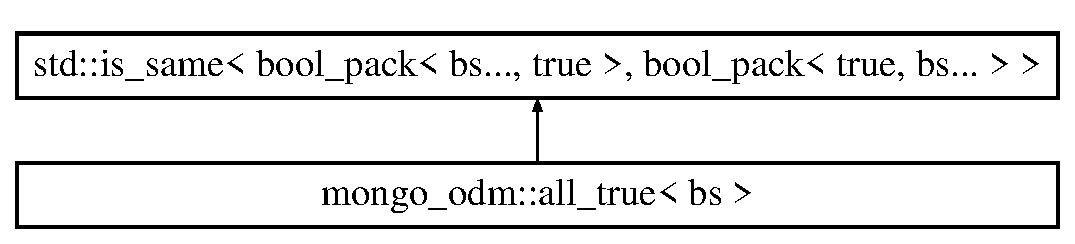
\includegraphics[height=2.000000cm]{structmongo__odm_1_1all__true}
\end{center}
\end{figure}


\subsection{Detailed Description}
\subsubsection*{template$<$bool... bs$>$\\*
struct mongo\+\_\+odm\+::all\+\_\+true$<$ bs $>$}

A templated struct for determining whether a variadic list of boolean conditions is all true. 

i.\+e. a logical A\+ND of a set of conditions. 

The documentation for this struct was generated from the following file\+:\begin{DoxyCompactItemize}
\item 
src/mongo\+\_\+odm/util.\+hpp\end{DoxyCompactItemize}

\hypertarget{classmongo__odm_1_1array__element__nvp}{}\section{mongo\+\_\+odm\+:\+:array\+\_\+element\+\_\+nvp$<$ NvpT $>$ Class Template Reference}
\label{classmongo__odm_1_1array__element__nvp}\index{mongo\+\_\+odm\+::array\+\_\+element\+\_\+nvp$<$ Nvp\+T $>$@{mongo\+\_\+odm\+::array\+\_\+element\+\_\+nvp$<$ Nvp\+T $>$}}
Inheritance diagram for mongo\+\_\+odm\+:\+:array\+\_\+element\+\_\+nvp$<$ NvpT $>$\+:\begin{figure}[H]
\begin{center}
\leavevmode
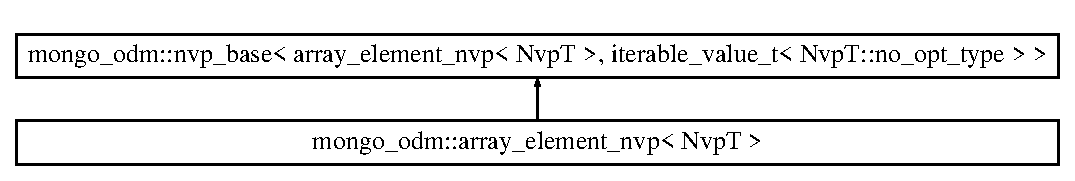
\includegraphics[height=1.989343cm]{classmongo__odm_1_1array__element__nvp}
\end{center}
\end{figure}
\subsection*{Public Member Functions}
\begin{DoxyCompactItemize}
\item 
constexpr \hyperlink{classmongo__odm_1_1update__expr}{update\+\_\+expr}$<$ \hyperlink{classmongo__odm_1_1array__element__nvp}{array\+\_\+element\+\_\+nvp}$<$ NvpT $>$, no\+\_\+opt\+\_\+type $>$ \hyperlink{classmongo__odm_1_1array__element__nvp_a92f296a58c7eeeda4aa847c7e98308a8}{operator=} (const no\+\_\+opt\+\_\+type \&val) const \hypertarget{classmongo__odm_1_1array__element__nvp_a92f296a58c7eeeda4aa847c7e98308a8}{}\label{classmongo__odm_1_1array__element__nvp_a92f296a58c7eeeda4aa847c7e98308a8}

\begin{DoxyCompactList}\small\item\em Creates an update expression that sets the field to the given value. \end{DoxyCompactList}\item 
std\+::string \hyperlink{classmongo__odm_1_1array__element__nvp_a910b3a4d344ad4bcecfb83bd4105f7e3}{get\+\_\+name} () const 
\begin{DoxyCompactList}\small\item\em Returns the qualified name of this field in dot notation, i.\+e. \end{DoxyCompactList}\item 
std\+::string \& \hyperlink{classmongo__odm_1_1array__element__nvp_ac3c14d806529b80826f97d4df17ff9b3}{append\+\_\+name} (std\+::string \&s) const 
\begin{DoxyCompactList}\small\item\em Returns the qualified name of this field in dot notation, i.\+e. \end{DoxyCompactList}\end{DoxyCompactItemize}


\subsection{Member Function Documentation}
\index{mongo\+\_\+odm\+::array\+\_\+element\+\_\+nvp@{mongo\+\_\+odm\+::array\+\_\+element\+\_\+nvp}!append\+\_\+name@{append\+\_\+name}}
\index{append\+\_\+name@{append\+\_\+name}!mongo\+\_\+odm\+::array\+\_\+element\+\_\+nvp@{mongo\+\_\+odm\+::array\+\_\+element\+\_\+nvp}}
\subsubsection[{\texorpdfstring{append\+\_\+name(std\+::string \&s) const }{append_name(std::string &s) const }}]{\setlength{\rightskip}{0pt plus 5cm}template$<$typename NvpT $>$ std\+::string\& {\bf mongo\+\_\+odm\+::array\+\_\+element\+\_\+nvp}$<$ NvpT $>$\+::append\+\_\+name (
\begin{DoxyParamCaption}
\item[{std\+::string \&}]{s}
\end{DoxyParamCaption}
) const\hspace{0.3cm}{\ttfamily [inline]}}\hypertarget{classmongo__odm_1_1array__element__nvp_ac3c14d806529b80826f97d4df17ff9b3}{}\label{classmongo__odm_1_1array__element__nvp_ac3c14d806529b80826f97d4df17ff9b3}


Returns the qualified name of this field in dot notation, i.\+e. 

\char`\"{}field.$<$index$>$\char`\"{}, where index is a number. \begin{DoxyReturn}{Returns}
A string containing the name of this field in dot notation. 
\end{DoxyReturn}
\index{mongo\+\_\+odm\+::array\+\_\+element\+\_\+nvp@{mongo\+\_\+odm\+::array\+\_\+element\+\_\+nvp}!get\+\_\+name@{get\+\_\+name}}
\index{get\+\_\+name@{get\+\_\+name}!mongo\+\_\+odm\+::array\+\_\+element\+\_\+nvp@{mongo\+\_\+odm\+::array\+\_\+element\+\_\+nvp}}
\subsubsection[{\texorpdfstring{get\+\_\+name() const }{get_name() const }}]{\setlength{\rightskip}{0pt plus 5cm}template$<$typename NvpT $>$ std\+::string {\bf mongo\+\_\+odm\+::array\+\_\+element\+\_\+nvp}$<$ NvpT $>$\+::get\+\_\+name (
\begin{DoxyParamCaption}
{}
\end{DoxyParamCaption}
) const\hspace{0.3cm}{\ttfamily [inline]}}\hypertarget{classmongo__odm_1_1array__element__nvp_a910b3a4d344ad4bcecfb83bd4105f7e3}{}\label{classmongo__odm_1_1array__element__nvp_a910b3a4d344ad4bcecfb83bd4105f7e3}


Returns the qualified name of this field in dot notation, i.\+e. 

\char`\"{}array.\+i\char`\"{}. \begin{DoxyReturn}{Returns}
A string containing the name of this field in dot notation. 
\end{DoxyReturn}


The documentation for this class was generated from the following file\+:\begin{DoxyCompactItemize}
\item 
src/mongo\+\_\+odm/nvp.\+hpp\end{DoxyCompactItemize}

\hypertarget{classmongo__odm_1_1bit__update__expr}{}\section{mongo\+\_\+odm\+:\+:bit\+\_\+update\+\_\+expr$<$ NvpT, Integer $>$ Class Template Reference}
\label{classmongo__odm_1_1bit__update__expr}\index{mongo\+\_\+odm\+::bit\+\_\+update\+\_\+expr$<$ Nvp\+T, Integer $>$@{mongo\+\_\+odm\+::bit\+\_\+update\+\_\+expr$<$ Nvp\+T, Integer $>$}}


Expression that updates field using the \$bit operator, which does bitwise operations using a mask.  




{\ttfamily \#include $<$query\+\_\+builder.\+hpp$>$}

\subsection*{Public Member Functions}
\begin{DoxyCompactItemize}
\item 
void \hyperlink{classmongo__odm_1_1bit__update__expr_a3376a71ac3c15a2ea7ac0e297e5bd59d}{append\+\_\+to\+\_\+bson} (bsoncxx\+::builder\+::core \&builder, bool wrap=false) const 
\begin{DoxyCompactList}\small\item\em Appends this query to a B\+S\+ON core builder as an expression \textquotesingle{}\$bit\+: \{ $<$field$>$\+: \{ $<$and$\vert$or$\vert$xor$>$\+: $<$int$>$ \} \}\textquotesingle{}. \end{DoxyCompactList}\end{DoxyCompactItemize}


\subsection{Detailed Description}
\subsubsection*{template$<$typename NvpT, typename Integer$>$\\*
class mongo\+\_\+odm\+::bit\+\_\+update\+\_\+expr$<$ Nvp\+T, Integer $>$}

Expression that updates field using the \$bit operator, which does bitwise operations using a mask. 


\begin{DoxyTemplParams}{Template Parameters}
{\em NvpT} & The name-\/value-\/pair type corresponding to a field \\
\hline
{\em Integer} & The integral type used as a bit mask \\
\hline
\end{DoxyTemplParams}


\subsection{Member Function Documentation}
\index{mongo\+\_\+odm\+::bit\+\_\+update\+\_\+expr@{mongo\+\_\+odm\+::bit\+\_\+update\+\_\+expr}!append\+\_\+to\+\_\+bson@{append\+\_\+to\+\_\+bson}}
\index{append\+\_\+to\+\_\+bson@{append\+\_\+to\+\_\+bson}!mongo\+\_\+odm\+::bit\+\_\+update\+\_\+expr@{mongo\+\_\+odm\+::bit\+\_\+update\+\_\+expr}}
\subsubsection[{\texorpdfstring{append\+\_\+to\+\_\+bson(bsoncxx\+::builder\+::core \&builder, bool wrap=false) const }{append_to_bson(bsoncxx::builder::core &builder, bool wrap=false) const }}]{\setlength{\rightskip}{0pt plus 5cm}template$<$typename NvpT , typename Integer $>$ void {\bf mongo\+\_\+odm\+::bit\+\_\+update\+\_\+expr}$<$ NvpT, Integer $>$\+::append\+\_\+to\+\_\+bson (
\begin{DoxyParamCaption}
\item[{bsoncxx\+::builder\+::core \&}]{builder, }
\item[{bool}]{wrap = {\ttfamily false}}
\end{DoxyParamCaption}
) const\hspace{0.3cm}{\ttfamily [inline]}}\hypertarget{classmongo__odm_1_1bit__update__expr_a3376a71ac3c15a2ea7ac0e297e5bd59d}{}\label{classmongo__odm_1_1bit__update__expr_a3376a71ac3c15a2ea7ac0e297e5bd59d}


Appends this query to a B\+S\+ON core builder as an expression \textquotesingle{}\$bit\+: \{ $<$field$>$\+: \{ $<$and$\vert$or$\vert$xor$>$\+: $<$int$>$ \} \}\textquotesingle{}. 


\begin{DoxyParams}{Parameters}
{\em builder} & A basic B\+S\+ON core builder. \\
\hline
{\em Whether} & to wrap this expression inside a document. \\
\hline
\end{DoxyParams}


The documentation for this class was generated from the following files\+:\begin{DoxyCompactItemize}
\item 
src/mongo\+\_\+odm/expression\+\_\+syntax.\+hpp\item 
src/mongo\+\_\+odm/query\+\_\+builder.\+hpp\end{DoxyCompactItemize}

\hypertarget{structmongo__odm_1_1bool__pack}{}\section{mongo\+\_\+odm\+:\+:bool\+\_\+pack$<$... $>$ Struct Template Reference}
\label{structmongo__odm_1_1bool__pack}\index{mongo\+\_\+odm\+::bool\+\_\+pack$<$... $>$@{mongo\+\_\+odm\+::bool\+\_\+pack$<$... $>$}}


The documentation for this struct was generated from the following file\+:\begin{DoxyCompactItemize}
\item 
src/mongo\+\_\+odm/util.\+hpp\end{DoxyCompactItemize}

\hypertarget{classmongo__odm_1_1boolean__expr}{}\section{mongo\+\_\+odm\+:\+:boolean\+\_\+expr$<$ Expr1, Expr2 $>$ Class Template Reference}
\label{classmongo__odm_1_1boolean__expr}\index{mongo\+\_\+odm\+::boolean\+\_\+expr$<$ Expr1, Expr2 $>$@{mongo\+\_\+odm\+::boolean\+\_\+expr$<$ Expr1, Expr2 $>$}}


This represents a boolean expression with two arguments.  




{\ttfamily \#include $<$query\+\_\+builder.\+hpp$>$}

\subsection*{Public Member Functions}
\begin{DoxyCompactItemize}
\item 
constexpr \hyperlink{classmongo__odm_1_1boolean__expr_a78c7a59f9f857fe8d5609493f155d96a}{boolean\+\_\+expr} (const Expr1 \&lhs, const Expr2 \&rhs, const char $\ast$op)
\begin{DoxyCompactList}\small\item\em Constructs a boolean expression from two other expressions, and a certain operator. \end{DoxyCompactList}\item 
void \hyperlink{classmongo__odm_1_1boolean__expr_ad74cd57820615fe960f4489af2091bbd}{append\+\_\+to\+\_\+bson} (bsoncxx\+::builder\+::core \&builder, bool wrap=false) const 
\begin{DoxyCompactList}\small\item\em Appends this query to a B\+S\+ON core builder as a key-\/value pair \char`\"{}\$op\+: \mbox{[}\{lhs\}, \{rhs\}\mbox{]}\char`\"{}. \end{DoxyCompactList}\item 
\hyperlink{classmongo__odm_1_1boolean__expr_af5fb062846c5f8fb95a8333ad9723006}{operator bsoncxx\+::document\+::view\+\_\+or\+\_\+value} () const \hypertarget{classmongo__odm_1_1boolean__expr_af5fb062846c5f8fb95a8333ad9723006}{}\label{classmongo__odm_1_1boolean__expr_af5fb062846c5f8fb95a8333ad9723006}

\begin{DoxyCompactList}\small\item\em Converts the expression to a B\+S\+ON filter for a query, in the form \char`\"{}\{ \$op\+: \mbox{[}\{lhs\}, \{rhs\}\mbox{]} \}\char`\"{}. \end{DoxyCompactList}\end{DoxyCompactItemize}


\subsection{Detailed Description}
\subsubsection*{template$<$typename Expr1, typename Expr2$>$\\*
class mongo\+\_\+odm\+::boolean\+\_\+expr$<$ Expr1, Expr2 $>$}

This represents a boolean expression with two arguments. 

The arguments can, in turn, be boolean expressions. 

\subsection{Constructor \& Destructor Documentation}
\index{mongo\+\_\+odm\+::boolean\+\_\+expr@{mongo\+\_\+odm\+::boolean\+\_\+expr}!boolean\+\_\+expr@{boolean\+\_\+expr}}
\index{boolean\+\_\+expr@{boolean\+\_\+expr}!mongo\+\_\+odm\+::boolean\+\_\+expr@{mongo\+\_\+odm\+::boolean\+\_\+expr}}
\subsubsection[{\texorpdfstring{boolean\+\_\+expr(const Expr1 \&lhs, const Expr2 \&rhs, const char $\ast$op)}{boolean_expr(const Expr1 &lhs, const Expr2 &rhs, const char *op)}}]{\setlength{\rightskip}{0pt plus 5cm}template$<$typename Expr1 , typename Expr2 $>$ constexpr {\bf mongo\+\_\+odm\+::boolean\+\_\+expr}$<$ Expr1, Expr2 $>$\+::{\bf boolean\+\_\+expr} (
\begin{DoxyParamCaption}
\item[{const Expr1 \&}]{lhs, }
\item[{const Expr2 \&}]{rhs, }
\item[{const char $\ast$}]{op}
\end{DoxyParamCaption}
)\hspace{0.3cm}{\ttfamily [inline]}}\hypertarget{classmongo__odm_1_1boolean__expr_a78c7a59f9f857fe8d5609493f155d96a}{}\label{classmongo__odm_1_1boolean__expr_a78c7a59f9f857fe8d5609493f155d96a}


Constructs a boolean expression from two other expressions, and a certain operator. 


\begin{DoxyParams}{Parameters}
{\em lhs} & The left-\/hand side of the expression. \\
\hline
{\em rhs} & The right-\/hand side of the expression. \\
\hline
{\em op} & The operator of the expression, e.\+g. A\+ND or OR. \\
\hline
\end{DoxyParams}


\subsection{Member Function Documentation}
\index{mongo\+\_\+odm\+::boolean\+\_\+expr@{mongo\+\_\+odm\+::boolean\+\_\+expr}!append\+\_\+to\+\_\+bson@{append\+\_\+to\+\_\+bson}}
\index{append\+\_\+to\+\_\+bson@{append\+\_\+to\+\_\+bson}!mongo\+\_\+odm\+::boolean\+\_\+expr@{mongo\+\_\+odm\+::boolean\+\_\+expr}}
\subsubsection[{\texorpdfstring{append\+\_\+to\+\_\+bson(bsoncxx\+::builder\+::core \&builder, bool wrap=false) const }{append_to_bson(bsoncxx::builder::core &builder, bool wrap=false) const }}]{\setlength{\rightskip}{0pt plus 5cm}template$<$typename Expr1 , typename Expr2 $>$ void {\bf mongo\+\_\+odm\+::boolean\+\_\+expr}$<$ Expr1, Expr2 $>$\+::append\+\_\+to\+\_\+bson (
\begin{DoxyParamCaption}
\item[{bsoncxx\+::builder\+::core \&}]{builder, }
\item[{bool}]{wrap = {\ttfamily false}}
\end{DoxyParamCaption}
) const\hspace{0.3cm}{\ttfamily [inline]}}\hypertarget{classmongo__odm_1_1boolean__expr_ad74cd57820615fe960f4489af2091bbd}{}\label{classmongo__odm_1_1boolean__expr_ad74cd57820615fe960f4489af2091bbd}


Appends this query to a B\+S\+ON core builder as a key-\/value pair \char`\"{}\$op\+: \mbox{[}\{lhs\}, \{rhs\}\mbox{]}\char`\"{}. 


\begin{DoxyParams}{Parameters}
{\em builder} & A basic B\+S\+ON core builder. \\
\hline
{\em Whether} & to wrap this expression inside a document. \\
\hline
\end{DoxyParams}


The documentation for this class was generated from the following files\+:\begin{DoxyCompactItemize}
\item 
src/mongo\+\_\+odm/expression\+\_\+syntax.\+hpp\item 
src/mongo\+\_\+odm/query\+\_\+builder.\+hpp\end{DoxyCompactItemize}

\hypertarget{classmongo__odm_1_1boolean__list__expr}{}\section{mongo\+\_\+odm\+:\+:boolean\+\_\+list\+\_\+expr$<$ List $>$ Class Template Reference}
\label{classmongo__odm_1_1boolean__list__expr}\index{mongo\+\_\+odm\+::boolean\+\_\+list\+\_\+expr$<$ List $>$@{mongo\+\_\+odm\+::boolean\+\_\+list\+\_\+expr$<$ List $>$}}


This class represents a boolean expression over an array of arguments.  




{\ttfamily \#include $<$query\+\_\+builder.\+hpp$>$}

\subsection*{Public Member Functions}
\begin{DoxyCompactItemize}
\item 
constexpr \hyperlink{classmongo__odm_1_1boolean__list__expr_a71f9da341b80a5bd5062c8ec627a9241}{boolean\+\_\+list\+\_\+expr} (const List args, const char $\ast$op)
\begin{DoxyCompactList}\small\item\em Constructs a boolean expression from a list of sub-\/expressions, and a certain operator. \end{DoxyCompactList}\item 
void \hyperlink{classmongo__odm_1_1boolean__list__expr_a5aa985b42f30ceb49fa6a5481693aa8a}{append\+\_\+to\+\_\+bson} (bsoncxx\+::builder\+::core \&builder, bool wrap=false) const 
\begin{DoxyCompactList}\small\item\em Appends this query to a B\+S\+ON core builder as a key-\/value pair \char`\"{}\$op\+: \mbox{[}\{lhs\}, \{rhs\}\mbox{]}\char`\"{}. \end{DoxyCompactList}\item 
\hyperlink{classmongo__odm_1_1boolean__list__expr_aec500b9de32ab2dbe8550aeccc1115ca}{operator bsoncxx\+::document\+::view\+\_\+or\+\_\+value} () const \hypertarget{classmongo__odm_1_1boolean__list__expr_aec500b9de32ab2dbe8550aeccc1115ca}{}\label{classmongo__odm_1_1boolean__list__expr_aec500b9de32ab2dbe8550aeccc1115ca}

\begin{DoxyCompactList}\small\item\em Converts the expression to a B\+S\+ON filter for a query, in the form \char`\"{}\{\$op\+: \mbox{[}\{arg1\}, \{arg2\}, ...\mbox{]}\}\char`\"{}. \end{DoxyCompactList}\end{DoxyCompactItemize}


\subsection{Detailed Description}
\subsubsection*{template$<$typename List$>$\\*
class mongo\+\_\+odm\+::boolean\+\_\+list\+\_\+expr$<$ List $>$}

This class represents a boolean expression over an array of arguments. 

This is particularly useful for the \$nor operator. When converted to B\+S\+ON, this class produces an expression \{\$op\+: \mbox{[}\{arg1\}, \{arg2\}, ...\mbox{]}\} 

\subsection{Constructor \& Destructor Documentation}
\index{mongo\+\_\+odm\+::boolean\+\_\+list\+\_\+expr@{mongo\+\_\+odm\+::boolean\+\_\+list\+\_\+expr}!boolean\+\_\+list\+\_\+expr@{boolean\+\_\+list\+\_\+expr}}
\index{boolean\+\_\+list\+\_\+expr@{boolean\+\_\+list\+\_\+expr}!mongo\+\_\+odm\+::boolean\+\_\+list\+\_\+expr@{mongo\+\_\+odm\+::boolean\+\_\+list\+\_\+expr}}
\subsubsection[{\texorpdfstring{boolean\+\_\+list\+\_\+expr(const List args, const char $\ast$op)}{boolean_list_expr(const List args, const char *op)}}]{\setlength{\rightskip}{0pt plus 5cm}template$<$typename List $>$ constexpr {\bf mongo\+\_\+odm\+::boolean\+\_\+list\+\_\+expr}$<$ List $>$\+::{\bf boolean\+\_\+list\+\_\+expr} (
\begin{DoxyParamCaption}
\item[{const List}]{args, }
\item[{const char $\ast$}]{op}
\end{DoxyParamCaption}
)\hspace{0.3cm}{\ttfamily [inline]}}\hypertarget{classmongo__odm_1_1boolean__list__expr_a71f9da341b80a5bd5062c8ec627a9241}{}\label{classmongo__odm_1_1boolean__list__expr_a71f9da341b80a5bd5062c8ec627a9241}


Constructs a boolean expression from a list of sub-\/expressions, and a certain operator. 


\begin{DoxyParams}{Parameters}
{\em args} & An expression list of boolean conditions. \\
\hline
{\em op} & The operator of the expression, e.\+g. A\+ND or OR. \\
\hline
\end{DoxyParams}


\subsection{Member Function Documentation}
\index{mongo\+\_\+odm\+::boolean\+\_\+list\+\_\+expr@{mongo\+\_\+odm\+::boolean\+\_\+list\+\_\+expr}!append\+\_\+to\+\_\+bson@{append\+\_\+to\+\_\+bson}}
\index{append\+\_\+to\+\_\+bson@{append\+\_\+to\+\_\+bson}!mongo\+\_\+odm\+::boolean\+\_\+list\+\_\+expr@{mongo\+\_\+odm\+::boolean\+\_\+list\+\_\+expr}}
\subsubsection[{\texorpdfstring{append\+\_\+to\+\_\+bson(bsoncxx\+::builder\+::core \&builder, bool wrap=false) const }{append_to_bson(bsoncxx::builder::core &builder, bool wrap=false) const }}]{\setlength{\rightskip}{0pt plus 5cm}template$<$typename List $>$ void {\bf mongo\+\_\+odm\+::boolean\+\_\+list\+\_\+expr}$<$ List $>$\+::append\+\_\+to\+\_\+bson (
\begin{DoxyParamCaption}
\item[{bsoncxx\+::builder\+::core \&}]{builder, }
\item[{bool}]{wrap = {\ttfamily false}}
\end{DoxyParamCaption}
) const\hspace{0.3cm}{\ttfamily [inline]}}\hypertarget{classmongo__odm_1_1boolean__list__expr_a5aa985b42f30ceb49fa6a5481693aa8a}{}\label{classmongo__odm_1_1boolean__list__expr_a5aa985b42f30ceb49fa6a5481693aa8a}


Appends this query to a B\+S\+ON core builder as a key-\/value pair \char`\"{}\$op\+: \mbox{[}\{lhs\}, \{rhs\}\mbox{]}\char`\"{}. 


\begin{DoxyParams}{Parameters}
{\em builder} & A basic B\+S\+ON core builder. \\
\hline
{\em wrap} & Whether to wrap this expression inside a document. \\
\hline
\end{DoxyParams}


The documentation for this class was generated from the following files\+:\begin{DoxyCompactItemize}
\item 
src/mongo\+\_\+odm/expression\+\_\+syntax.\+hpp\item 
src/mongo\+\_\+odm/query\+\_\+builder.\+hpp\end{DoxyCompactItemize}

\hypertarget{classbson__mapper_1_1bson__input__streambuf}{}\section{bson\+\_\+mapper\+:\+:bson\+\_\+input\+\_\+streambuf Class Reference}
\label{classbson__mapper_1_1bson__input__streambuf}\index{bson\+\_\+mapper\+::bson\+\_\+input\+\_\+streambuf@{bson\+\_\+mapper\+::bson\+\_\+input\+\_\+streambuf}}


A wrapper from \hyperlink{classbson__mapper_1_1char__array__streambuf}{char\+\_\+array\+\_\+streambuf}, that uses the data from a B\+S\+ON document view as a buffer.  




{\ttfamily \#include $<$bson\+\_\+streambuf.\+hpp$>$}

Inheritance diagram for bson\+\_\+mapper\+:\+:bson\+\_\+input\+\_\+streambuf\+:\begin{figure}[H]
\begin{center}
\leavevmode
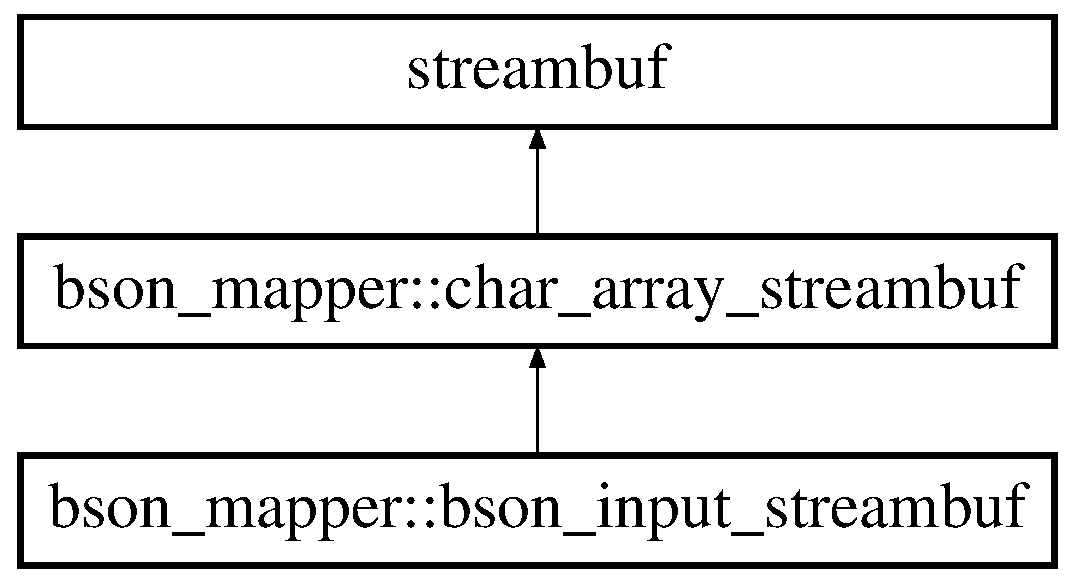
\includegraphics[height=3.000000cm]{classbson__mapper_1_1bson__input__streambuf}
\end{center}
\end{figure}
\subsection*{Additional Inherited Members}


\subsection{Detailed Description}
A wrapper from \hyperlink{classbson__mapper_1_1char__array__streambuf}{char\+\_\+array\+\_\+streambuf}, that uses the data from a B\+S\+ON document view as a buffer. 

The documentation for this class was generated from the following file\+:\begin{DoxyCompactItemize}
\item 
src/bson\+\_\+mapper/bson\+\_\+streambuf.\+hpp\end{DoxyCompactItemize}

\hypertarget{classbson__mapper_1_1bson__istream}{}\section{bson\+\_\+mapper\+:\+:bson\+\_\+istream Class Reference}
\label{classbson__mapper_1_1bson__istream}\index{bson\+\_\+mapper\+::bson\+\_\+istream@{bson\+\_\+mapper\+::bson\+\_\+istream}}


An istream that uses a B\+S\+ON document as a buffer.  




{\ttfamily \#include $<$bson\+\_\+streambuf.\+hpp$>$}

Inheritance diagram for bson\+\_\+mapper\+:\+:bson\+\_\+istream\+:\begin{figure}[H]
\begin{center}
\leavevmode
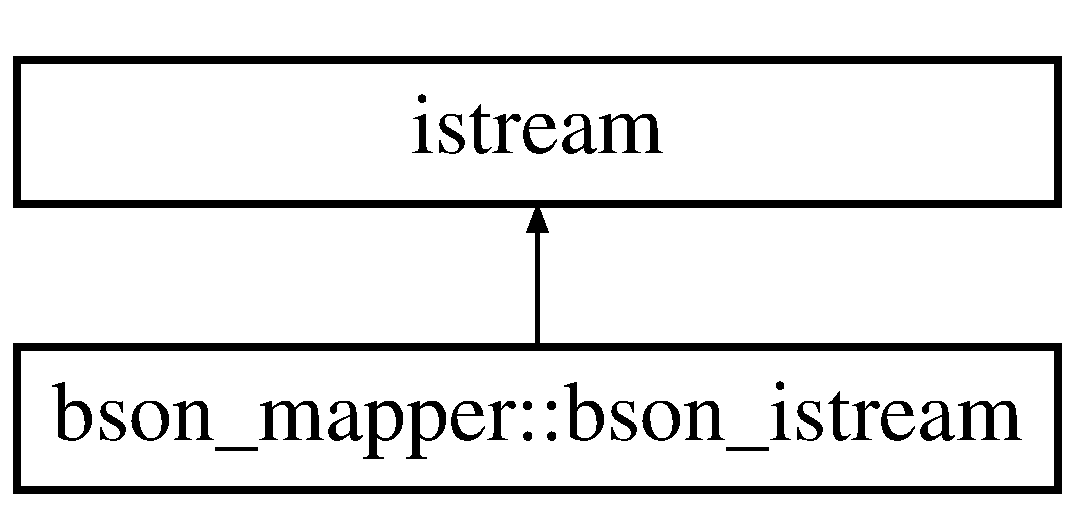
\includegraphics[height=2.000000cm]{classbson__mapper_1_1bson__istream}
\end{center}
\end{figure}


\subsection{Detailed Description}
An istream that uses a B\+S\+ON document as a buffer. 

While objects of this class do not own the underlying buffer, they do own the streambuf object associated with it.

By default, istream objects do not delete their streambuffers when they are destroyed, so this class allows one to create a stream without dealing with the underlying streambuf object. 

The documentation for this class was generated from the following file\+:\begin{DoxyCompactItemize}
\item 
src/bson\+\_\+mapper/bson\+\_\+streambuf.\+hpp\end{DoxyCompactItemize}

\hypertarget{classbson__mapper_1_1bson__ostream}{}\section{bson\+\_\+mapper\+:\+:bson\+\_\+ostream Class Reference}
\label{classbson__mapper_1_1bson__ostream}\index{bson\+\_\+mapper\+::bson\+\_\+ostream@{bson\+\_\+mapper\+::bson\+\_\+ostream}}


An ostream that writes bytes of B\+S\+ON documents into a collection.  




{\ttfamily \#include $<$bson\+\_\+streambuf.\+hpp$>$}

Inheritance diagram for bson\+\_\+mapper\+:\+:bson\+\_\+ostream\+:\begin{figure}[H]
\begin{center}
\leavevmode
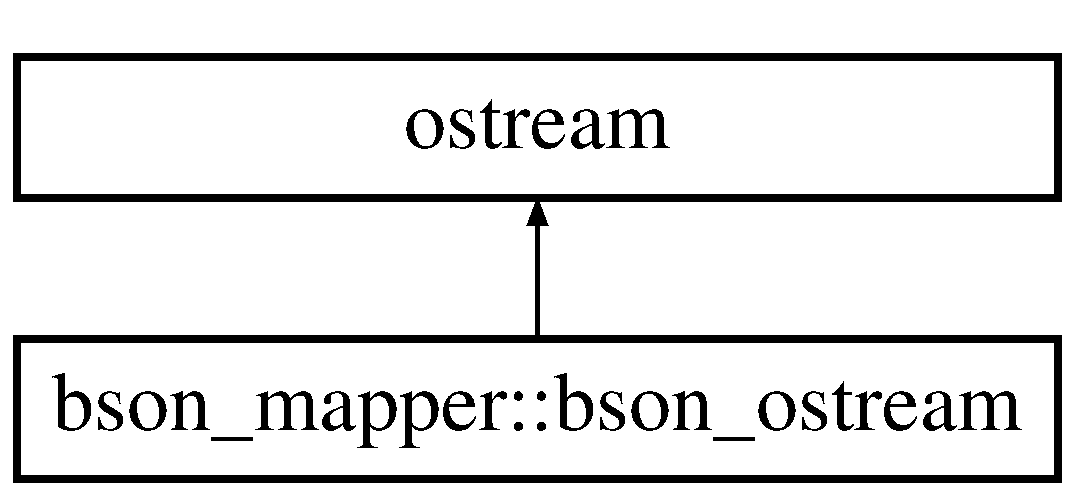
\includegraphics[height=2.000000cm]{classbson__mapper_1_1bson__ostream}
\end{center}
\end{figure}


\subsection{Detailed Description}
An ostream that writes bytes of B\+S\+ON documents into a collection. 

The stream owns its own \hyperlink{classbson__mapper_1_1bson__output__streambuf}{bson\+\_\+output\+\_\+streambuf} object, making creation and management of such streams easier. 

The documentation for this class was generated from the following file\+:\begin{DoxyCompactItemize}
\item 
src/bson\+\_\+mapper/bson\+\_\+streambuf.\+hpp\end{DoxyCompactItemize}

\hypertarget{classbson__mapper_1_1bson__output__streambuf}{}\section{bson\+\_\+mapper\+:\+:bson\+\_\+output\+\_\+streambuf Class Reference}
\label{classbson__mapper_1_1bson__output__streambuf}\index{bson\+\_\+mapper\+::bson\+\_\+output\+\_\+streambuf@{bson\+\_\+mapper\+::bson\+\_\+output\+\_\+streambuf}}


A streambuffer that accepts one or more B\+S\+ON documents as bytes of B\+S\+ON data.  




{\ttfamily \#include $<$bson\+\_\+streambuf.\+hpp$>$}

Inheritance diagram for bson\+\_\+mapper\+:\+:bson\+\_\+output\+\_\+streambuf\+:\begin{figure}[H]
\begin{center}
\leavevmode
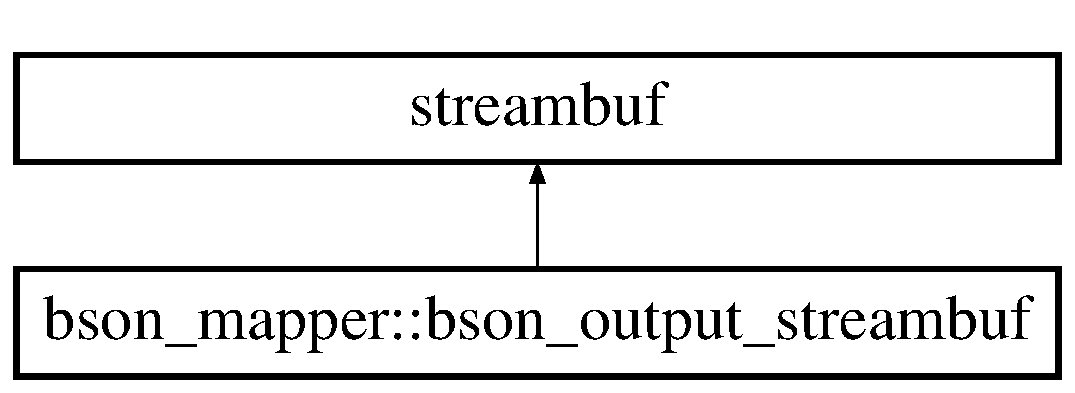
\includegraphics[height=2.000000cm]{classbson__mapper_1_1bson__output__streambuf}
\end{center}
\end{figure}
\subsection*{Public Member Functions}
\begin{DoxyCompactItemize}
\item 
\hyperlink{classbson__mapper_1_1bson__output__streambuf_afbbff25db476b5ec8c166a030664579a}{bson\+\_\+output\+\_\+streambuf} (document\+\_\+callback cb)
\begin{DoxyCompactList}\small\item\em Constructs a new B\+S\+ON Output Streambuffer that passes documents to the given callback function. \end{DoxyCompactList}\item 
int \hyperlink{classbson__mapper_1_1bson__output__streambuf_aebf518d6dd7cad563dced7299b05456e}{overflow} (int ch) override
\begin{DoxyCompactList}\small\item\em This function is called when writing to the stream and the buffer is full. \end{DoxyCompactList}\item 
virtual int \hyperlink{classbson__mapper_1_1bson__output__streambuf_abf1753938d33b31f2408967589ca64ee}{underflow} () override
\begin{DoxyCompactList}\small\item\em This function always returns E\+OF, since one should not write from an output stream. \end{DoxyCompactList}\end{DoxyCompactItemize}


\subsection{Detailed Description}
A streambuffer that accepts one or more B\+S\+ON documents as bytes of B\+S\+ON data. 

When a document is complete, it is passed into the user-\/provided callback. N\+O\+TE\+: This does not perform any validation on the B\+S\+ON files, and simply uses their first four bytes to judge the document length. 

\subsection{Constructor \& Destructor Documentation}
\index{bson\+\_\+mapper\+::bson\+\_\+output\+\_\+streambuf@{bson\+\_\+mapper\+::bson\+\_\+output\+\_\+streambuf}!bson\+\_\+output\+\_\+streambuf@{bson\+\_\+output\+\_\+streambuf}}
\index{bson\+\_\+output\+\_\+streambuf@{bson\+\_\+output\+\_\+streambuf}!bson\+\_\+mapper\+::bson\+\_\+output\+\_\+streambuf@{bson\+\_\+mapper\+::bson\+\_\+output\+\_\+streambuf}}
\subsubsection[{\texorpdfstring{bson\+\_\+output\+\_\+streambuf(document\+\_\+callback cb)}{bson_output_streambuf(document_callback cb)}}]{\setlength{\rightskip}{0pt plus 5cm}bson\+\_\+mapper\+::bson\+\_\+output\+\_\+streambuf\+::bson\+\_\+output\+\_\+streambuf (
\begin{DoxyParamCaption}
\item[{document\+\_\+callback}]{cb}
\end{DoxyParamCaption}
)}\hypertarget{classbson__mapper_1_1bson__output__streambuf_afbbff25db476b5ec8c166a030664579a}{}\label{classbson__mapper_1_1bson__output__streambuf_afbbff25db476b5ec8c166a030664579a}


Constructs a new B\+S\+ON Output Streambuffer that passes documents to the given callback function. 


\begin{DoxyParams}{Parameters}
{\em cb} & A function that takes a document\+::value and returns void. \\
\hline
\end{DoxyParams}


\subsection{Member Function Documentation}
\index{bson\+\_\+mapper\+::bson\+\_\+output\+\_\+streambuf@{bson\+\_\+mapper\+::bson\+\_\+output\+\_\+streambuf}!overflow@{overflow}}
\index{overflow@{overflow}!bson\+\_\+mapper\+::bson\+\_\+output\+\_\+streambuf@{bson\+\_\+mapper\+::bson\+\_\+output\+\_\+streambuf}}
\subsubsection[{\texorpdfstring{overflow(int ch) override}{overflow(int ch) override}}]{\setlength{\rightskip}{0pt plus 5cm}int bson\+\_\+mapper\+::bson\+\_\+output\+\_\+streambuf\+::overflow (
\begin{DoxyParamCaption}
\item[{int}]{ch}
\end{DoxyParamCaption}
)\hspace{0.3cm}{\ttfamily [override]}}\hypertarget{classbson__mapper_1_1bson__output__streambuf_aebf518d6dd7cad563dced7299b05456e}{}\label{classbson__mapper_1_1bson__output__streambuf_aebf518d6dd7cad563dced7299b05456e}


This function is called when writing to the stream and the buffer is full. 

Since we don\textquotesingle{}t define a buffer, this is called with every character. 
\begin{DoxyParams}{Parameters}
{\em ch} & The byte of B\+S\+ON to insert. \\
\hline
\end{DoxyParams}
\begin{DoxyReturn}{Returns}
The inserted byte, or E\+OF if something failed. 
\end{DoxyReturn}
\index{bson\+\_\+mapper\+::bson\+\_\+output\+\_\+streambuf@{bson\+\_\+mapper\+::bson\+\_\+output\+\_\+streambuf}!underflow@{underflow}}
\index{underflow@{underflow}!bson\+\_\+mapper\+::bson\+\_\+output\+\_\+streambuf@{bson\+\_\+mapper\+::bson\+\_\+output\+\_\+streambuf}}
\subsubsection[{\texorpdfstring{underflow() override}{underflow() override}}]{\setlength{\rightskip}{0pt plus 5cm}virtual int bson\+\_\+mapper\+::bson\+\_\+output\+\_\+streambuf\+::underflow (
\begin{DoxyParamCaption}
{}
\end{DoxyParamCaption}
)\hspace{0.3cm}{\ttfamily [override]}, {\ttfamily [virtual]}}\hypertarget{classbson__mapper_1_1bson__output__streambuf_abf1753938d33b31f2408967589ca64ee}{}\label{classbson__mapper_1_1bson__output__streambuf_abf1753938d33b31f2408967589ca64ee}


This function always returns E\+OF, since one should not write from an output stream. 

\begin{DoxyReturn}{Returns}
E\+OF 
\end{DoxyReturn}


The documentation for this class was generated from the following file\+:\begin{DoxyCompactItemize}
\item 
src/bson\+\_\+mapper/bson\+\_\+streambuf.\+hpp\end{DoxyCompactItemize}

\hypertarget{classbson__mapper_1_1BSONInputArchive}{}\section{bson\+\_\+mapper\+:\+:B\+S\+O\+N\+Input\+Archive Class Reference}
\label{classbson__mapper_1_1BSONInputArchive}\index{bson\+\_\+mapper\+::\+B\+S\+O\+N\+Input\+Archive@{bson\+\_\+mapper\+::\+B\+S\+O\+N\+Input\+Archive}}
Inheritance diagram for bson\+\_\+mapper\+:\+:B\+S\+O\+N\+Input\+Archive\+:\begin{figure}[H]
\begin{center}
\leavevmode
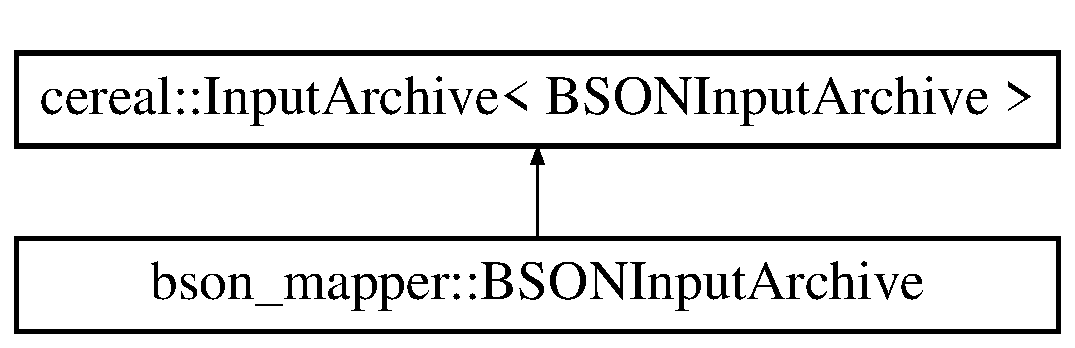
\includegraphics[height=2.000000cm]{classbson__mapper_1_1BSONInputArchive}
\end{center}
\end{figure}
\subsection*{Public Member Functions}
\begin{DoxyCompactItemize}
\item 
\hyperlink{classbson__mapper_1_1BSONInputArchive_a6b8ddbbd18800ef0f8e250c31da095e8}{B\+S\+O\+N\+Input\+Archive} (std\+::istream \&stream)
\begin{DoxyCompactList}\small\item\em Construct a \hyperlink{classbson__mapper_1_1BSONInputArchive}{B\+S\+O\+N\+Input\+Archive} from an input stream of B\+S\+ON data. \end{DoxyCompactList}\item 
bool \hyperlink{classbson__mapper_1_1BSONInputArchive_a0b8d043db14caa7d4e35d8e5300cd69f}{will\+Search\+Yield\+Value} ()
\begin{DoxyCompactList}\small\item\em Checks if the next invocation of search() will yield a value. \end{DoxyCompactList}\item 
bool \hyperlink{classbson__mapper_1_1BSONInputArchive_ab0b224d34f6dd2fd9ee542571536638b}{start\+Root\+Element\+If\+Root} ()
\begin{DoxyCompactList}\small\item\em Pushes a root element on the node stack if we\textquotesingle{}re in root. \end{DoxyCompactList}\item 
void \hyperlink{classbson__mapper_1_1BSONInputArchive_a1100f99901973ebefab2198d2381e953}{finish\+Root\+Element\+If\+Root\+Element} ()\hypertarget{classbson__mapper_1_1BSONInputArchive_a1100f99901973ebefab2198d2381e953}{}\label{classbson__mapper_1_1BSONInputArchive_a1100f99901973ebefab2198d2381e953}

\begin{DoxyCompactList}\small\item\em Pops the node stack and iterates to the next B\+S\+ON view if the top of the stack specifies that we are in a root element. \end{DoxyCompactList}\item 
void \hyperlink{classbson__mapper_1_1BSONInputArchive_a6f74b53f0989e9222be00dec0e6d350f}{start\+Node} ()\hypertarget{classbson__mapper_1_1BSONInputArchive_a6f74b53f0989e9222be00dec0e6d350f}{}\label{classbson__mapper_1_1BSONInputArchive_a6f74b53f0989e9222be00dec0e6d350f}

\begin{DoxyCompactList}\small\item\em Starts a new node, and update the stacks so that we fetch the correct data when calling search(). \end{DoxyCompactList}\item 
void \hyperlink{classbson__mapper_1_1BSONInputArchive_a9360961eba7c7c430329eed30667a2de}{finish\+Node} ()\hypertarget{classbson__mapper_1_1BSONInputArchive_a9360961eba7c7c430329eed30667a2de}{}\label{classbson__mapper_1_1BSONInputArchive_a9360961eba7c7c430329eed30667a2de}

\begin{DoxyCompactList}\small\item\em Finishes the most recently started node by popping relevant stacks and, if necessary, iterating to the next root B\+S\+ON document. \end{DoxyCompactList}\item 
void \hyperlink{classbson__mapper_1_1BSONInputArchive_a5536f703a1f8d0f19fca666290ee6b42}{set\+Next\+Name} (const char $\ast$name)
\begin{DoxyCompactList}\small\item\em Sets the name for the next node created with start\+Node. \end{DoxyCompactList}\item 
void \hyperlink{classbson__mapper_1_1BSONInputArchive_a457680690d03b26a9600b9139d1b9bd9}{load\+Value} (std\+::chrono\+::system\+\_\+clock\+::time\+\_\+point \&val)
\begin{DoxyCompactList}\small\item\em Loads a B\+S\+ON datetime from the current node and puts it into a std\+::chrono\+::system\+\_\+clock\+::time\+\_\+point. \end{DoxyCompactList}\item 
void \hyperlink{classbson__mapper_1_1BSONInputArchive_afa63fee8fca6808c51178fb6a7767abd}{load\+Value} (std\+::string \&val)
\begin{DoxyCompactList}\small\item\em Loads a B\+S\+ON U\+T\+F-\/8 value from the current node and puts it into a std\+::string. \end{DoxyCompactList}\item 
void \hyperlink{classbson__mapper_1_1BSONInputArchive_a28c16081fe45749c56f5d65b1ab01d40}{load\+Size} (cereal\+::size\+\_\+type \&size)
\begin{DoxyCompactList}\small\item\em Loads the size for a Size\+Tag, which is used by Cereal to determine how many elements to put into a container such as a std\+::vector. \end{DoxyCompactList}\item 
void \hyperlink{classbson__mapper_1_1BSONInputArchive_ad3fae22817ce463e8a3055a1f04e7a91}{load\+Underlying\+Data\+For\+Current\+Node} (\hyperlink{classbson__mapper_1_1UnderlyingBSONDataBase}{Underlying\+B\+S\+O\+N\+Data\+Base} \&underlying\+Data)\hypertarget{classbson__mapper_1_1BSONInputArchive_ad3fae22817ce463e8a3055a1f04e7a91}{}\label{classbson__mapper_1_1BSONInputArchive_ad3fae22817ce463e8a3055a1f04e7a91}

\begin{DoxyCompactList}\small\item\em Returns a shared pointer to the underlying data of the current node, loading the size in bytes in a size\+\_\+t reference argument. \end{DoxyCompactList}\end{DoxyCompactItemize}


\subsection{Constructor \& Destructor Documentation}
\index{bson\+\_\+mapper\+::\+B\+S\+O\+N\+Input\+Archive@{bson\+\_\+mapper\+::\+B\+S\+O\+N\+Input\+Archive}!B\+S\+O\+N\+Input\+Archive@{B\+S\+O\+N\+Input\+Archive}}
\index{B\+S\+O\+N\+Input\+Archive@{B\+S\+O\+N\+Input\+Archive}!bson\+\_\+mapper\+::\+B\+S\+O\+N\+Input\+Archive@{bson\+\_\+mapper\+::\+B\+S\+O\+N\+Input\+Archive}}
\subsubsection[{\texorpdfstring{B\+S\+O\+N\+Input\+Archive(std\+::istream \&stream)}{BSONInputArchive(std::istream &stream)}}]{\setlength{\rightskip}{0pt plus 5cm}bson\+\_\+mapper\+::\+B\+S\+O\+N\+Input\+Archive\+::\+B\+S\+O\+N\+Input\+Archive (
\begin{DoxyParamCaption}
\item[{std\+::istream \&}]{stream}
\end{DoxyParamCaption}
)\hspace{0.3cm}{\ttfamily [inline]}}\hypertarget{classbson__mapper_1_1BSONInputArchive_a6b8ddbbd18800ef0f8e250c31da095e8}{}\label{classbson__mapper_1_1BSONInputArchive_a6b8ddbbd18800ef0f8e250c31da095e8}


Construct a \hyperlink{classbson__mapper_1_1BSONInputArchive}{B\+S\+O\+N\+Input\+Archive} from an input stream of B\+S\+ON data. 


\begin{DoxyParams}{Parameters}
{\em stream} & The stream from which to read B\+S\+ON data. \\
\hline
\end{DoxyParams}


\subsection{Member Function Documentation}
\index{bson\+\_\+mapper\+::\+B\+S\+O\+N\+Input\+Archive@{bson\+\_\+mapper\+::\+B\+S\+O\+N\+Input\+Archive}!load\+Size@{load\+Size}}
\index{load\+Size@{load\+Size}!bson\+\_\+mapper\+::\+B\+S\+O\+N\+Input\+Archive@{bson\+\_\+mapper\+::\+B\+S\+O\+N\+Input\+Archive}}
\subsubsection[{\texorpdfstring{load\+Size(cereal\+::size\+\_\+type \&size)}{loadSize(cereal::size_type &size)}}]{\setlength{\rightskip}{0pt plus 5cm}void bson\+\_\+mapper\+::\+B\+S\+O\+N\+Input\+Archive\+::load\+Size (
\begin{DoxyParamCaption}
\item[{cereal\+::size\+\_\+type \&}]{size}
\end{DoxyParamCaption}
)\hspace{0.3cm}{\ttfamily [inline]}}\hypertarget{classbson__mapper_1_1BSONInputArchive_a28c16081fe45749c56f5d65b1ab01d40}{}\label{classbson__mapper_1_1BSONInputArchive_a28c16081fe45749c56f5d65b1ab01d40}


Loads the size for a Size\+Tag, which is used by Cereal to determine how many elements to put into a container such as a std\+::vector. 


\begin{DoxyParams}{Parameters}
{\em size} & A reference to the size value that will be set to the size of the array at the top of the stack. \\
\hline
\end{DoxyParams}
\index{bson\+\_\+mapper\+::\+B\+S\+O\+N\+Input\+Archive@{bson\+\_\+mapper\+::\+B\+S\+O\+N\+Input\+Archive}!load\+Value@{load\+Value}}
\index{load\+Value@{load\+Value}!bson\+\_\+mapper\+::\+B\+S\+O\+N\+Input\+Archive@{bson\+\_\+mapper\+::\+B\+S\+O\+N\+Input\+Archive}}
\subsubsection[{\texorpdfstring{load\+Value(std\+::chrono\+::system\+\_\+clock\+::time\+\_\+point \&val)}{loadValue(std::chrono::system_clock::time_point &val)}}]{\setlength{\rightskip}{0pt plus 5cm}void bson\+\_\+mapper\+::\+B\+S\+O\+N\+Input\+Archive\+::load\+Value (
\begin{DoxyParamCaption}
\item[{std\+::chrono\+::system\+\_\+clock\+::time\+\_\+point \&}]{val}
\end{DoxyParamCaption}
)\hspace{0.3cm}{\ttfamily [inline]}}\hypertarget{classbson__mapper_1_1BSONInputArchive_a457680690d03b26a9600b9139d1b9bd9}{}\label{classbson__mapper_1_1BSONInputArchive_a457680690d03b26a9600b9139d1b9bd9}


Loads a B\+S\+ON datetime from the current node and puts it into a std\+::chrono\+::system\+\_\+clock\+::time\+\_\+point. 


\begin{DoxyParams}{Parameters}
{\em val} & The time\+\_\+point variable into which the datetime will be loaded. \\
\hline
\end{DoxyParams}
\index{bson\+\_\+mapper\+::\+B\+S\+O\+N\+Input\+Archive@{bson\+\_\+mapper\+::\+B\+S\+O\+N\+Input\+Archive}!load\+Value@{load\+Value}}
\index{load\+Value@{load\+Value}!bson\+\_\+mapper\+::\+B\+S\+O\+N\+Input\+Archive@{bson\+\_\+mapper\+::\+B\+S\+O\+N\+Input\+Archive}}
\subsubsection[{\texorpdfstring{load\+Value(std\+::string \&val)}{loadValue(std::string &val)}}]{\setlength{\rightskip}{0pt plus 5cm}void bson\+\_\+mapper\+::\+B\+S\+O\+N\+Input\+Archive\+::load\+Value (
\begin{DoxyParamCaption}
\item[{std\+::string \&}]{val}
\end{DoxyParamCaption}
)\hspace{0.3cm}{\ttfamily [inline]}}\hypertarget{classbson__mapper_1_1BSONInputArchive_afa63fee8fca6808c51178fb6a7767abd}{}\label{classbson__mapper_1_1BSONInputArchive_afa63fee8fca6808c51178fb6a7767abd}


Loads a B\+S\+ON U\+T\+F-\/8 value from the current node and puts it into a std\+::string. 


\begin{DoxyParams}{Parameters}
{\em val} & The std\+::string variable into which the U\+T\+F-\/8 will be loaded. \\
\hline
\end{DoxyParams}
\index{bson\+\_\+mapper\+::\+B\+S\+O\+N\+Input\+Archive@{bson\+\_\+mapper\+::\+B\+S\+O\+N\+Input\+Archive}!set\+Next\+Name@{set\+Next\+Name}}
\index{set\+Next\+Name@{set\+Next\+Name}!bson\+\_\+mapper\+::\+B\+S\+O\+N\+Input\+Archive@{bson\+\_\+mapper\+::\+B\+S\+O\+N\+Input\+Archive}}
\subsubsection[{\texorpdfstring{set\+Next\+Name(const char $\ast$name)}{setNextName(const char *name)}}]{\setlength{\rightskip}{0pt plus 5cm}void bson\+\_\+mapper\+::\+B\+S\+O\+N\+Input\+Archive\+::set\+Next\+Name (
\begin{DoxyParamCaption}
\item[{const char $\ast$}]{name}
\end{DoxyParamCaption}
)\hspace{0.3cm}{\ttfamily [inline]}}\hypertarget{classbson__mapper_1_1BSONInputArchive_a5536f703a1f8d0f19fca666290ee6b42}{}\label{classbson__mapper_1_1BSONInputArchive_a5536f703a1f8d0f19fca666290ee6b42}


Sets the name for the next node created with start\+Node. 


\begin{DoxyParams}{Parameters}
{\em name} & The name of the next node \\
\hline
\end{DoxyParams}
\index{bson\+\_\+mapper\+::\+B\+S\+O\+N\+Input\+Archive@{bson\+\_\+mapper\+::\+B\+S\+O\+N\+Input\+Archive}!start\+Root\+Element\+If\+Root@{start\+Root\+Element\+If\+Root}}
\index{start\+Root\+Element\+If\+Root@{start\+Root\+Element\+If\+Root}!bson\+\_\+mapper\+::\+B\+S\+O\+N\+Input\+Archive@{bson\+\_\+mapper\+::\+B\+S\+O\+N\+Input\+Archive}}
\subsubsection[{\texorpdfstring{start\+Root\+Element\+If\+Root()}{startRootElementIfRoot()}}]{\setlength{\rightskip}{0pt plus 5cm}bool bson\+\_\+mapper\+::\+B\+S\+O\+N\+Input\+Archive\+::start\+Root\+Element\+If\+Root (
\begin{DoxyParamCaption}
{}
\end{DoxyParamCaption}
)\hspace{0.3cm}{\ttfamily [inline]}}\hypertarget{classbson__mapper_1_1BSONInputArchive_ab0b224d34f6dd2fd9ee542571536638b}{}\label{classbson__mapper_1_1BSONInputArchive_ab0b224d34f6dd2fd9ee542571536638b}


Pushes a root element on the node stack if we\textquotesingle{}re in root. 

\begin{DoxyReturn}{Returns}
true if a root element was created, false otherwise. 
\end{DoxyReturn}
\index{bson\+\_\+mapper\+::\+B\+S\+O\+N\+Input\+Archive@{bson\+\_\+mapper\+::\+B\+S\+O\+N\+Input\+Archive}!will\+Search\+Yield\+Value@{will\+Search\+Yield\+Value}}
\index{will\+Search\+Yield\+Value@{will\+Search\+Yield\+Value}!bson\+\_\+mapper\+::\+B\+S\+O\+N\+Input\+Archive@{bson\+\_\+mapper\+::\+B\+S\+O\+N\+Input\+Archive}}
\subsubsection[{\texorpdfstring{will\+Search\+Yield\+Value()}{willSearchYieldValue()}}]{\setlength{\rightskip}{0pt plus 5cm}bool bson\+\_\+mapper\+::\+B\+S\+O\+N\+Input\+Archive\+::will\+Search\+Yield\+Value (
\begin{DoxyParamCaption}
{}
\end{DoxyParamCaption}
)\hspace{0.3cm}{\ttfamily [inline]}}\hypertarget{classbson__mapper_1_1BSONInputArchive_a0b8d043db14caa7d4e35d8e5300cd69f}{}\label{classbson__mapper_1_1BSONInputArchive_a0b8d043db14caa7d4e35d8e5300cd69f}


Checks if the next invocation of search() will yield a value. 

Used to check if a particular optional element, embedded document, or embedded array exists.

If search() would indeed return a value, it is cached here so that the logic in search() will not need to be repeated.

\begin{DoxyReturn}{Returns}
true if the next invocation of search with the current \+\_\+next\+Name yields a value, false otherwise. 
\end{DoxyReturn}


The documentation for this class was generated from the following file\+:\begin{DoxyCompactItemize}
\item 
src/bson\+\_\+mapper/bson\+\_\+archiver.\+hpp\end{DoxyCompactItemize}

\hypertarget{classbson__mapper_1_1BSONOutputArchive}{}\section{bson\+\_\+mapper\+:\+:B\+S\+O\+N\+Output\+Archive Class Reference}
\label{classbson__mapper_1_1BSONOutputArchive}\index{bson\+\_\+mapper\+::\+B\+S\+O\+N\+Output\+Archive@{bson\+\_\+mapper\+::\+B\+S\+O\+N\+Output\+Archive}}
Inheritance diagram for bson\+\_\+mapper\+:\+:B\+S\+O\+N\+Output\+Archive\+:\begin{figure}[H]
\begin{center}
\leavevmode
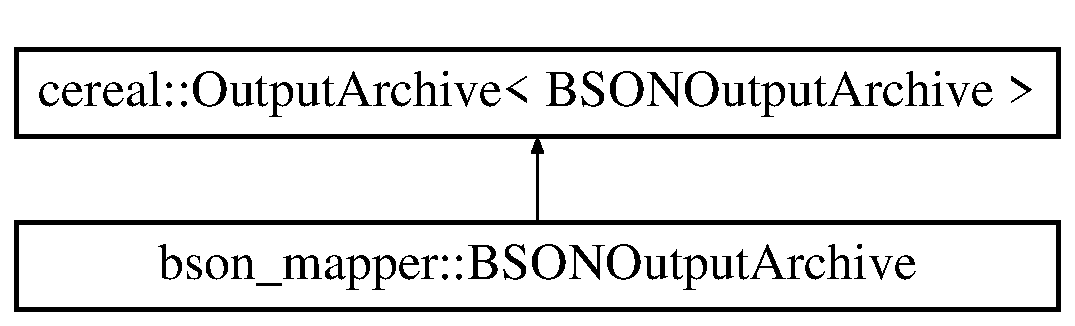
\includegraphics[height=2.000000cm]{classbson__mapper_1_1BSONOutputArchive}
\end{center}
\end{figure}
\subsection*{Public Member Functions}
\begin{DoxyCompactItemize}
\item 
\hyperlink{classbson__mapper_1_1BSONOutputArchive_a07af9bf8f5a9fa281c6424bfe39f453f}{B\+S\+O\+N\+Output\+Archive} (std\+::ostream \&stream, bool dot\+Notation\+Mode=false)
\begin{DoxyCompactList}\small\item\em Construct a \hyperlink{classbson__mapper_1_1BSONOutputArchive}{B\+S\+O\+N\+Output\+Archive} that will output serialized classes as B\+S\+ON to the provided stream. \end{DoxyCompactList}\end{DoxyCompactItemize}


\subsection{Constructor \& Destructor Documentation}
\index{bson\+\_\+mapper\+::\+B\+S\+O\+N\+Output\+Archive@{bson\+\_\+mapper\+::\+B\+S\+O\+N\+Output\+Archive}!B\+S\+O\+N\+Output\+Archive@{B\+S\+O\+N\+Output\+Archive}}
\index{B\+S\+O\+N\+Output\+Archive@{B\+S\+O\+N\+Output\+Archive}!bson\+\_\+mapper\+::\+B\+S\+O\+N\+Output\+Archive@{bson\+\_\+mapper\+::\+B\+S\+O\+N\+Output\+Archive}}
\subsubsection[{\texorpdfstring{B\+S\+O\+N\+Output\+Archive(std\+::ostream \&stream, bool dot\+Notation\+Mode=false)}{BSONOutputArchive(std::ostream &stream, bool dotNotationMode=false)}}]{\setlength{\rightskip}{0pt plus 5cm}bson\+\_\+mapper\+::\+B\+S\+O\+N\+Output\+Archive\+::\+B\+S\+O\+N\+Output\+Archive (
\begin{DoxyParamCaption}
\item[{std\+::ostream \&}]{stream, }
\item[{bool}]{dot\+Notation\+Mode = {\ttfamily false}}
\end{DoxyParamCaption}
)\hspace{0.3cm}{\ttfamily [inline]}}\hypertarget{classbson__mapper_1_1BSONOutputArchive_a07af9bf8f5a9fa281c6424bfe39f453f}{}\label{classbson__mapper_1_1BSONOutputArchive_a07af9bf8f5a9fa281c6424bfe39f453f}


Construct a \hyperlink{classbson__mapper_1_1BSONOutputArchive}{B\+S\+O\+N\+Output\+Archive} that will output serialized classes as B\+S\+ON to the provided stream. 


\begin{DoxyParams}{Parameters}
{\em stream} & The stream to which the archiver will output B\+S\+ON data.\\
\hline
{\em dot\+Notation\+Mode} & If set to true, the \hyperlink{classbson__mapper_1_1BSONOutputArchive}{B\+S\+O\+N\+Output\+Archive} will output the values in embedded documents in dot notation. This is useful when specifying the arguments to a \$set field in a Mongo\+DB update command.\\
\hline
\end{DoxyParams}
\begin{DoxySeeAlso}{See also}
\href{https://docs.mongodb.com/manual/core/document/#embedded-documents}{\tt https\+://docs.\+mongodb.\+com/manual/core/document/\#embedded-\/documents}
\end{DoxySeeAlso}
\begin{DoxyWarning}{Warning}
Documents produced by the archiver in dot\+Notation\+Mode are not compatible with the B\+S\+O\+N\+Input\+Archiver and are only intended to be used as a way to produce the argument to \$set. 
\end{DoxyWarning}


The documentation for this class was generated from the following file\+:\begin{DoxyCompactItemize}
\item 
src/bson\+\_\+mapper/bson\+\_\+archiver.\+hpp\end{DoxyCompactItemize}

\hypertarget{classbson__mapper_1_1char__array__streambuf}{}\section{bson\+\_\+mapper\+:\+:char\+\_\+array\+\_\+streambuf Class Reference}
\label{classbson__mapper_1_1char__array__streambuf}\index{bson\+\_\+mapper\+::char\+\_\+array\+\_\+streambuf@{bson\+\_\+mapper\+::char\+\_\+array\+\_\+streambuf}}


An input streambuf that uses an existing byte array as a buffer.  




{\ttfamily \#include $<$bson\+\_\+streambuf.\+hpp$>$}

Inheritance diagram for bson\+\_\+mapper\+:\+:char\+\_\+array\+\_\+streambuf\+:\begin{figure}[H]
\begin{center}
\leavevmode
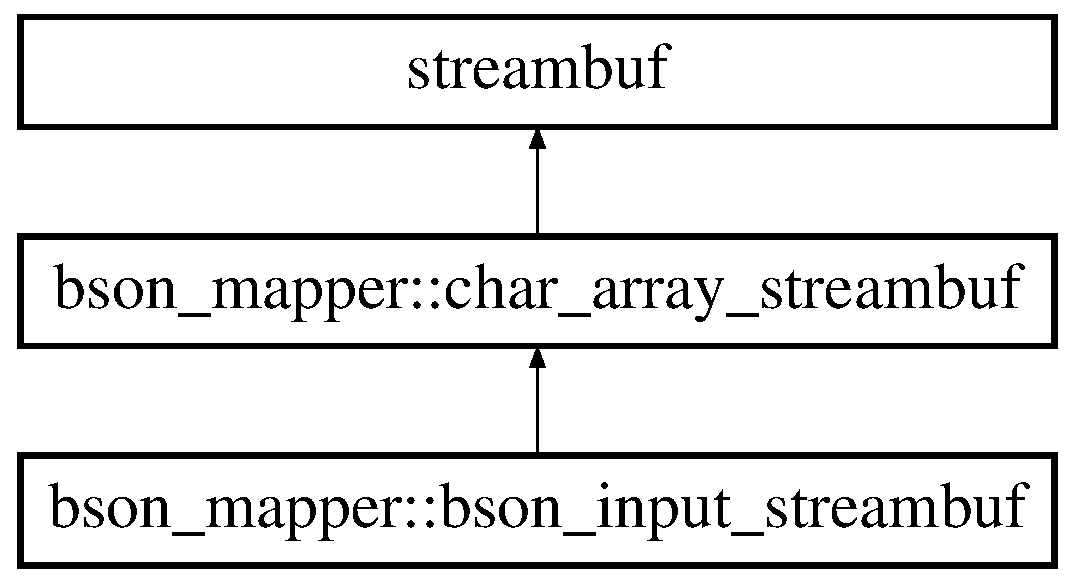
\includegraphics[height=3.000000cm]{classbson__mapper_1_1char__array__streambuf}
\end{center}
\end{figure}
\subsection*{Public Member Functions}
\begin{DoxyCompactItemize}
\item 
\hyperlink{classbson__mapper_1_1char__array__streambuf_a5cba6b0b5b8fab77b956375b4f8f9355}{char\+\_\+array\+\_\+streambuf} (const char $\ast$data, size\+\_\+t len)
\begin{DoxyCompactList}\small\item\em Create a streambuf around the given byte array. \end{DoxyCompactList}\end{DoxyCompactItemize}


\subsection{Detailed Description}
An input streambuf that uses an existing byte array as a buffer. 

\subsection{Constructor \& Destructor Documentation}
\index{bson\+\_\+mapper\+::char\+\_\+array\+\_\+streambuf@{bson\+\_\+mapper\+::char\+\_\+array\+\_\+streambuf}!char\+\_\+array\+\_\+streambuf@{char\+\_\+array\+\_\+streambuf}}
\index{char\+\_\+array\+\_\+streambuf@{char\+\_\+array\+\_\+streambuf}!bson\+\_\+mapper\+::char\+\_\+array\+\_\+streambuf@{bson\+\_\+mapper\+::char\+\_\+array\+\_\+streambuf}}
\subsubsection[{\texorpdfstring{char\+\_\+array\+\_\+streambuf(const char $\ast$data, size\+\_\+t len)}{char_array_streambuf(const char *data, size_t len)}}]{\setlength{\rightskip}{0pt plus 5cm}bson\+\_\+mapper\+::char\+\_\+array\+\_\+streambuf\+::char\+\_\+array\+\_\+streambuf (
\begin{DoxyParamCaption}
\item[{const char $\ast$}]{data, }
\item[{size\+\_\+t}]{len}
\end{DoxyParamCaption}
)}\hypertarget{classbson__mapper_1_1char__array__streambuf_a5cba6b0b5b8fab77b956375b4f8f9355}{}\label{classbson__mapper_1_1char__array__streambuf_a5cba6b0b5b8fab77b956375b4f8f9355}


Create a streambuf around the given byte array. 

The caller is responsible for maintaining the lifetime of the underlying data. 
\begin{DoxyParams}{Parameters}
{\em data} & A pointer to the data to be read \\
\hline
{\em len} & The length of the data \\
\hline
\end{DoxyParams}


The documentation for this class was generated from the following file\+:\begin{DoxyCompactItemize}
\item 
src/bson\+\_\+mapper/bson\+\_\+streambuf.\+hpp\end{DoxyCompactItemize}

\hypertarget{classmongo__odm_1_1comparison__expr}{}\section{mongo\+\_\+odm\+:\+:comparison\+\_\+expr$<$ NvpT, U $>$ Class Template Reference}
\label{classmongo__odm_1_1comparison__expr}\index{mongo\+\_\+odm\+::comparison\+\_\+expr$<$ Nvp\+T, U $>$@{mongo\+\_\+odm\+::comparison\+\_\+expr$<$ Nvp\+T, U $>$}}


Represents a query expression with the syntax \char`\"{}key\+: \{\$op\+: value\}\char`\"{}.  




{\ttfamily \#include $<$query\+\_\+builder.\+hpp$>$}

Inheritance diagram for mongo\+\_\+odm\+:\+:comparison\+\_\+expr$<$ NvpT, U $>$\+:\begin{figure}[H]
\begin{center}
\leavevmode
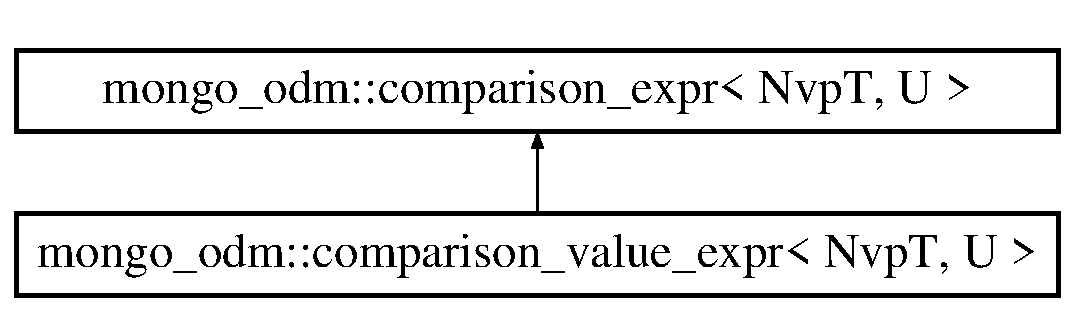
\includegraphics[height=2.000000cm]{classmongo__odm_1_1comparison__expr}
\end{center}
\end{figure}
\subsection*{Public Member Functions}
\begin{DoxyCompactItemize}
\item 
constexpr \hyperlink{classmongo__odm_1_1comparison__expr_a8cb08d386b0b1cbb88780d12c29c385e}{comparison\+\_\+expr} (const NvpT \&\hyperlink{classmongo__odm_1_1nvp}{nvp}, const U \&field, const char $\ast$op)
\begin{DoxyCompactList}\small\item\em Constructs a query expression for the given key, value, and comparison type. \end{DoxyCompactList}\item 
constexpr \hyperlink{classmongo__odm_1_1comparison__expr_aa60e06beaf4e99b7b73a445b4fc5ffe7}{comparison\+\_\+expr} (const \hyperlink{classmongo__odm_1_1comparison__expr}{comparison\+\_\+expr} \&expr, const char $\ast$op)
\begin{DoxyCompactList}\small\item\em Takes a comparison expression, and creates a new one with a different operator, but the same value and field. \end{DoxyCompactList}\item 
std\+::string \& \hyperlink{classmongo__odm_1_1comparison__expr_a3adf1fd565c8a6c1bb01ca9d4ee42ce5}{append\+\_\+name} (std\+::string \&s) const \hypertarget{classmongo__odm_1_1comparison__expr_a3adf1fd565c8a6c1bb01ca9d4ee42ce5}{}\label{classmongo__odm_1_1comparison__expr_a3adf1fd565c8a6c1bb01ca9d4ee42ce5}

\begin{DoxyCompactList}\small\item\em Appends the name of the contained field to a string. \end{DoxyCompactList}\item 
void \hyperlink{classmongo__odm_1_1comparison__expr_a2ed6e4e5fd013703369938911b4c367e}{append\+\_\+to\+\_\+bson} (bsoncxx\+::builder\+::core \&builder, bool wrap=false, bool omit\+\_\+name=false) const 
\begin{DoxyCompactList}\small\item\em Appends this expression to a B\+S\+ON core builder, as a key-\/value pair of the form \char`\"{}key\+: \{\$cmp\+: val\}\char`\"{}, where \$cmp is some comparison operator. \end{DoxyCompactList}\item 
\hyperlink{classmongo__odm_1_1comparison__expr_a5c3c4afa7894a5268e6c9ab76c4d83e3}{operator bsoncxx\+::document\+::view\+\_\+or\+\_\+value} () const 
\begin{DoxyCompactList}\small\item\em Converts the expression to a B\+S\+ON filter for a query. \end{DoxyCompactList}\end{DoxyCompactItemize}


\subsection{Detailed Description}
\subsubsection*{template$<$typename NvpT, typename U$>$\\*
class mongo\+\_\+odm\+::comparison\+\_\+expr$<$ Nvp\+T, U $>$}

Represents a query expression with the syntax \char`\"{}key\+: \{\$op\+: value\}\char`\"{}. 

This usually means queries that are comparisons, such as (User.\+age $>$ 21). However, this also covers operators such as \$exists, or any operator that has the above syntax. 
\begin{DoxyTemplParams}{Template Parameters}
{\em NvpT} & The type of the name-\/value pair this expression uses. \\
\hline
{\em U} & The type of the value to compare against. This could be the same as the value type of NvpT, or the type of some other parameter, or even a query builder expression. \\
\hline
\end{DoxyTemplParams}


\subsection{Constructor \& Destructor Documentation}
\index{mongo\+\_\+odm\+::comparison\+\_\+expr@{mongo\+\_\+odm\+::comparison\+\_\+expr}!comparison\+\_\+expr@{comparison\+\_\+expr}}
\index{comparison\+\_\+expr@{comparison\+\_\+expr}!mongo\+\_\+odm\+::comparison\+\_\+expr@{mongo\+\_\+odm\+::comparison\+\_\+expr}}
\subsubsection[{\texorpdfstring{comparison\+\_\+expr(const Nvp\+T \&nvp, const U \&field, const char $\ast$op)}{comparison_expr(const NvpT &nvp, const U &field, const char *op)}}]{\setlength{\rightskip}{0pt plus 5cm}template$<$typename NvpT, typename U$>$ constexpr {\bf mongo\+\_\+odm\+::comparison\+\_\+expr}$<$ NvpT, U $>$\+::{\bf comparison\+\_\+expr} (
\begin{DoxyParamCaption}
\item[{const NvpT \&}]{nvp, }
\item[{const U \&}]{field, }
\item[{const char $\ast$}]{op}
\end{DoxyParamCaption}
)\hspace{0.3cm}{\ttfamily [inline]}}\hypertarget{classmongo__odm_1_1comparison__expr_a8cb08d386b0b1cbb88780d12c29c385e}{}\label{classmongo__odm_1_1comparison__expr_a8cb08d386b0b1cbb88780d12c29c385e}


Constructs a query expression for the given key, value, and comparison type. 


\begin{DoxyParams}{Parameters}
{\em nvp} & A name-\/value pair corresponding to a key in a document \\
\hline
{\em field} & The value that the key is being compared to. \\
\hline
{\em op} & The type of comparison operator, such at gt ($>$) or ne (!=). \\
\hline
\end{DoxyParams}
\index{mongo\+\_\+odm\+::comparison\+\_\+expr@{mongo\+\_\+odm\+::comparison\+\_\+expr}!comparison\+\_\+expr@{comparison\+\_\+expr}}
\index{comparison\+\_\+expr@{comparison\+\_\+expr}!mongo\+\_\+odm\+::comparison\+\_\+expr@{mongo\+\_\+odm\+::comparison\+\_\+expr}}
\subsubsection[{\texorpdfstring{comparison\+\_\+expr(const comparison\+\_\+expr \&expr, const char $\ast$op)}{comparison_expr(const comparison_expr &expr, const char *op)}}]{\setlength{\rightskip}{0pt plus 5cm}template$<$typename NvpT, typename U$>$ constexpr {\bf mongo\+\_\+odm\+::comparison\+\_\+expr}$<$ NvpT, U $>$\+::{\bf comparison\+\_\+expr} (
\begin{DoxyParamCaption}
\item[{const {\bf comparison\+\_\+expr}$<$ NvpT, U $>$ \&}]{expr, }
\item[{const char $\ast$}]{op}
\end{DoxyParamCaption}
)\hspace{0.3cm}{\ttfamily [inline]}}\hypertarget{classmongo__odm_1_1comparison__expr_aa60e06beaf4e99b7b73a445b4fc5ffe7}{}\label{classmongo__odm_1_1comparison__expr_aa60e06beaf4e99b7b73a445b4fc5ffe7}


Takes a comparison expression, and creates a new one with a different operator, but the same value and field. 

This is primarily used to wrap \$regex operators in \$not, since \$not cannot contains a \$regex operator, it must directly contain the regex itself. 
\begin{DoxyParams}{Parameters}
{\em expr} & A comparison expresison with a similar field type and value type. \\
\hline
{\em op} & The new operator to use. \\
\hline
\end{DoxyParams}


\subsection{Member Function Documentation}
\index{mongo\+\_\+odm\+::comparison\+\_\+expr@{mongo\+\_\+odm\+::comparison\+\_\+expr}!append\+\_\+to\+\_\+bson@{append\+\_\+to\+\_\+bson}}
\index{append\+\_\+to\+\_\+bson@{append\+\_\+to\+\_\+bson}!mongo\+\_\+odm\+::comparison\+\_\+expr@{mongo\+\_\+odm\+::comparison\+\_\+expr}}
\subsubsection[{\texorpdfstring{append\+\_\+to\+\_\+bson(bsoncxx\+::builder\+::core \&builder, bool wrap=false, bool omit\+\_\+name=false) const }{append_to_bson(bsoncxx::builder::core &builder, bool wrap=false, bool omit_name=false) const }}]{\setlength{\rightskip}{0pt plus 5cm}template$<$typename NvpT, typename U$>$ void {\bf mongo\+\_\+odm\+::comparison\+\_\+expr}$<$ NvpT, U $>$\+::append\+\_\+to\+\_\+bson (
\begin{DoxyParamCaption}
\item[{bsoncxx\+::builder\+::core \&}]{builder, }
\item[{bool}]{wrap = {\ttfamily false}, }
\item[{bool}]{omit\+\_\+name = {\ttfamily false}}
\end{DoxyParamCaption}
) const\hspace{0.3cm}{\ttfamily [inline]}}\hypertarget{classmongo__odm_1_1comparison__expr_a2ed6e4e5fd013703369938911b4c367e}{}\label{classmongo__odm_1_1comparison__expr_a2ed6e4e5fd013703369938911b4c367e}


Appends this expression to a B\+S\+ON core builder, as a key-\/value pair of the form \char`\"{}key\+: \{\$cmp\+: val\}\char`\"{}, where \$cmp is some comparison operator. 


\begin{DoxyParams}{Parameters}
{\em builder} & A B\+S\+ON core builder \\
\hline
{\em wrap} & Whether to wrap the B\+S\+ON inside a document. \\
\hline
{\em omit\+\_\+name} & Whether to skip the name of the field. This is used primarily in \hyperlink{classmongo__odm_1_1not__expr}{not\+\_\+expr} and free\+\_\+expr to append just the value of the expression. \\
\hline
\end{DoxyParams}
\index{mongo\+\_\+odm\+::comparison\+\_\+expr@{mongo\+\_\+odm\+::comparison\+\_\+expr}!operator bsoncxx\+::document\+::view\+\_\+or\+\_\+value@{operator bsoncxx\+::document\+::view\+\_\+or\+\_\+value}}
\index{operator bsoncxx\+::document\+::view\+\_\+or\+\_\+value@{operator bsoncxx\+::document\+::view\+\_\+or\+\_\+value}!mongo\+\_\+odm\+::comparison\+\_\+expr@{mongo\+\_\+odm\+::comparison\+\_\+expr}}
\subsubsection[{\texorpdfstring{operator bsoncxx\+::document\+::view\+\_\+or\+\_\+value() const }{operator bsoncxx::document::view_or_value() const }}]{\setlength{\rightskip}{0pt plus 5cm}template$<$typename NvpT, typename U$>$ {\bf mongo\+\_\+odm\+::comparison\+\_\+expr}$<$ NvpT, U $>$\+::operator bsoncxx\+::document\+::view\+\_\+or\+\_\+value (
\begin{DoxyParamCaption}
{}
\end{DoxyParamCaption}
) const\hspace{0.3cm}{\ttfamily [inline]}}\hypertarget{classmongo__odm_1_1comparison__expr_a5c3c4afa7894a5268e6c9ab76c4d83e3}{}\label{classmongo__odm_1_1comparison__expr_a5c3c4afa7894a5268e6c9ab76c4d83e3}


Converts the expression to a B\+S\+ON filter for a query. 

The format of the B\+S\+ON is \char`\"{}\{key\+: \{\$not\+: \{\$cmp\+: val\}\}\}\char`\"{}. 

The documentation for this class was generated from the following files\+:\begin{DoxyCompactItemize}
\item 
src/mongo\+\_\+odm/expression\+\_\+syntax.\+hpp\item 
src/mongo\+\_\+odm/query\+\_\+builder.\+hpp\end{DoxyCompactItemize}

\hypertarget{classmongo__odm_1_1comparison__value__expr}{}\section{mongo\+\_\+odm\+:\+:comparison\+\_\+value\+\_\+expr$<$ NvpT, U $>$ Class Template Reference}
\label{classmongo__odm_1_1comparison__value__expr}\index{mongo\+\_\+odm\+::comparison\+\_\+value\+\_\+expr$<$ Nvp\+T, U $>$@{mongo\+\_\+odm\+::comparison\+\_\+value\+\_\+expr$<$ Nvp\+T, U $>$}}


Represents a comparison expression as above, but stores a value instead of a reference.  




{\ttfamily \#include $<$query\+\_\+builder.\+hpp$>$}

Inheritance diagram for mongo\+\_\+odm\+:\+:comparison\+\_\+value\+\_\+expr$<$ NvpT, U $>$\+:\begin{figure}[H]
\begin{center}
\leavevmode
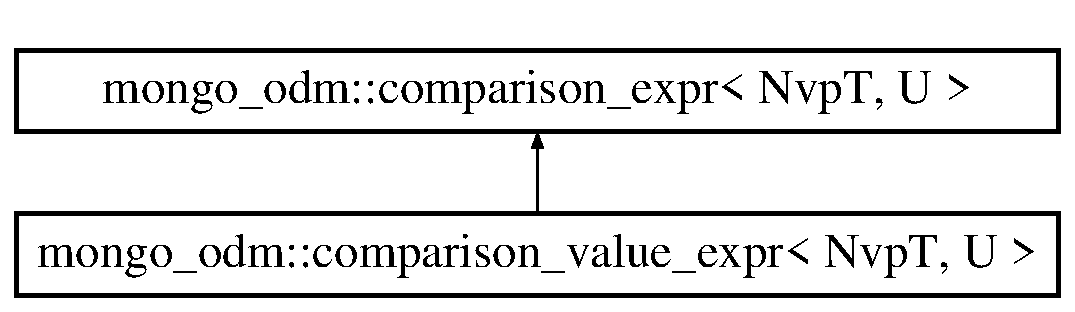
\includegraphics[height=2.000000cm]{classmongo__odm_1_1comparison__value__expr}
\end{center}
\end{figure}
\subsection*{Additional Inherited Members}


\subsection{Detailed Description}
\subsubsection*{template$<$typename NvpT, typename U$>$\\*
class mongo\+\_\+odm\+::comparison\+\_\+value\+\_\+expr$<$ Nvp\+T, U $>$}

Represents a comparison expression as above, but stores a value instead of a reference. 

This is useful for storing temporary or computed values. Internally, it uses a \hyperlink{classmongo__odm_1_1comparison__expr}{comparison\+\_\+expr} whose value is a b\+\_\+regex. 

The documentation for this class was generated from the following files\+:\begin{DoxyCompactItemize}
\item 
src/mongo\+\_\+odm/expression\+\_\+syntax.\+hpp\item 
src/mongo\+\_\+odm/query\+\_\+builder.\+hpp\end{DoxyCompactItemize}

\hypertarget{classmongo__odm_1_1current__date__expr}{}\section{mongo\+\_\+odm\+:\+:current\+\_\+date\+\_\+expr$<$ NvpT $>$ Class Template Reference}
\label{classmongo__odm_1_1current__date__expr}\index{mongo\+\_\+odm\+::current\+\_\+date\+\_\+expr$<$ Nvp\+T $>$@{mongo\+\_\+odm\+::current\+\_\+date\+\_\+expr$<$ Nvp\+T $>$}}


Creates an expression that uses the \$current\+Date operator.  




{\ttfamily \#include $<$query\+\_\+builder.\+hpp$>$}

\subsection*{Public Member Functions}
\begin{DoxyCompactItemize}
\item 
constexpr \hyperlink{classmongo__odm_1_1current__date__expr_a1d4c6659a44bc917bbf908a2011ff3d4}{current\+\_\+date\+\_\+expr} (const NvpT \&\hyperlink{classmongo__odm_1_1nvp}{nvp}, bool \hyperlink{structmongo__odm_1_1is__date}{is\+\_\+date})
\begin{DoxyCompactList}\small\item\em Creates an expression that uses the \$current\+Date operator with a given field and type. \end{DoxyCompactList}\item 
void \hyperlink{classmongo__odm_1_1current__date__expr_aa53602f8d005cd22150b0482c4f2070d}{append\+\_\+to\+\_\+bson} (bsoncxx\+::builder\+::core \&builder, bool wrap=false) const 
\begin{DoxyCompactList}\small\item\em Appends this query to a B\+S\+ON core builder as an expression \textquotesingle{}. \end{DoxyCompactList}\end{DoxyCompactItemize}


\subsection{Detailed Description}
\subsubsection*{template$<$typename NvpT$>$\\*
class mongo\+\_\+odm\+::current\+\_\+date\+\_\+expr$<$ Nvp\+T $>$}

Creates an expression that uses the \$current\+Date operator. 

\subsection{Constructor \& Destructor Documentation}
\index{mongo\+\_\+odm\+::current\+\_\+date\+\_\+expr@{mongo\+\_\+odm\+::current\+\_\+date\+\_\+expr}!current\+\_\+date\+\_\+expr@{current\+\_\+date\+\_\+expr}}
\index{current\+\_\+date\+\_\+expr@{current\+\_\+date\+\_\+expr}!mongo\+\_\+odm\+::current\+\_\+date\+\_\+expr@{mongo\+\_\+odm\+::current\+\_\+date\+\_\+expr}}
\subsubsection[{\texorpdfstring{current\+\_\+date\+\_\+expr(const Nvp\+T \&nvp, bool is\+\_\+date)}{current_date_expr(const NvpT &nvp, bool is_date)}}]{\setlength{\rightskip}{0pt plus 5cm}template$<$typename NvpT $>$ constexpr {\bf mongo\+\_\+odm\+::current\+\_\+date\+\_\+expr}$<$ NvpT $>$\+::{\bf current\+\_\+date\+\_\+expr} (
\begin{DoxyParamCaption}
\item[{const NvpT \&}]{nvp, }
\item[{bool}]{is\+\_\+date}
\end{DoxyParamCaption}
)\hspace{0.3cm}{\ttfamily [inline]}}\hypertarget{classmongo__odm_1_1current__date__expr_a1d4c6659a44bc917bbf908a2011ff3d4}{}\label{classmongo__odm_1_1current__date__expr_a1d4c6659a44bc917bbf908a2011ff3d4}


Creates an expression that uses the \$current\+Date operator with a given field and type. 


\begin{DoxyParams}{Parameters}
{\em nvp} & The given field \\
\hline
{\em \hyperlink{structmongo__odm_1_1is__date}{is\+\_\+date}} & Whether the field\textquotesingle{}s type is a date (true) or a timestmap (false) \\
\hline
\end{DoxyParams}


\subsection{Member Function Documentation}
\index{mongo\+\_\+odm\+::current\+\_\+date\+\_\+expr@{mongo\+\_\+odm\+::current\+\_\+date\+\_\+expr}!append\+\_\+to\+\_\+bson@{append\+\_\+to\+\_\+bson}}
\index{append\+\_\+to\+\_\+bson@{append\+\_\+to\+\_\+bson}!mongo\+\_\+odm\+::current\+\_\+date\+\_\+expr@{mongo\+\_\+odm\+::current\+\_\+date\+\_\+expr}}
\subsubsection[{\texorpdfstring{append\+\_\+to\+\_\+bson(bsoncxx\+::builder\+::core \&builder, bool wrap=false) const }{append_to_bson(bsoncxx::builder::core &builder, bool wrap=false) const }}]{\setlength{\rightskip}{0pt plus 5cm}template$<$typename NvpT $>$ void {\bf mongo\+\_\+odm\+::current\+\_\+date\+\_\+expr}$<$ NvpT $>$\+::append\+\_\+to\+\_\+bson (
\begin{DoxyParamCaption}
\item[{bsoncxx\+::builder\+::core \&}]{builder, }
\item[{bool}]{wrap = {\ttfamily false}}
\end{DoxyParamCaption}
) const\hspace{0.3cm}{\ttfamily [inline]}}\hypertarget{classmongo__odm_1_1current__date__expr_aa53602f8d005cd22150b0482c4f2070d}{}\label{classmongo__odm_1_1current__date__expr_aa53602f8d005cd22150b0482c4f2070d}


Appends this query to a B\+S\+ON core builder as an expression \textquotesingle{}. 

\begin{DoxyParagraph}{current\+Date}
\{field\+: \{
\end{DoxyParagraph}
type\+: \char`\"{}timestamp$\vert$date\char`\"{}\}\}\textquotesingle{} 
\begin{DoxyParams}{Parameters}
{\em builder} & A basic B\+S\+ON core builder. \\
\hline
{\em Whether} & to wrap this expression inside a document. \\
\hline
\end{DoxyParams}


The documentation for this class was generated from the following files\+:\begin{DoxyCompactItemize}
\item 
src/mongo\+\_\+odm/expression\+\_\+syntax.\+hpp\item 
src/mongo\+\_\+odm/query\+\_\+builder.\+hpp\end{DoxyCompactItemize}

\hypertarget{structmongo__odm_1_1current__date__t}{}\section{mongo\+\_\+odm\+:\+:current\+\_\+date\+\_\+t Struct Reference}
\label{structmongo__odm_1_1current__date__t}\index{mongo\+\_\+odm\+::current\+\_\+date\+\_\+t@{mongo\+\_\+odm\+::current\+\_\+date\+\_\+t}}


The documentation for this struct was generated from the following file\+:\begin{DoxyCompactItemize}
\item 
src/mongo\+\_\+odm/nvp.\+hpp\end{DoxyCompactItemize}

\hypertarget{classmongo__odm_1_1deserializing__cursor}{}\section{mongo\+\_\+odm\+:\+:deserializing\+\_\+cursor$<$ T $>$ Class Template Reference}
\label{classmongo__odm_1_1deserializing__cursor}\index{mongo\+\_\+odm\+::deserializing\+\_\+cursor$<$ T $>$@{mongo\+\_\+odm\+::deserializing\+\_\+cursor$<$ T $>$}}


A class that wraps a mongocxx\+::cursor.  




{\ttfamily \#include $<$deserializing\+\_\+cursor.\+hpp$>$}

\subsection*{Classes}
\begin{DoxyCompactItemize}
\item 
class \hyperlink{classmongo__odm_1_1deserializing__cursor_1_1iterator}{iterator}
\end{DoxyCompactItemize}


\subsection{Detailed Description}
\subsubsection*{template$<$class T$>$\\*
class mongo\+\_\+odm\+::deserializing\+\_\+cursor$<$ T $>$}

A class that wraps a mongocxx\+::cursor. 

It provides an iterator that deserializes the documents yielded by the underlying mongocxx cursor. N\+O\+TE\+: This iterator will skip documents that fail to be deserialized, e.\+g. due to non-\/matching schemas. 

The documentation for this class was generated from the following file\+:\begin{DoxyCompactItemize}
\item 
src/mongo\+\_\+odm/deserializing\+\_\+cursor.\+hpp\end{DoxyCompactItemize}

\hypertarget{classmongo__odm_1_1dollar__operator__nvp}{}\section{mongo\+\_\+odm\+:\+:dollar\+\_\+operator\+\_\+nvp$<$ NvpT $>$ Class Template Reference}
\label{classmongo__odm_1_1dollar__operator__nvp}\index{mongo\+\_\+odm\+::dollar\+\_\+operator\+\_\+nvp$<$ Nvp\+T $>$@{mongo\+\_\+odm\+::dollar\+\_\+operator\+\_\+nvp$<$ Nvp\+T $>$}}


Represents the \$ operator applied to a field.  




{\ttfamily \#include $<$nvp.\+hpp$>$}

Inheritance diagram for mongo\+\_\+odm\+:\+:dollar\+\_\+operator\+\_\+nvp$<$ NvpT $>$\+:\begin{figure}[H]
\begin{center}
\leavevmode
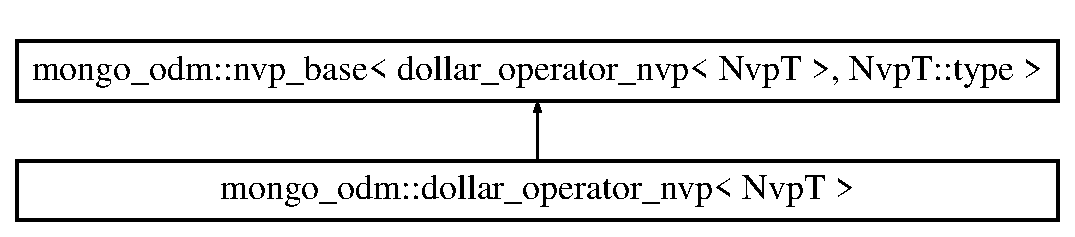
\includegraphics[height=2.000000cm]{classmongo__odm_1_1dollar__operator__nvp}
\end{center}
\end{figure}
\subsection*{Public Member Functions}
\begin{DoxyCompactItemize}
\item 
constexpr \hyperlink{classmongo__odm_1_1update__expr}{update\+\_\+expr}$<$ \hyperlink{classmongo__odm_1_1dollar__operator__nvp}{dollar\+\_\+operator\+\_\+nvp}$<$ NvpT $>$, no\+\_\+opt\+\_\+type $>$ \hyperlink{classmongo__odm_1_1dollar__operator__nvp_a09553e7ffa1350ae96b53b0050c83d45}{operator=} (const no\+\_\+opt\+\_\+type \&val) const \hypertarget{classmongo__odm_1_1dollar__operator__nvp_a09553e7ffa1350ae96b53b0050c83d45}{}\label{classmongo__odm_1_1dollar__operator__nvp_a09553e7ffa1350ae96b53b0050c83d45}

\begin{DoxyCompactList}\small\item\em Creates an update expression that sets the field to the given value. \end{DoxyCompactList}\item 
std\+::string \hyperlink{classmongo__odm_1_1dollar__operator__nvp_a4ccad25d5b45c435cf3600826eed9315}{get\+\_\+name} () const 
\begin{DoxyCompactList}\small\item\em Returns the qualified name of this field in dot notation, i.\+e. \end{DoxyCompactList}\item 
std\+::string \& \hyperlink{classmongo__odm_1_1dollar__operator__nvp_af61ffed690dde76d535d3bda787711ad}{append\+\_\+name} (std\+::string \&s) const 
\begin{DoxyCompactList}\small\item\em Returns the name of this field with the \$ operator, i.\+e. \end{DoxyCompactList}\end{DoxyCompactItemize}


\subsection{Detailed Description}
\subsubsection*{template$<$typename NvpT$>$\\*
class mongo\+\_\+odm\+::dollar\+\_\+operator\+\_\+nvp$<$ Nvp\+T $>$}

Represents the \$ operator applied to a field. 

\subsection{Member Function Documentation}
\index{mongo\+\_\+odm\+::dollar\+\_\+operator\+\_\+nvp@{mongo\+\_\+odm\+::dollar\+\_\+operator\+\_\+nvp}!append\+\_\+name@{append\+\_\+name}}
\index{append\+\_\+name@{append\+\_\+name}!mongo\+\_\+odm\+::dollar\+\_\+operator\+\_\+nvp@{mongo\+\_\+odm\+::dollar\+\_\+operator\+\_\+nvp}}
\subsubsection[{\texorpdfstring{append\+\_\+name(std\+::string \&s) const }{append_name(std::string &s) const }}]{\setlength{\rightskip}{0pt plus 5cm}template$<$typename NvpT $>$ std\+::string\& {\bf mongo\+\_\+odm\+::dollar\+\_\+operator\+\_\+nvp}$<$ NvpT $>$\+::append\+\_\+name (
\begin{DoxyParamCaption}
\item[{std\+::string \&}]{s}
\end{DoxyParamCaption}
) const\hspace{0.3cm}{\ttfamily [inline]}}\hypertarget{classmongo__odm_1_1dollar__operator__nvp_af61ffed690dde76d535d3bda787711ad}{}\label{classmongo__odm_1_1dollar__operator__nvp_af61ffed690dde76d535d3bda787711ad}


Returns the name of this field with the \$ operator, i.\+e. 

\char`\"{}field.\$\char`\"{} \begin{DoxyReturn}{Returns}
A string containing the name of this field in dot notation. 
\end{DoxyReturn}
\index{mongo\+\_\+odm\+::dollar\+\_\+operator\+\_\+nvp@{mongo\+\_\+odm\+::dollar\+\_\+operator\+\_\+nvp}!get\+\_\+name@{get\+\_\+name}}
\index{get\+\_\+name@{get\+\_\+name}!mongo\+\_\+odm\+::dollar\+\_\+operator\+\_\+nvp@{mongo\+\_\+odm\+::dollar\+\_\+operator\+\_\+nvp}}
\subsubsection[{\texorpdfstring{get\+\_\+name() const }{get_name() const }}]{\setlength{\rightskip}{0pt plus 5cm}template$<$typename NvpT $>$ std\+::string {\bf mongo\+\_\+odm\+::dollar\+\_\+operator\+\_\+nvp}$<$ NvpT $>$\+::get\+\_\+name (
\begin{DoxyParamCaption}
{}
\end{DoxyParamCaption}
) const\hspace{0.3cm}{\ttfamily [inline]}}\hypertarget{classmongo__odm_1_1dollar__operator__nvp_a4ccad25d5b45c435cf3600826eed9315}{}\label{classmongo__odm_1_1dollar__operator__nvp_a4ccad25d5b45c435cf3600826eed9315}


Returns the qualified name of this field in dot notation, i.\+e. 

\char`\"{}array.\+i\char`\"{}. \begin{DoxyReturn}{Returns}
A string containing the name of this field in dot notation. 
\end{DoxyReturn}


The documentation for this class was generated from the following file\+:\begin{DoxyCompactItemize}
\item 
src/mongo\+\_\+odm/nvp.\+hpp\end{DoxyCompactItemize}

\hypertarget{structbson__mapper_1_1Exception}{}\section{bson\+\_\+mapper\+:\+:Exception Struct Reference}
\label{structbson__mapper_1_1Exception}\index{bson\+\_\+mapper\+::\+Exception@{bson\+\_\+mapper\+::\+Exception}}


An exception class thrown when things go wrong at runtime.  




{\ttfamily \#include $<$bson\+\_\+archiver.\+hpp$>$}

Inheritance diagram for bson\+\_\+mapper\+:\+:Exception\+:\begin{figure}[H]
\begin{center}
\leavevmode
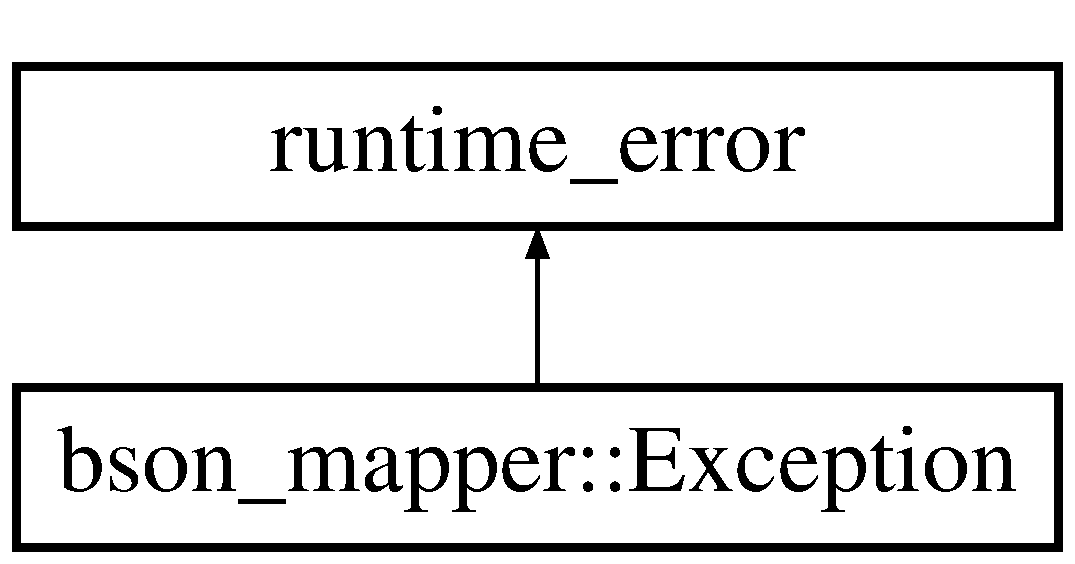
\includegraphics[height=2.000000cm]{structbson__mapper_1_1Exception}
\end{center}
\end{figure}


\subsection{Detailed Description}
An exception class thrown when things go wrong at runtime. 

The documentation for this struct was generated from the following file\+:\begin{DoxyCompactItemize}
\item 
src/bson\+\_\+mapper/bson\+\_\+archiver.\+hpp\end{DoxyCompactItemize}

\hypertarget{structmongo__odm_1_1expression__category__t}{}\section{mongo\+\_\+odm\+:\+:expression\+\_\+category\+\_\+t$<$ expr\+\_\+type $>$ Struct Template Reference}
\label{structmongo__odm_1_1expression__category__t}\index{mongo\+\_\+odm\+::expression\+\_\+category\+\_\+t$<$ expr\+\_\+type $>$@{mongo\+\_\+odm\+::expression\+\_\+category\+\_\+t$<$ expr\+\_\+type $>$}}
Inheritance diagram for mongo\+\_\+odm\+:\+:expression\+\_\+category\+\_\+t$<$ expr\+\_\+type $>$\+:\begin{figure}[H]
\begin{center}
\leavevmode
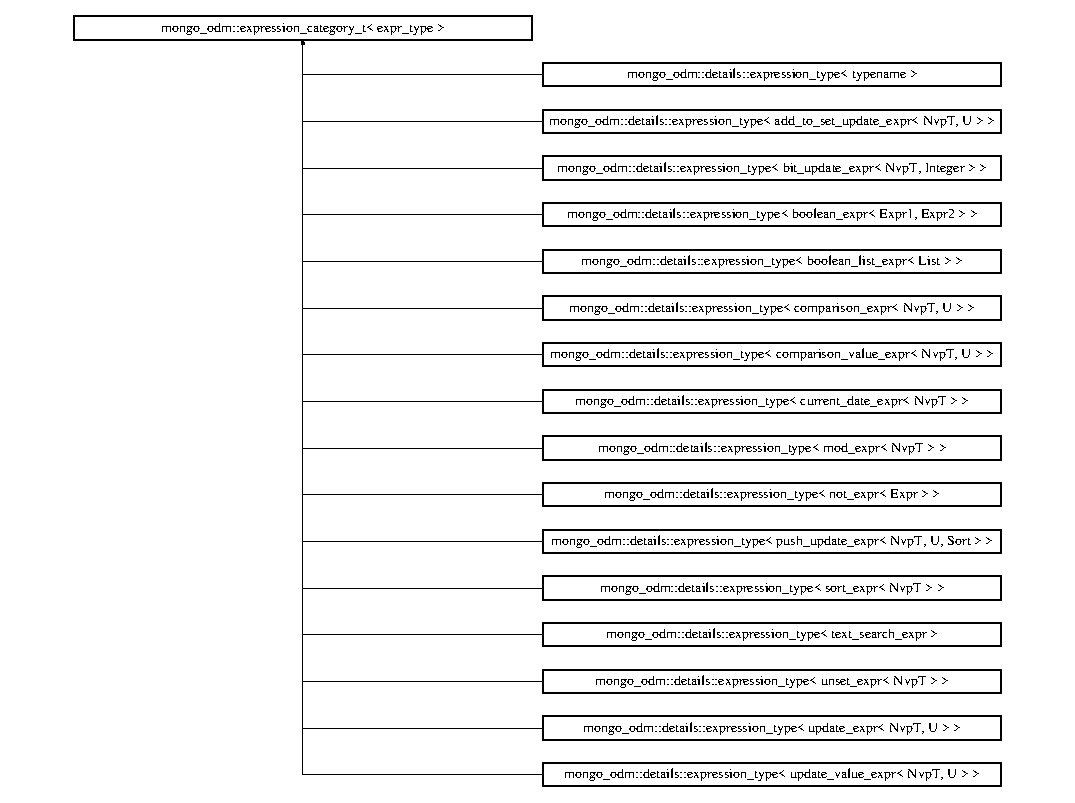
\includegraphics[height=10.347826cm]{structmongo__odm_1_1expression__category__t}
\end{center}
\end{figure}


The documentation for this struct was generated from the following file\+:\begin{DoxyCompactItemize}
\item 
src/mongo\+\_\+odm/expression\+\_\+syntax.\+hpp\end{DoxyCompactItemize}

\hypertarget{classmongo__odm_1_1expression__list}{}\section{mongo\+\_\+odm\+:\+:expression\+\_\+list$<$ list\+\_\+type, Args $>$ Class Template Reference}
\label{classmongo__odm_1_1expression__list}\index{mongo\+\_\+odm\+::expression\+\_\+list$<$ list\+\_\+type, Args $>$@{mongo\+\_\+odm\+::expression\+\_\+list$<$ list\+\_\+type, Args $>$}}


This represents a list of expressions.  




{\ttfamily \#include $<$query\+\_\+builder.\+hpp$>$}

\subsection*{Public Member Functions}
\begin{DoxyCompactItemize}
\item 
\hyperlink{classmongo__odm_1_1expression__list_a005746d6c92dc87c719a0e8029493590}{expression\+\_\+list} (const Args \&...args)
\begin{DoxyCompactList}\small\item\em Constructs an expression list of the given arguments. \end{DoxyCompactList}\item 
void \hyperlink{classmongo__odm_1_1expression__list_a85ac4de221b14cf6adf52945fd9f7507}{append\+\_\+to\+\_\+bson} (bsoncxx\+::builder\+::core \&builder, bool wrap=false) const 
\begin{DoxyCompactList}\small\item\em Appends each element to a B\+S\+ON code builder. \end{DoxyCompactList}\item 
\hyperlink{classmongo__odm_1_1expression__list_a210238378d08926cab580c63dec1a31c}{operator bsoncxx\+::document\+::view\+\_\+or\+\_\+value} () const 
\begin{DoxyCompactList}\small\item\em Casts the expression list to a B\+S\+ON query of the form \{ expr1, expr2, .... \end{DoxyCompactList}\end{DoxyCompactItemize}


\subsection{Detailed Description}
\subsubsection*{template$<$expression\+\_\+category list\+\_\+type, typename... Args$>$\\*
class mongo\+\_\+odm\+::expression\+\_\+list$<$ list\+\_\+type, Args $>$}

This represents a list of expressions. 


\begin{DoxyTemplParams}{Template Parameters}
{\em list\+\_\+type} & The category of the expressions, such as \char`\"{}update\char`\"{} or \char`\"{}query\char`\"{}. \\
\hline
{\em Args...} & The types of the various expressions that make up the list. \\
\hline
\end{DoxyTemplParams}


\subsection{Constructor \& Destructor Documentation}
\index{mongo\+\_\+odm\+::expression\+\_\+list@{mongo\+\_\+odm\+::expression\+\_\+list}!expression\+\_\+list@{expression\+\_\+list}}
\index{expression\+\_\+list@{expression\+\_\+list}!mongo\+\_\+odm\+::expression\+\_\+list@{mongo\+\_\+odm\+::expression\+\_\+list}}
\subsubsection[{\texorpdfstring{expression\+\_\+list(const Args \&...\+args)}{expression_list(const Args &...args)}}]{\setlength{\rightskip}{0pt plus 5cm}template$<$expression\+\_\+category list\+\_\+type, typename... Args$>$ {\bf mongo\+\_\+odm\+::expression\+\_\+list}$<$ list\+\_\+type, Args $>$\+::{\bf expression\+\_\+list} (
\begin{DoxyParamCaption}
\item[{const Args \&...}]{args}
\end{DoxyParamCaption}
)\hspace{0.3cm}{\ttfamily [inline]}}\hypertarget{classmongo__odm_1_1expression__list_a005746d6c92dc87c719a0e8029493590}{}\label{classmongo__odm_1_1expression__list_a005746d6c92dc87c719a0e8029493590}


Constructs an expression list of the given arguments. 


\begin{DoxyTemplParams}{Template Parameters}
{\em args} & The individual elements of the list. \\
\hline
\end{DoxyTemplParams}


\subsection{Member Function Documentation}
\index{mongo\+\_\+odm\+::expression\+\_\+list@{mongo\+\_\+odm\+::expression\+\_\+list}!append\+\_\+to\+\_\+bson@{append\+\_\+to\+\_\+bson}}
\index{append\+\_\+to\+\_\+bson@{append\+\_\+to\+\_\+bson}!mongo\+\_\+odm\+::expression\+\_\+list@{mongo\+\_\+odm\+::expression\+\_\+list}}
\subsubsection[{\texorpdfstring{append\+\_\+to\+\_\+bson(bsoncxx\+::builder\+::core \&builder, bool wrap=false) const }{append_to_bson(bsoncxx::builder::core &builder, bool wrap=false) const }}]{\setlength{\rightskip}{0pt plus 5cm}template$<$expression\+\_\+category list\+\_\+type, typename... Args$>$ void {\bf mongo\+\_\+odm\+::expression\+\_\+list}$<$ list\+\_\+type, Args $>$\+::append\+\_\+to\+\_\+bson (
\begin{DoxyParamCaption}
\item[{bsoncxx\+::builder\+::core \&}]{builder, }
\item[{bool}]{wrap = {\ttfamily false}}
\end{DoxyParamCaption}
) const\hspace{0.3cm}{\ttfamily [inline]}}\hypertarget{classmongo__odm_1_1expression__list_a85ac4de221b14cf6adf52945fd9f7507}{}\label{classmongo__odm_1_1expression__list_a85ac4de221b14cf6adf52945fd9f7507}


Appends each element to a B\+S\+ON code builder. 


\begin{DoxyParams}{Parameters}
{\em builder} & A code B\+S\+ON builder \\
\hline
{\em wrap} & Whether to wrap individual elements inside a B\+S\+ON document, e.\+g. \char`\"{}\{elt1...\}, \{elt2, ...\}, ...\char`\"{} \\
\hline
\end{DoxyParams}
\index{mongo\+\_\+odm\+::expression\+\_\+list@{mongo\+\_\+odm\+::expression\+\_\+list}!operator bsoncxx\+::document\+::view\+\_\+or\+\_\+value@{operator bsoncxx\+::document\+::view\+\_\+or\+\_\+value}}
\index{operator bsoncxx\+::document\+::view\+\_\+or\+\_\+value@{operator bsoncxx\+::document\+::view\+\_\+or\+\_\+value}!mongo\+\_\+odm\+::expression\+\_\+list@{mongo\+\_\+odm\+::expression\+\_\+list}}
\subsubsection[{\texorpdfstring{operator bsoncxx\+::document\+::view\+\_\+or\+\_\+value() const }{operator bsoncxx::document::view_or_value() const }}]{\setlength{\rightskip}{0pt plus 5cm}template$<$expression\+\_\+category list\+\_\+type, typename... Args$>$ {\bf mongo\+\_\+odm\+::expression\+\_\+list}$<$ list\+\_\+type, Args $>$\+::operator bsoncxx\+::document\+::view\+\_\+or\+\_\+value (
\begin{DoxyParamCaption}
{}
\end{DoxyParamCaption}
) const\hspace{0.3cm}{\ttfamily [inline]}}\hypertarget{classmongo__odm_1_1expression__list_a210238378d08926cab580c63dec1a31c}{}\label{classmongo__odm_1_1expression__list_a210238378d08926cab580c63dec1a31c}


Casts the expression list to a B\+S\+ON query of the form \{ expr1, expr2, .... 

\} 

The documentation for this class was generated from the following files\+:\begin{DoxyCompactItemize}
\item 
src/mongo\+\_\+odm/expression\+\_\+syntax.\+hpp\item 
src/mongo\+\_\+odm/query\+\_\+builder.\+hpp\end{DoxyCompactItemize}

\hypertarget{structmongo__odm_1_1details_1_1expression__type}{}\section{mongo\+\_\+odm\+:\+:details\+:\+:expression\+\_\+type$<$ typename $>$ Struct Template Reference}
\label{structmongo__odm_1_1details_1_1expression__type}\index{mongo\+\_\+odm\+::details\+::expression\+\_\+type$<$ typename $>$@{mongo\+\_\+odm\+::details\+::expression\+\_\+type$<$ typename $>$}}
Inheritance diagram for mongo\+\_\+odm\+:\+:details\+:\+:expression\+\_\+type$<$ typename $>$\+:\begin{figure}[H]
\begin{center}
\leavevmode
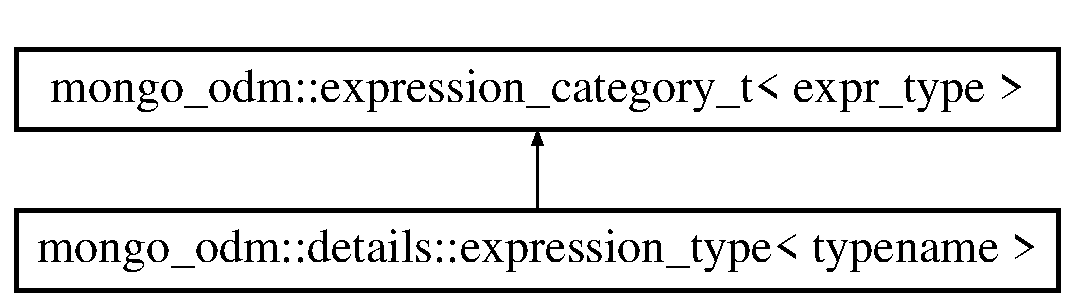
\includegraphics[height=2.000000cm]{structmongo__odm_1_1details_1_1expression__type}
\end{center}
\end{figure}


The documentation for this struct was generated from the following file\+:\begin{DoxyCompactItemize}
\item 
src/mongo\+\_\+odm/expression\+\_\+syntax.\+hpp\end{DoxyCompactItemize}

\hypertarget{structmongo__odm_1_1details_1_1expression__type_3_01add__to__set__update__expr_3_01NvpT_00_01U_01_4_01_4}{}\section{mongo\+\_\+odm\+:\+:details\+:\+:expression\+\_\+type$<$ add\+\_\+to\+\_\+set\+\_\+update\+\_\+expr$<$ NvpT, U $>$ $>$ Struct Template Reference}
\label{structmongo__odm_1_1details_1_1expression__type_3_01add__to__set__update__expr_3_01NvpT_00_01U_01_4_01_4}\index{mongo\+\_\+odm\+::details\+::expression\+\_\+type$<$ add\+\_\+to\+\_\+set\+\_\+update\+\_\+expr$<$ Nvp\+T, U $>$ $>$@{mongo\+\_\+odm\+::details\+::expression\+\_\+type$<$ add\+\_\+to\+\_\+set\+\_\+update\+\_\+expr$<$ Nvp\+T, U $>$ $>$}}
Inheritance diagram for mongo\+\_\+odm\+:\+:details\+:\+:expression\+\_\+type$<$ add\+\_\+to\+\_\+set\+\_\+update\+\_\+expr$<$ NvpT, U $>$ $>$\+:\begin{figure}[H]
\begin{center}
\leavevmode
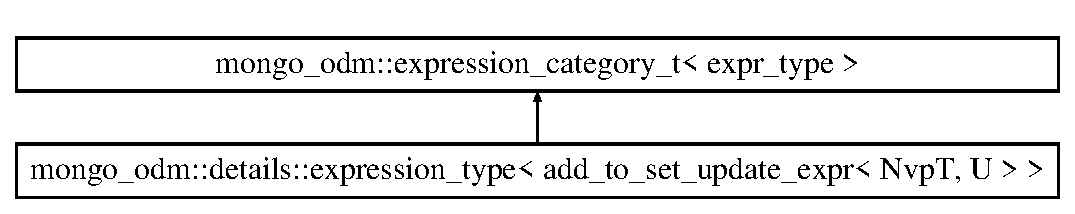
\includegraphics[height=2.000000cm]{structmongo__odm_1_1details_1_1expression__type_3_01add__to__set__update__expr_3_01NvpT_00_01U_01_4_01_4}
\end{center}
\end{figure}


The documentation for this struct was generated from the following file\+:\begin{DoxyCompactItemize}
\item 
src/mongo\+\_\+odm/expression\+\_\+syntax.\+hpp\end{DoxyCompactItemize}

\hypertarget{structmongo__odm_1_1details_1_1expression__type_3_01bit__update__expr_3_01NvpT_00_01Integer_01_4_01_4}{}\section{mongo\+\_\+odm\+:\+:details\+:\+:expression\+\_\+type$<$ bit\+\_\+update\+\_\+expr$<$ NvpT, Integer $>$ $>$ Struct Template Reference}
\label{structmongo__odm_1_1details_1_1expression__type_3_01bit__update__expr_3_01NvpT_00_01Integer_01_4_01_4}\index{mongo\+\_\+odm\+::details\+::expression\+\_\+type$<$ bit\+\_\+update\+\_\+expr$<$ Nvp\+T, Integer $>$ $>$@{mongo\+\_\+odm\+::details\+::expression\+\_\+type$<$ bit\+\_\+update\+\_\+expr$<$ Nvp\+T, Integer $>$ $>$}}
Inheritance diagram for mongo\+\_\+odm\+:\+:details\+:\+:expression\+\_\+type$<$ bit\+\_\+update\+\_\+expr$<$ NvpT, Integer $>$ $>$\+:\begin{figure}[H]
\begin{center}
\leavevmode
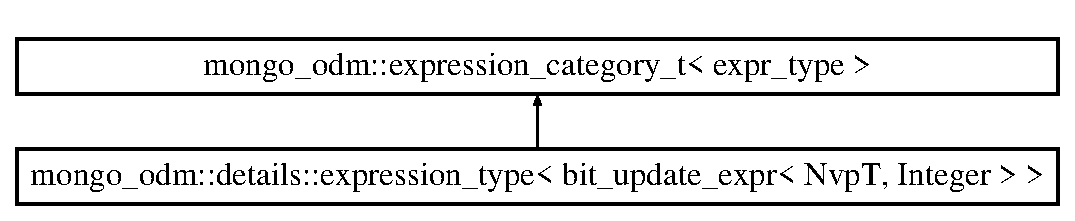
\includegraphics[height=2.000000cm]{structmongo__odm_1_1details_1_1expression__type_3_01bit__update__expr_3_01NvpT_00_01Integer_01_4_01_4}
\end{center}
\end{figure}


The documentation for this struct was generated from the following file\+:\begin{DoxyCompactItemize}
\item 
src/mongo\+\_\+odm/expression\+\_\+syntax.\+hpp\end{DoxyCompactItemize}

\hypertarget{structmongo__odm_1_1details_1_1expression__type_3_01boolean__expr_3_01Expr1_00_01Expr2_01_4_01_4}{}\section{mongo\+\_\+odm\+:\+:details\+:\+:expression\+\_\+type$<$ boolean\+\_\+expr$<$ Expr1, Expr2 $>$ $>$ Struct Template Reference}
\label{structmongo__odm_1_1details_1_1expression__type_3_01boolean__expr_3_01Expr1_00_01Expr2_01_4_01_4}\index{mongo\+\_\+odm\+::details\+::expression\+\_\+type$<$ boolean\+\_\+expr$<$ Expr1, Expr2 $>$ $>$@{mongo\+\_\+odm\+::details\+::expression\+\_\+type$<$ boolean\+\_\+expr$<$ Expr1, Expr2 $>$ $>$}}
Inheritance diagram for mongo\+\_\+odm\+:\+:details\+:\+:expression\+\_\+type$<$ boolean\+\_\+expr$<$ Expr1, Expr2 $>$ $>$\+:\begin{figure}[H]
\begin{center}
\leavevmode
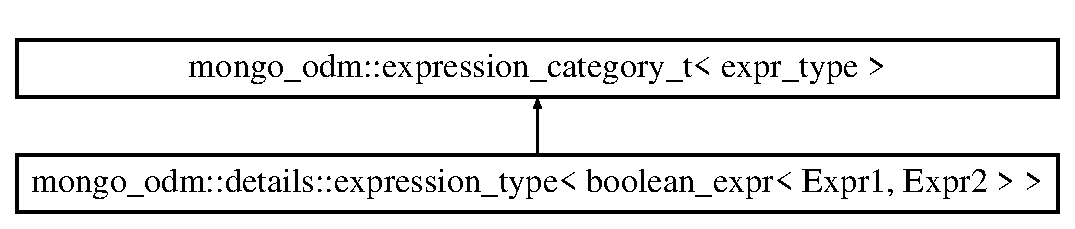
\includegraphics[height=2.000000cm]{structmongo__odm_1_1details_1_1expression__type_3_01boolean__expr_3_01Expr1_00_01Expr2_01_4_01_4}
\end{center}
\end{figure}


The documentation for this struct was generated from the following file\+:\begin{DoxyCompactItemize}
\item 
src/mongo\+\_\+odm/expression\+\_\+syntax.\+hpp\end{DoxyCompactItemize}

\hypertarget{structmongo__odm_1_1details_1_1expression__type_3_01boolean__list__expr_3_01List_01_4_01_4}{}\section{mongo\+\_\+odm\+:\+:details\+:\+:expression\+\_\+type$<$ boolean\+\_\+list\+\_\+expr$<$ List $>$ $>$ Struct Template Reference}
\label{structmongo__odm_1_1details_1_1expression__type_3_01boolean__list__expr_3_01List_01_4_01_4}\index{mongo\+\_\+odm\+::details\+::expression\+\_\+type$<$ boolean\+\_\+list\+\_\+expr$<$ List $>$ $>$@{mongo\+\_\+odm\+::details\+::expression\+\_\+type$<$ boolean\+\_\+list\+\_\+expr$<$ List $>$ $>$}}
Inheritance diagram for mongo\+\_\+odm\+:\+:details\+:\+:expression\+\_\+type$<$ boolean\+\_\+list\+\_\+expr$<$ List $>$ $>$\+:\begin{figure}[H]
\begin{center}
\leavevmode
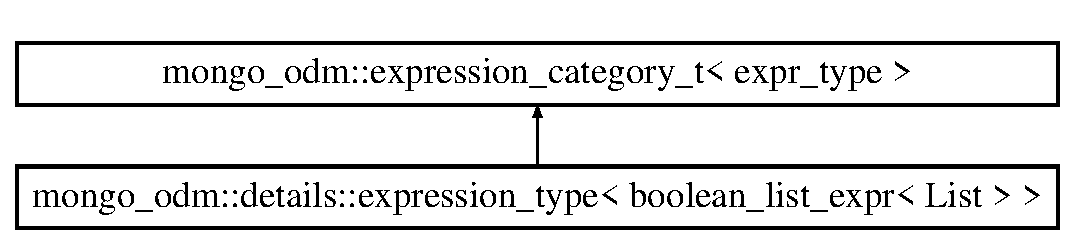
\includegraphics[height=2.000000cm]{structmongo__odm_1_1details_1_1expression__type_3_01boolean__list__expr_3_01List_01_4_01_4}
\end{center}
\end{figure}


The documentation for this struct was generated from the following file\+:\begin{DoxyCompactItemize}
\item 
src/mongo\+\_\+odm/expression\+\_\+syntax.\+hpp\end{DoxyCompactItemize}

\hypertarget{structmongo__odm_1_1details_1_1expression__type_3_01comparison__expr_3_01NvpT_00_01U_01_4_01_4}{}\section{mongo\+\_\+odm\+:\+:details\+:\+:expression\+\_\+type$<$ comparison\+\_\+expr$<$ NvpT, U $>$ $>$ Struct Template Reference}
\label{structmongo__odm_1_1details_1_1expression__type_3_01comparison__expr_3_01NvpT_00_01U_01_4_01_4}\index{mongo\+\_\+odm\+::details\+::expression\+\_\+type$<$ comparison\+\_\+expr$<$ Nvp\+T, U $>$ $>$@{mongo\+\_\+odm\+::details\+::expression\+\_\+type$<$ comparison\+\_\+expr$<$ Nvp\+T, U $>$ $>$}}
Inheritance diagram for mongo\+\_\+odm\+:\+:details\+:\+:expression\+\_\+type$<$ comparison\+\_\+expr$<$ NvpT, U $>$ $>$\+:\begin{figure}[H]
\begin{center}
\leavevmode
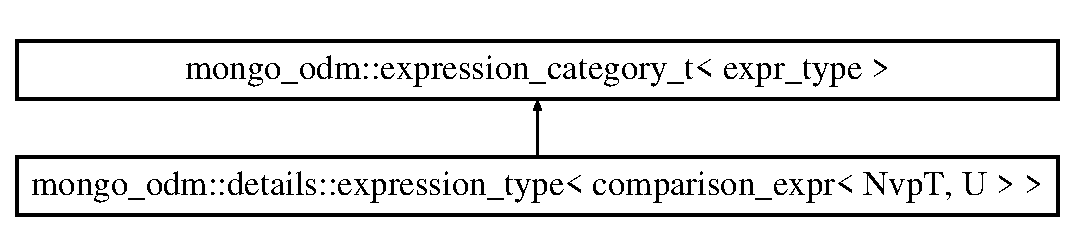
\includegraphics[height=2.000000cm]{structmongo__odm_1_1details_1_1expression__type_3_01comparison__expr_3_01NvpT_00_01U_01_4_01_4}
\end{center}
\end{figure}


The documentation for this struct was generated from the following file\+:\begin{DoxyCompactItemize}
\item 
src/mongo\+\_\+odm/expression\+\_\+syntax.\+hpp\end{DoxyCompactItemize}

\hypertarget{structmongo__odm_1_1details_1_1expression__type_3_01comparison__value__expr_3_01NvpT_00_01U_01_4_01_4}{}\section{mongo\+\_\+odm\+:\+:details\+:\+:expression\+\_\+type$<$ comparison\+\_\+value\+\_\+expr$<$ NvpT, U $>$ $>$ Struct Template Reference}
\label{structmongo__odm_1_1details_1_1expression__type_3_01comparison__value__expr_3_01NvpT_00_01U_01_4_01_4}\index{mongo\+\_\+odm\+::details\+::expression\+\_\+type$<$ comparison\+\_\+value\+\_\+expr$<$ Nvp\+T, U $>$ $>$@{mongo\+\_\+odm\+::details\+::expression\+\_\+type$<$ comparison\+\_\+value\+\_\+expr$<$ Nvp\+T, U $>$ $>$}}
Inheritance diagram for mongo\+\_\+odm\+:\+:details\+:\+:expression\+\_\+type$<$ comparison\+\_\+value\+\_\+expr$<$ NvpT, U $>$ $>$\+:\begin{figure}[H]
\begin{center}
\leavevmode
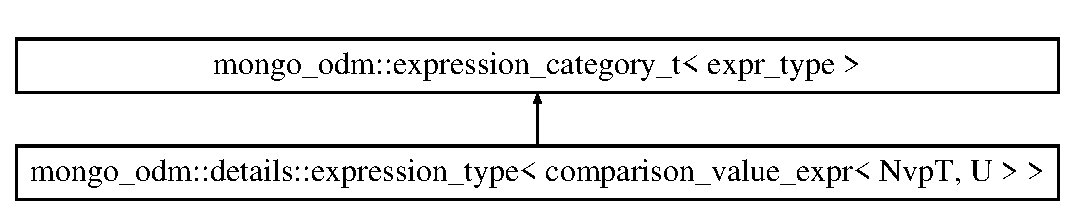
\includegraphics[height=2.000000cm]{structmongo__odm_1_1details_1_1expression__type_3_01comparison__value__expr_3_01NvpT_00_01U_01_4_01_4}
\end{center}
\end{figure}


The documentation for this struct was generated from the following file\+:\begin{DoxyCompactItemize}
\item 
src/mongo\+\_\+odm/expression\+\_\+syntax.\+hpp\end{DoxyCompactItemize}

\hypertarget{structmongo__odm_1_1details_1_1expression__type_3_01current__date__expr_3_01NvpT_01_4_01_4}{}\section{mongo\+\_\+odm\+:\+:details\+:\+:expression\+\_\+type$<$ current\+\_\+date\+\_\+expr$<$ NvpT $>$ $>$ Struct Template Reference}
\label{structmongo__odm_1_1details_1_1expression__type_3_01current__date__expr_3_01NvpT_01_4_01_4}\index{mongo\+\_\+odm\+::details\+::expression\+\_\+type$<$ current\+\_\+date\+\_\+expr$<$ Nvp\+T $>$ $>$@{mongo\+\_\+odm\+::details\+::expression\+\_\+type$<$ current\+\_\+date\+\_\+expr$<$ Nvp\+T $>$ $>$}}
Inheritance diagram for mongo\+\_\+odm\+:\+:details\+:\+:expression\+\_\+type$<$ current\+\_\+date\+\_\+expr$<$ NvpT $>$ $>$\+:\begin{figure}[H]
\begin{center}
\leavevmode
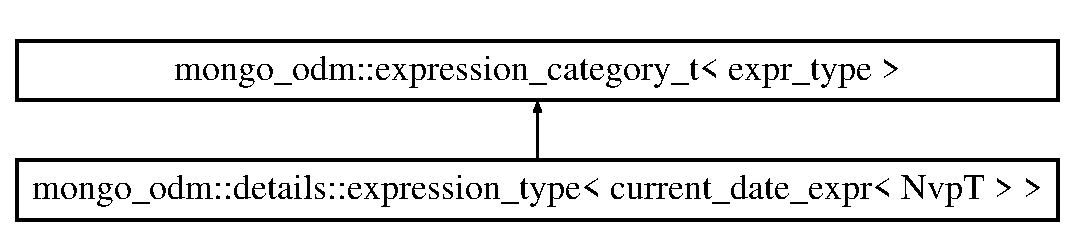
\includegraphics[height=2.000000cm]{structmongo__odm_1_1details_1_1expression__type_3_01current__date__expr_3_01NvpT_01_4_01_4}
\end{center}
\end{figure}


The documentation for this struct was generated from the following file\+:\begin{DoxyCompactItemize}
\item 
src/mongo\+\_\+odm/expression\+\_\+syntax.\+hpp\end{DoxyCompactItemize}

\hypertarget{structmongo__odm_1_1details_1_1expression__type_3_01expression__list_3_01list__type_00_01Args_8_8_8_01_4_01_4}{}\section{mongo\+\_\+odm\+:\+:details\+:\+:expression\+\_\+type$<$ expression\+\_\+list$<$ list\+\_\+type, Args... $>$ $>$ Struct Template Reference}
\label{structmongo__odm_1_1details_1_1expression__type_3_01expression__list_3_01list__type_00_01Args_8_8_8_01_4_01_4}\index{mongo\+\_\+odm\+::details\+::expression\+\_\+type$<$ expression\+\_\+list$<$ list\+\_\+type, Args... $>$ $>$@{mongo\+\_\+odm\+::details\+::expression\+\_\+type$<$ expression\+\_\+list$<$ list\+\_\+type, Args... $>$ $>$}}
Inheritance diagram for mongo\+\_\+odm\+:\+:details\+:\+:expression\+\_\+type$<$ expression\+\_\+list$<$ list\+\_\+type, Args... $>$ $>$\+:\begin{figure}[H]
\begin{center}
\leavevmode
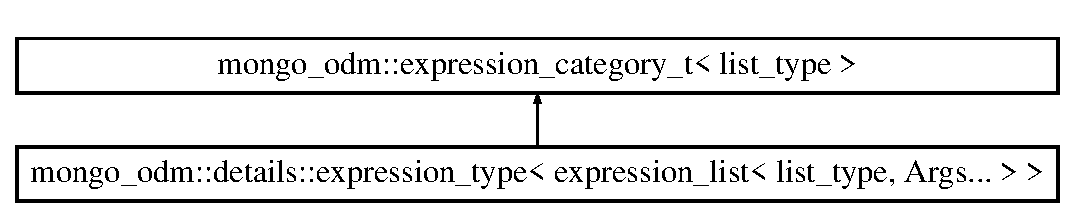
\includegraphics[height=2.000000cm]{structmongo__odm_1_1details_1_1expression__type_3_01expression__list_3_01list__type_00_01Args_8_8_8_01_4_01_4}
\end{center}
\end{figure}


The documentation for this struct was generated from the following file\+:\begin{DoxyCompactItemize}
\item 
src/mongo\+\_\+odm/expression\+\_\+syntax.\+hpp\end{DoxyCompactItemize}

\hypertarget{structmongo__odm_1_1details_1_1expression__type_3_01mod__expr_3_01NvpT_01_4_01_4}{}\section{mongo\+\_\+odm\+:\+:details\+:\+:expression\+\_\+type$<$ mod\+\_\+expr$<$ NvpT $>$ $>$ Struct Template Reference}
\label{structmongo__odm_1_1details_1_1expression__type_3_01mod__expr_3_01NvpT_01_4_01_4}\index{mongo\+\_\+odm\+::details\+::expression\+\_\+type$<$ mod\+\_\+expr$<$ Nvp\+T $>$ $>$@{mongo\+\_\+odm\+::details\+::expression\+\_\+type$<$ mod\+\_\+expr$<$ Nvp\+T $>$ $>$}}
Inheritance diagram for mongo\+\_\+odm\+:\+:details\+:\+:expression\+\_\+type$<$ mod\+\_\+expr$<$ NvpT $>$ $>$\+:\begin{figure}[H]
\begin{center}
\leavevmode
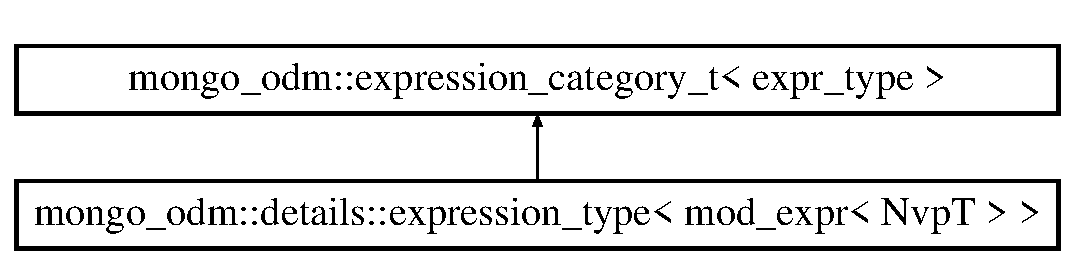
\includegraphics[height=2.000000cm]{structmongo__odm_1_1details_1_1expression__type_3_01mod__expr_3_01NvpT_01_4_01_4}
\end{center}
\end{figure}


The documentation for this struct was generated from the following file\+:\begin{DoxyCompactItemize}
\item 
src/mongo\+\_\+odm/expression\+\_\+syntax.\+hpp\end{DoxyCompactItemize}

\hypertarget{structmongo__odm_1_1details_1_1expression__type_3_01not__expr_3_01Expr_01_4_01_4}{}\section{mongo\+\_\+odm\+:\+:details\+:\+:expression\+\_\+type$<$ not\+\_\+expr$<$ Expr $>$ $>$ Struct Template Reference}
\label{structmongo__odm_1_1details_1_1expression__type_3_01not__expr_3_01Expr_01_4_01_4}\index{mongo\+\_\+odm\+::details\+::expression\+\_\+type$<$ not\+\_\+expr$<$ Expr $>$ $>$@{mongo\+\_\+odm\+::details\+::expression\+\_\+type$<$ not\+\_\+expr$<$ Expr $>$ $>$}}
Inheritance diagram for mongo\+\_\+odm\+:\+:details\+:\+:expression\+\_\+type$<$ not\+\_\+expr$<$ Expr $>$ $>$\+:\begin{figure}[H]
\begin{center}
\leavevmode
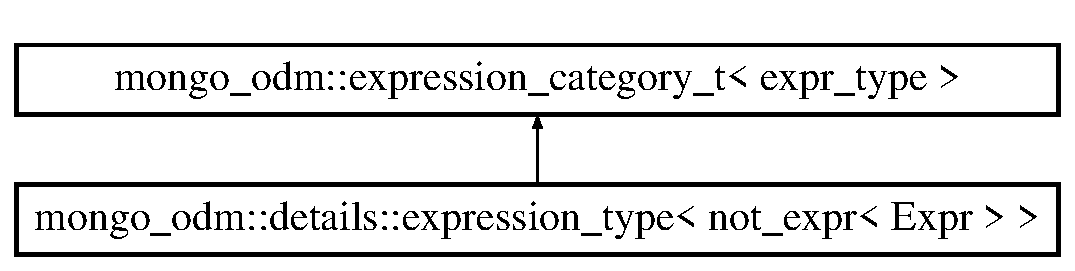
\includegraphics[height=2.000000cm]{structmongo__odm_1_1details_1_1expression__type_3_01not__expr_3_01Expr_01_4_01_4}
\end{center}
\end{figure}


The documentation for this struct was generated from the following file\+:\begin{DoxyCompactItemize}
\item 
src/mongo\+\_\+odm/expression\+\_\+syntax.\+hpp\end{DoxyCompactItemize}

\hypertarget{structmongo__odm_1_1details_1_1expression__type_3_01push__update__expr_3_01NvpT_00_01U_00_01Sort_01_4_01_4}{}\section{mongo\+\_\+odm\+:\+:details\+:\+:expression\+\_\+type$<$ push\+\_\+update\+\_\+expr$<$ NvpT, U, Sort $>$ $>$ Struct Template Reference}
\label{structmongo__odm_1_1details_1_1expression__type_3_01push__update__expr_3_01NvpT_00_01U_00_01Sort_01_4_01_4}\index{mongo\+\_\+odm\+::details\+::expression\+\_\+type$<$ push\+\_\+update\+\_\+expr$<$ Nvp\+T, U, Sort $>$ $>$@{mongo\+\_\+odm\+::details\+::expression\+\_\+type$<$ push\+\_\+update\+\_\+expr$<$ Nvp\+T, U, Sort $>$ $>$}}
Inheritance diagram for mongo\+\_\+odm\+:\+:details\+:\+:expression\+\_\+type$<$ push\+\_\+update\+\_\+expr$<$ NvpT, U, Sort $>$ $>$\+:\begin{figure}[H]
\begin{center}
\leavevmode
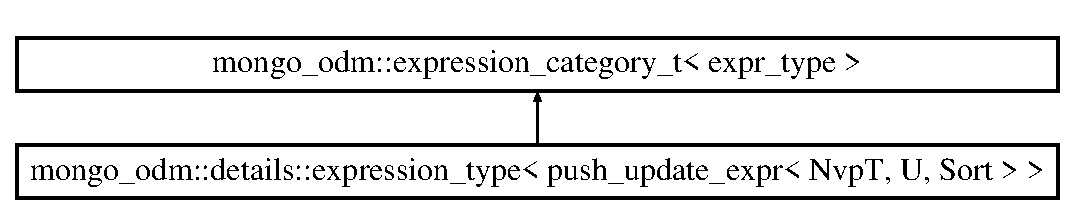
\includegraphics[height=2.000000cm]{structmongo__odm_1_1details_1_1expression__type_3_01push__update__expr_3_01NvpT_00_01U_00_01Sort_01_4_01_4}
\end{center}
\end{figure}


The documentation for this struct was generated from the following file\+:\begin{DoxyCompactItemize}
\item 
src/mongo\+\_\+odm/expression\+\_\+syntax.\+hpp\end{DoxyCompactItemize}

\hypertarget{structmongo__odm_1_1details_1_1expression__type_3_01sort__expr_3_01NvpT_01_4_01_4}{}\section{mongo\+\_\+odm\+:\+:details\+:\+:expression\+\_\+type$<$ sort\+\_\+expr$<$ NvpT $>$ $>$ Struct Template Reference}
\label{structmongo__odm_1_1details_1_1expression__type_3_01sort__expr_3_01NvpT_01_4_01_4}\index{mongo\+\_\+odm\+::details\+::expression\+\_\+type$<$ sort\+\_\+expr$<$ Nvp\+T $>$ $>$@{mongo\+\_\+odm\+::details\+::expression\+\_\+type$<$ sort\+\_\+expr$<$ Nvp\+T $>$ $>$}}
Inheritance diagram for mongo\+\_\+odm\+:\+:details\+:\+:expression\+\_\+type$<$ sort\+\_\+expr$<$ NvpT $>$ $>$\+:\begin{figure}[H]
\begin{center}
\leavevmode
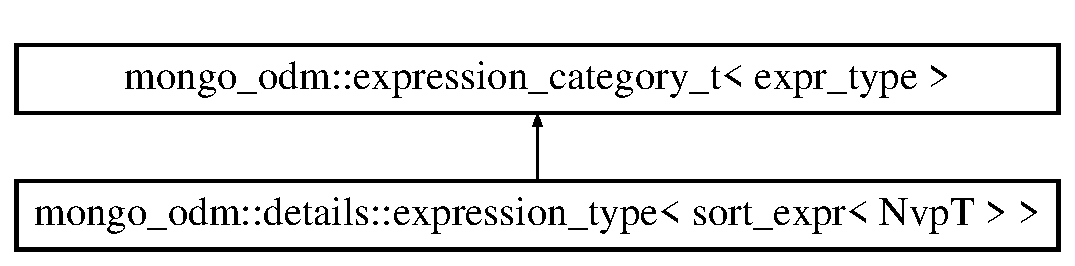
\includegraphics[height=2.000000cm]{structmongo__odm_1_1details_1_1expression__type_3_01sort__expr_3_01NvpT_01_4_01_4}
\end{center}
\end{figure}


The documentation for this struct was generated from the following file\+:\begin{DoxyCompactItemize}
\item 
src/mongo\+\_\+odm/expression\+\_\+syntax.\+hpp\end{DoxyCompactItemize}

\hypertarget{structmongo__odm_1_1details_1_1expression__type_3_01text__search__expr_01_4}{}\section{mongo\+\_\+odm\+:\+:details\+:\+:expression\+\_\+type$<$ text\+\_\+search\+\_\+expr $>$ Struct Template Reference}
\label{structmongo__odm_1_1details_1_1expression__type_3_01text__search__expr_01_4}\index{mongo\+\_\+odm\+::details\+::expression\+\_\+type$<$ text\+\_\+search\+\_\+expr $>$@{mongo\+\_\+odm\+::details\+::expression\+\_\+type$<$ text\+\_\+search\+\_\+expr $>$}}
Inheritance diagram for mongo\+\_\+odm\+:\+:details\+:\+:expression\+\_\+type$<$ text\+\_\+search\+\_\+expr $>$\+:\begin{figure}[H]
\begin{center}
\leavevmode
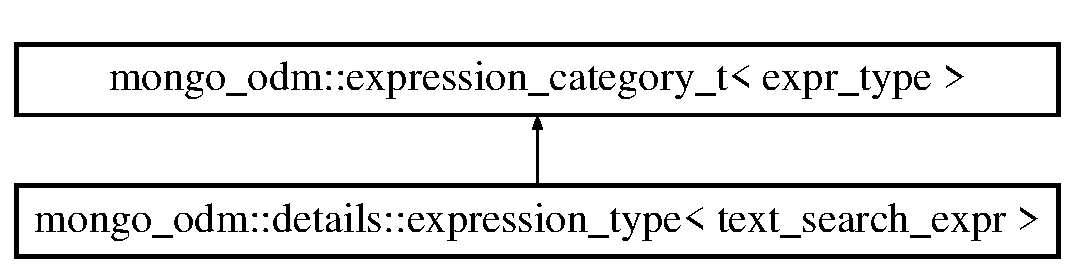
\includegraphics[height=2.000000cm]{structmongo__odm_1_1details_1_1expression__type_3_01text__search__expr_01_4}
\end{center}
\end{figure}


The documentation for this struct was generated from the following file\+:\begin{DoxyCompactItemize}
\item 
src/mongo\+\_\+odm/expression\+\_\+syntax.\+hpp\end{DoxyCompactItemize}

\hypertarget{structmongo__odm_1_1details_1_1expression__type_3_01unset__expr_3_01NvpT_01_4_01_4}{}\section{mongo\+\_\+odm\+:\+:details\+:\+:expression\+\_\+type$<$ unset\+\_\+expr$<$ NvpT $>$ $>$ Struct Template Reference}
\label{structmongo__odm_1_1details_1_1expression__type_3_01unset__expr_3_01NvpT_01_4_01_4}\index{mongo\+\_\+odm\+::details\+::expression\+\_\+type$<$ unset\+\_\+expr$<$ Nvp\+T $>$ $>$@{mongo\+\_\+odm\+::details\+::expression\+\_\+type$<$ unset\+\_\+expr$<$ Nvp\+T $>$ $>$}}
Inheritance diagram for mongo\+\_\+odm\+:\+:details\+:\+:expression\+\_\+type$<$ unset\+\_\+expr$<$ NvpT $>$ $>$\+:\begin{figure}[H]
\begin{center}
\leavevmode
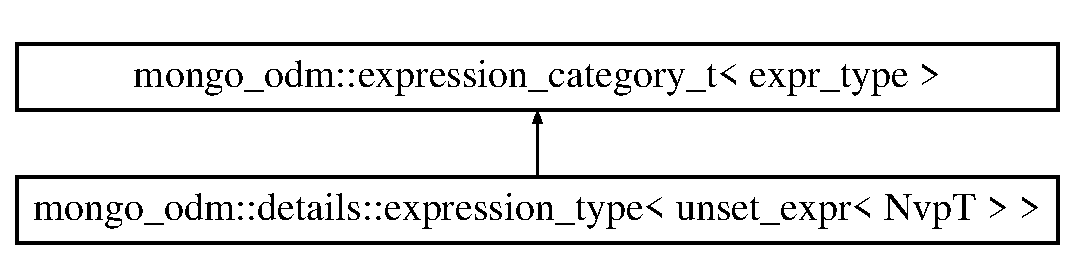
\includegraphics[height=2.000000cm]{structmongo__odm_1_1details_1_1expression__type_3_01unset__expr_3_01NvpT_01_4_01_4}
\end{center}
\end{figure}


The documentation for this struct was generated from the following file\+:\begin{DoxyCompactItemize}
\item 
src/mongo\+\_\+odm/expression\+\_\+syntax.\+hpp\end{DoxyCompactItemize}

\hypertarget{structmongo__odm_1_1details_1_1expression__type_3_01update__expr_3_01NvpT_00_01U_01_4_01_4}{}\section{mongo\+\_\+odm\+:\+:details\+:\+:expression\+\_\+type$<$ update\+\_\+expr$<$ NvpT, U $>$ $>$ Struct Template Reference}
\label{structmongo__odm_1_1details_1_1expression__type_3_01update__expr_3_01NvpT_00_01U_01_4_01_4}\index{mongo\+\_\+odm\+::details\+::expression\+\_\+type$<$ update\+\_\+expr$<$ Nvp\+T, U $>$ $>$@{mongo\+\_\+odm\+::details\+::expression\+\_\+type$<$ update\+\_\+expr$<$ Nvp\+T, U $>$ $>$}}
Inheritance diagram for mongo\+\_\+odm\+:\+:details\+:\+:expression\+\_\+type$<$ update\+\_\+expr$<$ NvpT, U $>$ $>$\+:\begin{figure}[H]
\begin{center}
\leavevmode
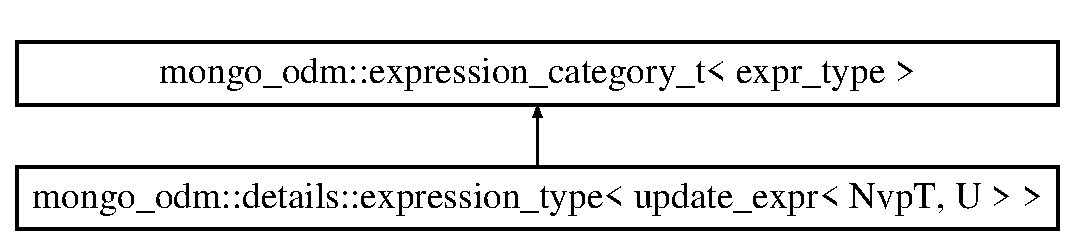
\includegraphics[height=2.000000cm]{structmongo__odm_1_1details_1_1expression__type_3_01update__expr_3_01NvpT_00_01U_01_4_01_4}
\end{center}
\end{figure}


The documentation for this struct was generated from the following file\+:\begin{DoxyCompactItemize}
\item 
src/mongo\+\_\+odm/expression\+\_\+syntax.\+hpp\end{DoxyCompactItemize}

\hypertarget{structmongo__odm_1_1details_1_1expression__type_3_01update__value__expr_3_01NvpT_00_01U_01_4_01_4}{}\section{mongo\+\_\+odm\+:\+:details\+:\+:expression\+\_\+type$<$ update\+\_\+value\+\_\+expr$<$ NvpT, U $>$ $>$ Struct Template Reference}
\label{structmongo__odm_1_1details_1_1expression__type_3_01update__value__expr_3_01NvpT_00_01U_01_4_01_4}\index{mongo\+\_\+odm\+::details\+::expression\+\_\+type$<$ update\+\_\+value\+\_\+expr$<$ Nvp\+T, U $>$ $>$@{mongo\+\_\+odm\+::details\+::expression\+\_\+type$<$ update\+\_\+value\+\_\+expr$<$ Nvp\+T, U $>$ $>$}}
Inheritance diagram for mongo\+\_\+odm\+:\+:details\+:\+:expression\+\_\+type$<$ update\+\_\+value\+\_\+expr$<$ NvpT, U $>$ $>$\+:\begin{figure}[H]
\begin{center}
\leavevmode
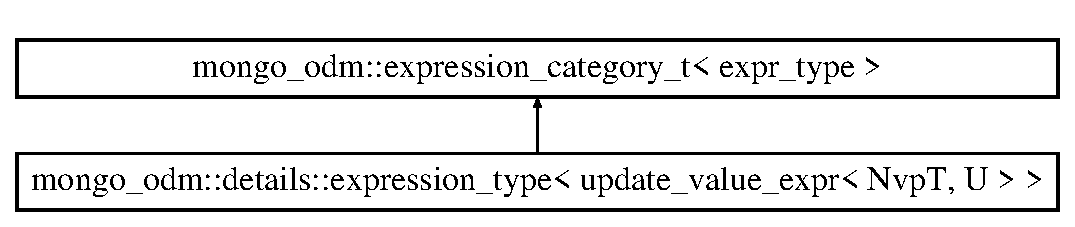
\includegraphics[height=2.000000cm]{structmongo__odm_1_1details_1_1expression__type_3_01update__value__expr_3_01NvpT_00_01U_01_4_01_4}
\end{center}
\end{figure}


The documentation for this struct was generated from the following file\+:\begin{DoxyCompactItemize}
\item 
src/mongo\+\_\+odm/expression\+\_\+syntax.\+hpp\end{DoxyCompactItemize}

\hypertarget{structmongo__odm_1_1FirstTypeIsTheSame}{}\section{mongo\+\_\+odm\+:\+:First\+Type\+Is\+The\+Same$<$ Ts $>$ Struct Template Reference}
\label{structmongo__odm_1_1FirstTypeIsTheSame}\index{mongo\+\_\+odm\+::\+First\+Type\+Is\+The\+Same$<$ Ts $>$@{mongo\+\_\+odm\+::\+First\+Type\+Is\+The\+Same$<$ Ts $>$}}


Helper type trait widget that helps properly forward arguments to \+\_\+id constructor.  




{\ttfamily \#include $<$model.\+hpp$>$}

Inheritance diagram for mongo\+\_\+odm\+:\+:First\+Type\+Is\+The\+Same$<$ Ts $>$\+:\begin{figure}[H]
\begin{center}
\leavevmode
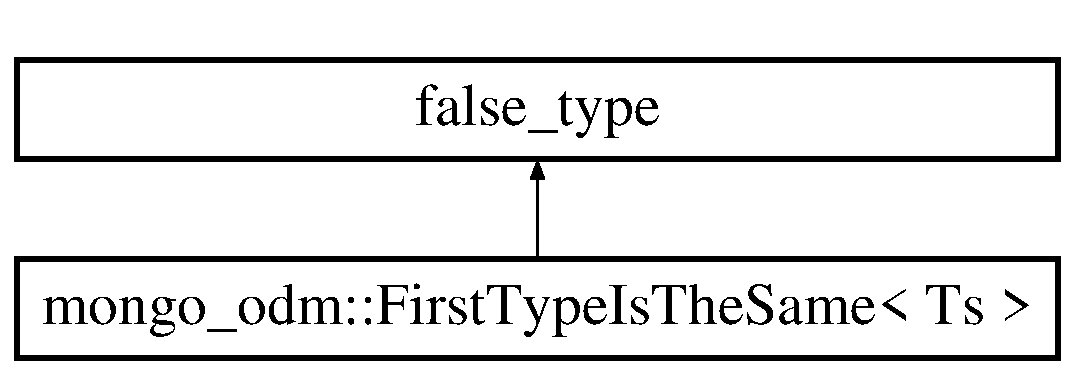
\includegraphics[height=2.000000cm]{structmongo__odm_1_1FirstTypeIsTheSame}
\end{center}
\end{figure}


\subsection{Detailed Description}
\subsubsection*{template$<$typename... Ts$>$\\*
struct mongo\+\_\+odm\+::\+First\+Type\+Is\+The\+Same$<$ Ts $>$}

Helper type trait widget that helps properly forward arguments to \+\_\+id constructor. 

First\+Type\+Is\+The\+Same$<$\+T1, T2, ...$>$\+::value will be true when T1 and T2 are of the same type, and false otherwise. 

The documentation for this struct was generated from the following file\+:\begin{DoxyCompactItemize}
\item 
src/mongo\+\_\+odm/model.\+hpp\end{DoxyCompactItemize}

\hypertarget{structmongo__odm_1_1FirstTypeIsTheSame_3_01T_00_01T2_00_01Ts_8_8_8_01_4}{}\section{mongo\+\_\+odm\+:\+:First\+Type\+Is\+The\+Same$<$ T, T2, Ts... $>$ Struct Template Reference}
\label{structmongo__odm_1_1FirstTypeIsTheSame_3_01T_00_01T2_00_01Ts_8_8_8_01_4}\index{mongo\+\_\+odm\+::\+First\+Type\+Is\+The\+Same$<$ T, T2, Ts... $>$@{mongo\+\_\+odm\+::\+First\+Type\+Is\+The\+Same$<$ T, T2, Ts... $>$}}
Inheritance diagram for mongo\+\_\+odm\+:\+:First\+Type\+Is\+The\+Same$<$ T, T2, Ts... $>$\+:\begin{figure}[H]
\begin{center}
\leavevmode
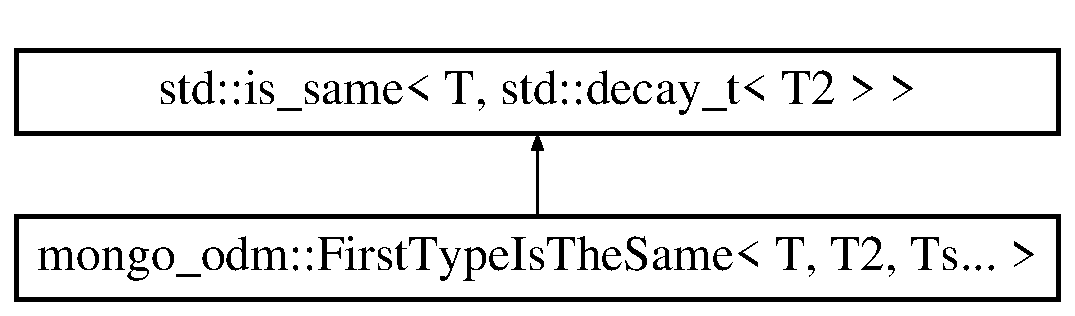
\includegraphics[height=2.000000cm]{structmongo__odm_1_1FirstTypeIsTheSame_3_01T_00_01T2_00_01Ts_8_8_8_01_4}
\end{center}
\end{figure}


The documentation for this struct was generated from the following file\+:\begin{DoxyCompactItemize}
\item 
src/mongo\+\_\+odm/model.\+hpp\end{DoxyCompactItemize}

\hypertarget{classmongo__odm_1_1free__nvp}{}\section{mongo\+\_\+odm\+:\+:free\+\_\+nvp$<$ T $>$ Class Template Reference}
\label{classmongo__odm_1_1free__nvp}\index{mongo\+\_\+odm\+::free\+\_\+nvp$<$ T $>$@{mongo\+\_\+odm\+::free\+\_\+nvp$<$ T $>$}}


Represents a field that does not have a name, i.\+e.  




{\ttfamily \#include $<$nvp.\+hpp$>$}

Inheritance diagram for mongo\+\_\+odm\+:\+:free\+\_\+nvp$<$ T $>$\+:\begin{figure}[H]
\begin{center}
\leavevmode
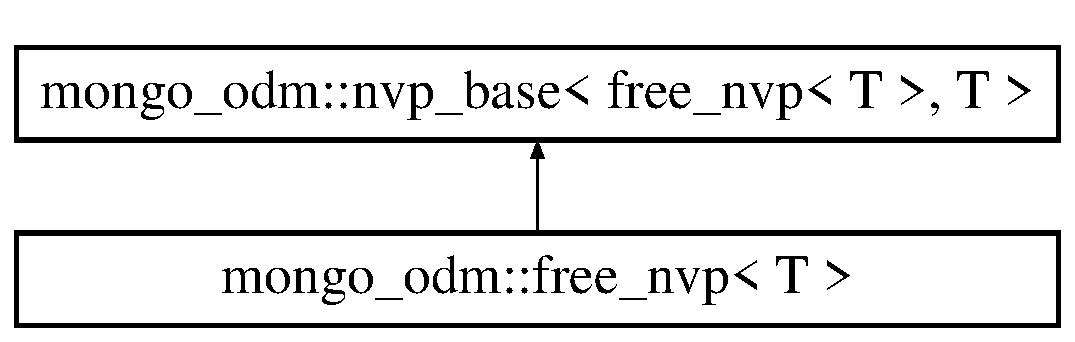
\includegraphics[height=2.000000cm]{classmongo__odm_1_1free__nvp}
\end{center}
\end{figure}
\subsection*{Additional Inherited Members}


\subsection{Detailed Description}
\subsubsection*{template$<$typename T$>$\\*
class mongo\+\_\+odm\+::free\+\_\+nvp$<$ T $>$}

Represents a field that does not have a name, i.\+e. 

an array element. This is used in \$elem\+Match expressions on scalar arrays, where the elements can be compared but don\textquotesingle{}t have fields of their own. 
\begin{DoxyTemplParams}{Template Parameters}
{\em T} & The type of the field. \\
\hline
\end{DoxyTemplParams}


The documentation for this class was generated from the following file\+:\begin{DoxyCompactItemize}
\item 
src/mongo\+\_\+odm/nvp.\+hpp\end{DoxyCompactItemize}

\hypertarget{structmongo__odm_1_1hasField}{}\section{mongo\+\_\+odm\+:\+:has\+Field$<$ Base, T, N, M, bool $>$ Struct Template Reference}
\label{structmongo__odm_1_1hasField}\index{mongo\+\_\+odm\+::has\+Field$<$ Base, T, N, M, bool $>$@{mongo\+\_\+odm\+::has\+Field$<$ Base, T, N, M, bool $>$}}


\hyperlink{structmongo__odm_1_1hasField}{has\+Field} determines whether a type Base has a member of the given type T as the Nth member out of M total members which have name value pairs.  




{\ttfamily \#include $<$nvp.\+hpp$>$}

Inheritance diagram for mongo\+\_\+odm\+:\+:has\+Field$<$ Base, T, N, M, bool $>$\+:\begin{figure}[H]
\begin{center}
\leavevmode
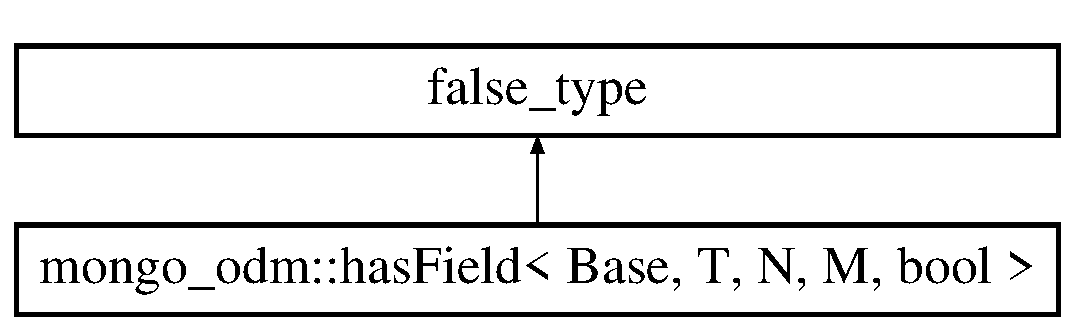
\includegraphics[height=2.000000cm]{structmongo__odm_1_1hasField}
\end{center}
\end{figure}


\subsection{Detailed Description}
\subsubsection*{template$<$typename Base, typename T, size\+\_\+t N, size\+\_\+t M, bool = (\+N $<$ M)$>$\\*
struct mongo\+\_\+odm\+::has\+Field$<$ Base, T, N, M, bool $>$}

\hyperlink{structmongo__odm_1_1hasField}{has\+Field} determines whether a type Base has a member of the given type T as the Nth member out of M total members which have name value pairs. 

The documentation for this struct was generated from the following file\+:\begin{DoxyCompactItemize}
\item 
src/mongo\+\_\+odm/nvp.\+hpp\end{DoxyCompactItemize}

\hypertarget{structmongo__odm_1_1hasField_3_01Base_00_01T_00_01N_00_01M_00_01true_01_4}{}\section{mongo\+\_\+odm\+:\+:has\+Field$<$ Base, T, N, M, true $>$ Struct Template Reference}
\label{structmongo__odm_1_1hasField_3_01Base_00_01T_00_01N_00_01M_00_01true_01_4}\index{mongo\+\_\+odm\+::has\+Field$<$ Base, T, N, M, true $>$@{mongo\+\_\+odm\+::has\+Field$<$ Base, T, N, M, true $>$}}
Inheritance diagram for mongo\+\_\+odm\+:\+:has\+Field$<$ Base, T, N, M, true $>$\+:\begin{figure}[H]
\begin{center}
\leavevmode
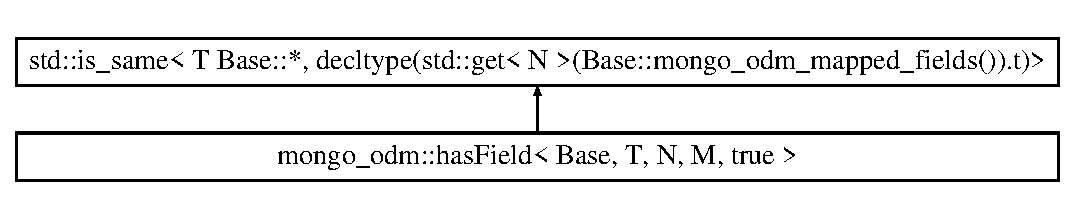
\includegraphics[height=2.000000cm]{structmongo__odm_1_1hasField_3_01Base_00_01T_00_01N_00_01M_00_01true_01_4}
\end{center}
\end{figure}


The documentation for this struct was generated from the following file\+:\begin{DoxyCompactItemize}
\item 
src/mongo\+\_\+odm/nvp.\+hpp\end{DoxyCompactItemize}

\hypertarget{structbson__mapper_1_1is__bson}{}\section{bson\+\_\+mapper\+:\+:is\+\_\+bson$<$ BsonT $>$ Struct Template Reference}
\label{structbson__mapper_1_1is__bson}\index{bson\+\_\+mapper\+::is\+\_\+bson$<$ Bson\+T $>$@{bson\+\_\+mapper\+::is\+\_\+bson$<$ Bson\+T $>$}}


A templated struct containing a bool value that specifies whether the provided template parameter is a B\+S\+ON type.  




{\ttfamily \#include $<$bson\+\_\+archiver.\+hpp$>$}



\subsection{Detailed Description}
\subsubsection*{template$<$class BsonT$>$\\*
struct bson\+\_\+mapper\+::is\+\_\+bson$<$ Bson\+T $>$}

A templated struct containing a bool value that specifies whether the provided template parameter is a B\+S\+ON type. 

The documentation for this struct was generated from the following file\+:\begin{DoxyCompactItemize}
\item 
src/bson\+\_\+mapper/bson\+\_\+archiver.\+hpp\end{DoxyCompactItemize}

\hypertarget{structbson__mapper_1_1is__bson__view}{}\section{bson\+\_\+mapper\+:\+:is\+\_\+bson\+\_\+view$<$ BsonT $>$ Struct Template Reference}
\label{structbson__mapper_1_1is__bson__view}\index{bson\+\_\+mapper\+::is\+\_\+bson\+\_\+view$<$ Bson\+T $>$@{bson\+\_\+mapper\+::is\+\_\+bson\+\_\+view$<$ Bson\+T $>$}}


A templated struct containing a bool value that specifies whether the provided template parameter is a B\+S\+ON type that contains a view.  




{\ttfamily \#include $<$bson\+\_\+archiver.\+hpp$>$}



\subsection{Detailed Description}
\subsubsection*{template$<$class BsonT$>$\\*
struct bson\+\_\+mapper\+::is\+\_\+bson\+\_\+view$<$ Bson\+T $>$}

A templated struct containing a bool value that specifies whether the provided template parameter is a B\+S\+ON type that contains a view. 

The documentation for this struct was generated from the following file\+:\begin{DoxyCompactItemize}
\item 
src/bson\+\_\+mapper/bson\+\_\+archiver.\+hpp\end{DoxyCompactItemize}

\hypertarget{structmongo__odm_1_1is__date}{}\section{mongo\+\_\+odm\+:\+:is\+\_\+date$<$ T $>$ Struct Template Reference}
\label{structmongo__odm_1_1is__date}\index{mongo\+\_\+odm\+::is\+\_\+date$<$ T $>$@{mongo\+\_\+odm\+::is\+\_\+date$<$ T $>$}}


A type traits struct that determines whether a certain type stores a date.  




{\ttfamily \#include $<$util.\+hpp$>$}

Inheritance diagram for mongo\+\_\+odm\+:\+:is\+\_\+date$<$ T $>$\+:\begin{figure}[H]
\begin{center}
\leavevmode
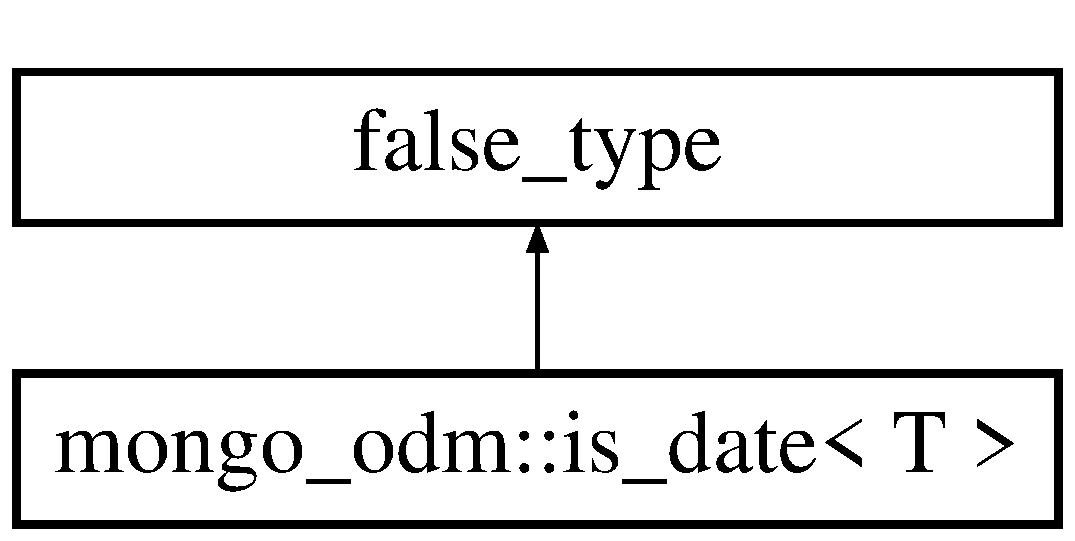
\includegraphics[height=2.000000cm]{structmongo__odm_1_1is__date}
\end{center}
\end{figure}


\subsection{Detailed Description}
\subsubsection*{template$<$typename T$>$\\*
struct mongo\+\_\+odm\+::is\+\_\+date$<$ T $>$}

A type traits struct that determines whether a certain type stores a date. 

This includes $<$chrono$>$ time types, and the B\+S\+ON b\+\_\+date type. time\+\_\+t is not included due to potential problems with conversion to B\+S\+ON. 

The documentation for this struct was generated from the following file\+:\begin{DoxyCompactItemize}
\item 
src/mongo\+\_\+odm/util.\+hpp\end{DoxyCompactItemize}

\hypertarget{structmongo__odm_1_1is__date_3_01bsoncxx_1_1types_1_1b__date_01_4}{}\section{mongo\+\_\+odm\+:\+:is\+\_\+date$<$ bsoncxx\+:\+:types\+:\+:b\+\_\+date $>$ Struct Template Reference}
\label{structmongo__odm_1_1is__date_3_01bsoncxx_1_1types_1_1b__date_01_4}\index{mongo\+\_\+odm\+::is\+\_\+date$<$ bsoncxx\+::types\+::b\+\_\+date $>$@{mongo\+\_\+odm\+::is\+\_\+date$<$ bsoncxx\+::types\+::b\+\_\+date $>$}}
Inheritance diagram for mongo\+\_\+odm\+:\+:is\+\_\+date$<$ bsoncxx\+:\+:types\+:\+:b\+\_\+date $>$\+:\begin{figure}[H]
\begin{center}
\leavevmode
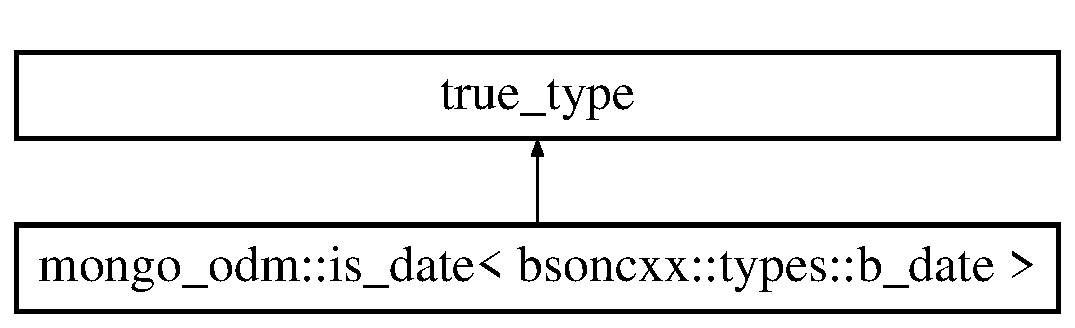
\includegraphics[height=2.000000cm]{structmongo__odm_1_1is__date_3_01bsoncxx_1_1types_1_1b__date_01_4}
\end{center}
\end{figure}


The documentation for this struct was generated from the following file\+:\begin{DoxyCompactItemize}
\item 
src/mongo\+\_\+odm/util.\+hpp\end{DoxyCompactItemize}

\hypertarget{structmongo__odm_1_1is__date_3_01std_1_1chrono_1_1duration_3_01Rep_00_01Period_01_4_01_4}{}\section{mongo\+\_\+odm\+:\+:is\+\_\+date$<$ std\+:\+:chrono\+:\+:duration$<$ Rep, Period $>$ $>$ Struct Template Reference}
\label{structmongo__odm_1_1is__date_3_01std_1_1chrono_1_1duration_3_01Rep_00_01Period_01_4_01_4}\index{mongo\+\_\+odm\+::is\+\_\+date$<$ std\+::chrono\+::duration$<$ Rep, Period $>$ $>$@{mongo\+\_\+odm\+::is\+\_\+date$<$ std\+::chrono\+::duration$<$ Rep, Period $>$ $>$}}
Inheritance diagram for mongo\+\_\+odm\+:\+:is\+\_\+date$<$ std\+:\+:chrono\+:\+:duration$<$ Rep, Period $>$ $>$\+:\begin{figure}[H]
\begin{center}
\leavevmode
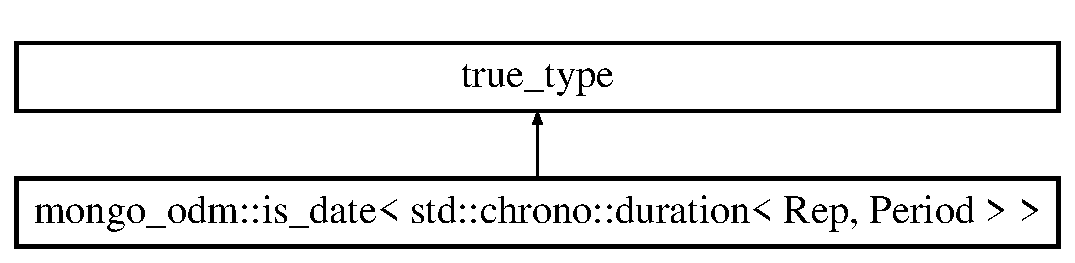
\includegraphics[height=2.000000cm]{structmongo__odm_1_1is__date_3_01std_1_1chrono_1_1duration_3_01Rep_00_01Period_01_4_01_4}
\end{center}
\end{figure}


The documentation for this struct was generated from the following file\+:\begin{DoxyCompactItemize}
\item 
src/mongo\+\_\+odm/util.\+hpp\end{DoxyCompactItemize}

\hypertarget{structmongo__odm_1_1is__date_3_01std_1_1chrono_1_1time__point_3_01Clock_00_01Duration_01_4_01_4}{}\section{mongo\+\_\+odm\+:\+:is\+\_\+date$<$ std\+:\+:chrono\+:\+:time\+\_\+point$<$ Clock, Duration $>$ $>$ Struct Template Reference}
\label{structmongo__odm_1_1is__date_3_01std_1_1chrono_1_1time__point_3_01Clock_00_01Duration_01_4_01_4}\index{mongo\+\_\+odm\+::is\+\_\+date$<$ std\+::chrono\+::time\+\_\+point$<$ Clock, Duration $>$ $>$@{mongo\+\_\+odm\+::is\+\_\+date$<$ std\+::chrono\+::time\+\_\+point$<$ Clock, Duration $>$ $>$}}
Inheritance diagram for mongo\+\_\+odm\+:\+:is\+\_\+date$<$ std\+:\+:chrono\+:\+:time\+\_\+point$<$ Clock, Duration $>$ $>$\+:\begin{figure}[H]
\begin{center}
\leavevmode
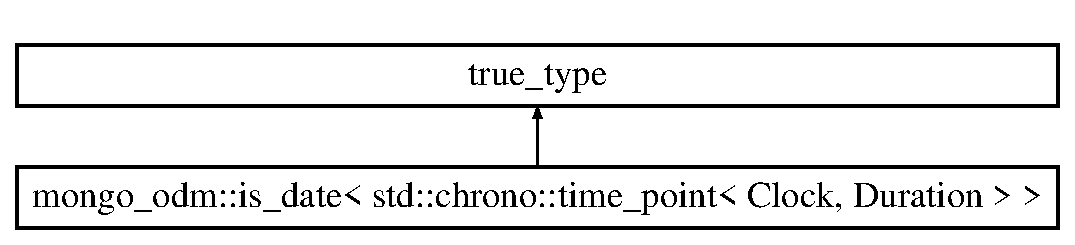
\includegraphics[height=2.000000cm]{structmongo__odm_1_1is__date_3_01std_1_1chrono_1_1time__point_3_01Clock_00_01Duration_01_4_01_4}
\end{center}
\end{figure}


The documentation for this struct was generated from the following file\+:\begin{DoxyCompactItemize}
\item 
src/mongo\+\_\+odm/util.\+hpp\end{DoxyCompactItemize}

\hypertarget{structmongo__odm_1_1details_1_1is__expression__type}{}\section{mongo\+\_\+odm\+:\+:details\+:\+:is\+\_\+expression\+\_\+type$<$ type, T $>$ Struct Template Reference}
\label{structmongo__odm_1_1details_1_1is__expression__type}\index{mongo\+\_\+odm\+::details\+::is\+\_\+expression\+\_\+type$<$ type, T $>$@{mongo\+\_\+odm\+::details\+::is\+\_\+expression\+\_\+type$<$ type, T $>$}}
Inheritance diagram for mongo\+\_\+odm\+:\+:details\+:\+:is\+\_\+expression\+\_\+type$<$ type, T $>$\+:\begin{figure}[H]
\begin{center}
\leavevmode
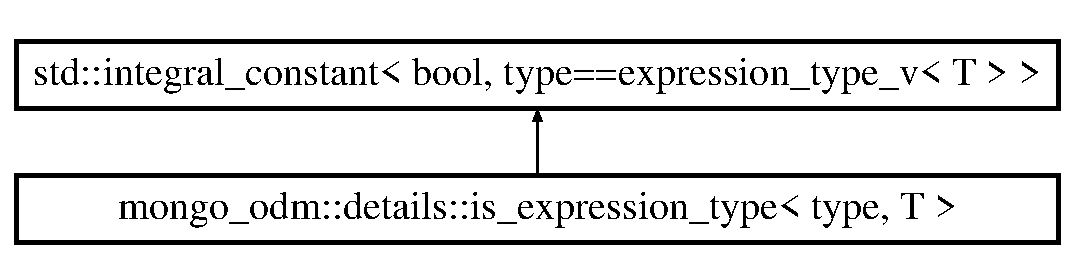
\includegraphics[height=2.000000cm]{structmongo__odm_1_1details_1_1is__expression__type}
\end{center}
\end{figure}


The documentation for this struct was generated from the following file\+:\begin{DoxyCompactItemize}
\item 
src/mongo\+\_\+odm/expression\+\_\+syntax.\+hpp\end{DoxyCompactItemize}

\hypertarget{structmongo__odm_1_1is__expression__type}{}\section{mongo\+\_\+odm\+:\+:is\+\_\+expression\+\_\+type$<$ expression\+\_\+category, typename $>$ Struct Template Reference}
\label{structmongo__odm_1_1is__expression__type}\index{mongo\+\_\+odm\+::is\+\_\+expression\+\_\+type$<$ expression\+\_\+category, typename $>$@{mongo\+\_\+odm\+::is\+\_\+expression\+\_\+type$<$ expression\+\_\+category, typename $>$}}


The documentation for this struct was generated from the following file\+:\begin{DoxyCompactItemize}
\item 
src/mongo\+\_\+odm/expression\+\_\+syntax.\+hpp\end{DoxyCompactItemize}

\hypertarget{structmongo__odm_1_1is__free__nvp}{}\section{mongo\+\_\+odm\+:\+:is\+\_\+free\+\_\+nvp$<$ NvpT $>$ Struct Template Reference}
\label{structmongo__odm_1_1is__free__nvp}\index{mongo\+\_\+odm\+::is\+\_\+free\+\_\+nvp$<$ Nvp\+T $>$@{mongo\+\_\+odm\+::is\+\_\+free\+\_\+nvp$<$ Nvp\+T $>$}}
Inheritance diagram for mongo\+\_\+odm\+:\+:is\+\_\+free\+\_\+nvp$<$ NvpT $>$\+:\begin{figure}[H]
\begin{center}
\leavevmode
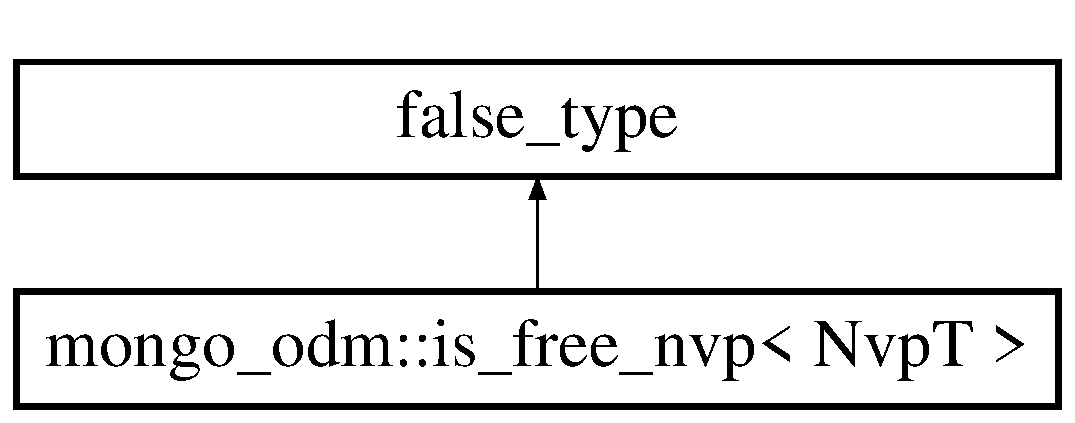
\includegraphics[height=2.000000cm]{structmongo__odm_1_1is__free__nvp}
\end{center}
\end{figure}


The documentation for this struct was generated from the following file\+:\begin{DoxyCompactItemize}
\item 
src/mongo\+\_\+odm/nvp.\+hpp\end{DoxyCompactItemize}

\hypertarget{structmongo__odm_1_1is__free__nvp_3_01free__nvp_3_01T_01_4_01_4}{}\section{mongo\+\_\+odm\+:\+:is\+\_\+free\+\_\+nvp$<$ free\+\_\+nvp$<$ T $>$ $>$ Struct Template Reference}
\label{structmongo__odm_1_1is__free__nvp_3_01free__nvp_3_01T_01_4_01_4}\index{mongo\+\_\+odm\+::is\+\_\+free\+\_\+nvp$<$ free\+\_\+nvp$<$ T $>$ $>$@{mongo\+\_\+odm\+::is\+\_\+free\+\_\+nvp$<$ free\+\_\+nvp$<$ T $>$ $>$}}
Inheritance diagram for mongo\+\_\+odm\+:\+:is\+\_\+free\+\_\+nvp$<$ free\+\_\+nvp$<$ T $>$ $>$\+:\begin{figure}[H]
\begin{center}
\leavevmode
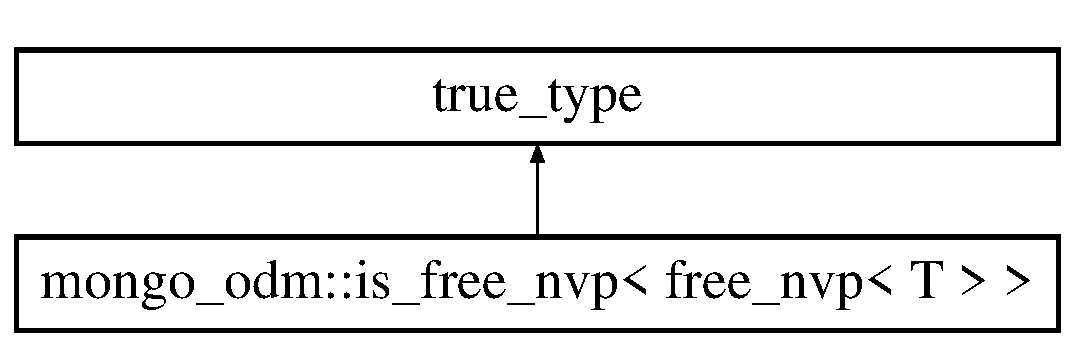
\includegraphics[height=2.000000cm]{structmongo__odm_1_1is__free__nvp_3_01free__nvp_3_01T_01_4_01_4}
\end{center}
\end{figure}


The documentation for this struct was generated from the following file\+:\begin{DoxyCompactItemize}
\item 
src/mongo\+\_\+odm/nvp.\+hpp\end{DoxyCompactItemize}

\hypertarget{structmongo__odm_1_1is__nvp}{}\section{mongo\+\_\+odm\+:\+:is\+\_\+nvp$<$ typename $>$ Struct Template Reference}
\label{structmongo__odm_1_1is__nvp}\index{mongo\+\_\+odm\+::is\+\_\+nvp$<$ typename $>$@{mongo\+\_\+odm\+::is\+\_\+nvp$<$ typename $>$}}


A type trait struct that inherits from std\+::true\+\_\+type if the given type parameter is a name-\/value pair, and from std\+::false\+\_\+type otherwise.  




{\ttfamily \#include $<$nvp.\+hpp$>$}

Inheritance diagram for mongo\+\_\+odm\+:\+:is\+\_\+nvp$<$ typename $>$\+:\begin{figure}[H]
\begin{center}
\leavevmode
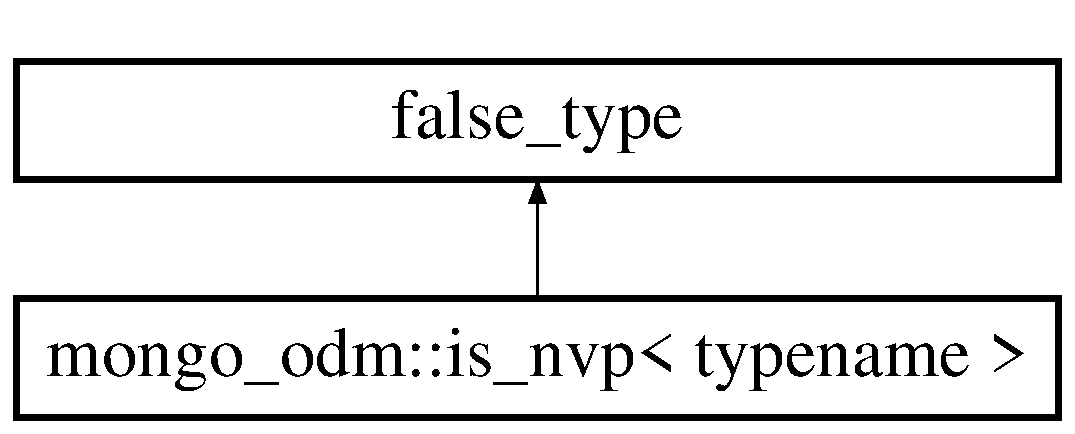
\includegraphics[height=2.000000cm]{structmongo__odm_1_1is__nvp}
\end{center}
\end{figure}


\subsection{Detailed Description}
\subsubsection*{template$<$typename$>$\\*
struct mongo\+\_\+odm\+::is\+\_\+nvp$<$ typename $>$}

A type trait struct that inherits from std\+::true\+\_\+type if the given type parameter is a name-\/value pair, and from std\+::false\+\_\+type otherwise. 

The documentation for this struct was generated from the following file\+:\begin{DoxyCompactItemize}
\item 
src/mongo\+\_\+odm/nvp.\+hpp\end{DoxyCompactItemize}

\hypertarget{structmongo__odm_1_1is__nvp_3_01array__element__nvp_3_01NvpT_01_4_01_4}{}\section{mongo\+\_\+odm\+:\+:is\+\_\+nvp$<$ array\+\_\+element\+\_\+nvp$<$ NvpT $>$ $>$ Struct Template Reference}
\label{structmongo__odm_1_1is__nvp_3_01array__element__nvp_3_01NvpT_01_4_01_4}\index{mongo\+\_\+odm\+::is\+\_\+nvp$<$ array\+\_\+element\+\_\+nvp$<$ Nvp\+T $>$ $>$@{mongo\+\_\+odm\+::is\+\_\+nvp$<$ array\+\_\+element\+\_\+nvp$<$ Nvp\+T $>$ $>$}}
Inheritance diagram for mongo\+\_\+odm\+:\+:is\+\_\+nvp$<$ array\+\_\+element\+\_\+nvp$<$ NvpT $>$ $>$\+:\begin{figure}[H]
\begin{center}
\leavevmode
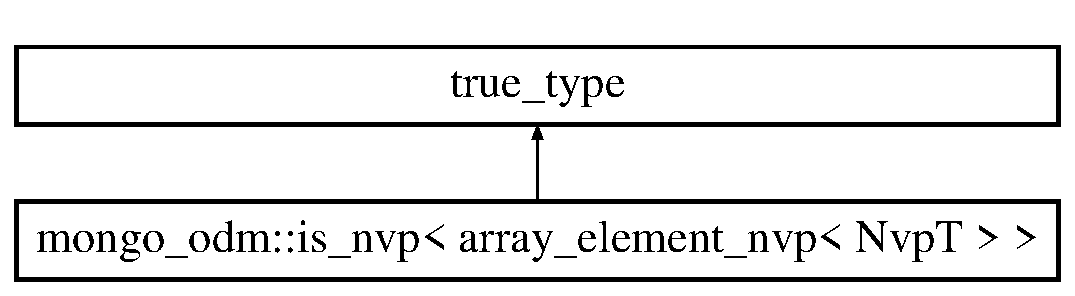
\includegraphics[height=2.000000cm]{structmongo__odm_1_1is__nvp_3_01array__element__nvp_3_01NvpT_01_4_01_4}
\end{center}
\end{figure}


The documentation for this struct was generated from the following file\+:\begin{DoxyCompactItemize}
\item 
src/mongo\+\_\+odm/nvp.\+hpp\end{DoxyCompactItemize}

\hypertarget{structmongo__odm_1_1is__nvp_3_01free__nvp_3_01T_01_4_01_4}{}\section{mongo\+\_\+odm\+:\+:is\+\_\+nvp$<$ free\+\_\+nvp$<$ T $>$ $>$ Struct Template Reference}
\label{structmongo__odm_1_1is__nvp_3_01free__nvp_3_01T_01_4_01_4}\index{mongo\+\_\+odm\+::is\+\_\+nvp$<$ free\+\_\+nvp$<$ T $>$ $>$@{mongo\+\_\+odm\+::is\+\_\+nvp$<$ free\+\_\+nvp$<$ T $>$ $>$}}
Inheritance diagram for mongo\+\_\+odm\+:\+:is\+\_\+nvp$<$ free\+\_\+nvp$<$ T $>$ $>$\+:\begin{figure}[H]
\begin{center}
\leavevmode
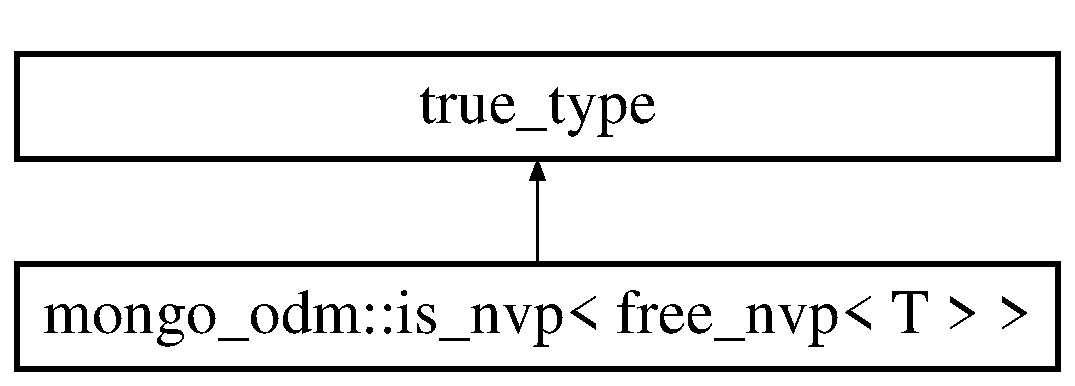
\includegraphics[height=2.000000cm]{structmongo__odm_1_1is__nvp_3_01free__nvp_3_01T_01_4_01_4}
\end{center}
\end{figure}


The documentation for this struct was generated from the following file\+:\begin{DoxyCompactItemize}
\item 
src/mongo\+\_\+odm/nvp.\+hpp\end{DoxyCompactItemize}

\hypertarget{structmongo__odm_1_1is__nvp_3_01nvp_3_01Base_00_01T_01_4_01_4}{}\section{mongo\+\_\+odm\+:\+:is\+\_\+nvp$<$ nvp$<$ Base, T $>$ $>$ Struct Template Reference}
\label{structmongo__odm_1_1is__nvp_3_01nvp_3_01Base_00_01T_01_4_01_4}\index{mongo\+\_\+odm\+::is\+\_\+nvp$<$ nvp$<$ Base, T $>$ $>$@{mongo\+\_\+odm\+::is\+\_\+nvp$<$ nvp$<$ Base, T $>$ $>$}}
Inheritance diagram for mongo\+\_\+odm\+:\+:is\+\_\+nvp$<$ nvp$<$ Base, T $>$ $>$\+:\begin{figure}[H]
\begin{center}
\leavevmode
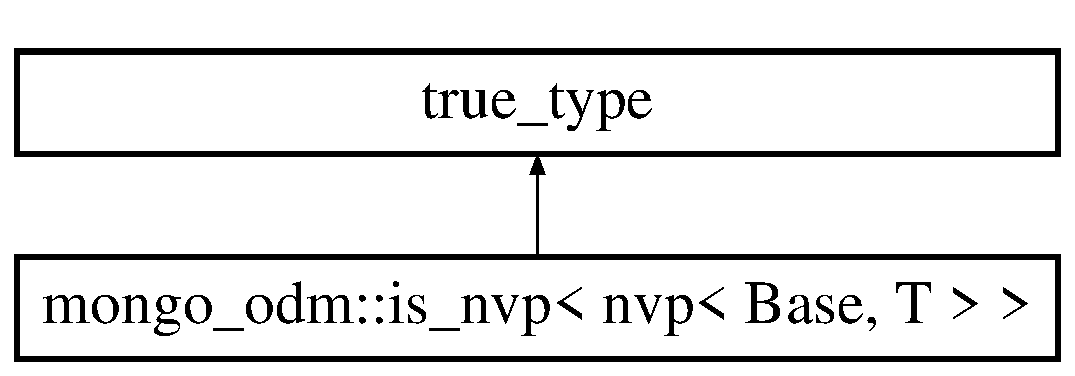
\includegraphics[height=2.000000cm]{structmongo__odm_1_1is__nvp_3_01nvp_3_01Base_00_01T_01_4_01_4}
\end{center}
\end{figure}


The documentation for this struct was generated from the following file\+:\begin{DoxyCompactItemize}
\item 
src/mongo\+\_\+odm/nvp.\+hpp\end{DoxyCompactItemize}

\hypertarget{structmongo__odm_1_1is__nvp_3_01nvp__child_3_01Base_00_01T_00_01Parent_01_4_01_4}{}\section{mongo\+\_\+odm\+:\+:is\+\_\+nvp$<$ nvp\+\_\+child$<$ Base, T, Parent $>$ $>$ Struct Template Reference}
\label{structmongo__odm_1_1is__nvp_3_01nvp__child_3_01Base_00_01T_00_01Parent_01_4_01_4}\index{mongo\+\_\+odm\+::is\+\_\+nvp$<$ nvp\+\_\+child$<$ Base, T, Parent $>$ $>$@{mongo\+\_\+odm\+::is\+\_\+nvp$<$ nvp\+\_\+child$<$ Base, T, Parent $>$ $>$}}
Inheritance diagram for mongo\+\_\+odm\+:\+:is\+\_\+nvp$<$ nvp\+\_\+child$<$ Base, T, Parent $>$ $>$\+:\begin{figure}[H]
\begin{center}
\leavevmode
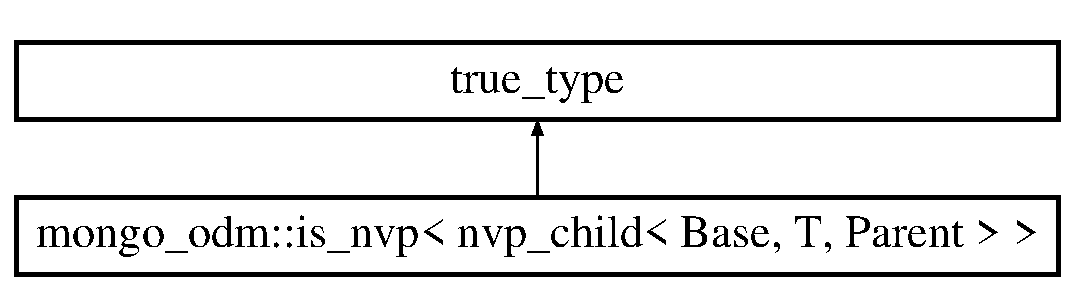
\includegraphics[height=2.000000cm]{structmongo__odm_1_1is__nvp_3_01nvp__child_3_01Base_00_01T_00_01Parent_01_4_01_4}
\end{center}
\end{figure}


The documentation for this struct was generated from the following file\+:\begin{DoxyCompactItemize}
\item 
src/mongo\+\_\+odm/nvp.\+hpp\end{DoxyCompactItemize}

\hypertarget{structmongo__odm_1_1is__optional}{}\section{mongo\+\_\+odm\+:\+:is\+\_\+optional$<$ T $>$ Struct Template Reference}
\label{structmongo__odm_1_1is__optional}\index{mongo\+\_\+odm\+::is\+\_\+optional$<$ T $>$@{mongo\+\_\+odm\+::is\+\_\+optional$<$ T $>$}}


A type trait struct for determining whether a type is an optional.  




{\ttfamily \#include $<$util.\+hpp$>$}

Inheritance diagram for mongo\+\_\+odm\+:\+:is\+\_\+optional$<$ T $>$\+:\begin{figure}[H]
\begin{center}
\leavevmode
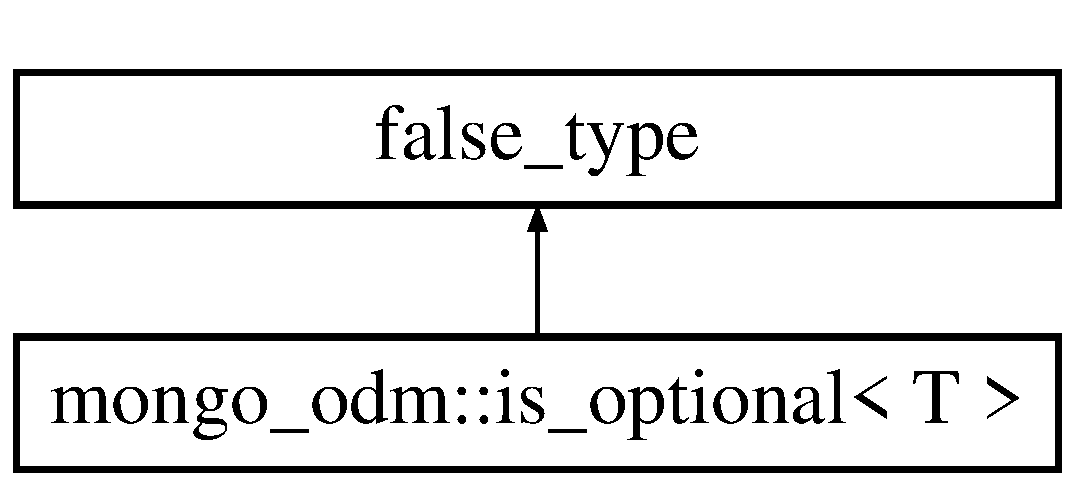
\includegraphics[height=2.000000cm]{structmongo__odm_1_1is__optional}
\end{center}
\end{figure}


\subsection{Detailed Description}
\subsubsection*{template$<$typename T$>$\\*
struct mongo\+\_\+odm\+::is\+\_\+optional$<$ T $>$}

A type trait struct for determining whether a type is an optional. 

The documentation for this struct was generated from the following file\+:\begin{DoxyCompactItemize}
\item 
src/mongo\+\_\+odm/util.\+hpp\end{DoxyCompactItemize}

\hypertarget{structmongo__odm_1_1is__optional_3_01bsoncxx_1_1stdx_1_1optional_3_01T_01_4_01_4}{}\section{mongo\+\_\+odm\+:\+:is\+\_\+optional$<$ bsoncxx\+:\+:stdx\+:\+:optional$<$ T $>$ $>$ Struct Template Reference}
\label{structmongo__odm_1_1is__optional_3_01bsoncxx_1_1stdx_1_1optional_3_01T_01_4_01_4}\index{mongo\+\_\+odm\+::is\+\_\+optional$<$ bsoncxx\+::stdx\+::optional$<$ T $>$ $>$@{mongo\+\_\+odm\+::is\+\_\+optional$<$ bsoncxx\+::stdx\+::optional$<$ T $>$ $>$}}
Inheritance diagram for mongo\+\_\+odm\+:\+:is\+\_\+optional$<$ bsoncxx\+:\+:stdx\+:\+:optional$<$ T $>$ $>$\+:\begin{figure}[H]
\begin{center}
\leavevmode
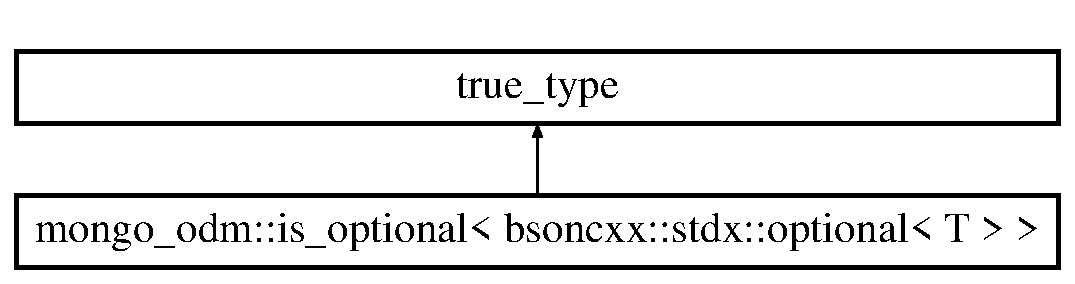
\includegraphics[height=2.000000cm]{structmongo__odm_1_1is__optional_3_01bsoncxx_1_1stdx_1_1optional_3_01T_01_4_01_4}
\end{center}
\end{figure}


The documentation for this struct was generated from the following file\+:\begin{DoxyCompactItemize}
\item 
src/mongo\+\_\+odm/util.\+hpp\end{DoxyCompactItemize}

\hypertarget{structmongo__odm_1_1details_1_1is__query__expression}{}\section{mongo\+\_\+odm\+:\+:details\+:\+:is\+\_\+query\+\_\+expression$<$ T $>$ Struct Template Reference}
\label{structmongo__odm_1_1details_1_1is__query__expression}\index{mongo\+\_\+odm\+::details\+::is\+\_\+query\+\_\+expression$<$ T $>$@{mongo\+\_\+odm\+::details\+::is\+\_\+query\+\_\+expression$<$ T $>$}}
Inheritance diagram for mongo\+\_\+odm\+:\+:details\+:\+:is\+\_\+query\+\_\+expression$<$ T $>$\+:\begin{figure}[H]
\begin{center}
\leavevmode
\includegraphics[height=3.000000cm]{structmongo__odm_1_1details_1_1is__query__expression}
\end{center}
\end{figure}


The documentation for this struct was generated from the following file\+:\begin{DoxyCompactItemize}
\item 
src/mongo\+\_\+odm/expression\+\_\+syntax.\+hpp\end{DoxyCompactItemize}

\hypertarget{structmongo__odm_1_1details_1_1is__sort__expression}{}\section{mongo\+\_\+odm\+:\+:details\+:\+:is\+\_\+sort\+\_\+expression$<$ T $>$ Struct Template Reference}
\label{structmongo__odm_1_1details_1_1is__sort__expression}\index{mongo\+\_\+odm\+::details\+::is\+\_\+sort\+\_\+expression$<$ T $>$@{mongo\+\_\+odm\+::details\+::is\+\_\+sort\+\_\+expression$<$ T $>$}}
Inheritance diagram for mongo\+\_\+odm\+:\+:details\+:\+:is\+\_\+sort\+\_\+expression$<$ T $>$\+:\begin{figure}[H]
\begin{center}
\leavevmode
\includegraphics[height=3.000000cm]{structmongo__odm_1_1details_1_1is__sort__expression}
\end{center}
\end{figure}


The documentation for this struct was generated from the following file\+:\begin{DoxyCompactItemize}
\item 
src/mongo\+\_\+odm/expression\+\_\+syntax.\+hpp\end{DoxyCompactItemize}

\hypertarget{structmongo__odm_1_1is__string}{}\section{mongo\+\_\+odm\+:\+:is\+\_\+string$<$ S $>$ Struct Template Reference}
\label{structmongo__odm_1_1is__string}\index{mongo\+\_\+odm\+::is\+\_\+string$<$ S $>$@{mongo\+\_\+odm\+::is\+\_\+string$<$ S $>$}}


A type trait struct for determining whether a type is a string or C string.  




{\ttfamily \#include $<$util.\+hpp$>$}

Inheritance diagram for mongo\+\_\+odm\+:\+:is\+\_\+string$<$ S $>$\+:\begin{figure}[H]
\begin{center}
\leavevmode
\includegraphics[height=0.748163cm]{structmongo__odm_1_1is__string}
\end{center}
\end{figure}


\subsection{Detailed Description}
\subsubsection*{template$<$typename S$>$\\*
struct mongo\+\_\+odm\+::is\+\_\+string$<$ S $>$}

A type trait struct for determining whether a type is a string or C string. 

The documentation for this struct was generated from the following file\+:\begin{DoxyCompactItemize}
\item 
src/mongo\+\_\+odm/util.\+hpp\end{DoxyCompactItemize}

\hypertarget{structmongo__odm_1_1is__string_3_01std_1_1basic__string_3_01Char_00_01Traits_00_01Allocator_01_4_01_4}{}\section{mongo\+\_\+odm\+:\+:is\+\_\+string$<$ std\+:\+:basic\+\_\+string$<$ Char, Traits, Allocator $>$ $>$ Struct Template Reference}
\label{structmongo__odm_1_1is__string_3_01std_1_1basic__string_3_01Char_00_01Traits_00_01Allocator_01_4_01_4}\index{mongo\+\_\+odm\+::is\+\_\+string$<$ std\+::basic\+\_\+string$<$ Char, Traits, Allocator $>$ $>$@{mongo\+\_\+odm\+::is\+\_\+string$<$ std\+::basic\+\_\+string$<$ Char, Traits, Allocator $>$ $>$}}
Inheritance diagram for mongo\+\_\+odm\+:\+:is\+\_\+string$<$ std\+:\+:basic\+\_\+string$<$ Char, Traits, Allocator $>$ $>$\+:\begin{figure}[H]
\begin{center}
\leavevmode
\includegraphics[height=2.000000cm]{structmongo__odm_1_1is__string_3_01std_1_1basic__string_3_01Char_00_01Traits_00_01Allocator_01_4_01_4}
\end{center}
\end{figure}


The documentation for this struct was generated from the following file\+:\begin{DoxyCompactItemize}
\item 
src/mongo\+\_\+odm/util.\+hpp\end{DoxyCompactItemize}

\hypertarget{structmongo__odm_1_1details_1_1is__update__expression}{}\section{mongo\+\_\+odm\+:\+:details\+:\+:is\+\_\+update\+\_\+expression$<$ T $>$ Struct Template Reference}
\label{structmongo__odm_1_1details_1_1is__update__expression}\index{mongo\+\_\+odm\+::details\+::is\+\_\+update\+\_\+expression$<$ T $>$@{mongo\+\_\+odm\+::details\+::is\+\_\+update\+\_\+expression$<$ T $>$}}
Inheritance diagram for mongo\+\_\+odm\+:\+:details\+:\+:is\+\_\+update\+\_\+expression$<$ T $>$\+:\begin{figure}[H]
\begin{center}
\leavevmode
\includegraphics[height=3.000000cm]{structmongo__odm_1_1details_1_1is__update__expression}
\end{center}
\end{figure}


The documentation for this struct was generated from the following file\+:\begin{DoxyCompactItemize}
\item 
src/mongo\+\_\+odm/expression\+\_\+syntax.\+hpp\end{DoxyCompactItemize}

\hypertarget{structmongo__odm_1_1details_1_1isnt__expression}{}\section{mongo\+\_\+odm\+:\+:details\+:\+:isnt\+\_\+expression$<$ T $>$ Struct Template Reference}
\label{structmongo__odm_1_1details_1_1isnt__expression}\index{mongo\+\_\+odm\+::details\+::isnt\+\_\+expression$<$ T $>$@{mongo\+\_\+odm\+::details\+::isnt\+\_\+expression$<$ T $>$}}
Inheritance diagram for mongo\+\_\+odm\+:\+:details\+:\+:isnt\+\_\+expression$<$ T $>$\+:\begin{figure}[H]
\begin{center}
\leavevmode
\includegraphics[height=3.000000cm]{structmongo__odm_1_1details_1_1isnt__expression}
\end{center}
\end{figure}


The documentation for this struct was generated from the following file\+:\begin{DoxyCompactItemize}
\item 
src/mongo\+\_\+odm/expression\+\_\+syntax.\+hpp\end{DoxyCompactItemize}

\hypertarget{classmongo__odm_1_1isolated__expr}{}\section{mongo\+\_\+odm\+:\+:isolated\+\_\+expr$<$ Expr $>$ Class Template Reference}
\label{classmongo__odm_1_1isolated__expr}\index{mongo\+\_\+odm\+::isolated\+\_\+expr$<$ Expr $>$@{mongo\+\_\+odm\+::isolated\+\_\+expr$<$ Expr $>$}}


An expression that wraps another expression and adds an \$isolated operator.  




{\ttfamily \#include $<$query\+\_\+builder.\+hpp$>$}

\subsection*{Public Member Functions}
\begin{DoxyCompactItemize}
\item 
void \hyperlink{classmongo__odm_1_1isolated__expr_abb41dc8fb33aa4e7d83ac7a9579baba6}{append\+\_\+to\+\_\+bson} (bsoncxx\+::builder\+::core \&builder, bool wrap=false) const 
\begin{DoxyCompactList}\small\item\em Appends this query to a B\+S\+ON core builder, with \$isolated set as an extra field. \end{DoxyCompactList}\item 
\hyperlink{classmongo__odm_1_1isolated__expr_a81fb5f0e8711bfcbea0ee3cc9f2e1b03}{operator bsoncxx\+::document\+::view\+\_\+or\+\_\+value} () const \hypertarget{classmongo__odm_1_1isolated__expr_a81fb5f0e8711bfcbea0ee3cc9f2e1b03}{}\label{classmongo__odm_1_1isolated__expr_a81fb5f0e8711bfcbea0ee3cc9f2e1b03}

\begin{DoxyCompactList}\small\item\em Converts this query to B\+S\+ON, in the form \{\$isolated\+: 1, $<$underlying expression=\char`\"{}\char`\"{} bson$>$=\char`\"{}\char`\"{}$>$\}. \end{DoxyCompactList}\end{DoxyCompactItemize}


\subsection{Detailed Description}
\subsubsection*{template$<$typename Expr$>$\\*
class mongo\+\_\+odm\+::isolated\+\_\+expr$<$ Expr $>$}

An expression that wraps another expression and adds an \$isolated operator. 

\subsection{Member Function Documentation}
\index{mongo\+\_\+odm\+::isolated\+\_\+expr@{mongo\+\_\+odm\+::isolated\+\_\+expr}!append\+\_\+to\+\_\+bson@{append\+\_\+to\+\_\+bson}}
\index{append\+\_\+to\+\_\+bson@{append\+\_\+to\+\_\+bson}!mongo\+\_\+odm\+::isolated\+\_\+expr@{mongo\+\_\+odm\+::isolated\+\_\+expr}}
\subsubsection[{\texorpdfstring{append\+\_\+to\+\_\+bson(bsoncxx\+::builder\+::core \&builder, bool wrap=false) const }{append_to_bson(bsoncxx::builder::core &builder, bool wrap=false) const }}]{\setlength{\rightskip}{0pt plus 5cm}template$<$typename Expr $>$ void {\bf mongo\+\_\+odm\+::isolated\+\_\+expr}$<$ Expr $>$\+::append\+\_\+to\+\_\+bson (
\begin{DoxyParamCaption}
\item[{bsoncxx\+::builder\+::core \&}]{builder, }
\item[{bool}]{wrap = {\ttfamily false}}
\end{DoxyParamCaption}
) const\hspace{0.3cm}{\ttfamily [inline]}}\hypertarget{classmongo__odm_1_1isolated__expr_abb41dc8fb33aa4e7d83ac7a9579baba6}{}\label{classmongo__odm_1_1isolated__expr_abb41dc8fb33aa4e7d83ac7a9579baba6}


Appends this query to a B\+S\+ON core builder, with \$isolated set as an extra field. 


\begin{DoxyParams}{Parameters}
{\em builder} & A basic B\+S\+ON core builder. \\
\hline
{\em Whether} & to wrap this expression inside a document. \\
\hline
\end{DoxyParams}


The documentation for this class was generated from the following file\+:\begin{DoxyCompactItemize}
\item 
src/mongo\+\_\+odm/query\+\_\+builder.\+hpp\end{DoxyCompactItemize}

\hypertarget{classmongo__odm_1_1deserializing__cursor_1_1iterator}{}\section{mongo\+\_\+odm\+:\+:deserializing\+\_\+cursor$<$ T $>$\+:\+:iterator Class Reference}
\label{classmongo__odm_1_1deserializing__cursor_1_1iterator}\index{mongo\+\_\+odm\+::deserializing\+\_\+cursor$<$ T $>$\+::iterator@{mongo\+\_\+odm\+::deserializing\+\_\+cursor$<$ T $>$\+::iterator}}
Inheritance diagram for mongo\+\_\+odm\+:\+:deserializing\+\_\+cursor$<$ T $>$\+:\+:iterator\+:\begin{figure}[H]
\begin{center}
\leavevmode
\includegraphics[height=2.000000cm]{classmongo__odm_1_1deserializing__cursor_1_1iterator}
\end{center}
\end{figure}
\subsection*{Public Member Functions}
\begin{DoxyCompactItemize}
\item 
T \hyperlink{classmongo__odm_1_1deserializing__cursor_1_1iterator_ad7b8718a44ef73460ed9196c719acaf6}{operator$\ast$} ()\hypertarget{classmongo__odm_1_1deserializing__cursor_1_1iterator_ad7b8718a44ef73460ed9196c719acaf6}{}\label{classmongo__odm_1_1deserializing__cursor_1_1iterator_ad7b8718a44ef73460ed9196c719acaf6}

\begin{DoxyCompactList}\small\item\em Returns a deserialized object that corresponds to the current document pointed to by the underlying collection cursor iterator. \end{DoxyCompactList}\end{DoxyCompactItemize}


The documentation for this class was generated from the following file\+:\begin{DoxyCompactItemize}
\item 
src/mongo\+\_\+odm/deserializing\+\_\+cursor.\+hpp\end{DoxyCompactItemize}

\hypertarget{classmongo__odm_1_1mod__expr}{}\section{mongo\+\_\+odm\+:\+:mod\+\_\+expr$<$ NvpT $>$ Class Template Reference}
\label{classmongo__odm_1_1mod__expr}\index{mongo\+\_\+odm\+::mod\+\_\+expr$<$ Nvp\+T $>$@{mongo\+\_\+odm\+::mod\+\_\+expr$<$ Nvp\+T $>$}}


This class represents a query expression using the \$mod operator, that checks the modulus of a certain numerical field.  




{\ttfamily \#include $<$query\+\_\+builder.\+hpp$>$}

\subsection*{Public Member Functions}
\begin{DoxyCompactItemize}
\item 
constexpr \hyperlink{classmongo__odm_1_1mod__expr_a4f89b19163b165b884999fb7129d6cbb}{mod\+\_\+expr} (NvpT \hyperlink{classmongo__odm_1_1nvp}{nvp}, const int \&divisor, const int \&remainder)
\begin{DoxyCompactList}\small\item\em Constructs a \hyperlink{classmongo__odm_1_1mod__expr}{mod\+\_\+expr} that represents a query with the \$mod operator. \end{DoxyCompactList}\item 
std\+::string \& \hyperlink{classmongo__odm_1_1mod__expr_a972c9dd595c5e4527f4da9c201a7202e}{append\+\_\+name} (std\+::string \&s) const \hypertarget{classmongo__odm_1_1mod__expr_a972c9dd595c5e4527f4da9c201a7202e}{}\label{classmongo__odm_1_1mod__expr_a972c9dd595c5e4527f4da9c201a7202e}

\begin{DoxyCompactList}\small\item\em Appends the name of the contained field to a string. \end{DoxyCompactList}\item 
void \hyperlink{classmongo__odm_1_1mod__expr_a52ce6de2ac9eee27d2088f1bfa4f07b7}{append\+\_\+to\+\_\+bson} (bsoncxx\+::builder\+::core \&builder, bool wrap=false, bool omit\+\_\+name=false) const 
\begin{DoxyCompactList}\small\item\em \begin{DoxyVerb}   Appends this expression to a BSON core builder,
   as a key-value pair of the form " key: { $mod: [ divisor, remainder ] } "
\end{DoxyVerb}
\end{DoxyCompactList}\item 
\hyperlink{classmongo__odm_1_1mod__expr_a7366a9879d7285d968f6e8ea10918f83}{operator bsoncxx\+::document\+::view\+\_\+or\+\_\+value} () const 
\begin{DoxyCompactList}\small\item\em Converts the expression to a B\+S\+ON filter for a query. \end{DoxyCompactList}\end{DoxyCompactItemize}


\subsection{Detailed Description}
\subsubsection*{template$<$typename NvpT$>$\\*
class mongo\+\_\+odm\+::mod\+\_\+expr$<$ Nvp\+T $>$}

This class represents a query expression using the \$mod operator, that checks the modulus of a certain numerical field. 

\subsection{Constructor \& Destructor Documentation}
\index{mongo\+\_\+odm\+::mod\+\_\+expr@{mongo\+\_\+odm\+::mod\+\_\+expr}!mod\+\_\+expr@{mod\+\_\+expr}}
\index{mod\+\_\+expr@{mod\+\_\+expr}!mongo\+\_\+odm\+::mod\+\_\+expr@{mongo\+\_\+odm\+::mod\+\_\+expr}}
\subsubsection[{\texorpdfstring{mod\+\_\+expr(\+Nvp\+T nvp, const int \&divisor, const int \&remainder)}{mod_expr(NvpT nvp, const int &divisor, const int &remainder)}}]{\setlength{\rightskip}{0pt plus 5cm}template$<$typename NvpT $>$ constexpr {\bf mongo\+\_\+odm\+::mod\+\_\+expr}$<$ NvpT $>$\+::{\bf mod\+\_\+expr} (
\begin{DoxyParamCaption}
\item[{NvpT}]{nvp, }
\item[{const int \&}]{divisor, }
\item[{const int \&}]{remainder}
\end{DoxyParamCaption}
)\hspace{0.3cm}{\ttfamily [inline]}}\hypertarget{classmongo__odm_1_1mod__expr_a4f89b19163b165b884999fb7129d6cbb}{}\label{classmongo__odm_1_1mod__expr_a4f89b19163b165b884999fb7129d6cbb}


Constructs a \hyperlink{classmongo__odm_1_1mod__expr}{mod\+\_\+expr} that represents a query with the \$mod operator. 


\begin{DoxyParams}{Parameters}
{\em nvp} & The name-\/value pair to compare against. \\
\hline
{\em divisor} & The divisor used in the modulus operation. \\
\hline
{\em remainder} & The remainder produced when dividing the field by the divisor. \\
\hline
\end{DoxyParams}


\subsection{Member Function Documentation}
\index{mongo\+\_\+odm\+::mod\+\_\+expr@{mongo\+\_\+odm\+::mod\+\_\+expr}!append\+\_\+to\+\_\+bson@{append\+\_\+to\+\_\+bson}}
\index{append\+\_\+to\+\_\+bson@{append\+\_\+to\+\_\+bson}!mongo\+\_\+odm\+::mod\+\_\+expr@{mongo\+\_\+odm\+::mod\+\_\+expr}}
\subsubsection[{\texorpdfstring{append\+\_\+to\+\_\+bson(bsoncxx\+::builder\+::core \&builder, bool wrap=false, bool omit\+\_\+name=false) const }{append_to_bson(bsoncxx::builder::core &builder, bool wrap=false, bool omit_name=false) const }}]{\setlength{\rightskip}{0pt plus 5cm}template$<$typename NvpT $>$ void {\bf mongo\+\_\+odm\+::mod\+\_\+expr}$<$ NvpT $>$\+::append\+\_\+to\+\_\+bson (
\begin{DoxyParamCaption}
\item[{bsoncxx\+::builder\+::core \&}]{builder, }
\item[{bool}]{wrap = {\ttfamily false}, }
\item[{bool}]{omit\+\_\+name = {\ttfamily false}}
\end{DoxyParamCaption}
) const\hspace{0.3cm}{\ttfamily [inline]}}\hypertarget{classmongo__odm_1_1mod__expr_a52ce6de2ac9eee27d2088f1bfa4f07b7}{}\label{classmongo__odm_1_1mod__expr_a52ce6de2ac9eee27d2088f1bfa4f07b7}


\begin{DoxyVerb}   Appends this expression to a BSON core builder,
   as a key-value pair of the form " key: { $mod: [ divisor, remainder ] } "
\end{DoxyVerb}



\begin{DoxyParams}{Parameters}
{\em builder} & a B\+S\+ON core builder \\
\hline
{\em wrap} & Whether to wrap the B\+S\+ON inside a document. \\
\hline
\end{DoxyParams}
\index{mongo\+\_\+odm\+::mod\+\_\+expr@{mongo\+\_\+odm\+::mod\+\_\+expr}!operator bsoncxx\+::document\+::view\+\_\+or\+\_\+value@{operator bsoncxx\+::document\+::view\+\_\+or\+\_\+value}}
\index{operator bsoncxx\+::document\+::view\+\_\+or\+\_\+value@{operator bsoncxx\+::document\+::view\+\_\+or\+\_\+value}!mongo\+\_\+odm\+::mod\+\_\+expr@{mongo\+\_\+odm\+::mod\+\_\+expr}}
\subsubsection[{\texorpdfstring{operator bsoncxx\+::document\+::view\+\_\+or\+\_\+value() const }{operator bsoncxx::document::view_or_value() const }}]{\setlength{\rightskip}{0pt plus 5cm}template$<$typename NvpT $>$ {\bf mongo\+\_\+odm\+::mod\+\_\+expr}$<$ NvpT $>$\+::operator bsoncxx\+::document\+::view\+\_\+or\+\_\+value (
\begin{DoxyParamCaption}
{}
\end{DoxyParamCaption}
) const\hspace{0.3cm}{\ttfamily [inline]}}\hypertarget{classmongo__odm_1_1mod__expr_a7366a9879d7285d968f6e8ea10918f83}{}\label{classmongo__odm_1_1mod__expr_a7366a9879d7285d968f6e8ea10918f83}


Converts the expression to a B\+S\+ON filter for a query. 

The resulting B\+S\+ON is of the form \char`\"{}\{ key\+: \{ \$mod\+: \mbox{[} divisor, remainder \mbox{]} \} \}\char`\"{}. 

The documentation for this class was generated from the following files\+:\begin{DoxyCompactItemize}
\item 
src/mongo\+\_\+odm/expression\+\_\+syntax.\+hpp\item 
src/mongo\+\_\+odm/query\+\_\+builder.\+hpp\end{DoxyCompactItemize}

\hypertarget{classmongo__odm_1_1model}{}\section{mongo\+\_\+odm\+:\+:model$<$ T, Id\+Type $>$ Class Template Reference}
\label{classmongo__odm_1_1model}\index{mongo\+\_\+odm\+::model$<$ T, Id\+Type $>$@{mongo\+\_\+odm\+::model$<$ T, Id\+Type $>$}}
\subsection*{Public Member Functions}
\begin{DoxyCompactItemize}
\item 
{\footnotesize template$<$typename... Ts, typename  = std\+::enable\+\_\+if\+\_\+t$<$!\+First\+Type\+Is\+The\+Same$<$model, Ts...$>$\+::value$>$$>$ }\\\hyperlink{classmongo__odm_1_1model_ae00ec1da4db3b0851ccb3990a33a8f8e}{model} (Ts \&\&...ts)
\begin{DoxyCompactList}\small\item\em Forward the arguments to the constructor of Id\+Type. \end{DoxyCompactList}\item 
void \hyperlink{classmongo__odm_1_1model_a248cf30be3ee63741af5396a337b2694}{save} ()
\begin{DoxyCompactList}\small\item\em Performs an update in the database that saves the current T object instance to the collection mapped to this class. \end{DoxyCompactList}\item 
void \hyperlink{classmongo__odm_1_1model_a63b9538d2226531814bee3b7e7d26586}{remove} ()
\begin{DoxyCompactList}\small\item\em Deletes this object from the underlying collection. \end{DoxyCompactList}\end{DoxyCompactItemize}
\subsection*{Static Public Member Functions}
\begin{DoxyCompactItemize}
\item 
static const mongocxx\+::collection \hyperlink{classmongo__odm_1_1model_a889659470cbceaa2f9134ff383171e48}{collection} ()
\begin{DoxyCompactList}\small\item\em Returns a copy of the underlying collection. \end{DoxyCompactList}\item 
static void \hyperlink{classmongo__odm_1_1model_af47852c3aa1b8a9e5c07fa96c8530401}{drop} ()
\begin{DoxyCompactList}\small\item\em Drops the underlying collection and all its contained documents from the database. \end{DoxyCompactList}\item 
static void \hyperlink{classmongo__odm_1_1model_abff58cf53410faa6e0fe3ef820ca1612}{set\+Collection} (const mongocxx\+::collection \&coll)
\begin{DoxyCompactList}\small\item\em Sets the underlying mongocxx\+::collection used to store and load instances of T. \end{DoxyCompactList}\item 
static \hyperlink{classmongo__odm_1_1deserializing__cursor}{deserializing\+\_\+cursor}$<$ T $>$ \hyperlink{classmongo__odm_1_1model_a82419c85a1aa7de0de1c1202d4fafa2f}{find} (bsoncxx\+::document\+::view\+\_\+or\+\_\+value filter, const mongocxx\+::options\+::find \&options=mongocxx\+::options\+::find())
\begin{DoxyCompactList}\small\item\em Finds the documents in this collection which match the provided filter. \end{DoxyCompactList}\item 
static mongocxx\+::stdx\+::optional$<$ T $>$ \hyperlink{classmongo__odm_1_1model_a34b44af2a382b63b33e88dfb092e747c}{find\+\_\+one} (bsoncxx\+::document\+::view\+\_\+or\+\_\+value filter, const mongocxx\+::options\+::find \&options=mongocxx\+::options\+::find())
\begin{DoxyCompactList}\small\item\em Finds a single document in this collection that matches the provided filter. \end{DoxyCompactList}\end{DoxyCompactItemize}


\subsection{Constructor \& Destructor Documentation}
\index{mongo\+\_\+odm\+::model@{mongo\+\_\+odm\+::model}!model@{model}}
\index{model@{model}!mongo\+\_\+odm\+::model@{mongo\+\_\+odm\+::model}}
\subsubsection[{\texorpdfstring{model(\+Ts \&\&...\+ts)}{model(Ts &&...ts)}}]{\setlength{\rightskip}{0pt plus 5cm}template$<$typename T , typename Id\+Type  = bsoncxx\+::oid$>$ template$<$typename... Ts, typename  = std\+::enable\+\_\+if\+\_\+t$<$!\+First\+Type\+Is\+The\+Same$<$model, Ts...$>$\+::value$>$$>$ {\bf mongo\+\_\+odm\+::model}$<$ T, Id\+Type $>$\+::{\bf model} (
\begin{DoxyParamCaption}
\item[{Ts \&\&...}]{ts}
\end{DoxyParamCaption}
)\hspace{0.3cm}{\ttfamily [inline]}}\hypertarget{classmongo__odm_1_1model_ae00ec1da4db3b0851ccb3990a33a8f8e}{}\label{classmongo__odm_1_1model_ae00ec1da4db3b0851ccb3990a33a8f8e}


Forward the arguments to the constructor of Id\+Type. 

A std\+::enable\+\_\+if is included to disable the template for the copy constructor case so the default is used.


\begin{DoxyParams}{Parameters}
{\em ts} & The variadic pack of arguments to be forwarded to the constructor of Id\+Type. \\
\hline
\end{DoxyParams}


\subsection{Member Function Documentation}
\index{mongo\+\_\+odm\+::model@{mongo\+\_\+odm\+::model}!collection@{collection}}
\index{collection@{collection}!mongo\+\_\+odm\+::model@{mongo\+\_\+odm\+::model}}
\subsubsection[{\texorpdfstring{collection()}{collection()}}]{\setlength{\rightskip}{0pt plus 5cm}template$<$typename T , typename Id\+Type  = bsoncxx\+::oid$>$ static const mongocxx\+::collection {\bf mongo\+\_\+odm\+::model}$<$ T, Id\+Type $>$\+::collection (
\begin{DoxyParamCaption}
{}
\end{DoxyParamCaption}
)\hspace{0.3cm}{\ttfamily [inline]}, {\ttfamily [static]}}\hypertarget{classmongo__odm_1_1model_a889659470cbceaa2f9134ff383171e48}{}\label{classmongo__odm_1_1model_a889659470cbceaa2f9134ff383171e48}


Returns a copy of the underlying collection. 

\begin{DoxyReturn}{Returns}
A copy of the underlying mongocxx\+::collection that this class uses to store and load instances of T. 
\end{DoxyReturn}
\index{mongo\+\_\+odm\+::model@{mongo\+\_\+odm\+::model}!drop@{drop}}
\index{drop@{drop}!mongo\+\_\+odm\+::model@{mongo\+\_\+odm\+::model}}
\subsubsection[{\texorpdfstring{drop()}{drop()}}]{\setlength{\rightskip}{0pt plus 5cm}template$<$typename T , typename Id\+Type  = bsoncxx\+::oid$>$ static void {\bf mongo\+\_\+odm\+::model}$<$ T, Id\+Type $>$\+::drop (
\begin{DoxyParamCaption}
{}
\end{DoxyParamCaption}
)\hspace{0.3cm}{\ttfamily [inline]}, {\ttfamily [static]}}\hypertarget{classmongo__odm_1_1model_af47852c3aa1b8a9e5c07fa96c8530401}{}\label{classmongo__odm_1_1model_af47852c3aa1b8a9e5c07fa96c8530401}


Drops the underlying collection and all its contained documents from the database. 


\begin{DoxyExceptions}{Exceptions}
{\em exception\+::operation} & if the operation fails.\\
\hline
\end{DoxyExceptions}
\begin{DoxySeeAlso}{See also}
\href{https://docs.mongodb.com/manual/reference/method/db.collection.drop/}{\tt https\+://docs.\+mongodb.\+com/manual/reference/method/db.\+collection.\+drop/} 
\end{DoxySeeAlso}
\index{mongo\+\_\+odm\+::model@{mongo\+\_\+odm\+::model}!find@{find}}
\index{find@{find}!mongo\+\_\+odm\+::model@{mongo\+\_\+odm\+::model}}
\subsubsection[{\texorpdfstring{find(bsoncxx\+::document\+::view\+\_\+or\+\_\+value filter, const mongocxx\+::options\+::find \&options=mongocxx\+::options\+::find())}{find(bsoncxx::document::view_or_value filter, const mongocxx::options::find &options=mongocxx::options::find())}}]{\setlength{\rightskip}{0pt plus 5cm}template$<$typename T , typename Id\+Type  = bsoncxx\+::oid$>$ static {\bf deserializing\+\_\+cursor}$<$T$>$ {\bf mongo\+\_\+odm\+::model}$<$ T, Id\+Type $>$\+::find (
\begin{DoxyParamCaption}
\item[{bsoncxx\+::document\+::view\+\_\+or\+\_\+value}]{filter, }
\item[{const mongocxx\+::options\+::find \&}]{options = {\ttfamily mongocxx\+:\+:options\+:\+:find()}}
\end{DoxyParamCaption}
)\hspace{0.3cm}{\ttfamily [inline]}, {\ttfamily [static]}}\hypertarget{classmongo__odm_1_1model_a82419c85a1aa7de0de1c1202d4fafa2f}{}\label{classmongo__odm_1_1model_a82419c85a1aa7de0de1c1202d4fafa2f}


Finds the documents in this collection which match the provided filter. 


\begin{DoxyParams}{Parameters}
{\em filter} & Document view representing a document that should match the query. \\
\hline
{\em options} & Optional arguments, see mongocxx\+::options\+::find\\
\hline
\end{DoxyParams}
\begin{DoxyReturn}{Returns}
Cursor with deserialized objects from the collection. 
\end{DoxyReturn}

\begin{DoxyExceptions}{Exceptions}
{\em If} & the find failed, the returned cursor will throw mongocxx\+::exception\+::query when it is iterated.\\
\hline
\end{DoxyExceptions}
\begin{DoxySeeAlso}{See also}
\href{https://docs.mongodb.com/manual/tutorial/query-documents/}{\tt https\+://docs.\+mongodb.\+com/manual/tutorial/query-\/documents/} 
\end{DoxySeeAlso}
\index{mongo\+\_\+odm\+::model@{mongo\+\_\+odm\+::model}!find\+\_\+one@{find\+\_\+one}}
\index{find\+\_\+one@{find\+\_\+one}!mongo\+\_\+odm\+::model@{mongo\+\_\+odm\+::model}}
\subsubsection[{\texorpdfstring{find\+\_\+one(bsoncxx\+::document\+::view\+\_\+or\+\_\+value filter, const mongocxx\+::options\+::find \&options=mongocxx\+::options\+::find())}{find_one(bsoncxx::document::view_or_value filter, const mongocxx::options::find &options=mongocxx::options::find())}}]{\setlength{\rightskip}{0pt plus 5cm}template$<$typename T , typename Id\+Type  = bsoncxx\+::oid$>$ static mongocxx\+::stdx\+::optional$<$T$>$ {\bf mongo\+\_\+odm\+::model}$<$ T, Id\+Type $>$\+::find\+\_\+one (
\begin{DoxyParamCaption}
\item[{bsoncxx\+::document\+::view\+\_\+or\+\_\+value}]{filter, }
\item[{const mongocxx\+::options\+::find \&}]{options = {\ttfamily mongocxx\+:\+:options\+:\+:find()}}
\end{DoxyParamCaption}
)\hspace{0.3cm}{\ttfamily [inline]}, {\ttfamily [static]}}\hypertarget{classmongo__odm_1_1model_a34b44af2a382b63b33e88dfb092e747c}{}\label{classmongo__odm_1_1model_a34b44af2a382b63b33e88dfb092e747c}


Finds a single document in this collection that matches the provided filter. 


\begin{DoxyParams}{Parameters}
{\em filter} & Document view representing a document that should match the query. \\
\hline
{\em options} & Optional arguments, see mongocxx\+::options\+::find\\
\hline
\end{DoxyParams}
\begin{DoxyReturn}{Returns}
An optional object that matched the filter. 
\end{DoxyReturn}

\begin{DoxyExceptions}{Exceptions}
{\em mongocxx\+::exception\+::query} & if the operation fails.\\
\hline
\end{DoxyExceptions}
\begin{DoxySeeAlso}{See also}
\href{https://docs.mongodb.com/manual/tutorial/query-documents/}{\tt https\+://docs.\+mongodb.\+com/manual/tutorial/query-\/documents/} 
\end{DoxySeeAlso}
\index{mongo\+\_\+odm\+::model@{mongo\+\_\+odm\+::model}!remove@{remove}}
\index{remove@{remove}!mongo\+\_\+odm\+::model@{mongo\+\_\+odm\+::model}}
\subsubsection[{\texorpdfstring{remove()}{remove()}}]{\setlength{\rightskip}{0pt plus 5cm}template$<$typename T , typename Id\+Type  = bsoncxx\+::oid$>$ void {\bf mongo\+\_\+odm\+::model}$<$ T, Id\+Type $>$\+::remove (
\begin{DoxyParamCaption}
{}
\end{DoxyParamCaption}
)\hspace{0.3cm}{\ttfamily [inline]}}\hypertarget{classmongo__odm_1_1model_a63b9538d2226531814bee3b7e7d26586}{}\label{classmongo__odm_1_1model_a63b9538d2226531814bee3b7e7d26586}


Deletes this object from the underlying collection. 

In the terms of the C\+R\+UD specification, this uses delete\+One with the \+\_\+id as the sole argument to the query filter.

\begin{DoxySeeAlso}{See also}
\href{https://docs.mongodb.com/manual/reference/method/db.collection.deleteOne/}{\tt https\+://docs.\+mongodb.\+com/manual/reference/method/db.\+collection.\+delete\+One/} 
\end{DoxySeeAlso}
\index{mongo\+\_\+odm\+::model@{mongo\+\_\+odm\+::model}!save@{save}}
\index{save@{save}!mongo\+\_\+odm\+::model@{mongo\+\_\+odm\+::model}}
\subsubsection[{\texorpdfstring{save()}{save()}}]{\setlength{\rightskip}{0pt plus 5cm}template$<$typename T , typename Id\+Type  = bsoncxx\+::oid$>$ void {\bf mongo\+\_\+odm\+::model}$<$ T, Id\+Type $>$\+::save (
\begin{DoxyParamCaption}
{}
\end{DoxyParamCaption}
)\hspace{0.3cm}{\ttfamily [inline]}}\hypertarget{classmongo__odm_1_1model_a248cf30be3ee63741af5396a337b2694}{}\label{classmongo__odm_1_1model_a248cf30be3ee63741af5396a337b2694}


Performs an update in the database that saves the current T object instance to the collection mapped to this class. 

In the terms of the C\+R\+UD specification, this uses update\+One with the \+\_\+id as the sole argument to the query filter, the T object serialized to dotted notation B\+S\+ON as the \$set operand, and upsert=true so that objects that aren\textquotesingle{}t already in the collection are automatically inserted.

\begin{DoxySeeAlso}{See also}
\href{https://docs.mongodb.com/manual/reference/method/db.collection.updateOne/}{\tt https\+://docs.\+mongodb.\+com/manual/reference/method/db.\+collection.\+update\+One/} 
\end{DoxySeeAlso}
\index{mongo\+\_\+odm\+::model@{mongo\+\_\+odm\+::model}!set\+Collection@{set\+Collection}}
\index{set\+Collection@{set\+Collection}!mongo\+\_\+odm\+::model@{mongo\+\_\+odm\+::model}}
\subsubsection[{\texorpdfstring{set\+Collection(const mongocxx\+::collection \&coll)}{setCollection(const mongocxx::collection &coll)}}]{\setlength{\rightskip}{0pt plus 5cm}template$<$typename T , typename Id\+Type  = bsoncxx\+::oid$>$ static void {\bf mongo\+\_\+odm\+::model}$<$ T, Id\+Type $>$\+::set\+Collection (
\begin{DoxyParamCaption}
\item[{const mongocxx\+::collection \&}]{coll}
\end{DoxyParamCaption}
)\hspace{0.3cm}{\ttfamily [inline]}, {\ttfamily [static]}}\hypertarget{classmongo__odm_1_1model_abff58cf53410faa6e0fe3ef820ca1612}{}\label{classmongo__odm_1_1model_abff58cf53410faa6e0fe3ef820ca1612}


Sets the underlying mongocxx\+::collection used to store and load instances of T. 


\begin{DoxyParams}{Parameters}
{\em coll} & The mongocxx\+::collection object to be mapped to this class.\\
\hline
\end{DoxyParams}
\begin{DoxyWarning}{Warning}
This must be called with a new mongocxx\+::collection instance for every thread for the O\+DM to be thread-\/safe.

The parent mongocxx\+::client from which the mongocxx\+::collection argument was created must outlive any of this model\textquotesingle{}s C\+R\+UD methods. If the client object goes out of scope, a new collection must be passed to this method before using any C\+R\+UD methods. 
\end{DoxyWarning}


The documentation for this class was generated from the following file\+:\begin{DoxyCompactItemize}
\item 
src/mongo\+\_\+odm/model.\+hpp\end{DoxyCompactItemize}

\hypertarget{classmongo__odm_1_1not__expr}{}\section{mongo\+\_\+odm\+:\+:not\+\_\+expr$<$ Expr $>$ Class Template Reference}
\label{classmongo__odm_1_1not__expr}\index{mongo\+\_\+odm\+::not\+\_\+expr$<$ Expr $>$@{mongo\+\_\+odm\+::not\+\_\+expr$<$ Expr $>$}}


This represents an expression with the \$not operator, which wraps a comparison expression and negates it.  




{\ttfamily \#include $<$query\+\_\+builder.\+hpp$>$}

\subsection*{Public Member Functions}
\begin{DoxyCompactItemize}
\item 
constexpr \hyperlink{classmongo__odm_1_1not__expr_addb4f3618f5a03fefe5be5bfed40abd9}{not\+\_\+expr} (const Expr \&expr)
\begin{DoxyCompactList}\small\item\em Creates a \$not expression that negates the given comparison expression. \end{DoxyCompactList}\item 
std\+::string \& \hyperlink{classmongo__odm_1_1not__expr_a6ebabf0dd6a38619d9fd8cae17b2894e}{append\+\_\+name} (std\+::string \&s) const \hypertarget{classmongo__odm_1_1not__expr_a6ebabf0dd6a38619d9fd8cae17b2894e}{}\label{classmongo__odm_1_1not__expr_a6ebabf0dd6a38619d9fd8cae17b2894e}

\begin{DoxyCompactList}\small\item\em Appends the name of the contained field to a string. \end{DoxyCompactList}\item 
void \hyperlink{classmongo__odm_1_1not__expr_a8bcedeb398b0c4e09156735c4e355f4b}{append\+\_\+to\+\_\+bson} (bsoncxx\+::builder\+::core \&builder, bool wrap=false, bool omit\+\_\+name=false) const 
\begin{DoxyCompactList}\small\item\em Appends this expression to a B\+S\+ON core builder, as a key-\/value pair of the form \char`\"{}key\+: \{\$not\+: \{\$cmp\+: val\}\}\char`\"{}. \end{DoxyCompactList}\item 
\hyperlink{classmongo__odm_1_1not__expr_ae25409383877731aaa45ed28c31b91c8}{operator bsoncxx\+::document\+::view\+\_\+or\+\_\+value} () const 
\begin{DoxyCompactList}\small\item\em Converts the expression to a B\+S\+ON filter for a query. \end{DoxyCompactList}\end{DoxyCompactItemize}


\subsection{Detailed Description}
\subsubsection*{template$<$typename Expr$>$\\*
class mongo\+\_\+odm\+::not\+\_\+expr$<$ Expr $>$}

This represents an expression with the \$not operator, which wraps a comparison expression and negates it. 

\subsection{Constructor \& Destructor Documentation}
\index{mongo\+\_\+odm\+::not\+\_\+expr@{mongo\+\_\+odm\+::not\+\_\+expr}!not\+\_\+expr@{not\+\_\+expr}}
\index{not\+\_\+expr@{not\+\_\+expr}!mongo\+\_\+odm\+::not\+\_\+expr@{mongo\+\_\+odm\+::not\+\_\+expr}}
\subsubsection[{\texorpdfstring{not\+\_\+expr(const Expr \&expr)}{not_expr(const Expr &expr)}}]{\setlength{\rightskip}{0pt plus 5cm}template$<$typename Expr $>$ constexpr {\bf mongo\+\_\+odm\+::not\+\_\+expr}$<$ Expr $>$\+::{\bf not\+\_\+expr} (
\begin{DoxyParamCaption}
\item[{const Expr \&}]{expr}
\end{DoxyParamCaption}
)\hspace{0.3cm}{\ttfamily [inline]}}\hypertarget{classmongo__odm_1_1not__expr_addb4f3618f5a03fefe5be5bfed40abd9}{}\label{classmongo__odm_1_1not__expr_addb4f3618f5a03fefe5be5bfed40abd9}


Creates a \$not expression that negates the given comparison expression. 


\begin{DoxyParams}{Parameters}
{\em expr} & A comparison expression \\
\hline
\end{DoxyParams}


\subsection{Member Function Documentation}
\index{mongo\+\_\+odm\+::not\+\_\+expr@{mongo\+\_\+odm\+::not\+\_\+expr}!append\+\_\+to\+\_\+bson@{append\+\_\+to\+\_\+bson}}
\index{append\+\_\+to\+\_\+bson@{append\+\_\+to\+\_\+bson}!mongo\+\_\+odm\+::not\+\_\+expr@{mongo\+\_\+odm\+::not\+\_\+expr}}
\subsubsection[{\texorpdfstring{append\+\_\+to\+\_\+bson(bsoncxx\+::builder\+::core \&builder, bool wrap=false, bool omit\+\_\+name=false) const }{append_to_bson(bsoncxx::builder::core &builder, bool wrap=false, bool omit_name=false) const }}]{\setlength{\rightskip}{0pt plus 5cm}template$<$typename Expr $>$ void {\bf mongo\+\_\+odm\+::not\+\_\+expr}$<$ Expr $>$\+::append\+\_\+to\+\_\+bson (
\begin{DoxyParamCaption}
\item[{bsoncxx\+::builder\+::core \&}]{builder, }
\item[{bool}]{wrap = {\ttfamily false}, }
\item[{bool}]{omit\+\_\+name = {\ttfamily false}}
\end{DoxyParamCaption}
) const\hspace{0.3cm}{\ttfamily [inline]}}\hypertarget{classmongo__odm_1_1not__expr_a8bcedeb398b0c4e09156735c4e355f4b}{}\label{classmongo__odm_1_1not__expr_a8bcedeb398b0c4e09156735c4e355f4b}


Appends this expression to a B\+S\+ON core builder, as a key-\/value pair of the form \char`\"{}key\+: \{\$not\+: \{\$cmp\+: val\}\}\char`\"{}. 


\begin{DoxyParams}{Parameters}
{\em builder} & a B\+S\+ON core builder \\
\hline
{\em wrap} & Whether to wrap the B\+S\+ON inside a document. \\
\hline
{\em omit\+\_\+name} & Whether to skip the name of the field. This is used primarily in \$elem\+Match queries with scalar arrays, so one can have a query like \{array\+: \{\\
\hline
\end{DoxyParams}
\begin{DoxyParagraph}{elem\+Match}
\{
\end{DoxyParagraph}
not\+: \{\$gt\+: 5\}\}\}\} \index{mongo\+\_\+odm\+::not\+\_\+expr@{mongo\+\_\+odm\+::not\+\_\+expr}!operator bsoncxx\+::document\+::view\+\_\+or\+\_\+value@{operator bsoncxx\+::document\+::view\+\_\+or\+\_\+value}}
\index{operator bsoncxx\+::document\+::view\+\_\+or\+\_\+value@{operator bsoncxx\+::document\+::view\+\_\+or\+\_\+value}!mongo\+\_\+odm\+::not\+\_\+expr@{mongo\+\_\+odm\+::not\+\_\+expr}}
\subsubsection[{\texorpdfstring{operator bsoncxx\+::document\+::view\+\_\+or\+\_\+value() const }{operator bsoncxx::document::view_or_value() const }}]{\setlength{\rightskip}{0pt plus 5cm}template$<$typename Expr $>$ {\bf mongo\+\_\+odm\+::not\+\_\+expr}$<$ Expr $>$\+::operator bsoncxx\+::document\+::view\+\_\+or\+\_\+value (
\begin{DoxyParamCaption}
{}
\end{DoxyParamCaption}
) const\hspace{0.3cm}{\ttfamily [inline]}}\hypertarget{classmongo__odm_1_1not__expr_ae25409383877731aaa45ed28c31b91c8}{}\label{classmongo__odm_1_1not__expr_ae25409383877731aaa45ed28c31b91c8}


Converts the expression to a B\+S\+ON filter for a query. 

The resulting B\+S\+ON is of the form \char`\"{}\{key\+: \{\$cmp\+: val\}\}\char`\"{}. 

The documentation for this class was generated from the following files\+:\begin{DoxyCompactItemize}
\item 
src/mongo\+\_\+odm/expression\+\_\+syntax.\+hpp\item 
src/mongo\+\_\+odm/query\+\_\+builder.\+hpp\end{DoxyCompactItemize}

\hypertarget{classmongo__odm_1_1nvp}{}\section{mongo\+\_\+odm\+:\+:nvp$<$ Base, T $>$ Class Template Reference}
\label{classmongo__odm_1_1nvp}\index{mongo\+\_\+odm\+::nvp$<$ Base, T $>$@{mongo\+\_\+odm\+::nvp$<$ Base, T $>$}}


An object that represents a name-\/value pair of a member in an object.  




{\ttfamily \#include $<$nvp.\+hpp$>$}

Inheritance diagram for mongo\+\_\+odm\+:\+:nvp$<$ Base, T $>$\+:\begin{figure}[H]
\begin{center}
\leavevmode
\includegraphics[height=2.000000cm]{classmongo__odm_1_1nvp}
\end{center}
\end{figure}
\subsection*{Public Member Functions}
\begin{DoxyCompactItemize}
\item 
constexpr \hyperlink{classmongo__odm_1_1nvp_ae4c0a86c0051de39061544e11fc69aee}{nvp} (T Base\+::$\ast$t, const char $\ast$name)
\begin{DoxyCompactList}\small\item\em Create a name-\/value pair from a member pointer and a name. \end{DoxyCompactList}\item 
constexpr \hyperlink{classmongo__odm_1_1update__expr}{update\+\_\+expr}$<$ \hyperlink{classmongo__odm_1_1nvp}{nvp}$<$ Base, T $>$, no\+\_\+opt\+\_\+type $>$ \hyperlink{classmongo__odm_1_1nvp_a6411d5ea34de1d719cac50b976cb9394}{operator=} (const no\+\_\+opt\+\_\+type \&val) const \hypertarget{classmongo__odm_1_1nvp_a6411d5ea34de1d719cac50b976cb9394}{}\label{classmongo__odm_1_1nvp_a6411d5ea34de1d719cac50b976cb9394}

\begin{DoxyCompactList}\small\item\em Creates an update expression that sets the field to the given value. \end{DoxyCompactList}\item 
{\footnotesize template$<$typename U  = no\+\_\+opt\+\_\+type$>$ }\\constexpr std\+::enable\+\_\+if\+\_\+t$<$ is\+\_\+date\+\_\+v$<$ U $>$, \hyperlink{classmongo__odm_1_1current__date__expr}{current\+\_\+date\+\_\+expr}$<$ \hyperlink{classmongo__odm_1_1nvp}{nvp} $>$ $>$ \hyperlink{classmongo__odm_1_1nvp_a539845d88858839cca195bc9242c955a}{operator=} (const \hyperlink{structmongo__odm_1_1current__date__t}{current\+\_\+date\+\_\+t} \&) const 
\begin{DoxyCompactList}\small\item\em Creates an expression that sets a date value to the current date. \end{DoxyCompactList}\item 
{\footnotesize template$<$typename U  = no\+\_\+opt\+\_\+type$>$ }\\constexpr std\+::enable\+\_\+if\+\_\+t$<$ std\+::is\+\_\+same$<$ bsoncxx\+::types\+::b\+\_\+timestamp, U $>$\+::value, \hyperlink{classmongo__odm_1_1current__date__expr}{current\+\_\+date\+\_\+expr}$<$ \hyperlink{classmongo__odm_1_1nvp}{nvp} $>$ $>$ \hyperlink{classmongo__odm_1_1nvp_a736412364cab3e84b4a2e68788a79125}{operator=} (const \hyperlink{structmongo__odm_1_1current__date__t}{current\+\_\+date\+\_\+t} \&) const 
\begin{DoxyCompactList}\small\item\em Creates an expression that sets a date value to the current date. \end{DoxyCompactList}\item 
std\+::string \hyperlink{classmongo__odm_1_1nvp_a36c3a03b263756a1d5e74da5a8c4401d}{get\+\_\+name} () const 
\begin{DoxyCompactList}\small\item\em Returns the name of this field. \end{DoxyCompactList}\end{DoxyCompactItemize}


\subsection{Detailed Description}
\subsubsection*{template$<$typename Base, typename T$>$\\*
class mongo\+\_\+odm\+::nvp$<$ Base, T $>$}

An object that represents a name-\/value pair of a member in an object. 

It is templated on the class of the member and its type. 

\subsection{Constructor \& Destructor Documentation}
\index{mongo\+\_\+odm\+::nvp@{mongo\+\_\+odm\+::nvp}!nvp@{nvp}}
\index{nvp@{nvp}!mongo\+\_\+odm\+::nvp@{mongo\+\_\+odm\+::nvp}}
\subsubsection[{\texorpdfstring{nvp(\+T Base\+::$\ast$t, const char $\ast$name)}{nvp(T Base::*t, const char *name)}}]{\setlength{\rightskip}{0pt plus 5cm}template$<$typename Base, typename T$>$ constexpr {\bf mongo\+\_\+odm\+::nvp}$<$ Base, T $>$\+::{\bf nvp} (
\begin{DoxyParamCaption}
\item[{T Base\+::$\ast$}]{t, }
\item[{const char $\ast$}]{name}
\end{DoxyParamCaption}
)\hspace{0.3cm}{\ttfamily [inline]}}\hypertarget{classmongo__odm_1_1nvp_ae4c0a86c0051de39061544e11fc69aee}{}\label{classmongo__odm_1_1nvp_ae4c0a86c0051de39061544e11fc69aee}


Create a name-\/value pair from a member pointer and a name. 


\begin{DoxyParams}{Parameters}
{\em t} & A pointer to the member \\
\hline
{\em name} & The name of the member \\
\hline
\end{DoxyParams}


\subsection{Member Function Documentation}
\index{mongo\+\_\+odm\+::nvp@{mongo\+\_\+odm\+::nvp}!get\+\_\+name@{get\+\_\+name}}
\index{get\+\_\+name@{get\+\_\+name}!mongo\+\_\+odm\+::nvp@{mongo\+\_\+odm\+::nvp}}
\subsubsection[{\texorpdfstring{get\+\_\+name() const }{get_name() const }}]{\setlength{\rightskip}{0pt plus 5cm}template$<$typename Base, typename T$>$ std\+::string {\bf mongo\+\_\+odm\+::nvp}$<$ Base, T $>$\+::get\+\_\+name (
\begin{DoxyParamCaption}
{}
\end{DoxyParamCaption}
) const\hspace{0.3cm}{\ttfamily [inline]}}\hypertarget{classmongo__odm_1_1nvp_a36c3a03b263756a1d5e74da5a8c4401d}{}\label{classmongo__odm_1_1nvp_a36c3a03b263756a1d5e74da5a8c4401d}


Returns the name of this field. 

\begin{DoxyReturn}{Returns}
The field name as a string. 
\end{DoxyReturn}
\index{mongo\+\_\+odm\+::nvp@{mongo\+\_\+odm\+::nvp}!operator=@{operator=}}
\index{operator=@{operator=}!mongo\+\_\+odm\+::nvp@{mongo\+\_\+odm\+::nvp}}
\subsubsection[{\texorpdfstring{operator=(const current\+\_\+date\+\_\+t \&) const }{operator=(const current_date_t &) const }}]{\setlength{\rightskip}{0pt plus 5cm}template$<$typename Base, typename T$>$ template$<$typename U  = no\+\_\+opt\+\_\+type$>$ constexpr std\+::enable\+\_\+if\+\_\+t$<$is\+\_\+date\+\_\+v$<$U$>$, {\bf current\+\_\+date\+\_\+expr}$<${\bf nvp}$>$ $>$ {\bf mongo\+\_\+odm\+::nvp}$<$ Base, T $>$\+::operator= (
\begin{DoxyParamCaption}
\item[{const {\bf current\+\_\+date\+\_\+t} \&}]{}
\end{DoxyParamCaption}
) const\hspace{0.3cm}{\ttfamily [inline]}}\hypertarget{classmongo__odm_1_1nvp_a539845d88858839cca195bc9242c955a}{}\label{classmongo__odm_1_1nvp_a539845d88858839cca195bc9242c955a}


Creates an expression that sets a date value to the current date. 

This is only enabled for std\+::chrono\+::time/duration values, as well as b\+\_\+date. \index{mongo\+\_\+odm\+::nvp@{mongo\+\_\+odm\+::nvp}!operator=@{operator=}}
\index{operator=@{operator=}!mongo\+\_\+odm\+::nvp@{mongo\+\_\+odm\+::nvp}}
\subsubsection[{\texorpdfstring{operator=(const current\+\_\+date\+\_\+t \&) const }{operator=(const current_date_t &) const }}]{\setlength{\rightskip}{0pt plus 5cm}template$<$typename Base, typename T$>$ template$<$typename U  = no\+\_\+opt\+\_\+type$>$ constexpr std\+::enable\+\_\+if\+\_\+t$<$std\+::is\+\_\+same$<$bsoncxx\+::types\+::b\+\_\+timestamp, U$>$\+::value, {\bf current\+\_\+date\+\_\+expr}$<${\bf nvp}$>$ $>$ {\bf mongo\+\_\+odm\+::nvp}$<$ Base, T $>$\+::operator= (
\begin{DoxyParamCaption}
\item[{const {\bf current\+\_\+date\+\_\+t} \&}]{}
\end{DoxyParamCaption}
) const\hspace{0.3cm}{\ttfamily [inline]}}\hypertarget{classmongo__odm_1_1nvp_a736412364cab3e84b4a2e68788a79125}{}\label{classmongo__odm_1_1nvp_a736412364cab3e84b4a2e68788a79125}


Creates an expression that sets a date value to the current date. 

This is only enabled for std\+::chrono\+::time/duration values, as well as b\+\_\+date. 

The documentation for this class was generated from the following file\+:\begin{DoxyCompactItemize}
\item 
src/mongo\+\_\+odm/nvp.\+hpp\end{DoxyCompactItemize}

\hypertarget{classmongo__odm_1_1nvp__base}{}\section{mongo\+\_\+odm\+:\+:nvp\+\_\+base$<$ NvpT, T $>$ Class Template Reference}
\label{classmongo__odm_1_1nvp__base}\index{mongo\+\_\+odm\+::nvp\+\_\+base$<$ Nvp\+T, T $>$@{mongo\+\_\+odm\+::nvp\+\_\+base$<$ Nvp\+T, T $>$}}


A C\+R\+TP base class that contains member functions for name-\/value pairs.  




{\ttfamily \#include $<$nvp.\+hpp$>$}

\subsection*{Public Member Functions}
\begin{DoxyCompactItemize}
\item 
{\footnotesize template$<$typename U $>$ }\\constexpr \hyperlink{classmongo__odm_1_1nvp__child}{nvp\+\_\+child}$<$ T, U, NvpT $>$ \hyperlink{classmongo__odm_1_1nvp__base_af99c8f015456c41a778361e44a22a41c}{operator-\/$>$$\ast$} (const \hyperlink{classmongo__odm_1_1nvp}{nvp}$<$ T, U $>$ \&child) const 
\begin{DoxyCompactList}\small\item\em Chains two name-\/value pairs to access a sub-\/field, i.\+e. \end{DoxyCompactList}\item 
constexpr \hyperlink{classmongo__odm_1_1sort__expr}{sort\+\_\+expr}$<$ NvpT $>$ \hyperlink{classmongo__odm_1_1nvp__base_a6a8d165cfc00d3bcd70d16a2c704ae0e}{sort} (bool ascending) const 
\begin{DoxyCompactList}\small\item\em Creates a sort expression that sorts documents by this field. \end{DoxyCompactList}\item 
{\footnotesize template$<$typename Iterable , typename  = enable\+\_\+if\+\_\+matching\+\_\+iterable\+\_\+t$<$\+Iterable$>$$>$ }\\constexpr \hyperlink{classmongo__odm_1_1comparison__expr}{comparison\+\_\+expr}$<$ NvpT, Iterable $>$ \hyperlink{classmongo__odm_1_1nvp__base_ab96c904c4c587d9adb62f372d763eb89}{in} (const Iterable \&iter) const 
\begin{DoxyCompactList}\small\item\em Creates an expression that checks whether the value of this field matches any value in the given iterable. \end{DoxyCompactList}\item 
{\footnotesize template$<$typename Iterable , typename  = enable\+\_\+if\+\_\+matching\+\_\+iterable\+\_\+t$<$\+Iterable$>$$>$ }\\constexpr \hyperlink{classmongo__odm_1_1comparison__expr}{comparison\+\_\+expr}$<$ NvpT, Iterable $>$ \hyperlink{classmongo__odm_1_1nvp__base_ac518ef90312a483c64436097e9f9a34e}{nin} (const Iterable \&iter) const 
\begin{DoxyCompactList}\small\item\em Creates an expression that checks whether the value of this field matches none of the values in the given iterable. \end{DoxyCompactList}\item 
{\footnotesize template$<$typename U  = T, typename  = std\+::enable\+\_\+if\+\_\+t$<$is\+\_\+optional\+\_\+v$<$\+U$>$$>$$>$ }\\constexpr \hyperlink{classmongo__odm_1_1comparison__expr}{comparison\+\_\+expr}$<$ NvpT, bool $>$ \hyperlink{classmongo__odm_1_1nvp__base_ab323224f300d9fb9681d975f2ce98544}{exists} (const bool \&exists) const 
\begin{DoxyCompactList}\small\item\em Creates an expression that checks the existence of a certain field. \end{DoxyCompactList}\item 
{\footnotesize template$<$typename U  = no\+\_\+opt\+\_\+type, typename  = std\+::enable\+\_\+if\+\_\+t$<$std\+::is\+\_\+arithmetic$<$\+U$>$\+::value$>$$>$ }\\constexpr \hyperlink{classmongo__odm_1_1mod__expr}{mod\+\_\+expr}$<$ NvpT $>$ \hyperlink{classmongo__odm_1_1nvp__base_ab87edbd61b20c1fe0dcbd834d41d58cb}{mod} (const int \&divisor, const int \&remainder) const 
\begin{DoxyCompactList}\small\item\em Creates a \hyperlink{classmongo__odm_1_1mod__expr}{mod\+\_\+expr} that represents a query with the \$mod operator. \end{DoxyCompactList}\item 
{\footnotesize template$<$typename U  = no\+\_\+opt\+\_\+type, typename  = std\+::enable\+\_\+if\+\_\+t$<$is\+\_\+string\+\_\+v$<$\+U$>$$>$$>$ }\\constexpr \hyperlink{classmongo__odm_1_1comparison__value__expr}{comparison\+\_\+value\+\_\+expr}$<$ NvpT, bsoncxx\+::types\+::b\+\_\+regex $>$ \hyperlink{classmongo__odm_1_1nvp__base_a4437128b0fafda2f178172197a539499}{regex} (const char $\ast$regex, const char $\ast$options) const 
\begin{DoxyCompactList}\small\item\em Creates a comparison expression that represents a query with a \$regex operator. \end{DoxyCompactList}\item 
{\footnotesize template$<$typename Iterable , typename  = enable\+\_\+if\+\_\+matching\+\_\+iterable\+\_\+t$<$\+Iterable$>$, typename U  = no\+\_\+opt\+\_\+type, typename  = std\+::enable\+\_\+if\+\_\+t$<$is\+\_\+iterable\+\_\+not\+\_\+string\+\_\+v$<$\+U$>$$>$$>$ }\\constexpr \hyperlink{classmongo__odm_1_1comparison__expr}{comparison\+\_\+expr}$<$ NvpT, Iterable $>$ \hyperlink{classmongo__odm_1_1nvp__base_a5e45eef873ecf7fe668ed35f85f5962c}{all} (const Iterable \&iter) const 
\begin{DoxyCompactList}\small\item\em Creates a query with the \$all operator that compares values in this field\textquotesingle{}s array to values in another array. \end{DoxyCompactList}\item 
{\footnotesize template$<$typename Expr , typename  = std\+::enable\+\_\+if\+\_\+t$<$details\+::is\+\_\+query\+\_\+expression\+\_\+v$<$\+Expr$>$$>$, typename U  = no\+\_\+opt\+\_\+type, typename  = std\+::enable\+\_\+if\+\_\+t$<$is\+\_\+iterable\+\_\+v$<$\+U$>$$>$$>$ }\\constexpr \hyperlink{classmongo__odm_1_1comparison__expr}{comparison\+\_\+expr}$<$ NvpT, Expr $>$ \hyperlink{classmongo__odm_1_1nvp__base_a619149367087ce41ec95b52be06ed50e}{elem\+\_\+match} (const Expr \&queries) const 
\begin{DoxyCompactList}\small\item\em Creates a query with the \$elem\+Match operator that finds elements in this field that match the given queries. \end{DoxyCompactList}\item 
{\footnotesize template$<$typename U  = no\+\_\+opt\+\_\+type, typename  = std\+::enable\+\_\+if\+\_\+t$<$is\+\_\+iterable\+\_\+not\+\_\+string\+\_\+v$<$\+U$>$$>$$>$ }\\constexpr \hyperlink{classmongo__odm_1_1free__nvp}{free\+\_\+nvp}$<$ iterable\+\_\+value\+\_\+t$<$ no\+\_\+opt\+\_\+type $>$ $>$ \hyperlink{classmongo__odm_1_1nvp__base_ae279f5bc8267faedd12d9c1f79f6e831}{element} () const 
\begin{DoxyCompactList}\small\item\em Constructs a nameless name-\/value-\/pair that corresponds to an element in a scalar array, if this field is an array. \end{DoxyCompactList}\item 
{\footnotesize template$<$typename U  = no\+\_\+opt\+\_\+type, typename  = std\+::enable\+\_\+if\+\_\+t$<$is\+\_\+iterable\+\_\+not\+\_\+string\+\_\+v$<$\+U$>$$>$$>$ }\\constexpr \hyperlink{classmongo__odm_1_1comparison__expr}{comparison\+\_\+expr}$<$ NvpT, std\+::int64\+\_\+t $>$ \hyperlink{classmongo__odm_1_1nvp__base_a44853122530eb589515d13397ed47dd3}{size} (const std\+::int64\+\_\+t \&n) const 
\begin{DoxyCompactList}\small\item\em Creates an array query expression with the \$size operator. \end{DoxyCompactList}\item 
{\footnotesize template$<$typename U  = no\+\_\+opt\+\_\+type, typename  = std\+::enable\+\_\+if\+\_\+t$<$std\+::is\+\_\+integral$<$\+U$>$\+::value $\vert$$\vert$                                          std\+::is\+\_\+same$<$\+U, bsoncxx\+::types\+::b\+\_\+binary$>$\+::value$>$, typename Mask , typename  = std\+::enable\+\_\+if\+\_\+t$<$std\+::is\+\_\+integral$<$\+Mask$>$\+::value $\vert$$\vert$                                          std\+::is\+\_\+same$<$\+Mask, bsoncxx\+::types\+::b\+\_\+binary$>$\+::value$>$$>$ }\\constexpr \hyperlink{classmongo__odm_1_1comparison__expr}{comparison\+\_\+expr}$<$ NvpT, Mask $>$ \hyperlink{classmongo__odm_1_1nvp__base_af30fc7c976645ced1383bb3fd60a829e}{bits\+\_\+all\+\_\+set} (const Mask \&bitmask) const 
\begin{DoxyCompactList}\small\item\em Creates a query that uses the \$bits\+All\+Set operator to check a numerical field with a bitmask. \end{DoxyCompactList}\item 
{\footnotesize template$<$typename U  = no\+\_\+opt\+\_\+type, typename  = std\+::enable\+\_\+if\+\_\+t$<$std\+::is\+\_\+integral$<$\+U$>$\+::value $\vert$$\vert$                                          std\+::is\+\_\+same$<$\+U, bsoncxx\+::types\+::b\+\_\+binary$>$\+::value$>$, typename... Args$>$ }\\constexpr \hyperlink{classmongo__odm_1_1comparison__value__expr}{comparison\+\_\+value\+\_\+expr}$<$ NvpT, std\+::int64\+\_\+t $>$ \hyperlink{classmongo__odm_1_1nvp__base_ac616fd563bc76e3b5484cc00deed6d7f}{bits\+\_\+all\+\_\+set} (std\+::int64\+\_\+t pos1, std\+::int64\+\_\+t pos2, Args...\+positions) const 
\begin{DoxyCompactList}\small\item\em Creates a query that uses the \$bits\+All\+Set operator to check a series of bits, given as bit positions. \end{DoxyCompactList}\item 
{\footnotesize template$<$typename U  = no\+\_\+opt\+\_\+type, typename  = std\+::enable\+\_\+if\+\_\+t$<$std\+::is\+\_\+integral$<$\+U$>$\+::value $\vert$$\vert$                                          std\+::is\+\_\+same$<$\+U, bsoncxx\+::types\+::b\+\_\+binary$>$\+::value$>$, typename Mask , typename  = std\+::enable\+\_\+if\+\_\+t$<$std\+::is\+\_\+integral$<$\+Mask$>$\+::value $\vert$$\vert$                                          std\+::is\+\_\+same$<$\+Mask, bsoncxx\+::types\+::b\+\_\+binary$>$\+::value$>$$>$ }\\constexpr \hyperlink{classmongo__odm_1_1comparison__expr}{comparison\+\_\+expr}$<$ NvpT, Mask $>$ \hyperlink{classmongo__odm_1_1nvp__base_af278639723e00543799e4ede530ab77e}{bits\+\_\+any\+\_\+set} (const Mask \&bitmask) const 
\begin{DoxyCompactList}\small\item\em Creates a query that uses the \$bits\+Any\+Set operator to check a numerical field with a bitmask. \end{DoxyCompactList}\item 
{\footnotesize template$<$typename U  = no\+\_\+opt\+\_\+type, typename  = std\+::enable\+\_\+if\+\_\+t$<$std\+::is\+\_\+integral$<$\+U$>$\+::value $\vert$$\vert$                                          std\+::is\+\_\+same$<$\+U, bsoncxx\+::types\+::b\+\_\+binary$>$\+::value$>$, typename... Args$>$ }\\constexpr \hyperlink{classmongo__odm_1_1comparison__value__expr}{comparison\+\_\+value\+\_\+expr}$<$ NvpT, std\+::int64\+\_\+t $>$ \hyperlink{classmongo__odm_1_1nvp__base_aa4a880120be6571a65431dd1a949615b}{bits\+\_\+any\+\_\+set} (std\+::int64\+\_\+t pos1, std\+::int64\+\_\+t pos2, Args...\+positions) const 
\begin{DoxyCompactList}\small\item\em Creates a query that uses the \$bits\+Any\+Set operator to check a series of bits, given as bit positions. \end{DoxyCompactList}\item 
{\footnotesize template$<$typename U  = no\+\_\+opt\+\_\+type, typename  = std\+::enable\+\_\+if\+\_\+t$<$std\+::is\+\_\+integral$<$\+U$>$\+::value $\vert$$\vert$                                          std\+::is\+\_\+same$<$\+U, bsoncxx\+::types\+::b\+\_\+binary$>$\+::value$>$, typename Mask , typename  = std\+::enable\+\_\+if\+\_\+t$<$std\+::is\+\_\+integral$<$\+Mask$>$\+::value $\vert$$\vert$                                          std\+::is\+\_\+same$<$\+Mask, bsoncxx\+::types\+::b\+\_\+binary$>$\+::value$>$$>$ }\\constexpr \hyperlink{classmongo__odm_1_1comparison__value__expr}{comparison\+\_\+value\+\_\+expr}$<$ NvpT, Mask $>$ \hyperlink{classmongo__odm_1_1nvp__base_a6627ef66f30320d09ba1800a01de47e6}{bits\+\_\+all\+\_\+clear} (const Mask \&bitmask) const 
\begin{DoxyCompactList}\small\item\em Creates a query that uses the \$bits\+All\+Clear operator to check a numerical field with a bitmask. \end{DoxyCompactList}\item 
{\footnotesize template$<$typename U  = no\+\_\+opt\+\_\+type, typename  = std\+::enable\+\_\+if\+\_\+t$<$std\+::is\+\_\+integral$<$\+U$>$\+::value $\vert$$\vert$                                          std\+::is\+\_\+same$<$\+U, bsoncxx\+::types\+::b\+\_\+binary$>$\+::value$>$, typename... Args$>$ }\\constexpr \hyperlink{classmongo__odm_1_1comparison__value__expr}{comparison\+\_\+value\+\_\+expr}$<$ NvpT, std\+::int64\+\_\+t $>$ \hyperlink{classmongo__odm_1_1nvp__base_a876a9ea43bedf0d20178ad2bdcf22e1d}{bits\+\_\+all\+\_\+clear} (std\+::int64\+\_\+t pos1, std\+::int64\+\_\+t pos2, Args...\+positions) const 
\begin{DoxyCompactList}\small\item\em Creates a query that uses the \$bits\+All\+Clear operator to check a series of bits, given as bit positions. \end{DoxyCompactList}\item 
{\footnotesize template$<$typename U  = no\+\_\+opt\+\_\+type, typename  = std\+::enable\+\_\+if\+\_\+t$<$std\+::is\+\_\+integral$<$\+U$>$\+::value $\vert$$\vert$                                          std\+::is\+\_\+same$<$\+U, bsoncxx\+::types\+::b\+\_\+binary$>$\+::value$>$, typename Mask , typename  = std\+::enable\+\_\+if\+\_\+t$<$std\+::is\+\_\+integral$<$\+Mask$>$\+::value $\vert$$\vert$                                          std\+::is\+\_\+same$<$\+Mask, bsoncxx\+::types\+::b\+\_\+binary$>$\+::value$>$$>$ }\\constexpr \hyperlink{classmongo__odm_1_1comparison__expr}{comparison\+\_\+expr}$<$ NvpT, Mask $>$ \hyperlink{classmongo__odm_1_1nvp__base_a8bab15db45adb8a32e690373e18ad01f}{bits\+\_\+any\+\_\+clear} (const Mask \&bitmask) const 
\begin{DoxyCompactList}\small\item\em Creates a query that uses the \$bits\+Any\+Clear operator to check a numerical field with a bitmask. \end{DoxyCompactList}\item 
{\footnotesize template$<$typename U  = no\+\_\+opt\+\_\+type, typename  = std\+::enable\+\_\+if\+\_\+t$<$std\+::is\+\_\+integral$<$\+U$>$\+::value $\vert$$\vert$                                          std\+::is\+\_\+same$<$\+U, bsoncxx\+::types\+::b\+\_\+binary$>$\+::value$>$, typename... Args$>$ }\\constexpr \hyperlink{classmongo__odm_1_1comparison__value__expr}{comparison\+\_\+value\+\_\+expr}$<$ NvpT, std\+::int64\+\_\+t $>$ \hyperlink{classmongo__odm_1_1nvp__base_a68e02181f3393fd3d0ac0b6bb35cc1de}{bits\+\_\+any\+\_\+clear} (std\+::int64\+\_\+t pos1, std\+::int64\+\_\+t pos2, Args...\+positions) const 
\begin{DoxyCompactList}\small\item\em Creates a query that uses the \$bits\+Any\+Clear operator to check a series of bits, given as bit positions. \end{DoxyCompactList}\item 
{\footnotesize template$<$typename U  = T, typename  = std\+::enable\+\_\+if\+\_\+t$<$is\+\_\+optional\+\_\+v$<$\+U$>$$>$$>$ }\\constexpr \hyperlink{classmongo__odm_1_1unset__expr}{unset\+\_\+expr}$<$ NvpT $>$ \hyperlink{classmongo__odm_1_1nvp__base_aaef09e56ce567ddf207489771c0c30ae}{unset} () const 
\begin{DoxyCompactList}\small\item\em Creates an expression that unsets the current field. \end{DoxyCompactList}\item 
constexpr \hyperlink{classmongo__odm_1_1update__expr}{update\+\_\+expr}$<$ NvpT, no\+\_\+opt\+\_\+type $>$ \hyperlink{classmongo__odm_1_1nvp__base_a93c7d2948059425ffb7122504bb39379}{min} (const no\+\_\+opt\+\_\+type \&val) const 
\begin{DoxyCompactList}\small\item\em Creates an expression that uses the \$min operator to only update a field if the new value is lower than the current value. \end{DoxyCompactList}\item 
constexpr \hyperlink{classmongo__odm_1_1update__expr}{update\+\_\+expr}$<$ NvpT, no\+\_\+opt\+\_\+type $>$ \hyperlink{classmongo__odm_1_1nvp__base_a9b66983c69573197417350034f94eebc}{max} (const no\+\_\+opt\+\_\+type \&val) const 
\begin{DoxyCompactList}\small\item\em Creates an expression that uses the \$max operator to only update a field if the new value is greater than the current value. \end{DoxyCompactList}\item 
{\footnotesize template$<$typename U  = no\+\_\+opt\+\_\+type, typename  = std\+::enable\+\_\+if\+\_\+t$<$is\+\_\+iterable\+\_\+not\+\_\+string\+\_\+v$<$\+U$>$$>$$>$ }\\constexpr \hyperlink{classmongo__odm_1_1dollar__operator__nvp}{dollar\+\_\+operator\+\_\+nvp}$<$ NvpT $>$ \hyperlink{classmongo__odm_1_1nvp__base_a9d1b3cff13f56eed1e8e08f011668f7d}{first\+\_\+match} () const 
\begin{DoxyCompactList}\small\item\em Returns a name-\/value pair with the \$ operator appended to it. \end{DoxyCompactList}\item 
{\footnotesize template$<$typename U  = no\+\_\+opt\+\_\+type, typename  = std\+::enable\+\_\+if\+\_\+t$<$is\+\_\+iterable\+\_\+not\+\_\+string\+\_\+v$<$\+U$>$$>$$>$ }\\constexpr \hyperlink{classmongo__odm_1_1update__value__expr}{update\+\_\+value\+\_\+expr}$<$ NvpT, int $>$ \hyperlink{classmongo__odm_1_1nvp__base_afe7ac6d378952499bc9c9ee6e584059f}{pop} (bool last) const 
\begin{DoxyCompactList}\small\item\em Creates an update expression with the \$pop operator. \end{DoxyCompactList}\item 
{\footnotesize template$<$typename U  = no\+\_\+opt\+\_\+type, typename  = std\+::enable\+\_\+if\+\_\+t$<$is\+\_\+iterable\+\_\+not\+\_\+string\+\_\+v$<$\+U$>$$>$$>$ }\\constexpr \hyperlink{classmongo__odm_1_1update__expr}{update\+\_\+expr}$<$ NvpT, iterable\+\_\+value\+\_\+t$<$ no\+\_\+opt\+\_\+type $>$ $>$ \hyperlink{classmongo__odm_1_1nvp__base_ad690746344a15b44adaf8cfdf27fad8b}{pull} (const iterable\+\_\+value\+\_\+t$<$ no\+\_\+opt\+\_\+type $>$ \&val) const 
\begin{DoxyCompactList}\small\item\em Creates an update expression with the \$pull operator, that removes an element if it matches the given value exactly. \end{DoxyCompactList}\item 
{\footnotesize template$<$typename U  = no\+\_\+opt\+\_\+type, typename  = std\+::enable\+\_\+if\+\_\+t$<$is\+\_\+iterable\+\_\+not\+\_\+string\+\_\+v$<$\+U$>$$>$, typename Expr $>$ }\\constexpr std\+::enable\+\_\+if\+\_\+t$<$ details\+::is\+\_\+query\+\_\+expression\+\_\+v$<$ Expr $>$, \hyperlink{classmongo__odm_1_1update__expr}{update\+\_\+expr}$<$ NvpT, Expr $>$ $>$ \hyperlink{classmongo__odm_1_1nvp__base_ac9ce98f9dd1c2bd7bf9b5d1f9f100c18}{pull} (const Expr \&expr) const 
\begin{DoxyCompactList}\small\item\em Creates an update expression with the \$pull operator, that removes an element if it matches the given query. \end{DoxyCompactList}\item 
{\footnotesize template$<$typename U  = no\+\_\+opt\+\_\+type, typename  = std\+::enable\+\_\+if\+\_\+t$<$is\+\_\+iterable\+\_\+not\+\_\+string\+\_\+v$<$\+U$>$$>$, typename Iterable , typename  = enable\+\_\+if\+\_\+matching\+\_\+iterable\+\_\+t$<$\+Iterable$>$$>$ }\\constexpr \hyperlink{classmongo__odm_1_1update__expr}{update\+\_\+expr}$<$ NvpT, Iterable $>$ \hyperlink{classmongo__odm_1_1nvp__base_ab4b8cc435ea878f25cbd61a3946da316}{pull\+\_\+all} (const Iterable \&iter) const 
\begin{DoxyCompactList}\small\item\em Creates an update expression with the \$pull operator, that removes an element if it matches the given value exactly. \end{DoxyCompactList}\item 
{\footnotesize template$<$typename U  = no\+\_\+opt\+\_\+type, typename  = std\+::enable\+\_\+if\+\_\+t$<$is\+\_\+iterable\+\_\+not\+\_\+string\+\_\+v$<$\+U$>$$>$$>$ }\\constexpr \hyperlink{classmongo__odm_1_1add__to__set__update__expr}{add\+\_\+to\+\_\+set\+\_\+update\+\_\+expr}$<$ NvpT, iterable\+\_\+value\+\_\+t$<$ no\+\_\+opt\+\_\+type $>$ $>$ \hyperlink{classmongo__odm_1_1nvp__base_ab41d90f7d23d25f3e7973171c2ee0ddf}{add\+\_\+to\+\_\+set} (const iterable\+\_\+value\+\_\+t$<$ no\+\_\+opt\+\_\+type $>$ \&val) const 
\begin{DoxyCompactList}\small\item\em Creates an update expression with the \$add\+To\+Set operator, that adds a single value to an array, if it is unique. \end{DoxyCompactList}\item 
{\footnotesize template$<$typename U  = no\+\_\+opt\+\_\+type, typename  = std\+::enable\+\_\+if\+\_\+t$<$is\+\_\+iterable\+\_\+not\+\_\+string\+\_\+v$<$\+U$>$$>$, typename Iterable , typename  = enable\+\_\+if\+\_\+matching\+\_\+iterable\+\_\+t$<$\+Iterable$>$$>$ }\\constexpr \hyperlink{classmongo__odm_1_1add__to__set__update__expr}{add\+\_\+to\+\_\+set\+\_\+update\+\_\+expr}$<$ NvpT, Iterable $>$ \hyperlink{classmongo__odm_1_1nvp__base_a9250b3abba132ae279fa55d94e52a91b}{add\+\_\+to\+\_\+set} (const Iterable \&iter) const 
\begin{DoxyCompactList}\small\item\em Creates an update expression with the \$add\+To\+Set operator and the \$each modifier, that adds a list of value to an array, only keeping the unique values. \end{DoxyCompactList}\item 
{\footnotesize template$<$typename U  = no\+\_\+opt\+\_\+type, typename  = std\+::enable\+\_\+if\+\_\+t$<$is\+\_\+iterable\+\_\+not\+\_\+string\+\_\+v$<$\+U$>$$>$$>$ }\\constexpr \hyperlink{classmongo__odm_1_1push__update__expr}{push\+\_\+update\+\_\+expr}$<$ NvpT, iterable\+\_\+value\+\_\+t$<$ no\+\_\+opt\+\_\+type $>$ $>$ \hyperlink{classmongo__odm_1_1nvp__base_a9627421e5a3cb1f86a2eed7809a0eff4}{push} (const iterable\+\_\+value\+\_\+t$<$ no\+\_\+opt\+\_\+type $>$ \&val) const 
\begin{DoxyCompactList}\small\item\em Creates an update epxression with the \$push operator, that adds a single value to an array. \end{DoxyCompactList}\item 
{\footnotesize template$<$typename U  = no\+\_\+opt\+\_\+type, typename  = std\+::enable\+\_\+if\+\_\+t$<$is\+\_\+iterable\+\_\+not\+\_\+string\+\_\+v$<$\+U$>$$>$, typename Iterable , typename  = enable\+\_\+if\+\_\+matching\+\_\+iterable\+\_\+t$<$\+Iterable$>$, typename Sort  = int, typename  = std\+::enable\+\_\+if\+\_\+t$<$details\+::is\+\_\+sort\+\_\+expression\+\_\+v$<$\+Sort$>$ $\vert$$\vert$                                          std\+::is\+\_\+same$<$int, Sort$>$\+::value$>$$>$ }\\constexpr \hyperlink{classmongo__odm_1_1push__update__expr}{push\+\_\+update\+\_\+expr}$<$ NvpT, Iterable, Sort $>$ \hyperlink{classmongo__odm_1_1nvp__base_a72ab9b7adaf6737ca8c5c9b3eb59953d}{push} (const Iterable \&iter, bsoncxx\+::stdx\+::optional$<$ std\+::int32\+\_\+t $>$ slice=bsoncxx\+::stdx\+::nullopt, const bsoncxx\+::stdx\+::optional$<$ Sort $>$ \&\hyperlink{classmongo__odm_1_1nvp__base_a6a8d165cfc00d3bcd70d16a2c704ae0e}{sort}=bsoncxx\+::stdx\+::nullopt, bsoncxx\+::stdx\+::optional$<$ std\+::uint32\+\_\+t $>$ position=bsoncxx\+::stdx\+::nullopt) const 
\begin{DoxyCompactList}\small\item\em Creates an update epxression with the \$push operator and the \$each modifier, that adds a list of value to an array. \end{DoxyCompactList}\end{DoxyCompactItemize}


\subsection{Detailed Description}
\subsubsection*{template$<$typename NvpT, typename T$>$\\*
class mongo\+\_\+odm\+::nvp\+\_\+base$<$ Nvp\+T, T $>$}

A C\+R\+TP base class that contains member functions for name-\/value pairs. 

These functions are identical between nvp$<$...$>$ and nvp\+\_\+child$<$...$>$, but their return types are templated on the nvp\textquotesingle{}s types, so they are defined here using C\+R\+TP. 
\begin{DoxyTemplParams}{Template Parameters}
{\em NvpT} & The type of the name-\/value pair \\
\hline
{\em T} & The type of the field referred to by the name-\/value pair. \\
\hline
\end{DoxyTemplParams}


\subsection{Member Function Documentation}
\index{mongo\+\_\+odm\+::nvp\+\_\+base@{mongo\+\_\+odm\+::nvp\+\_\+base}!add\+\_\+to\+\_\+set@{add\+\_\+to\+\_\+set}}
\index{add\+\_\+to\+\_\+set@{add\+\_\+to\+\_\+set}!mongo\+\_\+odm\+::nvp\+\_\+base@{mongo\+\_\+odm\+::nvp\+\_\+base}}
\subsubsection[{\texorpdfstring{add\+\_\+to\+\_\+set(const iterable\+\_\+value\+\_\+t$<$ no\+\_\+opt\+\_\+type $>$ \&val) const }{add_to_set(const iterable_value_t< no_opt_type > &val) const }}]{\setlength{\rightskip}{0pt plus 5cm}template$<$typename NvpT, typename T$>$ template$<$typename U  = no\+\_\+opt\+\_\+type, typename  = std\+::enable\+\_\+if\+\_\+t$<$is\+\_\+iterable\+\_\+not\+\_\+string\+\_\+v$<$\+U$>$$>$$>$ constexpr {\bf add\+\_\+to\+\_\+set\+\_\+update\+\_\+expr}$<$NvpT, iterable\+\_\+value\+\_\+t$<$no\+\_\+opt\+\_\+type$>$ $>$ {\bf mongo\+\_\+odm\+::nvp\+\_\+base}$<$ NvpT, T $>$\+::add\+\_\+to\+\_\+set (
\begin{DoxyParamCaption}
\item[{const iterable\+\_\+value\+\_\+t$<$ no\+\_\+opt\+\_\+type $>$ \&}]{val}
\end{DoxyParamCaption}
) const\hspace{0.3cm}{\ttfamily [inline]}}\hypertarget{classmongo__odm_1_1nvp__base_ab41d90f7d23d25f3e7973171c2ee0ddf}{}\label{classmongo__odm_1_1nvp__base_ab41d90f7d23d25f3e7973171c2ee0ddf}


Creates an update expression with the \$add\+To\+Set operator, that adds a single value to an array, if it is unique. 

This is only enabled if the current field is an array type. 
\begin{DoxyParams}{Parameters}
{\em val} & The value to add. \\
\hline
\end{DoxyParams}
\index{mongo\+\_\+odm\+::nvp\+\_\+base@{mongo\+\_\+odm\+::nvp\+\_\+base}!add\+\_\+to\+\_\+set@{add\+\_\+to\+\_\+set}}
\index{add\+\_\+to\+\_\+set@{add\+\_\+to\+\_\+set}!mongo\+\_\+odm\+::nvp\+\_\+base@{mongo\+\_\+odm\+::nvp\+\_\+base}}
\subsubsection[{\texorpdfstring{add\+\_\+to\+\_\+set(const Iterable \&iter) const }{add_to_set(const Iterable &iter) const }}]{\setlength{\rightskip}{0pt plus 5cm}template$<$typename NvpT, typename T$>$ template$<$typename U  = no\+\_\+opt\+\_\+type, typename  = std\+::enable\+\_\+if\+\_\+t$<$is\+\_\+iterable\+\_\+not\+\_\+string\+\_\+v$<$\+U$>$$>$, typename Iterable , typename  = enable\+\_\+if\+\_\+matching\+\_\+iterable\+\_\+t$<$\+Iterable$>$$>$ constexpr {\bf add\+\_\+to\+\_\+set\+\_\+update\+\_\+expr}$<$NvpT, Iterable$>$ {\bf mongo\+\_\+odm\+::nvp\+\_\+base}$<$ NvpT, T $>$\+::add\+\_\+to\+\_\+set (
\begin{DoxyParamCaption}
\item[{const Iterable \&}]{iter}
\end{DoxyParamCaption}
) const\hspace{0.3cm}{\ttfamily [inline]}}\hypertarget{classmongo__odm_1_1nvp__base_a9250b3abba132ae279fa55d94e52a91b}{}\label{classmongo__odm_1_1nvp__base_a9250b3abba132ae279fa55d94e52a91b}


Creates an update expression with the \$add\+To\+Set operator and the \$each modifier, that adds a list of value to an array, only keeping the unique values. 

This is only enabled if the current field is an array. 
\begin{DoxyParams}{Parameters}
{\em iter} & The list of values to add. \\
\hline
\end{DoxyParams}
\index{mongo\+\_\+odm\+::nvp\+\_\+base@{mongo\+\_\+odm\+::nvp\+\_\+base}!all@{all}}
\index{all@{all}!mongo\+\_\+odm\+::nvp\+\_\+base@{mongo\+\_\+odm\+::nvp\+\_\+base}}
\subsubsection[{\texorpdfstring{all(const Iterable \&iter) const }{all(const Iterable &iter) const }}]{\setlength{\rightskip}{0pt plus 5cm}template$<$typename NvpT, typename T$>$ template$<$typename Iterable , typename  = enable\+\_\+if\+\_\+matching\+\_\+iterable\+\_\+t$<$\+Iterable$>$, typename U  = no\+\_\+opt\+\_\+type, typename  = std\+::enable\+\_\+if\+\_\+t$<$is\+\_\+iterable\+\_\+not\+\_\+string\+\_\+v$<$\+U$>$$>$$>$ constexpr {\bf comparison\+\_\+expr}$<$NvpT, Iterable$>$ {\bf mongo\+\_\+odm\+::nvp\+\_\+base}$<$ NvpT, T $>$\+::all (
\begin{DoxyParamCaption}
\item[{const Iterable \&}]{iter}
\end{DoxyParamCaption}
) const\hspace{0.3cm}{\ttfamily [inline]}}\hypertarget{classmongo__odm_1_1nvp__base_a5e45eef873ecf7fe668ed35f85f5962c}{}\label{classmongo__odm_1_1nvp__base_a5e45eef873ecf7fe668ed35f85f5962c}


Creates a query with the \$all operator that compares values in this field\textquotesingle{}s array to values in another array. 

This is only enabled if the current field is an iterable itself. 
\begin{DoxyParams}{Parameters}
{\em iter} & An iterable containing elements of the same type as this field\textquotesingle{}s elements. \\
\hline
\end{DoxyParams}
\begin{DoxyReturn}{Returns}
A comparison expression with the \$all oeprator. 
\end{DoxyReturn}
\index{mongo\+\_\+odm\+::nvp\+\_\+base@{mongo\+\_\+odm\+::nvp\+\_\+base}!bits\+\_\+all\+\_\+clear@{bits\+\_\+all\+\_\+clear}}
\index{bits\+\_\+all\+\_\+clear@{bits\+\_\+all\+\_\+clear}!mongo\+\_\+odm\+::nvp\+\_\+base@{mongo\+\_\+odm\+::nvp\+\_\+base}}
\subsubsection[{\texorpdfstring{bits\+\_\+all\+\_\+clear(const Mask \&bitmask) const }{bits_all_clear(const Mask &bitmask) const }}]{\setlength{\rightskip}{0pt plus 5cm}template$<$typename NvpT, typename T$>$ template$<$typename U  = no\+\_\+opt\+\_\+type, typename  = std\+::enable\+\_\+if\+\_\+t$<$std\+::is\+\_\+integral$<$\+U$>$\+::value $\vert$$\vert$                                          std\+::is\+\_\+same$<$\+U, bsoncxx\+::types\+::b\+\_\+binary$>$\+::value$>$, typename Mask , typename  = std\+::enable\+\_\+if\+\_\+t$<$std\+::is\+\_\+integral$<$\+Mask$>$\+::value $\vert$$\vert$                                          std\+::is\+\_\+same$<$\+Mask, bsoncxx\+::types\+::b\+\_\+binary$>$\+::value$>$$>$ constexpr {\bf comparison\+\_\+value\+\_\+expr}$<$NvpT, Mask$>$ {\bf mongo\+\_\+odm\+::nvp\+\_\+base}$<$ NvpT, T $>$\+::bits\+\_\+all\+\_\+clear (
\begin{DoxyParamCaption}
\item[{const Mask \&}]{bitmask}
\end{DoxyParamCaption}
) const\hspace{0.3cm}{\ttfamily [inline]}}\hypertarget{classmongo__odm_1_1nvp__base_a6627ef66f30320d09ba1800a01de47e6}{}\label{classmongo__odm_1_1nvp__base_a6627ef66f30320d09ba1800a01de47e6}


Creates a query that uses the \$bits\+All\+Clear operator to check a numerical field with a bitmask. 

\$bits\+All\+Clear checks that every bit in the bitmask is cleared in the field\textquotesingle{}s value. 
\begin{DoxyParams}{Parameters}
{\em bitmask} & -\/ A bitmask to pass to the \$bits\+All\+Clear operator \\
\hline
\end{DoxyParams}
\begin{DoxyReturn}{Returns}
A \hyperlink{classmongo__odm_1_1comparison__expr}{comparison\+\_\+expr} representing this query 
\end{DoxyReturn}
\index{mongo\+\_\+odm\+::nvp\+\_\+base@{mongo\+\_\+odm\+::nvp\+\_\+base}!bits\+\_\+all\+\_\+clear@{bits\+\_\+all\+\_\+clear}}
\index{bits\+\_\+all\+\_\+clear@{bits\+\_\+all\+\_\+clear}!mongo\+\_\+odm\+::nvp\+\_\+base@{mongo\+\_\+odm\+::nvp\+\_\+base}}
\subsubsection[{\texorpdfstring{bits\+\_\+all\+\_\+clear(std\+::int64\+\_\+t pos1, std\+::int64\+\_\+t pos2, Args...\+positions) const }{bits_all_clear(std::int64_t pos1, std::int64_t pos2, Args...positions) const }}]{\setlength{\rightskip}{0pt plus 5cm}template$<$typename NvpT, typename T$>$ template$<$typename U  = no\+\_\+opt\+\_\+type, typename  = std\+::enable\+\_\+if\+\_\+t$<$std\+::is\+\_\+integral$<$\+U$>$\+::value $\vert$$\vert$                                          std\+::is\+\_\+same$<$\+U, bsoncxx\+::types\+::b\+\_\+binary$>$\+::value$>$, typename... Args$>$ constexpr {\bf comparison\+\_\+value\+\_\+expr}$<$NvpT, std\+::int64\+\_\+t$>$ {\bf mongo\+\_\+odm\+::nvp\+\_\+base}$<$ NvpT, T $>$\+::bits\+\_\+all\+\_\+clear (
\begin{DoxyParamCaption}
\item[{std\+::int64\+\_\+t}]{pos1, }
\item[{std\+::int64\+\_\+t}]{pos2, }
\item[{Args...}]{positions}
\end{DoxyParamCaption}
) const\hspace{0.3cm}{\ttfamily [inline]}}\hypertarget{classmongo__odm_1_1nvp__base_a876a9ea43bedf0d20178ad2bdcf22e1d}{}\label{classmongo__odm_1_1nvp__base_a876a9ea43bedf0d20178ad2bdcf22e1d}


Creates a query that uses the \$bits\+All\+Clear operator to check a series of bits, given as bit positions. 

This function has two positional arguments to distinguish from the signature that takes a bit mask (see above) 
\begin{DoxyParams}{Parameters}
{\em pos1} & The first bit position to check \\
\hline
{\em pos2} & The second bit position to check \\
\hline
{\em positions...} & Variadic argument containing further bit positions. \\
\hline
\end{DoxyParams}
\begin{DoxyReturn}{Returns}
A \hyperlink{classmongo__odm_1_1comparison__expr}{comparison\+\_\+expr} representing this query 
\end{DoxyReturn}
\index{mongo\+\_\+odm\+::nvp\+\_\+base@{mongo\+\_\+odm\+::nvp\+\_\+base}!bits\+\_\+all\+\_\+set@{bits\+\_\+all\+\_\+set}}
\index{bits\+\_\+all\+\_\+set@{bits\+\_\+all\+\_\+set}!mongo\+\_\+odm\+::nvp\+\_\+base@{mongo\+\_\+odm\+::nvp\+\_\+base}}
\subsubsection[{\texorpdfstring{bits\+\_\+all\+\_\+set(const Mask \&bitmask) const }{bits_all_set(const Mask &bitmask) const }}]{\setlength{\rightskip}{0pt plus 5cm}template$<$typename NvpT, typename T$>$ template$<$typename U  = no\+\_\+opt\+\_\+type, typename  = std\+::enable\+\_\+if\+\_\+t$<$std\+::is\+\_\+integral$<$\+U$>$\+::value $\vert$$\vert$                                          std\+::is\+\_\+same$<$\+U, bsoncxx\+::types\+::b\+\_\+binary$>$\+::value$>$, typename Mask , typename  = std\+::enable\+\_\+if\+\_\+t$<$std\+::is\+\_\+integral$<$\+Mask$>$\+::value $\vert$$\vert$                                          std\+::is\+\_\+same$<$\+Mask, bsoncxx\+::types\+::b\+\_\+binary$>$\+::value$>$$>$ constexpr {\bf comparison\+\_\+expr}$<$NvpT, Mask$>$ {\bf mongo\+\_\+odm\+::nvp\+\_\+base}$<$ NvpT, T $>$\+::bits\+\_\+all\+\_\+set (
\begin{DoxyParamCaption}
\item[{const Mask \&}]{bitmask}
\end{DoxyParamCaption}
) const\hspace{0.3cm}{\ttfamily [inline]}}\hypertarget{classmongo__odm_1_1nvp__base_af30fc7c976645ced1383bb3fd60a829e}{}\label{classmongo__odm_1_1nvp__base_af30fc7c976645ced1383bb3fd60a829e}


Creates a query that uses the \$bits\+All\+Set operator to check a numerical field with a bitmask. 

\$bits\+All\+Set checks that every bit in the bitmask is set in the field\textquotesingle{}s value. 
\begin{DoxyParams}{Parameters}
{\em bitmask} & -\/ A bitmask to pass to the \$bits\+All\+Set operator \\
\hline
\end{DoxyParams}
\begin{DoxyReturn}{Returns}
A \hyperlink{classmongo__odm_1_1comparison__expr}{comparison\+\_\+expr} representing this query 
\end{DoxyReturn}
\index{mongo\+\_\+odm\+::nvp\+\_\+base@{mongo\+\_\+odm\+::nvp\+\_\+base}!bits\+\_\+all\+\_\+set@{bits\+\_\+all\+\_\+set}}
\index{bits\+\_\+all\+\_\+set@{bits\+\_\+all\+\_\+set}!mongo\+\_\+odm\+::nvp\+\_\+base@{mongo\+\_\+odm\+::nvp\+\_\+base}}
\subsubsection[{\texorpdfstring{bits\+\_\+all\+\_\+set(std\+::int64\+\_\+t pos1, std\+::int64\+\_\+t pos2, Args...\+positions) const }{bits_all_set(std::int64_t pos1, std::int64_t pos2, Args...positions) const }}]{\setlength{\rightskip}{0pt plus 5cm}template$<$typename NvpT, typename T$>$ template$<$typename U  = no\+\_\+opt\+\_\+type, typename  = std\+::enable\+\_\+if\+\_\+t$<$std\+::is\+\_\+integral$<$\+U$>$\+::value $\vert$$\vert$                                          std\+::is\+\_\+same$<$\+U, bsoncxx\+::types\+::b\+\_\+binary$>$\+::value$>$, typename... Args$>$ constexpr {\bf comparison\+\_\+value\+\_\+expr}$<$NvpT, std\+::int64\+\_\+t$>$ {\bf mongo\+\_\+odm\+::nvp\+\_\+base}$<$ NvpT, T $>$\+::bits\+\_\+all\+\_\+set (
\begin{DoxyParamCaption}
\item[{std\+::int64\+\_\+t}]{pos1, }
\item[{std\+::int64\+\_\+t}]{pos2, }
\item[{Args...}]{positions}
\end{DoxyParamCaption}
) const\hspace{0.3cm}{\ttfamily [inline]}}\hypertarget{classmongo__odm_1_1nvp__base_ac616fd563bc76e3b5484cc00deed6d7f}{}\label{classmongo__odm_1_1nvp__base_ac616fd563bc76e3b5484cc00deed6d7f}


Creates a query that uses the \$bits\+All\+Set operator to check a series of bits, given as bit positions. 

This function has two positional arguments to distinguish from the signature that takes a bit mask (see above) 
\begin{DoxyParams}{Parameters}
{\em pos1} & The first bit position to check \\
\hline
{\em pos2} & The second bit position to check \\
\hline
{\em positions...} & Variadic argument containing further bit positions. \\
\hline
\end{DoxyParams}
\begin{DoxyReturn}{Returns}
A \hyperlink{classmongo__odm_1_1comparison__expr}{comparison\+\_\+expr} representing this query 
\end{DoxyReturn}
\index{mongo\+\_\+odm\+::nvp\+\_\+base@{mongo\+\_\+odm\+::nvp\+\_\+base}!bits\+\_\+any\+\_\+clear@{bits\+\_\+any\+\_\+clear}}
\index{bits\+\_\+any\+\_\+clear@{bits\+\_\+any\+\_\+clear}!mongo\+\_\+odm\+::nvp\+\_\+base@{mongo\+\_\+odm\+::nvp\+\_\+base}}
\subsubsection[{\texorpdfstring{bits\+\_\+any\+\_\+clear(const Mask \&bitmask) const }{bits_any_clear(const Mask &bitmask) const }}]{\setlength{\rightskip}{0pt plus 5cm}template$<$typename NvpT, typename T$>$ template$<$typename U  = no\+\_\+opt\+\_\+type, typename  = std\+::enable\+\_\+if\+\_\+t$<$std\+::is\+\_\+integral$<$\+U$>$\+::value $\vert$$\vert$                                          std\+::is\+\_\+same$<$\+U, bsoncxx\+::types\+::b\+\_\+binary$>$\+::value$>$, typename Mask , typename  = std\+::enable\+\_\+if\+\_\+t$<$std\+::is\+\_\+integral$<$\+Mask$>$\+::value $\vert$$\vert$                                          std\+::is\+\_\+same$<$\+Mask, bsoncxx\+::types\+::b\+\_\+binary$>$\+::value$>$$>$ constexpr {\bf comparison\+\_\+expr}$<$NvpT, Mask$>$ {\bf mongo\+\_\+odm\+::nvp\+\_\+base}$<$ NvpT, T $>$\+::bits\+\_\+any\+\_\+clear (
\begin{DoxyParamCaption}
\item[{const Mask \&}]{bitmask}
\end{DoxyParamCaption}
) const\hspace{0.3cm}{\ttfamily [inline]}}\hypertarget{classmongo__odm_1_1nvp__base_a8bab15db45adb8a32e690373e18ad01f}{}\label{classmongo__odm_1_1nvp__base_a8bab15db45adb8a32e690373e18ad01f}


Creates a query that uses the \$bits\+Any\+Clear operator to check a numerical field with a bitmask. 

\$bits\+Any\+Clear checks that a least one bit in the bitmask is cleared in the field\textquotesingle{}s value. 
\begin{DoxyParams}{Parameters}
{\em bitmask} & -\/ A bitmask to pass to the \$bits\+Any\+Clear operator \\
\hline
\end{DoxyParams}
\begin{DoxyReturn}{Returns}
A \hyperlink{classmongo__odm_1_1comparison__expr}{comparison\+\_\+expr} representing this query 
\end{DoxyReturn}
\index{mongo\+\_\+odm\+::nvp\+\_\+base@{mongo\+\_\+odm\+::nvp\+\_\+base}!bits\+\_\+any\+\_\+clear@{bits\+\_\+any\+\_\+clear}}
\index{bits\+\_\+any\+\_\+clear@{bits\+\_\+any\+\_\+clear}!mongo\+\_\+odm\+::nvp\+\_\+base@{mongo\+\_\+odm\+::nvp\+\_\+base}}
\subsubsection[{\texorpdfstring{bits\+\_\+any\+\_\+clear(std\+::int64\+\_\+t pos1, std\+::int64\+\_\+t pos2, Args...\+positions) const }{bits_any_clear(std::int64_t pos1, std::int64_t pos2, Args...positions) const }}]{\setlength{\rightskip}{0pt plus 5cm}template$<$typename NvpT, typename T$>$ template$<$typename U  = no\+\_\+opt\+\_\+type, typename  = std\+::enable\+\_\+if\+\_\+t$<$std\+::is\+\_\+integral$<$\+U$>$\+::value $\vert$$\vert$                                          std\+::is\+\_\+same$<$\+U, bsoncxx\+::types\+::b\+\_\+binary$>$\+::value$>$, typename... Args$>$ constexpr {\bf comparison\+\_\+value\+\_\+expr}$<$NvpT, std\+::int64\+\_\+t$>$ {\bf mongo\+\_\+odm\+::nvp\+\_\+base}$<$ NvpT, T $>$\+::bits\+\_\+any\+\_\+clear (
\begin{DoxyParamCaption}
\item[{std\+::int64\+\_\+t}]{pos1, }
\item[{std\+::int64\+\_\+t}]{pos2, }
\item[{Args...}]{positions}
\end{DoxyParamCaption}
) const\hspace{0.3cm}{\ttfamily [inline]}}\hypertarget{classmongo__odm_1_1nvp__base_a68e02181f3393fd3d0ac0b6bb35cc1de}{}\label{classmongo__odm_1_1nvp__base_a68e02181f3393fd3d0ac0b6bb35cc1de}


Creates a query that uses the \$bits\+Any\+Clear operator to check a series of bits, given as bit positions. 

This function has two positional arguments to distinguish from the signature that takes a bit mask (see above) 
\begin{DoxyParams}{Parameters}
{\em pos1} & The first bit position to check \\
\hline
{\em pos2} & The second bit position to check \\
\hline
{\em positions...} & Variadic argument containing further bit positions. \\
\hline
\end{DoxyParams}
\begin{DoxyReturn}{Returns}
A \hyperlink{classmongo__odm_1_1comparison__expr}{comparison\+\_\+expr} representing this query 
\end{DoxyReturn}
\index{mongo\+\_\+odm\+::nvp\+\_\+base@{mongo\+\_\+odm\+::nvp\+\_\+base}!bits\+\_\+any\+\_\+set@{bits\+\_\+any\+\_\+set}}
\index{bits\+\_\+any\+\_\+set@{bits\+\_\+any\+\_\+set}!mongo\+\_\+odm\+::nvp\+\_\+base@{mongo\+\_\+odm\+::nvp\+\_\+base}}
\subsubsection[{\texorpdfstring{bits\+\_\+any\+\_\+set(const Mask \&bitmask) const }{bits_any_set(const Mask &bitmask) const }}]{\setlength{\rightskip}{0pt plus 5cm}template$<$typename NvpT, typename T$>$ template$<$typename U  = no\+\_\+opt\+\_\+type, typename  = std\+::enable\+\_\+if\+\_\+t$<$std\+::is\+\_\+integral$<$\+U$>$\+::value $\vert$$\vert$                                          std\+::is\+\_\+same$<$\+U, bsoncxx\+::types\+::b\+\_\+binary$>$\+::value$>$, typename Mask , typename  = std\+::enable\+\_\+if\+\_\+t$<$std\+::is\+\_\+integral$<$\+Mask$>$\+::value $\vert$$\vert$                                          std\+::is\+\_\+same$<$\+Mask, bsoncxx\+::types\+::b\+\_\+binary$>$\+::value$>$$>$ constexpr {\bf comparison\+\_\+expr}$<$NvpT, Mask$>$ {\bf mongo\+\_\+odm\+::nvp\+\_\+base}$<$ NvpT, T $>$\+::bits\+\_\+any\+\_\+set (
\begin{DoxyParamCaption}
\item[{const Mask \&}]{bitmask}
\end{DoxyParamCaption}
) const\hspace{0.3cm}{\ttfamily [inline]}}\hypertarget{classmongo__odm_1_1nvp__base_af278639723e00543799e4ede530ab77e}{}\label{classmongo__odm_1_1nvp__base_af278639723e00543799e4ede530ab77e}


Creates a query that uses the \$bits\+Any\+Set operator to check a numerical field with a bitmask. 

\$bits\+Any\+Set checks that a least one bit in the bitmask is set in the field\textquotesingle{}s value. 
\begin{DoxyParams}{Parameters}
{\em bitmask} & -\/ A bitmask to pass to the \$bits\+Any\+Set operator \\
\hline
\end{DoxyParams}
\begin{DoxyReturn}{Returns}
A \hyperlink{classmongo__odm_1_1comparison__expr}{comparison\+\_\+expr} representing this query 
\end{DoxyReturn}
\index{mongo\+\_\+odm\+::nvp\+\_\+base@{mongo\+\_\+odm\+::nvp\+\_\+base}!bits\+\_\+any\+\_\+set@{bits\+\_\+any\+\_\+set}}
\index{bits\+\_\+any\+\_\+set@{bits\+\_\+any\+\_\+set}!mongo\+\_\+odm\+::nvp\+\_\+base@{mongo\+\_\+odm\+::nvp\+\_\+base}}
\subsubsection[{\texorpdfstring{bits\+\_\+any\+\_\+set(std\+::int64\+\_\+t pos1, std\+::int64\+\_\+t pos2, Args...\+positions) const }{bits_any_set(std::int64_t pos1, std::int64_t pos2, Args...positions) const }}]{\setlength{\rightskip}{0pt plus 5cm}template$<$typename NvpT, typename T$>$ template$<$typename U  = no\+\_\+opt\+\_\+type, typename  = std\+::enable\+\_\+if\+\_\+t$<$std\+::is\+\_\+integral$<$\+U$>$\+::value $\vert$$\vert$                                          std\+::is\+\_\+same$<$\+U, bsoncxx\+::types\+::b\+\_\+binary$>$\+::value$>$, typename... Args$>$ constexpr {\bf comparison\+\_\+value\+\_\+expr}$<$NvpT, std\+::int64\+\_\+t$>$ {\bf mongo\+\_\+odm\+::nvp\+\_\+base}$<$ NvpT, T $>$\+::bits\+\_\+any\+\_\+set (
\begin{DoxyParamCaption}
\item[{std\+::int64\+\_\+t}]{pos1, }
\item[{std\+::int64\+\_\+t}]{pos2, }
\item[{Args...}]{positions}
\end{DoxyParamCaption}
) const\hspace{0.3cm}{\ttfamily [inline]}}\hypertarget{classmongo__odm_1_1nvp__base_aa4a880120be6571a65431dd1a949615b}{}\label{classmongo__odm_1_1nvp__base_aa4a880120be6571a65431dd1a949615b}


Creates a query that uses the \$bits\+Any\+Set operator to check a series of bits, given as bit positions. 

This function has two positional arguments to distinguish from the signature that takes a bit mask (see above) 
\begin{DoxyParams}{Parameters}
{\em pos1} & The first bit position to check \\
\hline
{\em pos2} & The second bit position to check \\
\hline
{\em positions...} & Variadic argument containing further bit positions. \\
\hline
\end{DoxyParams}
\begin{DoxyReturn}{Returns}
A \hyperlink{classmongo__odm_1_1comparison__expr}{comparison\+\_\+expr} representing this query 
\end{DoxyReturn}
\index{mongo\+\_\+odm\+::nvp\+\_\+base@{mongo\+\_\+odm\+::nvp\+\_\+base}!elem\+\_\+match@{elem\+\_\+match}}
\index{elem\+\_\+match@{elem\+\_\+match}!mongo\+\_\+odm\+::nvp\+\_\+base@{mongo\+\_\+odm\+::nvp\+\_\+base}}
\subsubsection[{\texorpdfstring{elem\+\_\+match(const Expr \&queries) const }{elem_match(const Expr &queries) const }}]{\setlength{\rightskip}{0pt plus 5cm}template$<$typename NvpT, typename T$>$ template$<$typename Expr , typename  = std\+::enable\+\_\+if\+\_\+t$<$details\+::is\+\_\+query\+\_\+expression\+\_\+v$<$\+Expr$>$$>$, typename U  = no\+\_\+opt\+\_\+type, typename  = std\+::enable\+\_\+if\+\_\+t$<$is\+\_\+iterable\+\_\+v$<$\+U$>$$>$$>$ constexpr {\bf comparison\+\_\+expr}$<$NvpT, Expr$>$ {\bf mongo\+\_\+odm\+::nvp\+\_\+base}$<$ NvpT, T $>$\+::elem\+\_\+match (
\begin{DoxyParamCaption}
\item[{const Expr \&}]{queries}
\end{DoxyParamCaption}
) const\hspace{0.3cm}{\ttfamily [inline]}}\hypertarget{classmongo__odm_1_1nvp__base_a619149367087ce41ec95b52be06ed50e}{}\label{classmongo__odm_1_1nvp__base_a619149367087ce41ec95b52be06ed50e}


Creates a query with the \$elem\+Match operator that finds elements in this field that match the given queries. 

This can include \char`\"{}free\char`\"{} expressions, that don\textquotesingle{}t contain a field name, in the case of a scalar array. e.\+g. \char`\"{}arr\+: \{\$elem\+Match\+: \{\$gt\+: 4, .....\}\}\char`\"{} This is only enabled if the current field is an iterable itself.


\begin{DoxyTemplParams}{Template Parameters}
{\em Expr} & A query expression object. \\
\hline
\end{DoxyTemplParams}

\begin{DoxyParams}{Parameters}
{\em queries} & Queries to comapre values against. \\
\hline
\end{DoxyParams}
\begin{DoxyReturn}{Returns}
A comparison expression with the \$elem\+Match operator. 
\end{DoxyReturn}
\index{mongo\+\_\+odm\+::nvp\+\_\+base@{mongo\+\_\+odm\+::nvp\+\_\+base}!element@{element}}
\index{element@{element}!mongo\+\_\+odm\+::nvp\+\_\+base@{mongo\+\_\+odm\+::nvp\+\_\+base}}
\subsubsection[{\texorpdfstring{element() const }{element() const }}]{\setlength{\rightskip}{0pt plus 5cm}template$<$typename NvpT, typename T$>$ template$<$typename U  = no\+\_\+opt\+\_\+type, typename  = std\+::enable\+\_\+if\+\_\+t$<$is\+\_\+iterable\+\_\+not\+\_\+string\+\_\+v$<$\+U$>$$>$$>$ constexpr {\bf free\+\_\+nvp}$<$iterable\+\_\+value\+\_\+t$<$no\+\_\+opt\+\_\+type$>$ $>$ {\bf mongo\+\_\+odm\+::nvp\+\_\+base}$<$ NvpT, T $>$\+::element (
\begin{DoxyParamCaption}
{}
\end{DoxyParamCaption}
) const\hspace{0.3cm}{\ttfamily [inline]}}\hypertarget{classmongo__odm_1_1nvp__base_ae279f5bc8267faedd12d9c1f79f6e831}{}\label{classmongo__odm_1_1nvp__base_ae279f5bc8267faedd12d9c1f79f6e831}


Constructs a nameless name-\/value-\/pair that corresponds to an element in a scalar array, if this field is an array. 

This is used to create expressions with \$elem\+Match. This is only enabled if this current field is an array. \index{mongo\+\_\+odm\+::nvp\+\_\+base@{mongo\+\_\+odm\+::nvp\+\_\+base}!exists@{exists}}
\index{exists@{exists}!mongo\+\_\+odm\+::nvp\+\_\+base@{mongo\+\_\+odm\+::nvp\+\_\+base}}
\subsubsection[{\texorpdfstring{exists(const bool \&exists) const }{exists(const bool &exists) const }}]{\setlength{\rightskip}{0pt plus 5cm}template$<$typename NvpT, typename T$>$ template$<$typename U  = T, typename  = std\+::enable\+\_\+if\+\_\+t$<$is\+\_\+optional\+\_\+v$<$\+U$>$$>$$>$ constexpr {\bf comparison\+\_\+expr}$<$NvpT, bool$>$ {\bf mongo\+\_\+odm\+::nvp\+\_\+base}$<$ NvpT, T $>$\+::exists (
\begin{DoxyParamCaption}
\item[{const bool \&}]{exists}
\end{DoxyParamCaption}
) const\hspace{0.3cm}{\ttfamily [inline]}}\hypertarget{classmongo__odm_1_1nvp__base_ab323224f300d9fb9681d975f2ce98544}{}\label{classmongo__odm_1_1nvp__base_ab323224f300d9fb9681d975f2ce98544}


Creates an expression that checks the existence of a certain field. 

This is only enabled for fields that are optional types. \{field\+: \{\$exists\+: $<$bool$>$\}\} 
\begin{DoxyParams}{Parameters}
{\em exists} & If false, checks that the given field does {\itshape not} exist in a document. True by default. \\
\hline
\end{DoxyParams}
\index{mongo\+\_\+odm\+::nvp\+\_\+base@{mongo\+\_\+odm\+::nvp\+\_\+base}!first\+\_\+match@{first\+\_\+match}}
\index{first\+\_\+match@{first\+\_\+match}!mongo\+\_\+odm\+::nvp\+\_\+base@{mongo\+\_\+odm\+::nvp\+\_\+base}}
\subsubsection[{\texorpdfstring{first\+\_\+match() const }{first_match() const }}]{\setlength{\rightskip}{0pt plus 5cm}template$<$typename NvpT, typename T$>$ template$<$typename U  = no\+\_\+opt\+\_\+type, typename  = std\+::enable\+\_\+if\+\_\+t$<$is\+\_\+iterable\+\_\+not\+\_\+string\+\_\+v$<$\+U$>$$>$$>$ constexpr {\bf dollar\+\_\+operator\+\_\+nvp}$<$NvpT$>$ {\bf mongo\+\_\+odm\+::nvp\+\_\+base}$<$ NvpT, T $>$\+::first\+\_\+match (
\begin{DoxyParamCaption}
{}
\end{DoxyParamCaption}
) const\hspace{0.3cm}{\ttfamily [inline]}}\hypertarget{classmongo__odm_1_1nvp__base_a9d1b3cff13f56eed1e8e08f011668f7d}{}\label{classmongo__odm_1_1nvp__base_a9d1b3cff13f56eed1e8e08f011668f7d}


Returns a name-\/value pair with the \$ operator appended to it. 

When used in an update expression, this modifies the first array element that satisfies a query. \begin{DoxyReturn}{Returns}
a \hyperlink{classmongo__odm_1_1dollar__operator__nvp}{dollar\+\_\+operator\+\_\+nvp} that corresponds to \char`\"{}$<$field\+\_\+name$>$.\$\char`\"{} 
\end{DoxyReturn}
\index{mongo\+\_\+odm\+::nvp\+\_\+base@{mongo\+\_\+odm\+::nvp\+\_\+base}!in@{in}}
\index{in@{in}!mongo\+\_\+odm\+::nvp\+\_\+base@{mongo\+\_\+odm\+::nvp\+\_\+base}}
\subsubsection[{\texorpdfstring{in(const Iterable \&iter) const }{in(const Iterable &iter) const }}]{\setlength{\rightskip}{0pt plus 5cm}template$<$typename NvpT, typename T$>$ template$<$typename Iterable , typename  = enable\+\_\+if\+\_\+matching\+\_\+iterable\+\_\+t$<$\+Iterable$>$$>$ constexpr {\bf comparison\+\_\+expr}$<$NvpT, Iterable$>$ {\bf mongo\+\_\+odm\+::nvp\+\_\+base}$<$ NvpT, T $>$\+::in (
\begin{DoxyParamCaption}
\item[{const Iterable \&}]{iter}
\end{DoxyParamCaption}
) const\hspace{0.3cm}{\ttfamily [inline]}}\hypertarget{classmongo__odm_1_1nvp__base_ab96c904c4c587d9adb62f372d763eb89}{}\label{classmongo__odm_1_1nvp__base_ab96c904c4c587d9adb62f372d763eb89}


Creates an expression that checks whether the value of this field matches any value in the given iterable. 


\begin{DoxyTemplParams}{Template Parameters}
{\em Iterable} & A type that works in range-\/based for loops, and yields objects convertible to the type of this name-\/value pair. \\
\hline
\end{DoxyTemplParams}
\index{mongo\+\_\+odm\+::nvp\+\_\+base@{mongo\+\_\+odm\+::nvp\+\_\+base}!max@{max}}
\index{max@{max}!mongo\+\_\+odm\+::nvp\+\_\+base@{mongo\+\_\+odm\+::nvp\+\_\+base}}
\subsubsection[{\texorpdfstring{max(const no\+\_\+opt\+\_\+type \&val) const }{max(const no_opt_type &val) const }}]{\setlength{\rightskip}{0pt plus 5cm}template$<$typename NvpT, typename T$>$ constexpr {\bf update\+\_\+expr}$<$NvpT, no\+\_\+opt\+\_\+type$>$ {\bf mongo\+\_\+odm\+::nvp\+\_\+base}$<$ NvpT, T $>$\+::max (
\begin{DoxyParamCaption}
\item[{const no\+\_\+opt\+\_\+type \&}]{val}
\end{DoxyParamCaption}
) const\hspace{0.3cm}{\ttfamily [inline]}}\hypertarget{classmongo__odm_1_1nvp__base_a9b66983c69573197417350034f94eebc}{}\label{classmongo__odm_1_1nvp__base_a9b66983c69573197417350034f94eebc}


Creates an expression that uses the \$max operator to only update a field if the new value is greater than the current value. 


\begin{DoxyParams}{Parameters}
{\em val} & The (tentative) new value. \\
\hline
\end{DoxyParams}
\begin{DoxyReturn}{Returns}
An Update\+Expression with the \$max operator. 
\end{DoxyReturn}
\index{mongo\+\_\+odm\+::nvp\+\_\+base@{mongo\+\_\+odm\+::nvp\+\_\+base}!min@{min}}
\index{min@{min}!mongo\+\_\+odm\+::nvp\+\_\+base@{mongo\+\_\+odm\+::nvp\+\_\+base}}
\subsubsection[{\texorpdfstring{min(const no\+\_\+opt\+\_\+type \&val) const }{min(const no_opt_type &val) const }}]{\setlength{\rightskip}{0pt plus 5cm}template$<$typename NvpT, typename T$>$ constexpr {\bf update\+\_\+expr}$<$NvpT, no\+\_\+opt\+\_\+type$>$ {\bf mongo\+\_\+odm\+::nvp\+\_\+base}$<$ NvpT, T $>$\+::min (
\begin{DoxyParamCaption}
\item[{const no\+\_\+opt\+\_\+type \&}]{val}
\end{DoxyParamCaption}
) const\hspace{0.3cm}{\ttfamily [inline]}}\hypertarget{classmongo__odm_1_1nvp__base_a93c7d2948059425ffb7122504bb39379}{}\label{classmongo__odm_1_1nvp__base_a93c7d2948059425ffb7122504bb39379}


Creates an expression that uses the \$min operator to only update a field if the new value is lower than the current value. 


\begin{DoxyParams}{Parameters}
{\em val} & The (tentative) new value. \\
\hline
\end{DoxyParams}
\begin{DoxyReturn}{Returns}
An Update\+Expression with the \$min operator. 
\end{DoxyReturn}
\index{mongo\+\_\+odm\+::nvp\+\_\+base@{mongo\+\_\+odm\+::nvp\+\_\+base}!mod@{mod}}
\index{mod@{mod}!mongo\+\_\+odm\+::nvp\+\_\+base@{mongo\+\_\+odm\+::nvp\+\_\+base}}
\subsubsection[{\texorpdfstring{mod(const int \&divisor, const int \&remainder) const }{mod(const int &divisor, const int &remainder) const }}]{\setlength{\rightskip}{0pt plus 5cm}template$<$typename NvpT, typename T$>$ template$<$typename U  = no\+\_\+opt\+\_\+type, typename  = std\+::enable\+\_\+if\+\_\+t$<$std\+::is\+\_\+arithmetic$<$\+U$>$\+::value$>$$>$ constexpr {\bf mod\+\_\+expr}$<$NvpT$>$ {\bf mongo\+\_\+odm\+::nvp\+\_\+base}$<$ NvpT, T $>$\+::mod (
\begin{DoxyParamCaption}
\item[{const int \&}]{divisor, }
\item[{const int \&}]{remainder}
\end{DoxyParamCaption}
) const\hspace{0.3cm}{\ttfamily [inline]}}\hypertarget{classmongo__odm_1_1nvp__base_ab87edbd61b20c1fe0dcbd834d41d58cb}{}\label{classmongo__odm_1_1nvp__base_ab87edbd61b20c1fe0dcbd834d41d58cb}


Creates a \hyperlink{classmongo__odm_1_1mod__expr}{mod\+\_\+expr} that represents a query with the \$mod operator. 

Such a query essentially checks that \char`\"{}nvp\+\_\+value \% divisor == remainder\char`\"{} 
\begin{DoxyParams}{Parameters}
{\em divisor} & The divisor for the modulus operation \\
\hline
{\em remainder} & The remainder after dividing a value by {\ttfamily divisor} \\
\hline
\end{DoxyParams}
\begin{DoxyReturn}{Returns}
A \hyperlink{classmongo__odm_1_1mod__expr}{mod\+\_\+expr} representing this query. 
\end{DoxyReturn}
\index{mongo\+\_\+odm\+::nvp\+\_\+base@{mongo\+\_\+odm\+::nvp\+\_\+base}!nin@{nin}}
\index{nin@{nin}!mongo\+\_\+odm\+::nvp\+\_\+base@{mongo\+\_\+odm\+::nvp\+\_\+base}}
\subsubsection[{\texorpdfstring{nin(const Iterable \&iter) const }{nin(const Iterable &iter) const }}]{\setlength{\rightskip}{0pt plus 5cm}template$<$typename NvpT, typename T$>$ template$<$typename Iterable , typename  = enable\+\_\+if\+\_\+matching\+\_\+iterable\+\_\+t$<$\+Iterable$>$$>$ constexpr {\bf comparison\+\_\+expr}$<$NvpT, Iterable$>$ {\bf mongo\+\_\+odm\+::nvp\+\_\+base}$<$ NvpT, T $>$\+::nin (
\begin{DoxyParamCaption}
\item[{const Iterable \&}]{iter}
\end{DoxyParamCaption}
) const\hspace{0.3cm}{\ttfamily [inline]}}\hypertarget{classmongo__odm_1_1nvp__base_ac518ef90312a483c64436097e9f9a34e}{}\label{classmongo__odm_1_1nvp__base_ac518ef90312a483c64436097e9f9a34e}


Creates an expression that checks whether the value of this field matches none of the values in the given iterable. 


\begin{DoxyTemplParams}{Template Parameters}
{\em Iterable} & A type that works in range-\/based for loops, and yields objects convertible to the type of this name-\/value pair. \\
\hline
\end{DoxyTemplParams}
\index{mongo\+\_\+odm\+::nvp\+\_\+base@{mongo\+\_\+odm\+::nvp\+\_\+base}!operator-\/$>$$\ast$@{operator-\/$>$$\ast$}}
\index{operator-\/$>$$\ast$@{operator-\/$>$$\ast$}!mongo\+\_\+odm\+::nvp\+\_\+base@{mongo\+\_\+odm\+::nvp\+\_\+base}}
\subsubsection[{\texorpdfstring{operator-\/$>$$\ast$(const nvp$<$ T, U $>$ \&child) const }{operator->*(const nvp< T, U > &child) const }}]{\setlength{\rightskip}{0pt plus 5cm}template$<$typename NvpT, typename T$>$ template$<$typename U $>$ constexpr {\bf nvp\+\_\+child}$<$T, U, NvpT$>$ {\bf mongo\+\_\+odm\+::nvp\+\_\+base}$<$ NvpT, T $>$\+::operator-\/$>$$\ast$ (
\begin{DoxyParamCaption}
\item[{const {\bf nvp}$<$ T, U $>$ \&}]{child}
\end{DoxyParamCaption}
) const\hspace{0.3cm}{\ttfamily [inline]}}\hypertarget{classmongo__odm_1_1nvp__base_af99c8f015456c41a778361e44a22a41c}{}\label{classmongo__odm_1_1nvp__base_af99c8f015456c41a778361e44a22a41c}


Chains two name-\/value pairs to access a sub-\/field, i.\+e. 

a field with the name \char`\"{}parent.\+child\char`\"{}. 
\begin{DoxyTemplParams}{Template Parameters}
{\em U} & The type of the child N\+VP \\
\hline
\end{DoxyTemplParams}

\begin{DoxyParams}{Parameters}
{\em child} & An N\+VP that corresponds to a sub-\/field of this N\+VP. Its base class must be the same as this field\textquotesingle{}s current type. \\
\hline
\end{DoxyParams}
\begin{DoxyReturn}{Returns}
An N\+VP with the same base class and type as the subfield, but with a link to a parent so that its name is qualified in dot notation. 
\end{DoxyReturn}
\index{mongo\+\_\+odm\+::nvp\+\_\+base@{mongo\+\_\+odm\+::nvp\+\_\+base}!pop@{pop}}
\index{pop@{pop}!mongo\+\_\+odm\+::nvp\+\_\+base@{mongo\+\_\+odm\+::nvp\+\_\+base}}
\subsubsection[{\texorpdfstring{pop(bool last) const }{pop(bool last) const }}]{\setlength{\rightskip}{0pt plus 5cm}template$<$typename NvpT, typename T$>$ template$<$typename U  = no\+\_\+opt\+\_\+type, typename  = std\+::enable\+\_\+if\+\_\+t$<$is\+\_\+iterable\+\_\+not\+\_\+string\+\_\+v$<$\+U$>$$>$$>$ constexpr {\bf update\+\_\+value\+\_\+expr}$<$NvpT, int$>$ {\bf mongo\+\_\+odm\+::nvp\+\_\+base}$<$ NvpT, T $>$\+::pop (
\begin{DoxyParamCaption}
\item[{bool}]{last}
\end{DoxyParamCaption}
) const\hspace{0.3cm}{\ttfamily [inline]}}\hypertarget{classmongo__odm_1_1nvp__base_afe7ac6d378952499bc9c9ee6e584059f}{}\label{classmongo__odm_1_1nvp__base_afe7ac6d378952499bc9c9ee6e584059f}


Creates an update expression with the \$pop operator. 

This is only enabled if the current field is an array type. 
\begin{DoxyParams}{Parameters}
{\em last} & If true, removes the element from the end of the array. If false, from the start. \\
\hline
\end{DoxyParams}
\index{mongo\+\_\+odm\+::nvp\+\_\+base@{mongo\+\_\+odm\+::nvp\+\_\+base}!pull@{pull}}
\index{pull@{pull}!mongo\+\_\+odm\+::nvp\+\_\+base@{mongo\+\_\+odm\+::nvp\+\_\+base}}
\subsubsection[{\texorpdfstring{pull(const iterable\+\_\+value\+\_\+t$<$ no\+\_\+opt\+\_\+type $>$ \&val) const }{pull(const iterable_value_t< no_opt_type > &val) const }}]{\setlength{\rightskip}{0pt plus 5cm}template$<$typename NvpT, typename T$>$ template$<$typename U  = no\+\_\+opt\+\_\+type, typename  = std\+::enable\+\_\+if\+\_\+t$<$is\+\_\+iterable\+\_\+not\+\_\+string\+\_\+v$<$\+U$>$$>$$>$ constexpr {\bf update\+\_\+expr}$<$NvpT, iterable\+\_\+value\+\_\+t$<$no\+\_\+opt\+\_\+type$>$ $>$ {\bf mongo\+\_\+odm\+::nvp\+\_\+base}$<$ NvpT, T $>$\+::pull (
\begin{DoxyParamCaption}
\item[{const iterable\+\_\+value\+\_\+t$<$ no\+\_\+opt\+\_\+type $>$ \&}]{val}
\end{DoxyParamCaption}
) const\hspace{0.3cm}{\ttfamily [inline]}}\hypertarget{classmongo__odm_1_1nvp__base_ad690746344a15b44adaf8cfdf27fad8b}{}\label{classmongo__odm_1_1nvp__base_ad690746344a15b44adaf8cfdf27fad8b}


Creates an update expression with the \$pull operator, that removes an element if it matches the given value exactly. 

This is only enabled if the current field is an array type. 
\begin{DoxyParams}{Parameters}
{\em val} & The value to remove. This must match the type {\itshape contained} by this array field. \\
\hline
\end{DoxyParams}
\index{mongo\+\_\+odm\+::nvp\+\_\+base@{mongo\+\_\+odm\+::nvp\+\_\+base}!pull@{pull}}
\index{pull@{pull}!mongo\+\_\+odm\+::nvp\+\_\+base@{mongo\+\_\+odm\+::nvp\+\_\+base}}
\subsubsection[{\texorpdfstring{pull(const Expr \&expr) const }{pull(const Expr &expr) const }}]{\setlength{\rightskip}{0pt plus 5cm}template$<$typename NvpT, typename T$>$ template$<$typename U  = no\+\_\+opt\+\_\+type, typename  = std\+::enable\+\_\+if\+\_\+t$<$is\+\_\+iterable\+\_\+not\+\_\+string\+\_\+v$<$\+U$>$$>$, typename Expr $>$ constexpr std\+::enable\+\_\+if\+\_\+t$<$details\+::is\+\_\+query\+\_\+expression\+\_\+v$<$Expr$>$, {\bf update\+\_\+expr}$<$NvpT, Expr$>$ $>$ {\bf mongo\+\_\+odm\+::nvp\+\_\+base}$<$ NvpT, T $>$\+::pull (
\begin{DoxyParamCaption}
\item[{const Expr \&}]{expr}
\end{DoxyParamCaption}
) const\hspace{0.3cm}{\ttfamily [inline]}}\hypertarget{classmongo__odm_1_1nvp__base_ac9ce98f9dd1c2bd7bf9b5d1f9f100c18}{}\label{classmongo__odm_1_1nvp__base_ac9ce98f9dd1c2bd7bf9b5d1f9f100c18}


Creates an update expression with the \$pull operator, that removes an element if it matches the given query. 

This query can contain free expressions, similarly to the \$elem\+Match operator. This is only enabled if the current field is an array type. 
\begin{DoxyTemplParams}{Template Parameters}
{\em Expr} & The type of the given query, must be a query expression. \\
\hline
\end{DoxyTemplParams}

\begin{DoxyParams}{Parameters}
{\em expr} & A query expression against which to compare \\
\hline
\end{DoxyParams}
\index{mongo\+\_\+odm\+::nvp\+\_\+base@{mongo\+\_\+odm\+::nvp\+\_\+base}!pull\+\_\+all@{pull\+\_\+all}}
\index{pull\+\_\+all@{pull\+\_\+all}!mongo\+\_\+odm\+::nvp\+\_\+base@{mongo\+\_\+odm\+::nvp\+\_\+base}}
\subsubsection[{\texorpdfstring{pull\+\_\+all(const Iterable \&iter) const }{pull_all(const Iterable &iter) const }}]{\setlength{\rightskip}{0pt plus 5cm}template$<$typename NvpT, typename T$>$ template$<$typename U  = no\+\_\+opt\+\_\+type, typename  = std\+::enable\+\_\+if\+\_\+t$<$is\+\_\+iterable\+\_\+not\+\_\+string\+\_\+v$<$\+U$>$$>$, typename Iterable , typename  = enable\+\_\+if\+\_\+matching\+\_\+iterable\+\_\+t$<$\+Iterable$>$$>$ constexpr {\bf update\+\_\+expr}$<$NvpT, Iterable$>$ {\bf mongo\+\_\+odm\+::nvp\+\_\+base}$<$ NvpT, T $>$\+::pull\+\_\+all (
\begin{DoxyParamCaption}
\item[{const Iterable \&}]{iter}
\end{DoxyParamCaption}
) const\hspace{0.3cm}{\ttfamily [inline]}}\hypertarget{classmongo__odm_1_1nvp__base_ab4b8cc435ea878f25cbd61a3946da316}{}\label{classmongo__odm_1_1nvp__base_ab4b8cc435ea878f25cbd61a3946da316}


Creates an update expression with the \$pull operator, that removes an element if it matches the given value exactly. 

This is only enabled if the current field is an array type. 
\begin{DoxyParams}{Parameters}
{\em iter} & An iterable containing the values to remove. \\
\hline
\end{DoxyParams}
\index{mongo\+\_\+odm\+::nvp\+\_\+base@{mongo\+\_\+odm\+::nvp\+\_\+base}!push@{push}}
\index{push@{push}!mongo\+\_\+odm\+::nvp\+\_\+base@{mongo\+\_\+odm\+::nvp\+\_\+base}}
\subsubsection[{\texorpdfstring{push(const iterable\+\_\+value\+\_\+t$<$ no\+\_\+opt\+\_\+type $>$ \&val) const }{push(const iterable_value_t< no_opt_type > &val) const }}]{\setlength{\rightskip}{0pt plus 5cm}template$<$typename NvpT, typename T$>$ template$<$typename U  = no\+\_\+opt\+\_\+type, typename  = std\+::enable\+\_\+if\+\_\+t$<$is\+\_\+iterable\+\_\+not\+\_\+string\+\_\+v$<$\+U$>$$>$$>$ constexpr {\bf push\+\_\+update\+\_\+expr}$<$NvpT, iterable\+\_\+value\+\_\+t$<$no\+\_\+opt\+\_\+type$>$ $>$ {\bf mongo\+\_\+odm\+::nvp\+\_\+base}$<$ NvpT, T $>$\+::push (
\begin{DoxyParamCaption}
\item[{const iterable\+\_\+value\+\_\+t$<$ no\+\_\+opt\+\_\+type $>$ \&}]{val}
\end{DoxyParamCaption}
) const\hspace{0.3cm}{\ttfamily [inline]}}\hypertarget{classmongo__odm_1_1nvp__base_a9627421e5a3cb1f86a2eed7809a0eff4}{}\label{classmongo__odm_1_1nvp__base_a9627421e5a3cb1f86a2eed7809a0eff4}


Creates an update epxression with the \$push operator, that adds a single value to an array. 

This is only enabled if the current field is an array. 
\begin{DoxyParams}{Parameters}
{\em val} & The value to add. \\
\hline
\end{DoxyParams}
\index{mongo\+\_\+odm\+::nvp\+\_\+base@{mongo\+\_\+odm\+::nvp\+\_\+base}!push@{push}}
\index{push@{push}!mongo\+\_\+odm\+::nvp\+\_\+base@{mongo\+\_\+odm\+::nvp\+\_\+base}}
\subsubsection[{\texorpdfstring{push(const Iterable \&iter, bsoncxx\+::stdx\+::optional$<$ std\+::int32\+\_\+t $>$ slice=bsoncxx\+::stdx\+::nullopt, const bsoncxx\+::stdx\+::optional$<$ Sort $>$ \&sort=bsoncxx\+::stdx\+::nullopt, bsoncxx\+::stdx\+::optional$<$ std\+::uint32\+\_\+t $>$ position=bsoncxx\+::stdx\+::nullopt) const }{push(const Iterable &iter, bsoncxx::stdx::optional< std::int32_t > slice=bsoncxx::stdx::nullopt, const bsoncxx::stdx::optional< Sort > &sort=bsoncxx::stdx::nullopt, bsoncxx::stdx::optional< std::uint32_t > position=bsoncxx::stdx::nullopt) const }}]{\setlength{\rightskip}{0pt plus 5cm}template$<$typename NvpT, typename T$>$ template$<$typename U  = no\+\_\+opt\+\_\+type, typename  = std\+::enable\+\_\+if\+\_\+t$<$is\+\_\+iterable\+\_\+not\+\_\+string\+\_\+v$<$\+U$>$$>$, typename Iterable , typename  = enable\+\_\+if\+\_\+matching\+\_\+iterable\+\_\+t$<$\+Iterable$>$, typename Sort  = int, typename  = std\+::enable\+\_\+if\+\_\+t$<$details\+::is\+\_\+sort\+\_\+expression\+\_\+v$<$\+Sort$>$ $\vert$$\vert$                                          std\+::is\+\_\+same$<$int, Sort$>$\+::value$>$$>$ constexpr {\bf push\+\_\+update\+\_\+expr}$<$NvpT, Iterable, Sort$>$ {\bf mongo\+\_\+odm\+::nvp\+\_\+base}$<$ NvpT, T $>$\+::push (
\begin{DoxyParamCaption}
\item[{const Iterable \&}]{iter, }
\item[{bsoncxx\+::stdx\+::optional$<$ std\+::int32\+\_\+t $>$}]{slice = {\ttfamily bsoncxx\+:\+:stdx\+:\+:nullopt}, }
\item[{const bsoncxx\+::stdx\+::optional$<$ Sort $>$ \&}]{sort = {\ttfamily bsoncxx\+:\+:stdx\+:\+:nullopt}, }
\item[{bsoncxx\+::stdx\+::optional$<$ std\+::uint32\+\_\+t $>$}]{position = {\ttfamily bsoncxx\+:\+:stdx\+:\+:nullopt}}
\end{DoxyParamCaption}
) const\hspace{0.3cm}{\ttfamily [inline]}}\hypertarget{classmongo__odm_1_1nvp__base_a72ab9b7adaf6737ca8c5c9b3eb59953d}{}\label{classmongo__odm_1_1nvp__base_a72ab9b7adaf6737ca8c5c9b3eb59953d}


Creates an update epxression with the \$push operator and the \$each modifier, that adds a list of value to an array. 

Further modifiers can be given as arguments to this function, or by modifying the resulting \hyperlink{classmongo__odm_1_1push__update__expr}{push\+\_\+update\+\_\+expr} object. This is only enabled if the current field is an array.


\begin{DoxyTemplParams}{Template Parameters}
{\em Iterable} & An iterable that contains the same value type as this field\textquotesingle{}s array. \\
\hline
{\em Sort} & The type of the given sort expression, if one is given. \\
\hline
\end{DoxyTemplParams}

\begin{DoxyParams}{Parameters}
{\em iter} & The iterable containing values to add. \\
\hline
{\em slice} & An optional argument containing the value of the \$slice modifier. \\
\hline
{\em sort} & An optional argument containing an expression for the \$sort modifier. \\
\hline
{\em position} & An optional argument containing the value of the \$position modifier. \\
\hline
\end{DoxyParams}
\index{mongo\+\_\+odm\+::nvp\+\_\+base@{mongo\+\_\+odm\+::nvp\+\_\+base}!regex@{regex}}
\index{regex@{regex}!mongo\+\_\+odm\+::nvp\+\_\+base@{mongo\+\_\+odm\+::nvp\+\_\+base}}
\subsubsection[{\texorpdfstring{regex(const char $\ast$regex, const char $\ast$options) const }{regex(const char *regex, const char *options) const }}]{\setlength{\rightskip}{0pt plus 5cm}template$<$typename NvpT, typename T$>$ template$<$typename U  = no\+\_\+opt\+\_\+type, typename  = std\+::enable\+\_\+if\+\_\+t$<$is\+\_\+string\+\_\+v$<$\+U$>$$>$$>$ constexpr {\bf comparison\+\_\+value\+\_\+expr}$<$NvpT, bsoncxx\+::types\+::b\+\_\+regex$>$ {\bf mongo\+\_\+odm\+::nvp\+\_\+base}$<$ NvpT, T $>$\+::regex (
\begin{DoxyParamCaption}
\item[{const char $\ast$}]{regex, }
\item[{const char $\ast$}]{options}
\end{DoxyParamCaption}
) const\hspace{0.3cm}{\ttfamily [inline]}}\hypertarget{classmongo__odm_1_1nvp__base_a4437128b0fafda2f178172197a539499}{}\label{classmongo__odm_1_1nvp__base_a4437128b0fafda2f178172197a539499}


Creates a comparison expression that represents a query with a \$regex operator. 

Such a query only works for string fields. 
\begin{DoxyParams}{Parameters}
{\em regex} & The regex to check against. \\
\hline
{\em options} & Options to pass to the regex. \\
\hline
\end{DoxyParams}
\index{mongo\+\_\+odm\+::nvp\+\_\+base@{mongo\+\_\+odm\+::nvp\+\_\+base}!size@{size}}
\index{size@{size}!mongo\+\_\+odm\+::nvp\+\_\+base@{mongo\+\_\+odm\+::nvp\+\_\+base}}
\subsubsection[{\texorpdfstring{size(const std\+::int64\+\_\+t \&n) const }{size(const std::int64_t &n) const }}]{\setlength{\rightskip}{0pt plus 5cm}template$<$typename NvpT, typename T$>$ template$<$typename U  = no\+\_\+opt\+\_\+type, typename  = std\+::enable\+\_\+if\+\_\+t$<$is\+\_\+iterable\+\_\+not\+\_\+string\+\_\+v$<$\+U$>$$>$$>$ constexpr {\bf comparison\+\_\+expr}$<$NvpT, std\+::int64\+\_\+t$>$ {\bf mongo\+\_\+odm\+::nvp\+\_\+base}$<$ NvpT, T $>$\+::size (
\begin{DoxyParamCaption}
\item[{const std\+::int64\+\_\+t \&}]{n}
\end{DoxyParamCaption}
) const\hspace{0.3cm}{\ttfamily [inline]}}\hypertarget{classmongo__odm_1_1nvp__base_a44853122530eb589515d13397ed47dd3}{}\label{classmongo__odm_1_1nvp__base_a44853122530eb589515d13397ed47dd3}


Creates an array query expression with the \$size operator. 

This is only enabled if this current field is an array. 
\begin{DoxyParams}{Parameters}
{\em n} & The size the array should be. \\
\hline
\end{DoxyParams}
\index{mongo\+\_\+odm\+::nvp\+\_\+base@{mongo\+\_\+odm\+::nvp\+\_\+base}!sort@{sort}}
\index{sort@{sort}!mongo\+\_\+odm\+::nvp\+\_\+base@{mongo\+\_\+odm\+::nvp\+\_\+base}}
\subsubsection[{\texorpdfstring{sort(bool ascending) const }{sort(bool ascending) const }}]{\setlength{\rightskip}{0pt plus 5cm}template$<$typename NvpT, typename T$>$ constexpr {\bf sort\+\_\+expr}$<$NvpT$>$ {\bf mongo\+\_\+odm\+::nvp\+\_\+base}$<$ NvpT, T $>$\+::sort (
\begin{DoxyParamCaption}
\item[{bool}]{ascending}
\end{DoxyParamCaption}
) const\hspace{0.3cm}{\ttfamily [inline]}}\hypertarget{classmongo__odm_1_1nvp__base_a6a8d165cfc00d3bcd70d16a2c704ae0e}{}\label{classmongo__odm_1_1nvp__base_a6a8d165cfc00d3bcd70d16a2c704ae0e}


Creates a sort expression that sorts documents by this field. 


\begin{DoxyParams}{Parameters}
{\em ascending} & Whether to sort by ascending order (+1 in Mongo\+DB syntax). If false, sorts by descending order (-\/1 in Mongo\+DB syntax). \\
\hline
\end{DoxyParams}
\begin{DoxyReturn}{Returns}
a \hyperlink{classmongo__odm_1_1sort__expr}{sort\+\_\+expr} that reprsents the sort expression \{field\+: +/-\/1\}. 
\end{DoxyReturn}
\index{mongo\+\_\+odm\+::nvp\+\_\+base@{mongo\+\_\+odm\+::nvp\+\_\+base}!unset@{unset}}
\index{unset@{unset}!mongo\+\_\+odm\+::nvp\+\_\+base@{mongo\+\_\+odm\+::nvp\+\_\+base}}
\subsubsection[{\texorpdfstring{unset() const }{unset() const }}]{\setlength{\rightskip}{0pt plus 5cm}template$<$typename NvpT, typename T$>$ template$<$typename U  = T, typename  = std\+::enable\+\_\+if\+\_\+t$<$is\+\_\+optional\+\_\+v$<$\+U$>$$>$$>$ constexpr {\bf unset\+\_\+expr}$<$NvpT$>$ {\bf mongo\+\_\+odm\+::nvp\+\_\+base}$<$ NvpT, T $>$\+::unset (
\begin{DoxyParamCaption}
{}
\end{DoxyParamCaption}
) const\hspace{0.3cm}{\ttfamily [inline]}}\hypertarget{classmongo__odm_1_1nvp__base_aaef09e56ce567ddf207489771c0c30ae}{}\label{classmongo__odm_1_1nvp__base_aaef09e56ce567ddf207489771c0c30ae}


Creates an expression that unsets the current field. 

The field must be of optional type. \begin{DoxyReturn}{Returns}
An \hyperlink{classmongo__odm_1_1unset__expr}{unset\+\_\+expr} that unsets the current field. 
\end{DoxyReturn}


The documentation for this class was generated from the following file\+:\begin{DoxyCompactItemize}
\item 
src/mongo\+\_\+odm/nvp.\+hpp\end{DoxyCompactItemize}

\hypertarget{classmongo__odm_1_1nvp__child}{}\section{mongo\+\_\+odm\+:\+:nvp\+\_\+child$<$ Base, T, Parent $>$ Class Template Reference}
\label{classmongo__odm_1_1nvp__child}\index{mongo\+\_\+odm\+::nvp\+\_\+child$<$ Base, T, Parent $>$@{mongo\+\_\+odm\+::nvp\+\_\+child$<$ Base, T, Parent $>$}}


Class that represents a name-\/value pair for a field of an object that is a member of another object.  




{\ttfamily \#include $<$nvp.\+hpp$>$}

Inheritance diagram for mongo\+\_\+odm\+:\+:nvp\+\_\+child$<$ Base, T, Parent $>$\+:\begin{figure}[H]
\begin{center}
\leavevmode
\includegraphics[height=2.000000cm]{classmongo__odm_1_1nvp__child}
\end{center}
\end{figure}
\subsection*{Public Member Functions}
\begin{DoxyCompactItemize}
\item 
constexpr \hyperlink{classmongo__odm_1_1update__expr}{update\+\_\+expr}$<$ \hyperlink{classmongo__odm_1_1nvp__child}{nvp\+\_\+child}$<$ Base, T, Parent $>$, T $>$ \hyperlink{classmongo__odm_1_1nvp__child_abc2a07e7d92692f3c4f8710f4c264ba6}{operator=} (const no\+\_\+opt\+\_\+type \&val) const \hypertarget{classmongo__odm_1_1nvp__child_abc2a07e7d92692f3c4f8710f4c264ba6}{}\label{classmongo__odm_1_1nvp__child_abc2a07e7d92692f3c4f8710f4c264ba6}

\begin{DoxyCompactList}\small\item\em Creates an update expression that sets the field to the given value. \end{DoxyCompactList}\item 
{\footnotesize template$<$typename U  = no\+\_\+opt\+\_\+type$>$ }\\constexpr std\+::enable\+\_\+if\+\_\+t$<$ is\+\_\+date\+\_\+v$<$ U $>$, \hyperlink{classmongo__odm_1_1current__date__expr}{current\+\_\+date\+\_\+expr}$<$ \hyperlink{classmongo__odm_1_1nvp__child}{nvp\+\_\+child} $>$ $>$ \hyperlink{classmongo__odm_1_1nvp__child_afa70a98ddfe7c9d3d7a066e9227b53ab}{operator=} (const \hyperlink{structmongo__odm_1_1current__date__t}{current\+\_\+date\+\_\+t} \&) const 
\begin{DoxyCompactList}\small\item\em Creates an expression that sets a date value to the current date. \end{DoxyCompactList}\item 
{\footnotesize template$<$typename U  = no\+\_\+opt\+\_\+type$>$ }\\constexpr std\+::enable\+\_\+if\+\_\+t$<$ std\+::is\+\_\+same$<$ bsoncxx\+::types\+::b\+\_\+timestamp, U $>$\+::value, \hyperlink{classmongo__odm_1_1current__date__expr}{current\+\_\+date\+\_\+expr}$<$ \hyperlink{classmongo__odm_1_1nvp__child}{nvp\+\_\+child} $>$ $>$ \hyperlink{classmongo__odm_1_1nvp__child_a78930ea7b294a162cba2900a4f1ebf93}{operator=} (const \hyperlink{structmongo__odm_1_1current__date__t}{current\+\_\+date\+\_\+t} \&) const 
\begin{DoxyCompactList}\small\item\em Creates an expression that sets a date value to the current date. \end{DoxyCompactList}\item 
std\+::string \hyperlink{classmongo__odm_1_1nvp__child_a826c7a25afba46a514cca886ade9d684}{get\+\_\+name} () const 
\begin{DoxyCompactList}\small\item\em Returns the name of this field, in dot notation. \end{DoxyCompactList}\item 
std\+::string \& \hyperlink{classmongo__odm_1_1nvp__child_a17cb684c6f0793862f1a44ef616c0b0f}{append\+\_\+name} (std\+::string \&s) const 
\begin{DoxyCompactList}\small\item\em Returns the qualified name of this field in dot notation, i.\+e. \end{DoxyCompactList}\end{DoxyCompactItemize}


\subsection{Detailed Description}
\subsubsection*{template$<$typename Base, typename T, typename Parent$>$\\*
class mongo\+\_\+odm\+::nvp\+\_\+child$<$ Base, T, Parent $>$}

Class that represents a name-\/value pair for a field of an object that is a member of another object. 

The name of this name-\/value pair will be \char`\"{}$<$parent-\/name$>$.\+field\+\_\+name\char`\"{}. The parenet can be either an nvp, or another \hyperlink{classmongo__odm_1_1nvp__child}{nvp\+\_\+child}. 
\begin{DoxyTemplParams}{Template Parameters}
{\em Base} & The type of the object that contains this field \\
\hline
{\em T} & The type of the field \\
\hline
{\em Parent} & The type of the parent name-\/value pair, either an nvp$<$...$>$ or nvp\+\_\+child$<$...$>$. \\
\hline
\end{DoxyTemplParams}


\subsection{Member Function Documentation}
\index{mongo\+\_\+odm\+::nvp\+\_\+child@{mongo\+\_\+odm\+::nvp\+\_\+child}!append\+\_\+name@{append\+\_\+name}}
\index{append\+\_\+name@{append\+\_\+name}!mongo\+\_\+odm\+::nvp\+\_\+child@{mongo\+\_\+odm\+::nvp\+\_\+child}}
\subsubsection[{\texorpdfstring{append\+\_\+name(std\+::string \&s) const }{append_name(std::string &s) const }}]{\setlength{\rightskip}{0pt plus 5cm}template$<$typename Base , typename T , typename Parent $>$ std\+::string\& {\bf mongo\+\_\+odm\+::nvp\+\_\+child}$<$ Base, T, Parent $>$\+::append\+\_\+name (
\begin{DoxyParamCaption}
\item[{std\+::string \&}]{s}
\end{DoxyParamCaption}
) const\hspace{0.3cm}{\ttfamily [inline]}}\hypertarget{classmongo__odm_1_1nvp__child_a17cb684c6f0793862f1a44ef616c0b0f}{}\label{classmongo__odm_1_1nvp__child_a17cb684c6f0793862f1a44ef616c0b0f}


Returns the qualified name of this field in dot notation, i.\+e. 

\char`\"{}parent.\+child\char`\"{}. \begin{DoxyReturn}{Returns}
A string containing the name of this field in dot notation. 
\end{DoxyReturn}
\index{mongo\+\_\+odm\+::nvp\+\_\+child@{mongo\+\_\+odm\+::nvp\+\_\+child}!get\+\_\+name@{get\+\_\+name}}
\index{get\+\_\+name@{get\+\_\+name}!mongo\+\_\+odm\+::nvp\+\_\+child@{mongo\+\_\+odm\+::nvp\+\_\+child}}
\subsubsection[{\texorpdfstring{get\+\_\+name() const }{get_name() const }}]{\setlength{\rightskip}{0pt plus 5cm}template$<$typename Base , typename T , typename Parent $>$ std\+::string {\bf mongo\+\_\+odm\+::nvp\+\_\+child}$<$ Base, T, Parent $>$\+::get\+\_\+name (
\begin{DoxyParamCaption}
{}
\end{DoxyParamCaption}
) const\hspace{0.3cm}{\ttfamily [inline]}}\hypertarget{classmongo__odm_1_1nvp__child_a826c7a25afba46a514cca886ade9d684}{}\label{classmongo__odm_1_1nvp__child_a826c7a25afba46a514cca886ade9d684}


Returns the name of this field, in dot notation. 

\begin{DoxyReturn}{Returns}
The fully qualified name of this field in dot notation. 
\end{DoxyReturn}
\index{mongo\+\_\+odm\+::nvp\+\_\+child@{mongo\+\_\+odm\+::nvp\+\_\+child}!operator=@{operator=}}
\index{operator=@{operator=}!mongo\+\_\+odm\+::nvp\+\_\+child@{mongo\+\_\+odm\+::nvp\+\_\+child}}
\subsubsection[{\texorpdfstring{operator=(const current\+\_\+date\+\_\+t \&) const }{operator=(const current_date_t &) const }}]{\setlength{\rightskip}{0pt plus 5cm}template$<$typename Base , typename T , typename Parent $>$ template$<$typename U  = no\+\_\+opt\+\_\+type$>$ constexpr std\+::enable\+\_\+if\+\_\+t$<$is\+\_\+date\+\_\+v$<$U$>$, {\bf current\+\_\+date\+\_\+expr}$<${\bf nvp\+\_\+child}$>$ $>$ {\bf mongo\+\_\+odm\+::nvp\+\_\+child}$<$ Base, T, Parent $>$\+::operator= (
\begin{DoxyParamCaption}
\item[{const {\bf current\+\_\+date\+\_\+t} \&}]{}
\end{DoxyParamCaption}
) const\hspace{0.3cm}{\ttfamily [inline]}}\hypertarget{classmongo__odm_1_1nvp__child_afa70a98ddfe7c9d3d7a066e9227b53ab}{}\label{classmongo__odm_1_1nvp__child_afa70a98ddfe7c9d3d7a066e9227b53ab}


Creates an expression that sets a date value to the current date. 

This is only enabled for std\+::chrono\+::time/duration values, as well as b\+\_\+date. \index{mongo\+\_\+odm\+::nvp\+\_\+child@{mongo\+\_\+odm\+::nvp\+\_\+child}!operator=@{operator=}}
\index{operator=@{operator=}!mongo\+\_\+odm\+::nvp\+\_\+child@{mongo\+\_\+odm\+::nvp\+\_\+child}}
\subsubsection[{\texorpdfstring{operator=(const current\+\_\+date\+\_\+t \&) const }{operator=(const current_date_t &) const }}]{\setlength{\rightskip}{0pt plus 5cm}template$<$typename Base , typename T , typename Parent $>$ template$<$typename U  = no\+\_\+opt\+\_\+type$>$ constexpr std\+::enable\+\_\+if\+\_\+t$<$std\+::is\+\_\+same$<$bsoncxx\+::types\+::b\+\_\+timestamp, U$>$\+::value, {\bf current\+\_\+date\+\_\+expr}$<${\bf nvp\+\_\+child}$>$ $>$ {\bf mongo\+\_\+odm\+::nvp\+\_\+child}$<$ Base, T, Parent $>$\+::operator= (
\begin{DoxyParamCaption}
\item[{const {\bf current\+\_\+date\+\_\+t} \&}]{}
\end{DoxyParamCaption}
) const\hspace{0.3cm}{\ttfamily [inline]}}\hypertarget{classmongo__odm_1_1nvp__child_a78930ea7b294a162cba2900a4f1ebf93}{}\label{classmongo__odm_1_1nvp__child_a78930ea7b294a162cba2900a4f1ebf93}


Creates an expression that sets a date value to the current date. 

This is only enabled for std\+::chrono\+::time/duration values, as well as b\+\_\+date. 

The documentation for this class was generated from the following file\+:\begin{DoxyCompactItemize}
\item 
src/mongo\+\_\+odm/nvp.\+hpp\end{DoxyCompactItemize}

\hypertarget{classmongo__odm_1_1odm__collection}{}\section{mongo\+\_\+odm\+:\+:odm\+\_\+collection$<$ T $>$ Class Template Reference}
\label{classmongo__odm_1_1odm__collection}\index{mongo\+\_\+odm\+::odm\+\_\+collection$<$ T $>$@{mongo\+\_\+odm\+::odm\+\_\+collection$<$ T $>$}}
\subsection*{Public Member Functions}
\begin{DoxyCompactItemize}
\item 
mongocxx\+::collection \hyperlink{classmongo__odm_1_1odm__collection_a65bf78cfb9fe5e977d5a9fe49bfcf387}{collection} ()
\begin{DoxyCompactList}\small\item\em Returns a copy of the underlying collection. \end{DoxyCompactList}\item 
{\footnotesize template$<$class Result  = T$>$ }\\\hyperlink{classmongo__odm_1_1deserializing__cursor}{deserializing\+\_\+cursor}$<$ Result $>$ \hyperlink{classmongo__odm_1_1odm__collection_a1be075e3d2b05b4bd328050d3566806c}{aggregate} (const mongocxx\+::pipeline \&pipeline, const mongocxx\+::options\+::aggregate \&options=mongocxx\+::options\+::aggregate())
\begin{DoxyCompactList}\small\item\em Runs an aggregation framework pipeline against this collection, and returns the results as de-\/serialized objects. \end{DoxyCompactList}\item 
\hyperlink{classmongo__odm_1_1deserializing__cursor}{deserializing\+\_\+cursor}$<$ T $>$ \hyperlink{classmongo__odm_1_1odm__collection_aef03132e2d00396555832734c75f43a1}{find} (bsoncxx\+::document\+::view\+\_\+or\+\_\+value filter, const mongocxx\+::options\+::find \&options=mongocxx\+::options\+::find())
\begin{DoxyCompactList}\small\item\em Finds the documents in this collection which match the provided filter. \end{DoxyCompactList}\item 
mongocxx\+::stdx\+::optional$<$ T $>$ \hyperlink{classmongo__odm_1_1odm__collection_a76f81952f53bacb0e4516abe3d680230}{find\+\_\+one} (bsoncxx\+::document\+::view\+\_\+or\+\_\+value filter, const mongocxx\+::options\+::find \&options=mongocxx\+::options\+::find())
\begin{DoxyCompactList}\small\item\em Finds a single document in this collection that match the provided filter. \end{DoxyCompactList}\item 
mongocxx\+::stdx\+::optional$<$ T $>$ \hyperlink{classmongo__odm_1_1odm__collection_a7b07969d21159f5dad3f86c5b37c6581}{find\+\_\+one\+\_\+and\+\_\+delete} (bsoncxx\+::document\+::view\+\_\+or\+\_\+value filter, const mongocxx\+::options\+::find\+\_\+one\+\_\+and\+\_\+delete \&options=mongocxx\+::options\+::find\+\_\+one\+\_\+and\+\_\+delete())
\begin{DoxyCompactList}\small\item\em Finds a single document matching the filter, deletes it, and returns the original as a deserialized object. \end{DoxyCompactList}\item 
mongocxx\+::stdx\+::optional$<$ T $>$ \hyperlink{classmongo__odm_1_1odm__collection_adbcbf110fd4b3d14f70206020eee24d3}{find\+\_\+one\+\_\+and\+\_\+replace} (bsoncxx\+::document\+::view\+\_\+or\+\_\+value filter, const T \&replacement, const mongocxx\+::options\+::find\+\_\+one\+\_\+and\+\_\+replace \&options=mongocxx\+::options\+::find\+\_\+one\+\_\+and\+\_\+replace())
\begin{DoxyCompactList}\small\item\em Finds a single document matching the filter, replaces it, and returns either the original or the replacement document as a deserialized object. \end{DoxyCompactList}\item 
mongocxx\+::stdx\+::optional$<$ mongocxx\+::result\+::insert\+\_\+one $>$ \hyperlink{classmongo__odm_1_1odm__collection_af11f78449ec0938caa49346da8eed19d}{insert\+\_\+one} (T obj, const mongocxx\+::options\+::insert \&options=mongocxx\+::options\+::insert())
\begin{DoxyCompactList}\small\item\em Inserts a single serializable object into the collection. \end{DoxyCompactList}\item 
{\footnotesize template$<$typename container\+\_\+type $>$ }\\mongocxx\+::stdx\+::optional$<$ mongocxx\+::result\+::insert\+\_\+many $>$ \hyperlink{classmongo__odm_1_1odm__collection_a9503db6dacc66f8af5466bd22479a90e}{insert\+\_\+many} (const container\+\_\+type \&container, const mongocxx\+::options\+::insert \&options=mongocxx\+::options\+::insert())
\begin{DoxyCompactList}\small\item\em Inserts multiple serializable objects into the collection. \end{DoxyCompactList}\item 
{\footnotesize template$<$typename object\+\_\+iterator\+\_\+type $>$ }\\mongocxx\+::stdx\+::optional$<$ mongocxx\+::result\+::insert\+\_\+many $>$ \hyperlink{classmongo__odm_1_1odm__collection_a411c5e06bd3dab97a15ee478f6dae540}{insert\+\_\+many} (object\+\_\+iterator\+\_\+type begin, object\+\_\+iterator\+\_\+type end, const mongocxx\+::options\+::insert \&options=mongocxx\+::options\+::insert())
\begin{DoxyCompactList}\small\item\em Inserts multiple serializable objects into the collection. \end{DoxyCompactList}\item 
mongocxx\+::stdx\+::optional$<$ mongocxx\+::result\+::replace\+\_\+one $>$ \hyperlink{classmongo__odm_1_1odm__collection_adf1ed50140b16bde3bef54a6f701e1a6}{replace\+\_\+one} (bsoncxx\+::document\+::view\+\_\+or\+\_\+value filter, const T \&replacement, const mongocxx\+::options\+::update \&options=mongocxx\+::options\+::update())
\begin{DoxyCompactList}\small\item\em Replaces a single document matching the provided filter in this collection. \end{DoxyCompactList}\end{DoxyCompactItemize}


\subsection{Member Function Documentation}
\index{mongo\+\_\+odm\+::odm\+\_\+collection@{mongo\+\_\+odm\+::odm\+\_\+collection}!aggregate@{aggregate}}
\index{aggregate@{aggregate}!mongo\+\_\+odm\+::odm\+\_\+collection@{mongo\+\_\+odm\+::odm\+\_\+collection}}
\subsubsection[{\texorpdfstring{aggregate(const mongocxx\+::pipeline \&pipeline, const mongocxx\+::options\+::aggregate \&options=mongocxx\+::options\+::aggregate())}{aggregate(const mongocxx::pipeline &pipeline, const mongocxx::options::aggregate &options=mongocxx::options::aggregate())}}]{\setlength{\rightskip}{0pt plus 5cm}template$<$class T$>$ template$<$class Result  = T$>$ {\bf deserializing\+\_\+cursor}$<$Result$>$ {\bf mongo\+\_\+odm\+::odm\+\_\+collection}$<$ T $>$\+::aggregate (
\begin{DoxyParamCaption}
\item[{const mongocxx\+::pipeline \&}]{pipeline, }
\item[{const mongocxx\+::options\+::aggregate \&}]{options = {\ttfamily mongocxx\+:\+:options\+:\+:aggregate()}}
\end{DoxyParamCaption}
)\hspace{0.3cm}{\ttfamily [inline]}}\hypertarget{classmongo__odm_1_1odm__collection_a1be075e3d2b05b4bd328050d3566806c}{}\label{classmongo__odm_1_1odm__collection_a1be075e3d2b05b4bd328050d3566806c}


Runs an aggregation framework pipeline against this collection, and returns the results as de-\/serialized objects. 

This function is templated on the result\textquotesingle{}s type, which is not necessarily the same as the type of the documents in the colleciton.


\begin{DoxyTemplParams}{Template Parameters}
{\em Result} & -\/ The type of the aggregation result. \\
\hline
\end{DoxyTemplParams}

\begin{DoxyParams}{Parameters}
{\em pipeline} & The pipeline of aggregation operations to perform. \\
\hline
{\em options} & Optional arguments, see mongocxx\+::mongocxx\+::options\+::aggregate.\\
\hline
\end{DoxyParams}
\begin{DoxyReturn}{Returns}
A deserializing\+\_\+cursor$<$\+Result$>$ with the results. 
\end{DoxyReturn}

\begin{DoxyExceptions}{Exceptions}
{\em If} & the operation failed, the returned cursor will throw an mongocxx\+::exception\+::query when it is iterated.\\
\hline
\end{DoxyExceptions}
\begin{DoxySeeAlso}{See also}
\href{http://docs.mongodb.org/manual/reference/command/aggregate/}{\tt http\+://docs.\+mongodb.\+org/manual/reference/command/aggregate/} 
\end{DoxySeeAlso}
\index{mongo\+\_\+odm\+::odm\+\_\+collection@{mongo\+\_\+odm\+::odm\+\_\+collection}!collection@{collection}}
\index{collection@{collection}!mongo\+\_\+odm\+::odm\+\_\+collection@{mongo\+\_\+odm\+::odm\+\_\+collection}}
\subsubsection[{\texorpdfstring{collection()}{collection()}}]{\setlength{\rightskip}{0pt plus 5cm}template$<$class T$>$ mongocxx\+::collection {\bf mongo\+\_\+odm\+::odm\+\_\+collection}$<$ T $>$\+::collection (
\begin{DoxyParamCaption}
{}
\end{DoxyParamCaption}
)\hspace{0.3cm}{\ttfamily [inline]}}\hypertarget{classmongo__odm_1_1odm__collection_a65bf78cfb9fe5e977d5a9fe49bfcf387}{}\label{classmongo__odm_1_1odm__collection_a65bf78cfb9fe5e977d5a9fe49bfcf387}


Returns a copy of the underlying collection. 

\begin{DoxyReturn}{Returns}
The mongocxx\+::collection that this object wraps 
\end{DoxyReturn}
\index{mongo\+\_\+odm\+::odm\+\_\+collection@{mongo\+\_\+odm\+::odm\+\_\+collection}!find@{find}}
\index{find@{find}!mongo\+\_\+odm\+::odm\+\_\+collection@{mongo\+\_\+odm\+::odm\+\_\+collection}}
\subsubsection[{\texorpdfstring{find(bsoncxx\+::document\+::view\+\_\+or\+\_\+value filter, const mongocxx\+::options\+::find \&options=mongocxx\+::options\+::find())}{find(bsoncxx::document::view_or_value filter, const mongocxx::options::find &options=mongocxx::options::find())}}]{\setlength{\rightskip}{0pt plus 5cm}template$<$class T$>$ {\bf deserializing\+\_\+cursor}$<$T$>$ {\bf mongo\+\_\+odm\+::odm\+\_\+collection}$<$ T $>$\+::find (
\begin{DoxyParamCaption}
\item[{bsoncxx\+::document\+::view\+\_\+or\+\_\+value}]{filter, }
\item[{const mongocxx\+::options\+::find \&}]{options = {\ttfamily mongocxx\+:\+:options\+:\+:find()}}
\end{DoxyParamCaption}
)\hspace{0.3cm}{\ttfamily [inline]}}\hypertarget{classmongo__odm_1_1odm__collection_aef03132e2d00396555832734c75f43a1}{}\label{classmongo__odm_1_1odm__collection_aef03132e2d00396555832734c75f43a1}


Finds the documents in this collection which match the provided filter. 


\begin{DoxyParams}{Parameters}
{\em filter} & Document view representing a document that should match the query. \\
\hline
{\em options} & Optional arguments, see mongocxx\+::options\+::find\\
\hline
\end{DoxyParams}
\begin{DoxyReturn}{Returns}
Cursor with deserialized objects from the collection. 
\end{DoxyReturn}

\begin{DoxyExceptions}{Exceptions}
{\em If} & the find failed, the returned cursor will throw mongocxx\+::exception\+::query when it is iterated.\\
\hline
\end{DoxyExceptions}
\begin{DoxySeeAlso}{See also}
\href{http://docs.mongodb.org/manual/core/read-operations-introduction/}{\tt http\+://docs.\+mongodb.\+org/manual/core/read-\/operations-\/introduction/} 
\end{DoxySeeAlso}
\index{mongo\+\_\+odm\+::odm\+\_\+collection@{mongo\+\_\+odm\+::odm\+\_\+collection}!find\+\_\+one@{find\+\_\+one}}
\index{find\+\_\+one@{find\+\_\+one}!mongo\+\_\+odm\+::odm\+\_\+collection@{mongo\+\_\+odm\+::odm\+\_\+collection}}
\subsubsection[{\texorpdfstring{find\+\_\+one(bsoncxx\+::document\+::view\+\_\+or\+\_\+value filter, const mongocxx\+::options\+::find \&options=mongocxx\+::options\+::find())}{find_one(bsoncxx::document::view_or_value filter, const mongocxx::options::find &options=mongocxx::options::find())}}]{\setlength{\rightskip}{0pt plus 5cm}template$<$class T$>$ mongocxx\+::stdx\+::optional$<$T$>$ {\bf mongo\+\_\+odm\+::odm\+\_\+collection}$<$ T $>$\+::find\+\_\+one (
\begin{DoxyParamCaption}
\item[{bsoncxx\+::document\+::view\+\_\+or\+\_\+value}]{filter, }
\item[{const mongocxx\+::options\+::find \&}]{options = {\ttfamily mongocxx\+:\+:options\+:\+:find()}}
\end{DoxyParamCaption}
)\hspace{0.3cm}{\ttfamily [inline]}}\hypertarget{classmongo__odm_1_1odm__collection_a76f81952f53bacb0e4516abe3d680230}{}\label{classmongo__odm_1_1odm__collection_a76f81952f53bacb0e4516abe3d680230}


Finds a single document in this collection that match the provided filter. 


\begin{DoxyParams}{Parameters}
{\em filter} & Document view representing a document that should match the query. \\
\hline
{\em options} & Optional arguments, see mongocxx\+::options\+::find\\
\hline
\end{DoxyParams}
\begin{DoxyReturn}{Returns}
An optional object that matched the filter. 
\end{DoxyReturn}

\begin{DoxyExceptions}{Exceptions}
{\em mongocxx\+::exception\+::query} & if the operation fails.\\
\hline
\end{DoxyExceptions}
\begin{DoxySeeAlso}{See also}
\href{http://docs.mongodb.org/manual/core/read-operations-introduction/}{\tt http\+://docs.\+mongodb.\+org/manual/core/read-\/operations-\/introduction/} 
\end{DoxySeeAlso}
\index{mongo\+\_\+odm\+::odm\+\_\+collection@{mongo\+\_\+odm\+::odm\+\_\+collection}!find\+\_\+one\+\_\+and\+\_\+delete@{find\+\_\+one\+\_\+and\+\_\+delete}}
\index{find\+\_\+one\+\_\+and\+\_\+delete@{find\+\_\+one\+\_\+and\+\_\+delete}!mongo\+\_\+odm\+::odm\+\_\+collection@{mongo\+\_\+odm\+::odm\+\_\+collection}}
\subsubsection[{\texorpdfstring{find\+\_\+one\+\_\+and\+\_\+delete(bsoncxx\+::document\+::view\+\_\+or\+\_\+value filter, const mongocxx\+::options\+::find\+\_\+one\+\_\+and\+\_\+delete \&options=mongocxx\+::options\+::find\+\_\+one\+\_\+and\+\_\+delete())}{find_one_and_delete(bsoncxx::document::view_or_value filter, const mongocxx::options::find_one_and_delete &options=mongocxx::options::find_one_and_delete())}}]{\setlength{\rightskip}{0pt plus 5cm}template$<$class T$>$ mongocxx\+::stdx\+::optional$<$T$>$ {\bf mongo\+\_\+odm\+::odm\+\_\+collection}$<$ T $>$\+::find\+\_\+one\+\_\+and\+\_\+delete (
\begin{DoxyParamCaption}
\item[{bsoncxx\+::document\+::view\+\_\+or\+\_\+value}]{filter, }
\item[{const mongocxx\+::options\+::find\+\_\+one\+\_\+and\+\_\+delete \&}]{options = {\ttfamily mongocxx\+:\+:options\+:\+:find\+\_\+one\+\_\+and\+\_\+delete()}}
\end{DoxyParamCaption}
)\hspace{0.3cm}{\ttfamily [inline]}}\hypertarget{classmongo__odm_1_1odm__collection_a7b07969d21159f5dad3f86c5b37c6581}{}\label{classmongo__odm_1_1odm__collection_a7b07969d21159f5dad3f86c5b37c6581}


Finds a single document matching the filter, deletes it, and returns the original as a deserialized object. 


\begin{DoxyParams}{Parameters}
{\em filter} & Document view representing a document that should be deleted. \\
\hline
{\em options} & Optional arguments, see mongocxx\+::options\+::find\+\_\+one\+\_\+and\+\_\+delete\\
\hline
\end{DoxyParams}
\begin{DoxyReturn}{Returns}
The deserialized object that was deleted from the database. 
\end{DoxyReturn}

\begin{DoxyExceptions}{Exceptions}
{\em mongocxx\+::exception\+::write} & if the operation fails. \\
\hline
\end{DoxyExceptions}
\index{mongo\+\_\+odm\+::odm\+\_\+collection@{mongo\+\_\+odm\+::odm\+\_\+collection}!find\+\_\+one\+\_\+and\+\_\+replace@{find\+\_\+one\+\_\+and\+\_\+replace}}
\index{find\+\_\+one\+\_\+and\+\_\+replace@{find\+\_\+one\+\_\+and\+\_\+replace}!mongo\+\_\+odm\+::odm\+\_\+collection@{mongo\+\_\+odm\+::odm\+\_\+collection}}
\subsubsection[{\texorpdfstring{find\+\_\+one\+\_\+and\+\_\+replace(bsoncxx\+::document\+::view\+\_\+or\+\_\+value filter, const T \&replacement, const mongocxx\+::options\+::find\+\_\+one\+\_\+and\+\_\+replace \&options=mongocxx\+::options\+::find\+\_\+one\+\_\+and\+\_\+replace())}{find_one_and_replace(bsoncxx::document::view_or_value filter, const T &replacement, const mongocxx::options::find_one_and_replace &options=mongocxx::options::find_one_and_replace())}}]{\setlength{\rightskip}{0pt plus 5cm}template$<$class T$>$ mongocxx\+::stdx\+::optional$<$T$>$ {\bf mongo\+\_\+odm\+::odm\+\_\+collection}$<$ T $>$\+::find\+\_\+one\+\_\+and\+\_\+replace (
\begin{DoxyParamCaption}
\item[{bsoncxx\+::document\+::view\+\_\+or\+\_\+value}]{filter, }
\item[{const T \&}]{replacement, }
\item[{const mongocxx\+::options\+::find\+\_\+one\+\_\+and\+\_\+replace \&}]{options = {\ttfamily mongocxx\+:\+:options\+:\+:find\+\_\+one\+\_\+and\+\_\+replace()}}
\end{DoxyParamCaption}
)\hspace{0.3cm}{\ttfamily [inline]}}\hypertarget{classmongo__odm_1_1odm__collection_adbcbf110fd4b3d14f70206020eee24d3}{}\label{classmongo__odm_1_1odm__collection_adbcbf110fd4b3d14f70206020eee24d3}


Finds a single document matching the filter, replaces it, and returns either the original or the replacement document as a deserialized object. 


\begin{DoxyParams}{Parameters}
{\em filter} & Document view representing a document that should be replaced. \\
\hline
{\em replacement} & Serializable object representing the replacement for a matching document. \\
\hline
{\em options} & Optional arguments, see mongocxx\+::options\+::find\+\_\+one\+\_\+and\+\_\+replace.\\
\hline
\end{DoxyParams}
\begin{DoxyReturn}{Returns}
The original or replaced object. 
\end{DoxyReturn}

\begin{DoxyExceptions}{Exceptions}
{\em mongocxx\+::exception\+::write} & if the operation fails.\\
\hline
\end{DoxyExceptions}
\begin{DoxyNote}{Note}
In order to pass a write concern to this, you must use the collection level set write concern -\/ collection\+::write\+\_\+concern(wc). 
\end{DoxyNote}
\index{mongo\+\_\+odm\+::odm\+\_\+collection@{mongo\+\_\+odm\+::odm\+\_\+collection}!insert\+\_\+many@{insert\+\_\+many}}
\index{insert\+\_\+many@{insert\+\_\+many}!mongo\+\_\+odm\+::odm\+\_\+collection@{mongo\+\_\+odm\+::odm\+\_\+collection}}
\subsubsection[{\texorpdfstring{insert\+\_\+many(const container\+\_\+type \&container, const mongocxx\+::options\+::insert \&options=mongocxx\+::options\+::insert())}{insert_many(const container_type &container, const mongocxx::options::insert &options=mongocxx::options::insert())}}]{\setlength{\rightskip}{0pt plus 5cm}template$<$class T$>$ template$<$typename container\+\_\+type $>$ mongocxx\+::stdx\+::optional$<$mongocxx\+::result\+::insert\+\_\+many$>$ {\bf mongo\+\_\+odm\+::odm\+\_\+collection}$<$ T $>$\+::insert\+\_\+many (
\begin{DoxyParamCaption}
\item[{const container\+\_\+type \&}]{container, }
\item[{const mongocxx\+::options\+::insert \&}]{options = {\ttfamily mongocxx\+:\+:options\+:\+:insert()}}
\end{DoxyParamCaption}
)\hspace{0.3cm}{\ttfamily [inline]}}\hypertarget{classmongo__odm_1_1odm__collection_a9503db6dacc66f8af5466bd22479a90e}{}\label{classmongo__odm_1_1odm__collection_a9503db6dacc66f8af5466bd22479a90e}


Inserts multiple serializable objects into the collection. 

// T\+O\+DO how to deal w/ identifiers If any of the are missing identifiers the driver will generate them.

\begin{DoxyWarning}{Warning}
This method uses the bulk insert command to execute the insertion as opposed to the legacy O\+P\+\_\+\+I\+N\+S\+E\+RT wire protocol message. As a result, using this method to insert many documents on Mongo\+DB $<$ 2.\+6 will be slow. 
\end{DoxyWarning}

\begin{DoxyTemplParams}{Template Parameters}
{\em containter\+\_\+type} & The container type. Must contain an iterator that yields serializable objects.\\
\hline
\end{DoxyTemplParams}

\begin{DoxyParams}{Parameters}
{\em container} & Container of serializable objects to insert. \\
\hline
{\em options} & Optional arguments, see mongocxx\+::options\+::insert.\\
\hline
\end{DoxyParams}
\begin{DoxyReturn}{Returns}
The result of attempting to performing the insert. 
\end{DoxyReturn}

\begin{DoxyExceptions}{Exceptions}
{\em mongocxx\+::exception\+::write} & when the operation fails. \\
\hline
\end{DoxyExceptions}
\index{mongo\+\_\+odm\+::odm\+\_\+collection@{mongo\+\_\+odm\+::odm\+\_\+collection}!insert\+\_\+many@{insert\+\_\+many}}
\index{insert\+\_\+many@{insert\+\_\+many}!mongo\+\_\+odm\+::odm\+\_\+collection@{mongo\+\_\+odm\+::odm\+\_\+collection}}
\subsubsection[{\texorpdfstring{insert\+\_\+many(object\+\_\+iterator\+\_\+type begin, object\+\_\+iterator\+\_\+type end, const mongocxx\+::options\+::insert \&options=mongocxx\+::options\+::insert())}{insert_many(object_iterator_type begin, object_iterator_type end, const mongocxx::options::insert &options=mongocxx::options::insert())}}]{\setlength{\rightskip}{0pt plus 5cm}template$<$class T$>$ template$<$typename object\+\_\+iterator\+\_\+type $>$ mongocxx\+::stdx\+::optional$<$mongocxx\+::result\+::insert\+\_\+many$>$ {\bf mongo\+\_\+odm\+::odm\+\_\+collection}$<$ T $>$\+::insert\+\_\+many (
\begin{DoxyParamCaption}
\item[{object\+\_\+iterator\+\_\+type}]{begin, }
\item[{object\+\_\+iterator\+\_\+type}]{end, }
\item[{const mongocxx\+::options\+::insert \&}]{options = {\ttfamily mongocxx\+:\+:options\+:\+:insert()}}
\end{DoxyParamCaption}
)\hspace{0.3cm}{\ttfamily [inline]}}\hypertarget{classmongo__odm_1_1odm__collection_a411c5e06bd3dab97a15ee478f6dae540}{}\label{classmongo__odm_1_1odm__collection_a411c5e06bd3dab97a15ee478f6dae540}


Inserts multiple serializable objects into the collection. 

T\+O\+DO how to deal w/ identifiers If any of the documents are missing /// identifiers the driver will generate them.

\begin{DoxyWarning}{Warning}
This method uses the bulk insert command to execute the insertion as opposed to the legacy O\+P\+\_\+\+I\+N\+S\+E\+RT wire protocol message. As a result, using this method to insert many documents on Mongo\+DB $<$ 2.\+6 will be slow.
\end{DoxyWarning}

\begin{DoxyTemplParams}{Template Parameters}
{\em object\+\_\+iterator\+\_\+type} & The iterator type. Must meet the requirements for the input iterator concept with a value type that is a serializable object.\\
\hline
\end{DoxyTemplParams}

\begin{DoxyParams}{Parameters}
{\em begin} & Iterator pointing to the first document to be inserted. \\
\hline
{\em end} & Iterator pointing to the end of the documents to be inserted. \\
\hline
{\em options} & Optional arguments, see mongocxx\+::options\+::insert.\\
\hline
\end{DoxyParams}
\begin{DoxyReturn}{Returns}
The result of attempting to performing the insert. 
\end{DoxyReturn}

\begin{DoxyExceptions}{Exceptions}
{\em mongocxx\+::exception\+::write} & if the operation fails.\\
\hline
\end{DoxyExceptions}
T\+O\+DO\+: document Document\+View\+Iterator concept or static assert \index{mongo\+\_\+odm\+::odm\+\_\+collection@{mongo\+\_\+odm\+::odm\+\_\+collection}!insert\+\_\+one@{insert\+\_\+one}}
\index{insert\+\_\+one@{insert\+\_\+one}!mongo\+\_\+odm\+::odm\+\_\+collection@{mongo\+\_\+odm\+::odm\+\_\+collection}}
\subsubsection[{\texorpdfstring{insert\+\_\+one(\+T obj, const mongocxx\+::options\+::insert \&options=mongocxx\+::options\+::insert())}{insert_one(T obj, const mongocxx::options::insert &options=mongocxx::options::insert())}}]{\setlength{\rightskip}{0pt plus 5cm}template$<$class T$>$ mongocxx\+::stdx\+::optional$<$mongocxx\+::result\+::insert\+\_\+one$>$ {\bf mongo\+\_\+odm\+::odm\+\_\+collection}$<$ T $>$\+::insert\+\_\+one (
\begin{DoxyParamCaption}
\item[{T}]{obj, }
\item[{const mongocxx\+::options\+::insert \&}]{options = {\ttfamily mongocxx\+:\+:options\+:\+:insert()}}
\end{DoxyParamCaption}
)\hspace{0.3cm}{\ttfamily [inline]}}\hypertarget{classmongo__odm_1_1odm__collection_af11f78449ec0938caa49346da8eed19d}{}\label{classmongo__odm_1_1odm__collection_af11f78449ec0938caa49346da8eed19d}


Inserts a single serializable object into the collection. 

// T\+O\+DO how to deal w/ identifiers If the document is missing an identifier ({\ttfamily \+\_\+id} field) one will be generated for it.


\begin{DoxyParams}{Parameters}
{\em document} & The document to insert. \\
\hline
{\em options} & Optional arguments, see mongocxx\+::options\+::insert.\\
\hline
\end{DoxyParams}
\begin{DoxyReturn}{Returns}
The result of attempting to perform the insert. 
\end{DoxyReturn}

\begin{DoxyExceptions}{Exceptions}
{\em mongocxx\+::exception\+::write} & if the operation fails. \\
\hline
\end{DoxyExceptions}
\index{mongo\+\_\+odm\+::odm\+\_\+collection@{mongo\+\_\+odm\+::odm\+\_\+collection}!replace\+\_\+one@{replace\+\_\+one}}
\index{replace\+\_\+one@{replace\+\_\+one}!mongo\+\_\+odm\+::odm\+\_\+collection@{mongo\+\_\+odm\+::odm\+\_\+collection}}
\subsubsection[{\texorpdfstring{replace\+\_\+one(bsoncxx\+::document\+::view\+\_\+or\+\_\+value filter, const T \&replacement, const mongocxx\+::options\+::update \&options=mongocxx\+::options\+::update())}{replace_one(bsoncxx::document::view_or_value filter, const T &replacement, const mongocxx::options::update &options=mongocxx::options::update())}}]{\setlength{\rightskip}{0pt plus 5cm}template$<$class T$>$ mongocxx\+::stdx\+::optional$<$mongocxx\+::result\+::replace\+\_\+one$>$ {\bf mongo\+\_\+odm\+::odm\+\_\+collection}$<$ T $>$\+::replace\+\_\+one (
\begin{DoxyParamCaption}
\item[{bsoncxx\+::document\+::view\+\_\+or\+\_\+value}]{filter, }
\item[{const T \&}]{replacement, }
\item[{const mongocxx\+::options\+::update \&}]{options = {\ttfamily mongocxx\+:\+:options\+:\+:update()}}
\end{DoxyParamCaption}
)\hspace{0.3cm}{\ttfamily [inline]}}\hypertarget{classmongo__odm_1_1odm__collection_adf1ed50140b16bde3bef54a6f701e1a6}{}\label{classmongo__odm_1_1odm__collection_adf1ed50140b16bde3bef54a6f701e1a6}


Replaces a single document matching the provided filter in this collection. 


\begin{DoxyParams}{Parameters}
{\em filter} & Document representing the match criteria. \\
\hline
{\em replacement} & The replacement document, as a serializable object. \\
\hline
{\em options} & Optional arguments, see mongocxx\+::options\+::update.\\
\hline
\end{DoxyParams}
\begin{DoxyReturn}{Returns}
The result of attempting to replace a document. 
\end{DoxyReturn}

\begin{DoxyExceptions}{Exceptions}
{\em mongocxx\+::exception\+::write} & if the operation fails.\\
\hline
\end{DoxyExceptions}
\begin{DoxySeeAlso}{See also}
\href{http://docs.mongodb.org/manual/reference/command/update/}{\tt http\+://docs.\+mongodb.\+org/manual/reference/command/update/} 
\end{DoxySeeAlso}


The documentation for this class was generated from the following file\+:\begin{DoxyCompactItemize}
\item 
src/mongo\+\_\+odm/odm\+\_\+collection.\+hpp\end{DoxyCompactItemize}

\hypertarget{classmongo__odm_1_1push__update__expr}{}\section{mongo\+\_\+odm\+:\+:push\+\_\+update\+\_\+expr$<$ NvpT, U, Sort $>$ Class Template Reference}
\label{classmongo__odm_1_1push__update__expr}\index{mongo\+\_\+odm\+::push\+\_\+update\+\_\+expr$<$ Nvp\+T, U, Sort $>$@{mongo\+\_\+odm\+::push\+\_\+update\+\_\+expr$<$ Nvp\+T, U, Sort $>$}}


Represents an array update epression that uses the \$push operator.  




{\ttfamily \#include $<$query\+\_\+builder.\+hpp$>$}

\subsection*{Public Member Functions}
\begin{DoxyCompactItemize}
\item 
constexpr \hyperlink{classmongo__odm_1_1push__update__expr_a8268dfd7d8a1e682ae950d7399d26f54}{push\+\_\+update\+\_\+expr} (const NvpT \&\hyperlink{classmongo__odm_1_1nvp}{nvp}, const U \&val, bool each, bsoncxx\+::stdx\+::optional$<$ std\+::int32\+\_\+t $>$ \hyperlink{classmongo__odm_1_1push__update__expr_a55d76eef6ebc8a1ba154a6e3a4245932}{slice}=bsoncxx\+::stdx\+::nullopt, const bsoncxx\+::stdx\+::optional$<$ Sort $>$ \&\hyperlink{classmongo__odm_1_1push__update__expr_a563708e3931d6f428e0ec6f9efa58b54}{sort}=bsoncxx\+::stdx\+::nullopt, bsoncxx\+::stdx\+::optional$<$ std\+::uint32\+\_\+t $>$ \hyperlink{classmongo__odm_1_1push__update__expr_adb225c5e9549be9c7d790aff4bdcf856}{position}=bsoncxx\+::stdx\+::nullopt)
\begin{DoxyCompactList}\small\item\em Constructs a \$push expression, with the given optional modifiers. \end{DoxyCompactList}\item 
constexpr \hyperlink{classmongo__odm_1_1push__update__expr}{push\+\_\+update\+\_\+expr}$<$ NvpT, U, Sort $>$ \hyperlink{classmongo__odm_1_1push__update__expr_a55d76eef6ebc8a1ba154a6e3a4245932}{slice} (std\+::int32\+\_\+t slice)
\begin{DoxyCompactList}\small\item\em Create a copy of this expression with a different \$slice modifier value. \end{DoxyCompactList}\item 
constexpr \hyperlink{classmongo__odm_1_1push__update__expr}{push\+\_\+update\+\_\+expr}$<$ NvpT, U, Sort $>$ \hyperlink{classmongo__odm_1_1push__update__expr_a3ca32e674928879d958c81f162f43c73}{slice} ()
\begin{DoxyCompactList}\small\item\em Create a copy of this expression without a \$slice modifier. \end{DoxyCompactList}\item 
{\footnotesize template$<$typename Other\+NvpT $>$ }\\constexpr \hyperlink{classmongo__odm_1_1push__update__expr}{push\+\_\+update\+\_\+expr}$<$ NvpT, U, \hyperlink{classmongo__odm_1_1sort__expr}{sort\+\_\+expr}$<$ Other\+NvpT $>$ $>$ \hyperlink{classmongo__odm_1_1push__update__expr_a563708e3931d6f428e0ec6f9efa58b54}{sort} (const \hyperlink{classmongo__odm_1_1sort__expr}{sort\+\_\+expr}$<$ Other\+NvpT $>$ \&sort)
\begin{DoxyCompactList}\small\item\em Create a copy of this expression with a different \$sort modifier value. \end{DoxyCompactList}\item 
constexpr \hyperlink{classmongo__odm_1_1push__update__expr}{push\+\_\+update\+\_\+expr}$<$ NvpT, U, int $>$ \hyperlink{classmongo__odm_1_1push__update__expr_a690edf21a68ce63bd576cc94e9a34f0f}{sort} (int sort)
\begin{DoxyCompactList}\small\item\em Create a copy of this expression with a different \$slice modifier value. \end{DoxyCompactList}\item 
constexpr \hyperlink{classmongo__odm_1_1push__update__expr}{push\+\_\+update\+\_\+expr}$<$ NvpT, U, Sort $>$ \hyperlink{classmongo__odm_1_1push__update__expr_a95965b5ab76f0e6da15de477fad2e829}{sort} ()
\begin{DoxyCompactList}\small\item\em Create a copy of this expression without a \$sort modifier. \end{DoxyCompactList}\item 
constexpr \hyperlink{classmongo__odm_1_1push__update__expr}{push\+\_\+update\+\_\+expr}$<$ NvpT, U, Sort $>$ \hyperlink{classmongo__odm_1_1push__update__expr_adb225c5e9549be9c7d790aff4bdcf856}{position} (std\+::uint32\+\_\+t position)
\begin{DoxyCompactList}\small\item\em Create a copy of this expression with a different \$position modifier value. \end{DoxyCompactList}\item 
constexpr \hyperlink{classmongo__odm_1_1push__update__expr}{push\+\_\+update\+\_\+expr}$<$ NvpT, U, Sort $>$ \hyperlink{classmongo__odm_1_1push__update__expr_a3875e3422e3c659c1bcc71a3632058b7}{position} ()
\begin{DoxyCompactList}\small\item\em Create a copy of this expression without \$position modifier. \end{DoxyCompactList}\item 
void \hyperlink{classmongo__odm_1_1push__update__expr_afa0ecdb64932eff8dd929b7f108a1441}{append\+\_\+to\+\_\+bson} (bsoncxx\+::builder\+::core \&builder, bool wrap=false) const 
\begin{DoxyCompactList}\small\item\em Appends this query to a B\+S\+ON core builder as an expression \textquotesingle{}. \end{DoxyCompactList}\end{DoxyCompactItemize}


\subsection{Detailed Description}
\subsubsection*{template$<$typename NvpT, typename U, typename Sort$>$\\*
class mongo\+\_\+odm\+::push\+\_\+update\+\_\+expr$<$ Nvp\+T, U, Sort $>$}

Represents an array update epression that uses the \$push operator. 

Modifiers can be set either in the constructor, or by calling the corresponding member functions. 
\begin{DoxyTemplParams}{Template Parameters}
{\em NvpT} & The name-\/value-\/pair type of the corresponding field. \\
\hline
{\em U} & The value being \$push\textquotesingle{}ed to the array \\
\hline
{\em Sort} & The type of the sort expression used in the \$sort modifier. This can be either an integer, +/-\/ 1, or a \hyperlink{classmongo__odm_1_1sort__expr}{sort\+\_\+expr}. \\
\hline
\end{DoxyTemplParams}


\subsection{Constructor \& Destructor Documentation}
\index{mongo\+\_\+odm\+::push\+\_\+update\+\_\+expr@{mongo\+\_\+odm\+::push\+\_\+update\+\_\+expr}!push\+\_\+update\+\_\+expr@{push\+\_\+update\+\_\+expr}}
\index{push\+\_\+update\+\_\+expr@{push\+\_\+update\+\_\+expr}!mongo\+\_\+odm\+::push\+\_\+update\+\_\+expr@{mongo\+\_\+odm\+::push\+\_\+update\+\_\+expr}}
\subsubsection[{\texorpdfstring{push\+\_\+update\+\_\+expr(const Nvp\+T \&nvp, const U \&val, bool each, bsoncxx\+::stdx\+::optional$<$ std\+::int32\+\_\+t $>$ slice=bsoncxx\+::stdx\+::nullopt, const bsoncxx\+::stdx\+::optional$<$ Sort $>$ \&sort=bsoncxx\+::stdx\+::nullopt, bsoncxx\+::stdx\+::optional$<$ std\+::uint32\+\_\+t $>$ position=bsoncxx\+::stdx\+::nullopt)}{push_update_expr(const NvpT &nvp, const U &val, bool each, bsoncxx::stdx::optional< std::int32_t > slice=bsoncxx::stdx::nullopt, const bsoncxx::stdx::optional< Sort > &sort=bsoncxx::stdx::nullopt, bsoncxx::stdx::optional< std::uint32_t > position=bsoncxx::stdx::nullopt)}}]{\setlength{\rightskip}{0pt plus 5cm}template$<$typename NvpT , typename U , typename Sort $>$ constexpr {\bf mongo\+\_\+odm\+::push\+\_\+update\+\_\+expr}$<$ NvpT, U, Sort $>$\+::{\bf push\+\_\+update\+\_\+expr} (
\begin{DoxyParamCaption}
\item[{const NvpT \&}]{nvp, }
\item[{const U \&}]{val, }
\item[{bool}]{each, }
\item[{bsoncxx\+::stdx\+::optional$<$ std\+::int32\+\_\+t $>$}]{slice = {\ttfamily bsoncxx\+:\+:stdx\+:\+:nullopt}, }
\item[{const bsoncxx\+::stdx\+::optional$<$ Sort $>$ \&}]{sort = {\ttfamily bsoncxx\+:\+:stdx\+:\+:nullopt}, }
\item[{bsoncxx\+::stdx\+::optional$<$ std\+::uint32\+\_\+t $>$}]{position = {\ttfamily bsoncxx\+:\+:stdx\+:\+:nullopt}}
\end{DoxyParamCaption}
)\hspace{0.3cm}{\ttfamily [inline]}}\hypertarget{classmongo__odm_1_1push__update__expr_a8268dfd7d8a1e682ae950d7399d26f54}{}\label{classmongo__odm_1_1push__update__expr_a8268dfd7d8a1e682ae950d7399d26f54}


Constructs a \$push expression, with the given optional modifiers. 


\begin{DoxyParams}{Parameters}
{\em nvp} & The field to modify \\
\hline
{\em val} & The value to append to the field \\
\hline
{\em each} & Whether to append a single value, or a bunch of values in an array. \\
\hline
{\em slice} & An optional value to give the \$slice modifier. This only takes effect with each=true. \\
\hline
{\em sort} & An optional value to give the \$sort modifier. This only takes effect with each=true. \\
\hline
{\em position} & An optional value to give the \$position modifier. This only takes effect with each=true. \\
\hline
\end{DoxyParams}


\subsection{Member Function Documentation}
\index{mongo\+\_\+odm\+::push\+\_\+update\+\_\+expr@{mongo\+\_\+odm\+::push\+\_\+update\+\_\+expr}!append\+\_\+to\+\_\+bson@{append\+\_\+to\+\_\+bson}}
\index{append\+\_\+to\+\_\+bson@{append\+\_\+to\+\_\+bson}!mongo\+\_\+odm\+::push\+\_\+update\+\_\+expr@{mongo\+\_\+odm\+::push\+\_\+update\+\_\+expr}}
\subsubsection[{\texorpdfstring{append\+\_\+to\+\_\+bson(bsoncxx\+::builder\+::core \&builder, bool wrap=false) const }{append_to_bson(bsoncxx::builder::core &builder, bool wrap=false) const }}]{\setlength{\rightskip}{0pt plus 5cm}template$<$typename NvpT , typename U , typename Sort $>$ void {\bf mongo\+\_\+odm\+::push\+\_\+update\+\_\+expr}$<$ NvpT, U, Sort $>$\+::append\+\_\+to\+\_\+bson (
\begin{DoxyParamCaption}
\item[{bsoncxx\+::builder\+::core \&}]{builder, }
\item[{bool}]{wrap = {\ttfamily false}}
\end{DoxyParamCaption}
) const\hspace{0.3cm}{\ttfamily [inline]}}\hypertarget{classmongo__odm_1_1push__update__expr_afa0ecdb64932eff8dd929b7f108a1441}{}\label{classmongo__odm_1_1push__update__expr_afa0ecdb64932eff8dd929b7f108a1441}


Appends this query to a B\+S\+ON core builder as an expression \textquotesingle{}. 

\begin{DoxyParagraph}{push}
\{field\+: value $\vert$ \{
\end{DoxyParagraph}
each\+: value, \$modifiers\+: params...\}\}\textquotesingle{} 
\begin{DoxyParams}{Parameters}
{\em builder} & A basic B\+S\+ON core builder. \\
\hline
{\em Whether} & to wrap this expression inside a document. \\
\hline
\end{DoxyParams}
\index{mongo\+\_\+odm\+::push\+\_\+update\+\_\+expr@{mongo\+\_\+odm\+::push\+\_\+update\+\_\+expr}!position@{position}}
\index{position@{position}!mongo\+\_\+odm\+::push\+\_\+update\+\_\+expr@{mongo\+\_\+odm\+::push\+\_\+update\+\_\+expr}}
\subsubsection[{\texorpdfstring{position(std\+::uint32\+\_\+t position)}{position(std::uint32_t position)}}]{\setlength{\rightskip}{0pt plus 5cm}template$<$typename NvpT , typename U , typename Sort $>$ constexpr {\bf push\+\_\+update\+\_\+expr}$<$NvpT, U, Sort$>$ {\bf mongo\+\_\+odm\+::push\+\_\+update\+\_\+expr}$<$ NvpT, U, Sort $>$\+::position (
\begin{DoxyParamCaption}
\item[{std\+::uint32\+\_\+t}]{position}
\end{DoxyParamCaption}
)\hspace{0.3cm}{\ttfamily [inline]}}\hypertarget{classmongo__odm_1_1push__update__expr_adb225c5e9549be9c7d790aff4bdcf856}{}\label{classmongo__odm_1_1push__update__expr_adb225c5e9549be9c7d790aff4bdcf856}


Create a copy of this expression with a different \$position modifier value. 


\begin{DoxyParams}{Parameters}
{\em position} & The integer value of the \$position modifier. \\
\hline
\end{DoxyParams}
\begin{DoxyReturn}{Returns}
A new \hyperlink{classmongo__odm_1_1push__update__expr}{push\+\_\+update\+\_\+expr} with the same properties as this one, except a different \$position modifier. 
\end{DoxyReturn}
\index{mongo\+\_\+odm\+::push\+\_\+update\+\_\+expr@{mongo\+\_\+odm\+::push\+\_\+update\+\_\+expr}!position@{position}}
\index{position@{position}!mongo\+\_\+odm\+::push\+\_\+update\+\_\+expr@{mongo\+\_\+odm\+::push\+\_\+update\+\_\+expr}}
\subsubsection[{\texorpdfstring{position()}{position()}}]{\setlength{\rightskip}{0pt plus 5cm}template$<$typename NvpT , typename U , typename Sort $>$ constexpr {\bf push\+\_\+update\+\_\+expr}$<$NvpT, U, Sort$>$ {\bf mongo\+\_\+odm\+::push\+\_\+update\+\_\+expr}$<$ NvpT, U, Sort $>$\+::position (
\begin{DoxyParamCaption}
{}
\end{DoxyParamCaption}
)\hspace{0.3cm}{\ttfamily [inline]}}\hypertarget{classmongo__odm_1_1push__update__expr_a3875e3422e3c659c1bcc71a3632058b7}{}\label{classmongo__odm_1_1push__update__expr_a3875e3422e3c659c1bcc71a3632058b7}


Create a copy of this expression without \$position modifier. 

\begin{DoxyReturn}{Returns}
A new \hyperlink{classmongo__odm_1_1push__update__expr}{push\+\_\+update\+\_\+expr} with the same properties as this one, except a different \$position modifier. 
\end{DoxyReturn}
\index{mongo\+\_\+odm\+::push\+\_\+update\+\_\+expr@{mongo\+\_\+odm\+::push\+\_\+update\+\_\+expr}!slice@{slice}}
\index{slice@{slice}!mongo\+\_\+odm\+::push\+\_\+update\+\_\+expr@{mongo\+\_\+odm\+::push\+\_\+update\+\_\+expr}}
\subsubsection[{\texorpdfstring{slice(std\+::int32\+\_\+t slice)}{slice(std::int32_t slice)}}]{\setlength{\rightskip}{0pt plus 5cm}template$<$typename NvpT , typename U , typename Sort $>$ constexpr {\bf push\+\_\+update\+\_\+expr}$<$NvpT, U, Sort$>$ {\bf mongo\+\_\+odm\+::push\+\_\+update\+\_\+expr}$<$ NvpT, U, Sort $>$\+::slice (
\begin{DoxyParamCaption}
\item[{std\+::int32\+\_\+t}]{slice}
\end{DoxyParamCaption}
)\hspace{0.3cm}{\ttfamily [inline]}}\hypertarget{classmongo__odm_1_1push__update__expr_a55d76eef6ebc8a1ba154a6e3a4245932}{}\label{classmongo__odm_1_1push__update__expr_a55d76eef6ebc8a1ba154a6e3a4245932}


Create a copy of this expression with a different \$slice modifier value. 


\begin{DoxyParams}{Parameters}
{\em slice} & The integer value of the \$slice modifier. \\
\hline
\end{DoxyParams}
\begin{DoxyReturn}{Returns}
A new \hyperlink{classmongo__odm_1_1push__update__expr}{push\+\_\+update\+\_\+expr} with the same properties as this one, except a different \$slice modifier. 
\end{DoxyReturn}
\index{mongo\+\_\+odm\+::push\+\_\+update\+\_\+expr@{mongo\+\_\+odm\+::push\+\_\+update\+\_\+expr}!slice@{slice}}
\index{slice@{slice}!mongo\+\_\+odm\+::push\+\_\+update\+\_\+expr@{mongo\+\_\+odm\+::push\+\_\+update\+\_\+expr}}
\subsubsection[{\texorpdfstring{slice()}{slice()}}]{\setlength{\rightskip}{0pt plus 5cm}template$<$typename NvpT , typename U , typename Sort $>$ constexpr {\bf push\+\_\+update\+\_\+expr}$<$NvpT, U, Sort$>$ {\bf mongo\+\_\+odm\+::push\+\_\+update\+\_\+expr}$<$ NvpT, U, Sort $>$\+::slice (
\begin{DoxyParamCaption}
{}
\end{DoxyParamCaption}
)\hspace{0.3cm}{\ttfamily [inline]}}\hypertarget{classmongo__odm_1_1push__update__expr_a3ca32e674928879d958c81f162f43c73}{}\label{classmongo__odm_1_1push__update__expr_a3ca32e674928879d958c81f162f43c73}


Create a copy of this expression without a \$slice modifier. 

\begin{DoxyReturn}{Returns}
A new \hyperlink{classmongo__odm_1_1push__update__expr}{push\+\_\+update\+\_\+expr} with the same properties as this one, except a different \$slice modifier. 
\end{DoxyReturn}
\index{mongo\+\_\+odm\+::push\+\_\+update\+\_\+expr@{mongo\+\_\+odm\+::push\+\_\+update\+\_\+expr}!sort@{sort}}
\index{sort@{sort}!mongo\+\_\+odm\+::push\+\_\+update\+\_\+expr@{mongo\+\_\+odm\+::push\+\_\+update\+\_\+expr}}
\subsubsection[{\texorpdfstring{sort(const sort\+\_\+expr$<$ Other\+Nvp\+T $>$ \&sort)}{sort(const sort_expr< OtherNvpT > &sort)}}]{\setlength{\rightskip}{0pt plus 5cm}template$<$typename NvpT , typename U , typename Sort $>$ template$<$typename Other\+NvpT $>$ constexpr {\bf push\+\_\+update\+\_\+expr}$<$NvpT, U, {\bf sort\+\_\+expr}$<$Other\+NvpT$>$ $>$ {\bf mongo\+\_\+odm\+::push\+\_\+update\+\_\+expr}$<$ NvpT, U, Sort $>$\+::sort (
\begin{DoxyParamCaption}
\item[{const {\bf sort\+\_\+expr}$<$ Other\+NvpT $>$ \&}]{sort}
\end{DoxyParamCaption}
)\hspace{0.3cm}{\ttfamily [inline]}}\hypertarget{classmongo__odm_1_1push__update__expr_a563708e3931d6f428e0ec6f9efa58b54}{}\label{classmongo__odm_1_1push__update__expr_a563708e3931d6f428e0ec6f9efa58b54}


Create a copy of this expression with a different \$sort modifier value. 


\begin{DoxyTemplParams}{Template Parameters}
{\em Other\+NvpT} & The name-\/value-\/pair used by the given Sort Expression. \\
\hline
\end{DoxyTemplParams}

\begin{DoxyParams}{Parameters}
{\em sort} & The sort expression to use. \\
\hline
\end{DoxyParams}
\begin{DoxyReturn}{Returns}
A new \hyperlink{classmongo__odm_1_1push__update__expr}{push\+\_\+update\+\_\+expr} with the same properties as this one, except a different \$sort modifier. 
\end{DoxyReturn}
\index{mongo\+\_\+odm\+::push\+\_\+update\+\_\+expr@{mongo\+\_\+odm\+::push\+\_\+update\+\_\+expr}!sort@{sort}}
\index{sort@{sort}!mongo\+\_\+odm\+::push\+\_\+update\+\_\+expr@{mongo\+\_\+odm\+::push\+\_\+update\+\_\+expr}}
\subsubsection[{\texorpdfstring{sort(int sort)}{sort(int sort)}}]{\setlength{\rightskip}{0pt plus 5cm}template$<$typename NvpT , typename U , typename Sort $>$ constexpr {\bf push\+\_\+update\+\_\+expr}$<$NvpT, U, int$>$ {\bf mongo\+\_\+odm\+::push\+\_\+update\+\_\+expr}$<$ NvpT, U, Sort $>$\+::sort (
\begin{DoxyParamCaption}
\item[{int}]{sort}
\end{DoxyParamCaption}
)\hspace{0.3cm}{\ttfamily [inline]}}\hypertarget{classmongo__odm_1_1push__update__expr_a690edf21a68ce63bd576cc94e9a34f0f}{}\label{classmongo__odm_1_1push__update__expr_a690edf21a68ce63bd576cc94e9a34f0f}


Create a copy of this expression with a different \$slice modifier value. 


\begin{DoxyParams}{Parameters}
{\em sort} & The integer value of the \$sort modifier, +/-\/1. \\
\hline
\end{DoxyParams}
\begin{DoxyReturn}{Returns}
A new \hyperlink{classmongo__odm_1_1push__update__expr}{push\+\_\+update\+\_\+expr} with the same properties as this one, except a different \$sort modifier. 
\end{DoxyReturn}
\index{mongo\+\_\+odm\+::push\+\_\+update\+\_\+expr@{mongo\+\_\+odm\+::push\+\_\+update\+\_\+expr}!sort@{sort}}
\index{sort@{sort}!mongo\+\_\+odm\+::push\+\_\+update\+\_\+expr@{mongo\+\_\+odm\+::push\+\_\+update\+\_\+expr}}
\subsubsection[{\texorpdfstring{sort()}{sort()}}]{\setlength{\rightskip}{0pt plus 5cm}template$<$typename NvpT , typename U , typename Sort $>$ constexpr {\bf push\+\_\+update\+\_\+expr}$<$NvpT, U, Sort$>$ {\bf mongo\+\_\+odm\+::push\+\_\+update\+\_\+expr}$<$ NvpT, U, Sort $>$\+::sort (
\begin{DoxyParamCaption}
{}
\end{DoxyParamCaption}
)\hspace{0.3cm}{\ttfamily [inline]}}\hypertarget{classmongo__odm_1_1push__update__expr_a95965b5ab76f0e6da15de477fad2e829}{}\label{classmongo__odm_1_1push__update__expr_a95965b5ab76f0e6da15de477fad2e829}


Create a copy of this expression without a \$sort modifier. 

\begin{DoxyReturn}{Returns}
A new \hyperlink{classmongo__odm_1_1push__update__expr}{push\+\_\+update\+\_\+expr} with the same properties as this one, except a different \$sort modifier. 
\end{DoxyReturn}


The documentation for this class was generated from the following files\+:\begin{DoxyCompactItemize}
\item 
src/mongo\+\_\+odm/expression\+\_\+syntax.\+hpp\item 
src/mongo\+\_\+odm/query\+\_\+builder.\+hpp\end{DoxyCompactItemize}

\hypertarget{structmongo__odm_1_1remove__optional}{}\section{mongo\+\_\+odm\+:\+:remove\+\_\+optional$<$ T $>$ Struct Template Reference}
\label{structmongo__odm_1_1remove__optional}\index{mongo\+\_\+odm\+::remove\+\_\+optional$<$ T $>$@{mongo\+\_\+odm\+::remove\+\_\+optional$<$ T $>$}}


A templated struct that contains its templated type, but with optionals unwrapped.  




{\ttfamily \#include $<$util.\+hpp$>$}



\subsection{Detailed Description}
\subsubsection*{template$<$typename T$>$\\*
struct mongo\+\_\+odm\+::remove\+\_\+optional$<$ T $>$}

A templated struct that contains its templated type, but with optionals unwrapped. 

So {\ttfamily \hyperlink{structmongo__odm_1_1remove__optional}{remove\+\_\+optional}$<$optional$<$int$>$$>$\+::type} is defined as {\ttfamily int}. 

The documentation for this struct was generated from the following file\+:\begin{DoxyCompactItemize}
\item 
src/mongo\+\_\+odm/util.\+hpp\end{DoxyCompactItemize}

\hypertarget{structmongo__odm_1_1remove__optional_3_01bsoncxx_1_1stdx_1_1optional_3_01T_01_4_01_4}{}\section{mongo\+\_\+odm\+:\+:remove\+\_\+optional$<$ bsoncxx\+:\+:stdx\+:\+:optional$<$ T $>$ $>$ Struct Template Reference}
\label{structmongo__odm_1_1remove__optional_3_01bsoncxx_1_1stdx_1_1optional_3_01T_01_4_01_4}\index{mongo\+\_\+odm\+::remove\+\_\+optional$<$ bsoncxx\+::stdx\+::optional$<$ T $>$ $>$@{mongo\+\_\+odm\+::remove\+\_\+optional$<$ bsoncxx\+::stdx\+::optional$<$ T $>$ $>$}}


The documentation for this struct was generated from the following file\+:\begin{DoxyCompactItemize}
\item 
src/mongo\+\_\+odm/util.\+hpp\end{DoxyCompactItemize}

\hypertarget{classbson__mapper_1_1serializing__iterator}{}\section{bson\+\_\+mapper\+:\+:serializing\+\_\+iterator$<$ Iter $>$ Class Template Reference}
\label{classbson__mapper_1_1serializing__iterator}\index{bson\+\_\+mapper\+::serializing\+\_\+iterator$<$ Iter $>$@{bson\+\_\+mapper\+::serializing\+\_\+iterator$<$ Iter $>$}}


An iterator that wraps another iterator of serializable objects, and yields B\+S\+ON document views corresponding to those documents.  




{\ttfamily \#include $<$mapping\+\_\+functions.\+hpp$>$}

Inheritance diagram for bson\+\_\+mapper\+:\+:serializing\+\_\+iterator$<$ Iter $>$\+:\begin{figure}[H]
\begin{center}
\leavevmode
\includegraphics[height=2.000000cm]{classbson__mapper_1_1serializing__iterator}
\end{center}
\end{figure}


\subsection{Detailed Description}
\subsubsection*{template$<$class Iter$>$\\*
class bson\+\_\+mapper\+::serializing\+\_\+iterator$<$ Iter $>$}

An iterator that wraps another iterator of serializable objects, and yields B\+S\+ON document views corresponding to those documents. 

T\+O\+DO what to do if serialization fails? 

The documentation for this class was generated from the following file\+:\begin{DoxyCompactItemize}
\item 
src/bson\+\_\+mapper/mapping\+\_\+functions.\+hpp\end{DoxyCompactItemize}

\hypertarget{classmongo__odm_1_1sort__expr}{}\section{mongo\+\_\+odm\+:\+:sort\+\_\+expr$<$ NvpT $>$ Class Template Reference}
\label{classmongo__odm_1_1sort__expr}\index{mongo\+\_\+odm\+::sort\+\_\+expr$<$ Nvp\+T $>$@{mongo\+\_\+odm\+::sort\+\_\+expr$<$ Nvp\+T $>$}}


An expression that represents a sorting order.  




{\ttfamily \#include $<$query\+\_\+builder.\+hpp$>$}

\subsection*{Public Member Functions}
\begin{DoxyCompactItemize}
\item 
constexpr \hyperlink{classmongo__odm_1_1sort__expr_ac3e032a5c08cb386b68bca201ee3a50d}{sort\+\_\+expr} (const NvpT \&\hyperlink{classmongo__odm_1_1nvp}{nvp}, bool ascending)
\begin{DoxyCompactList}\small\item\em Creates a sort expression with the given name-\/value-\/pair and sort order. \end{DoxyCompactList}\item 
void \hyperlink{classmongo__odm_1_1sort__expr_a304f862be95da026075eb76e007391be}{append\+\_\+to\+\_\+bson} (bsoncxx\+::builder\+::core \&builder, bool wrap=false) const 
\begin{DoxyCompactList}\small\item\em Appends this expression to a B\+S\+ON core builder, as a key-\/value pair of the form \char`\"{}key\+: +/-\/1\char`\"{}. \end{DoxyCompactList}\item 
\hyperlink{classmongo__odm_1_1sort__expr_ad66e7dd012b0be9916b3295646058841}{operator bsoncxx\+::document\+::view\+\_\+or\+\_\+value} () const 
\begin{DoxyCompactList}\small\item\em Converts the expression to a B\+S\+ON filter for a query. \end{DoxyCompactList}\end{DoxyCompactItemize}


\subsection{Detailed Description}
\subsubsection*{template$<$typename NvpT$>$\\*
class mongo\+\_\+odm\+::sort\+\_\+expr$<$ Nvp\+T $>$}

An expression that represents a sorting order. 

This consists of a name-\/value pair and a boolean specifying ascending or descending sort order. The resulting B\+S\+ON is \{field\+: +/-\/1\}, where +/-\/1 corresponds to the sort order. 

\subsection{Constructor \& Destructor Documentation}
\index{mongo\+\_\+odm\+::sort\+\_\+expr@{mongo\+\_\+odm\+::sort\+\_\+expr}!sort\+\_\+expr@{sort\+\_\+expr}}
\index{sort\+\_\+expr@{sort\+\_\+expr}!mongo\+\_\+odm\+::sort\+\_\+expr@{mongo\+\_\+odm\+::sort\+\_\+expr}}
\subsubsection[{\texorpdfstring{sort\+\_\+expr(const Nvp\+T \&nvp, bool ascending)}{sort_expr(const NvpT &nvp, bool ascending)}}]{\setlength{\rightskip}{0pt plus 5cm}template$<$typename NvpT $>$ constexpr {\bf mongo\+\_\+odm\+::sort\+\_\+expr}$<$ NvpT $>$\+::{\bf sort\+\_\+expr} (
\begin{DoxyParamCaption}
\item[{const NvpT \&}]{nvp, }
\item[{bool}]{ascending}
\end{DoxyParamCaption}
)\hspace{0.3cm}{\ttfamily [inline]}}\hypertarget{classmongo__odm_1_1sort__expr_ac3e032a5c08cb386b68bca201ee3a50d}{}\label{classmongo__odm_1_1sort__expr_ac3e032a5c08cb386b68bca201ee3a50d}


Creates a sort expression with the given name-\/value-\/pair and sort order. 


\begin{DoxyParams}{Parameters}
{\em nvp} & The name-\/value pair to order against. \\
\hline
{\em ascending} & Whether to use ascending (true) or descending (false) order. \\
\hline
\end{DoxyParams}


\subsection{Member Function Documentation}
\index{mongo\+\_\+odm\+::sort\+\_\+expr@{mongo\+\_\+odm\+::sort\+\_\+expr}!append\+\_\+to\+\_\+bson@{append\+\_\+to\+\_\+bson}}
\index{append\+\_\+to\+\_\+bson@{append\+\_\+to\+\_\+bson}!mongo\+\_\+odm\+::sort\+\_\+expr@{mongo\+\_\+odm\+::sort\+\_\+expr}}
\subsubsection[{\texorpdfstring{append\+\_\+to\+\_\+bson(bsoncxx\+::builder\+::core \&builder, bool wrap=false) const }{append_to_bson(bsoncxx::builder::core &builder, bool wrap=false) const }}]{\setlength{\rightskip}{0pt plus 5cm}template$<$typename NvpT $>$ void {\bf mongo\+\_\+odm\+::sort\+\_\+expr}$<$ NvpT $>$\+::append\+\_\+to\+\_\+bson (
\begin{DoxyParamCaption}
\item[{bsoncxx\+::builder\+::core \&}]{builder, }
\item[{bool}]{wrap = {\ttfamily false}}
\end{DoxyParamCaption}
) const\hspace{0.3cm}{\ttfamily [inline]}}\hypertarget{classmongo__odm_1_1sort__expr_a304f862be95da026075eb76e007391be}{}\label{classmongo__odm_1_1sort__expr_a304f862be95da026075eb76e007391be}


Appends this expression to a B\+S\+ON core builder, as a key-\/value pair of the form \char`\"{}key\+: +/-\/1\char`\"{}. 


\begin{DoxyParams}{Parameters}
{\em builder} & A B\+S\+ON core builder \\
\hline
{\em wrap} & Whether to wrap the B\+S\+ON inside a document. \\
\hline
\end{DoxyParams}
\index{mongo\+\_\+odm\+::sort\+\_\+expr@{mongo\+\_\+odm\+::sort\+\_\+expr}!operator bsoncxx\+::document\+::view\+\_\+or\+\_\+value@{operator bsoncxx\+::document\+::view\+\_\+or\+\_\+value}}
\index{operator bsoncxx\+::document\+::view\+\_\+or\+\_\+value@{operator bsoncxx\+::document\+::view\+\_\+or\+\_\+value}!mongo\+\_\+odm\+::sort\+\_\+expr@{mongo\+\_\+odm\+::sort\+\_\+expr}}
\subsubsection[{\texorpdfstring{operator bsoncxx\+::document\+::view\+\_\+or\+\_\+value() const }{operator bsoncxx::document::view_or_value() const }}]{\setlength{\rightskip}{0pt plus 5cm}template$<$typename NvpT $>$ {\bf mongo\+\_\+odm\+::sort\+\_\+expr}$<$ NvpT $>$\+::operator bsoncxx\+::document\+::view\+\_\+or\+\_\+value (
\begin{DoxyParamCaption}
{}
\end{DoxyParamCaption}
) const\hspace{0.3cm}{\ttfamily [inline]}}\hypertarget{classmongo__odm_1_1sort__expr_ad66e7dd012b0be9916b3295646058841}{}\label{classmongo__odm_1_1sort__expr_ad66e7dd012b0be9916b3295646058841}


Converts the expression to a B\+S\+ON filter for a query. 

The resulting B\+S\+ON is of the form \char`\"{}\{key\+: +/-\/1\}\char`\"{} 

The documentation for this class was generated from the following files\+:\begin{DoxyCompactItemize}
\item 
src/mongo\+\_\+odm/expression\+\_\+syntax.\+hpp\item 
src/mongo\+\_\+odm/query\+\_\+builder.\+hpp\end{DoxyCompactItemize}

\hypertarget{classmongo__odm_1_1text__search__expr}{}\section{mongo\+\_\+odm\+:\+:text\+\_\+search\+\_\+expr Class Reference}
\label{classmongo__odm_1_1text__search__expr}\index{mongo\+\_\+odm\+::text\+\_\+search\+\_\+expr@{mongo\+\_\+odm\+::text\+\_\+search\+\_\+expr}}


Represents a query that performs a text search with the \$text operator.  




{\ttfamily \#include $<$query\+\_\+builder.\+hpp$>$}

\subsection*{Public Member Functions}
\begin{DoxyCompactItemize}
\item 
\hyperlink{classmongo__odm_1_1text__search__expr_a85bad1931e8642099b913a7fd3118fbe}{text\+\_\+search\+\_\+expr} (const char $\ast$search, bsoncxx\+::stdx\+::optional$<$ const char $\ast$ $>$ language=bsoncxx\+::stdx\+::nullopt, bsoncxx\+::stdx\+::optional$<$ bool $>$ case\+\_\+sensitive=bsoncxx\+::stdx\+::nullopt, bsoncxx\+::stdx\+::optional$<$ bool $>$ diacritic\+\_\+sensitive=bsoncxx\+::stdx\+::nullopt)
\begin{DoxyCompactList}\small\item\em Creates a text search expression. \end{DoxyCompactList}\item 
void \hyperlink{classmongo__odm_1_1text__search__expr_a6e73a334472e7319e34829d4f4014af6}{append\+\_\+to\+\_\+bson} (bsoncxx\+::builder\+::core \&builder, bool wrap=false) const 
\begin{DoxyCompactList}\small\item\em Appends this expression to a B\+S\+ON core builder, as a key-\/value pair of the form \char`\"{} key\+: \{ \$mod\+: \mbox{[} divisor, remainder \mbox{]} \} \char`\"{}. \end{DoxyCompactList}\item 
\hyperlink{classmongo__odm_1_1text__search__expr_a3e95a5dc94a5c60bd41f94ed6e1dac0a}{operator bsoncxx\+::document\+::view\+\_\+or\+\_\+value} () const 
\begin{DoxyCompactList}\small\item\em Converts the expression to a B\+S\+ON filter for a query. \end{DoxyCompactList}\end{DoxyCompactItemize}


\subsection{Detailed Description}
Represents a query that performs a text search with the \$text operator. 

T\+O\+DO check values of {\ttfamily language} against spec? 

\subsection{Constructor \& Destructor Documentation}
\index{mongo\+\_\+odm\+::text\+\_\+search\+\_\+expr@{mongo\+\_\+odm\+::text\+\_\+search\+\_\+expr}!text\+\_\+search\+\_\+expr@{text\+\_\+search\+\_\+expr}}
\index{text\+\_\+search\+\_\+expr@{text\+\_\+search\+\_\+expr}!mongo\+\_\+odm\+::text\+\_\+search\+\_\+expr@{mongo\+\_\+odm\+::text\+\_\+search\+\_\+expr}}
\subsubsection[{\texorpdfstring{text\+\_\+search\+\_\+expr(const char $\ast$search, bsoncxx\+::stdx\+::optional$<$ const char $\ast$ $>$ language=bsoncxx\+::stdx\+::nullopt, bsoncxx\+::stdx\+::optional$<$ bool $>$ case\+\_\+sensitive=bsoncxx\+::stdx\+::nullopt, bsoncxx\+::stdx\+::optional$<$ bool $>$ diacritic\+\_\+sensitive=bsoncxx\+::stdx\+::nullopt)}{text_search_expr(const char *search, bsoncxx::stdx::optional< const char * > language=bsoncxx::stdx::nullopt, bsoncxx::stdx::optional< bool > case_sensitive=bsoncxx::stdx::nullopt, bsoncxx::stdx::optional< bool > diacritic_sensitive=bsoncxx::stdx::nullopt)}}]{\setlength{\rightskip}{0pt plus 5cm}mongo\+\_\+odm\+::text\+\_\+search\+\_\+expr\+::text\+\_\+search\+\_\+expr (
\begin{DoxyParamCaption}
\item[{const char $\ast$}]{search, }
\item[{bsoncxx\+::stdx\+::optional$<$ const char $\ast$ $>$}]{language = {\ttfamily bsoncxx\+:\+:stdx\+:\+:nullopt}, }
\item[{bsoncxx\+::stdx\+::optional$<$ bool $>$}]{case\+\_\+sensitive = {\ttfamily bsoncxx\+:\+:stdx\+:\+:nullopt}, }
\item[{bsoncxx\+::stdx\+::optional$<$ bool $>$}]{diacritic\+\_\+sensitive = {\ttfamily bsoncxx\+:\+:stdx\+:\+:nullopt}}
\end{DoxyParamCaption}
)\hspace{0.3cm}{\ttfamily [inline]}}\hypertarget{classmongo__odm_1_1text__search__expr_a85bad1931e8642099b913a7fd3118fbe}{}\label{classmongo__odm_1_1text__search__expr_a85bad1931e8642099b913a7fd3118fbe}


Creates a text search expression. 

These parameters correspond to the parameters for the \$text operator in Mongo\+DB. 
\begin{DoxyParams}{Parameters}
{\em search} & A string of terms use to query the text index. \\
\hline
{\em language} & The language of the text index. \\
\hline
{\em case\+\_\+sensitive} & A boolean flag to specify case-\/sensitive search. Optional, false by default. \\
\hline
{\em diacritic\+\_\+sensitive} & A boolean flag to specify case-\/sensitive search. Optional, false by default. \\
\hline
\end{DoxyParams}


\subsection{Member Function Documentation}
\index{mongo\+\_\+odm\+::text\+\_\+search\+\_\+expr@{mongo\+\_\+odm\+::text\+\_\+search\+\_\+expr}!append\+\_\+to\+\_\+bson@{append\+\_\+to\+\_\+bson}}
\index{append\+\_\+to\+\_\+bson@{append\+\_\+to\+\_\+bson}!mongo\+\_\+odm\+::text\+\_\+search\+\_\+expr@{mongo\+\_\+odm\+::text\+\_\+search\+\_\+expr}}
\subsubsection[{\texorpdfstring{append\+\_\+to\+\_\+bson(bsoncxx\+::builder\+::core \&builder, bool wrap=false) const }{append_to_bson(bsoncxx::builder::core &builder, bool wrap=false) const }}]{\setlength{\rightskip}{0pt plus 5cm}void mongo\+\_\+odm\+::text\+\_\+search\+\_\+expr\+::append\+\_\+to\+\_\+bson (
\begin{DoxyParamCaption}
\item[{bsoncxx\+::builder\+::core \&}]{builder, }
\item[{bool}]{wrap = {\ttfamily false}}
\end{DoxyParamCaption}
) const\hspace{0.3cm}{\ttfamily [inline]}}\hypertarget{classmongo__odm_1_1text__search__expr_a6e73a334472e7319e34829d4f4014af6}{}\label{classmongo__odm_1_1text__search__expr_a6e73a334472e7319e34829d4f4014af6}


Appends this expression to a B\+S\+ON core builder, as a key-\/value pair of the form \char`\"{} key\+: \{ \$mod\+: \mbox{[} divisor, remainder \mbox{]} \} \char`\"{}. 


\begin{DoxyParams}{Parameters}
{\em builder} & a B\+S\+ON core builder \\
\hline
{\em wrap} & Whether to wrap the B\+S\+ON inside a document. \\
\hline
\end{DoxyParams}
\index{mongo\+\_\+odm\+::text\+\_\+search\+\_\+expr@{mongo\+\_\+odm\+::text\+\_\+search\+\_\+expr}!operator bsoncxx\+::document\+::view\+\_\+or\+\_\+value@{operator bsoncxx\+::document\+::view\+\_\+or\+\_\+value}}
\index{operator bsoncxx\+::document\+::view\+\_\+or\+\_\+value@{operator bsoncxx\+::document\+::view\+\_\+or\+\_\+value}!mongo\+\_\+odm\+::text\+\_\+search\+\_\+expr@{mongo\+\_\+odm\+::text\+\_\+search\+\_\+expr}}
\subsubsection[{\texorpdfstring{operator bsoncxx\+::document\+::view\+\_\+or\+\_\+value() const }{operator bsoncxx::document::view_or_value() const }}]{\setlength{\rightskip}{0pt plus 5cm}mongo\+\_\+odm\+::text\+\_\+search\+\_\+expr\+::operator bsoncxx\+::document\+::view\+\_\+or\+\_\+value (
\begin{DoxyParamCaption}
{}
\end{DoxyParamCaption}
) const\hspace{0.3cm}{\ttfamily [inline]}}\hypertarget{classmongo__odm_1_1text__search__expr_a3e95a5dc94a5c60bd41f94ed6e1dac0a}{}\label{classmongo__odm_1_1text__search__expr_a3e95a5dc94a5c60bd41f94ed6e1dac0a}


Converts the expression to a B\+S\+ON filter for a query. 

The resulting B\+S\+ON is of the form \char`\"{}\{ key\+: \{ \$mod\+: \mbox{[} divisor, remainder \mbox{]} \} \}\char`\"{}. 

The documentation for this class was generated from the following file\+:\begin{DoxyCompactItemize}
\item 
src/mongo\+\_\+odm/query\+\_\+builder.\+hpp\end{DoxyCompactItemize}

\hypertarget{classbson__mapper_1_1UnderlyingBSONDataBase}{}\section{bson\+\_\+mapper\+:\+:Underlying\+B\+S\+O\+N\+Data\+Base Class Reference}
\label{classbson__mapper_1_1UnderlyingBSONDataBase}\index{bson\+\_\+mapper\+::\+Underlying\+B\+S\+O\+N\+Data\+Base@{bson\+\_\+mapper\+::\+Underlying\+B\+S\+O\+N\+Data\+Base}}


A base class that holds a shared\+\_\+ptr to the binary data for a B\+S\+ON document.  




{\ttfamily \#include $<$bson\+\_\+archiver.\+hpp$>$}



\subsection{Detailed Description}
A base class that holds a shared\+\_\+ptr to the binary data for a B\+S\+ON document. 

If a class you are serializing contains any of the bsoncxx view types (b\+\_\+utf8, b\+\_\+document, b\+\_\+array, b\+\_\+binary), you must have that class inherit this base so that the views don\textquotesingle{}t point to deallocated memory.

When using the \hyperlink{classbson__mapper_1_1BSONInputArchive}{B\+S\+O\+N\+Input\+Archive} to deserialize a class that inherits from this base, the data will be automatically loaded into this class using set\+Underlying\+B\+S\+O\+N\+Data(). 

The documentation for this class was generated from the following file\+:\begin{DoxyCompactItemize}
\item 
src/bson\+\_\+mapper/bson\+\_\+archiver.\+hpp\end{DoxyCompactItemize}

\hypertarget{classmongo__odm_1_1unset__expr}{}\section{mongo\+\_\+odm\+:\+:unset\+\_\+expr$<$ NvpT $>$ Class Template Reference}
\label{classmongo__odm_1_1unset__expr}\index{mongo\+\_\+odm\+::unset\+\_\+expr$<$ Nvp\+T $>$@{mongo\+\_\+odm\+::unset\+\_\+expr$<$ Nvp\+T $>$}}


Represents an expresion that uses the \$unset operator.  




{\ttfamily \#include $<$query\+\_\+builder.\+hpp$>$}

\subsection*{Public Member Functions}
\begin{DoxyCompactItemize}
\item 
void \hyperlink{classmongo__odm_1_1unset__expr_a5d775357c94e0477351fb49d71378694}{append\+\_\+to\+\_\+bson} (bsoncxx\+::builder\+::core \&builder, bool wrap=false) const 
\begin{DoxyCompactList}\small\item\em Appends this query to a B\+S\+ON core builder as a key-\/value pair \char`\"{}\$unset\+: \{field\+: \textquotesingle{}\textquotesingle{}\}\char`\"{}. \end{DoxyCompactList}\end{DoxyCompactItemize}


\subsection{Detailed Description}
\subsubsection*{template$<$typename NvpT$>$\\*
class mongo\+\_\+odm\+::unset\+\_\+expr$<$ Nvp\+T $>$}

Represents an expresion that uses the \$unset operator. 

\subsection{Member Function Documentation}
\index{mongo\+\_\+odm\+::unset\+\_\+expr@{mongo\+\_\+odm\+::unset\+\_\+expr}!append\+\_\+to\+\_\+bson@{append\+\_\+to\+\_\+bson}}
\index{append\+\_\+to\+\_\+bson@{append\+\_\+to\+\_\+bson}!mongo\+\_\+odm\+::unset\+\_\+expr@{mongo\+\_\+odm\+::unset\+\_\+expr}}
\subsubsection[{\texorpdfstring{append\+\_\+to\+\_\+bson(bsoncxx\+::builder\+::core \&builder, bool wrap=false) const }{append_to_bson(bsoncxx::builder::core &builder, bool wrap=false) const }}]{\setlength{\rightskip}{0pt plus 5cm}template$<$typename NvpT $>$ void {\bf mongo\+\_\+odm\+::unset\+\_\+expr}$<$ NvpT $>$\+::append\+\_\+to\+\_\+bson (
\begin{DoxyParamCaption}
\item[{bsoncxx\+::builder\+::core \&}]{builder, }
\item[{bool}]{wrap = {\ttfamily false}}
\end{DoxyParamCaption}
) const\hspace{0.3cm}{\ttfamily [inline]}}\hypertarget{classmongo__odm_1_1unset__expr_a5d775357c94e0477351fb49d71378694}{}\label{classmongo__odm_1_1unset__expr_a5d775357c94e0477351fb49d71378694}


Appends this query to a B\+S\+ON core builder as a key-\/value pair \char`\"{}\$unset\+: \{field\+: \textquotesingle{}\textquotesingle{}\}\char`\"{}. 


\begin{DoxyParams}{Parameters}
{\em builder} & A basic B\+S\+ON core builder. \\
\hline
{\em Whether} & to wrap this expression inside a document. \\
\hline
\end{DoxyParams}


The documentation for this class was generated from the following files\+:\begin{DoxyCompactItemize}
\item 
src/mongo\+\_\+odm/expression\+\_\+syntax.\+hpp\item 
src/mongo\+\_\+odm/query\+\_\+builder.\+hpp\end{DoxyCompactItemize}

\hypertarget{classmongo__odm_1_1update__expr}{}\section{mongo\+\_\+odm\+:\+:update\+\_\+expr$<$ NvpT, U $>$ Class Template Reference}
\label{classmongo__odm_1_1update__expr}\index{mongo\+\_\+odm\+::update\+\_\+expr$<$ Nvp\+T, U $>$@{mongo\+\_\+odm\+::update\+\_\+expr$<$ Nvp\+T, U $>$}}


Represents an update operator that modifies a certain elements.  




{\ttfamily \#include $<$query\+\_\+builder.\+hpp$>$}

Inheritance diagram for mongo\+\_\+odm\+:\+:update\+\_\+expr$<$ NvpT, U $>$\+:\begin{figure}[H]
\begin{center}
\leavevmode
\includegraphics[height=2.000000cm]{classmongo__odm_1_1update__expr}
\end{center}
\end{figure}
\subsection*{Public Member Functions}
\begin{DoxyCompactItemize}
\item 
void \hyperlink{classmongo__odm_1_1update__expr_a3b1e28aca88052a9862ed528afe3d434}{append\+\_\+to\+\_\+bson} (bsoncxx\+::builder\+::core \&builder, bool wrap=false) const 
\begin{DoxyCompactList}\small\item\em Appends this query to a B\+S\+ON core builder as a key-\/value pair \char`\"{}\$op\+: \{field\+: value\}\char`\"{}. \end{DoxyCompactList}\item 
\hyperlink{classmongo__odm_1_1update__expr_abb04ef8b7c4212749d35b4c0ba98b34f}{operator bsoncxx\+::document\+::view\+\_\+or\+\_\+value} () const \hypertarget{classmongo__odm_1_1update__expr_abb04ef8b7c4212749d35b4c0ba98b34f}{}\label{classmongo__odm_1_1update__expr_abb04ef8b7c4212749d35b4c0ba98b34f}

\begin{DoxyCompactList}\small\item\em Creates a B\+S\+ON value of the form \char`\"{}\$op\+: \{field\+: value\}\char`\"{}. \end{DoxyCompactList}\end{DoxyCompactItemize}


\subsection{Detailed Description}
\subsubsection*{template$<$typename NvpT, typename U$>$\\*
class mongo\+\_\+odm\+::update\+\_\+expr$<$ Nvp\+T, U $>$}

Represents an update operator that modifies a certain elements. 

This creates B\+S\+ON expressions of the form \char`\"{}\$op\+: \{field\+: value\}\char`\"{}, where \$op can be \$set, \$inc, etc.

This class stores the value to be compared by reference. To store a temporary or computed value, use Update\+Expr\+Value.


\begin{DoxyTemplParams}{Template Parameters}
{\em NvpT} & The type of the name-\/value pair \\
\hline
{\em U} & The type of the value being compared. \\
\hline
\end{DoxyTemplParams}


\subsection{Member Function Documentation}
\index{mongo\+\_\+odm\+::update\+\_\+expr@{mongo\+\_\+odm\+::update\+\_\+expr}!append\+\_\+to\+\_\+bson@{append\+\_\+to\+\_\+bson}}
\index{append\+\_\+to\+\_\+bson@{append\+\_\+to\+\_\+bson}!mongo\+\_\+odm\+::update\+\_\+expr@{mongo\+\_\+odm\+::update\+\_\+expr}}
\subsubsection[{\texorpdfstring{append\+\_\+to\+\_\+bson(bsoncxx\+::builder\+::core \&builder, bool wrap=false) const }{append_to_bson(bsoncxx::builder::core &builder, bool wrap=false) const }}]{\setlength{\rightskip}{0pt plus 5cm}template$<$typename NvpT, typename U$>$ void {\bf mongo\+\_\+odm\+::update\+\_\+expr}$<$ NvpT, U $>$\+::append\+\_\+to\+\_\+bson (
\begin{DoxyParamCaption}
\item[{bsoncxx\+::builder\+::core \&}]{builder, }
\item[{bool}]{wrap = {\ttfamily false}}
\end{DoxyParamCaption}
) const\hspace{0.3cm}{\ttfamily [inline]}}\hypertarget{classmongo__odm_1_1update__expr_a3b1e28aca88052a9862ed528afe3d434}{}\label{classmongo__odm_1_1update__expr_a3b1e28aca88052a9862ed528afe3d434}


Appends this query to a B\+S\+ON core builder as a key-\/value pair \char`\"{}\$op\+: \{field\+: value\}\char`\"{}. 


\begin{DoxyParams}{Parameters}
{\em builder} & A basic B\+S\+ON core builder. \\
\hline
{\em Whether} & to wrap this expression inside a document. \\
\hline
\end{DoxyParams}


The documentation for this class was generated from the following files\+:\begin{DoxyCompactItemize}
\item 
src/mongo\+\_\+odm/expression\+\_\+syntax.\+hpp\item 
src/mongo\+\_\+odm/query\+\_\+builder.\+hpp\end{DoxyCompactItemize}

\hypertarget{classmongo__odm_1_1update__value__expr}{}\section{mongo\+\_\+odm\+:\+:update\+\_\+value\+\_\+expr$<$ NvpT, U $>$ Class Template Reference}
\label{classmongo__odm_1_1update__value__expr}\index{mongo\+\_\+odm\+::update\+\_\+value\+\_\+expr$<$ Nvp\+T, U $>$@{mongo\+\_\+odm\+::update\+\_\+value\+\_\+expr$<$ Nvp\+T, U $>$}}
Inheritance diagram for mongo\+\_\+odm\+:\+:update\+\_\+value\+\_\+expr$<$ NvpT, U $>$\+:\begin{figure}[H]
\begin{center}
\leavevmode
\includegraphics[height=2.000000cm]{classmongo__odm_1_1update__value__expr}
\end{center}
\end{figure}
\subsection*{Additional Inherited Members}


The documentation for this class was generated from the following files\+:\begin{DoxyCompactItemize}
\item 
src/mongo\+\_\+odm/expression\+\_\+syntax.\+hpp\item 
src/mongo\+\_\+odm/query\+\_\+builder.\+hpp\end{DoxyCompactItemize}

%--- End generated contents ---

% Index
\backmatter
\newpage
\phantomsection
\clearemptydoublepage
\addcontentsline{toc}{chapter}{Index}
\printindex

\end{document}
